\documentclass[11pt,oneside]{book}
\usepackage{standalone}
\usepackage{chngcntr}\counterwithout{section}{chapter} % disable chap.sec
\usepackage[titles]{tocloft}
%\renewcommand*\cftchapnumwidth{2.4em}
%\usepackage[margin=1.50in]{geometry} %set margins
\usepackage{amsmath,amssymb,amsthm,pdiag,amscd,epic} 
\usepackage{graphicx} 
\usepackage[all]{xy}
\usepackage{multicol} % for use in HW section
\usepackage{enumitem}
  \setlist{topsep=1pt,itemsep=0pt,parsep=1pt}
  \setenumerate[1]{label=(\alph*)}

\usepackage{makeidx}
\makeindex
\usepackage[nottoc]{tocbibind} % nottoc will exclude the toc

%\usepackage[copyright,scale=2.0]{ccicons}
%\usepackage[scale=1.8]{ccicons}
%\usepackage[hidelinks]{hyperref}  %add hyperlinks (hidden)
\usepackage{hyperref}
\hypersetup{
  colorlinks   = true, %Colours links instead of ugly boxes
  urlcolor     = blue, %Colour for external hyperlinks
  linkcolor    = blue, %Colour of internal links
  citecolor   = red %Colour of citations
}


\pagestyle{plain}

\newenvironment{problems}
{
 \begin{enumerate}[topsep=1pt,itemsep=0pt,parsep=2pt,leftmargin=1.1cm,%
 label={\thesection.\arabic*.}, ref=\thesection.\arabic*] \small
}
{
 \end{enumerate}
}

%%% Define some theorem and example environments. The starred versions
%%% are un-numbered and the unstarred versions are numbered.
\newtheoremstyle{plain}
  {\topsep}   % ABOVESPACE
  {\topsep}   % BELOWSPACE
  {\slshape}  % BODYFONT
  {0pt}       % INDENT (empty value is the same as 0pt)
  {\bfseries} % HEADFONT
  {.}         % HEADPUNCT
  {5pt plus 1pt minus 1pt} % HEADSPACE
  {}          % CUSTOM-HEAD-SPEC

\swapnumbers
\newtheorem{thm}{Theorem}[section]
\newtheorem{lem}[thm]{Lemma}
\newtheorem{prop}[thm]{Proposition}
\newtheorem{cor}[thm]{Corollary}
\newtheorem*{thm*}{Theorem}
\newtheorem*{lem*}{Lemma}
\newtheorem*{prop*}{Proposition}
\newtheorem*{cor*}{Corollary}
\newtheorem{prob*}{Problems}

\theoremstyle{definition}
\newtheorem{defn}[thm]{Definition}
\newtheorem{example}[thm]{Example}
\newtheorem{examples}[thm]{Examples}
\newtheorem{rmk}[thm]{Remark}
\newtheorem{rmks}[thm]{Remarks}
\newtheorem{conv}[thm]{Convention}
\newtheorem*{defn*}{Definition}
\newtheorem*{example*}{Example}
\newtheorem*{examples*}{Examples}
\newtheorem*{rmk*}{Remark}
\newtheorem{rmks*}{Remarks}
\newtheorem*{conv*}{Convention}


%%% Define some convenient abbreviations for common mathematical
%%% notations.
\newcommand{\R}{\mathbb{R}} % use \R for the real numbers
\newcommand{\C}{\mathbb{C}} % use \C for the complex numbers
\newcommand{\Z}{\mathbb{Z}} % use \Z for the integers
\newcommand{\Q}{\mathbb{Q}} % use \Q for the rationals
\newcommand{\N}{\mathbb{N}} % use \N for the natural numbers
\newcommand{\F}{{\mathbb F}}
\newcommand{\compose}{\circ} % functional composition
\newcommand{\gen}[1]{\langle #1 \rangle}
\newcommand{\End}{\operatorname{End}}
\newcommand{\GL}{\mathrm{GL}}
\newcommand{\SL}{\mathrm{SL}}
\renewcommand{\O}{\mathrm{O}}
\newcommand{\Orth}{\mathrm{O}}
\newcommand{\SO}{\mathrm{SO}}
\newcommand{\U}{\mathrm{U}}
\newcommand{\SU}{\mathrm{SU}}
\newcommand{\g}{\mathfrak{g}}
\newcommand{\transpose}{\mathsf{T}}
\newcommand{\B}{\mathcal{B}}
\newcommand{\Rep}{\operatorname{Rep}}
\newcommand{\Mat}{\operatorname{Mat}}
\newcommand{\inner}[2]{\langle #1, #2 \rangle}
\newcommand{\sgn}{\operatorname{sgn}}
\newcommand{\n}{\underline{\mathbf{n}}}
\newcommand{\Sym}{\mathbb{S}}
\newcommand{\Alt}{\mathbb{A}}
\newcommand{\D}{\mathbb{D}}
\newenvironment{perm}[2]{\left(\begin{smallmatrix}#1 \\ #2}{\end{smallmatrix}\right)}
\newcommand{\lcm}{\operatorname{lcm}}
\newcommand{\res}{\operatorname{res}}
\newcommand{\im}{\operatorname{im}}
\newcommand{\ptn}{\mathfrak{p}}
\newcommand{\normal}{\triangleleft\,}%better than \lhd
\newcommand{\morenormal}{\triangleright}

\numberwithin{equation}{section}

\allowdisplaybreaks
\parskip=2pt

\title{\bf\Huge Lecture Notes on\\Abstract Algebra}
\author{\Large S.R.~Doty}
\date{\large 21 November 2024}



\begin{document}\maketitle

%%%%%%%%%%%%% copyrightpage %%%%%%%%%%%%%%
\thispagestyle{empty}
\begingroup
%\footnotesize
\parindent 0pt
\parskip \baselineskip

\vskip 1in

\begin{center}
\textcopyright{} \textbf{2024 Stephen Richard Doty}\\
\ \\  
Published under a Creative Commons 
Attribution license\\
(CC BY), version 4.0.\\
{\ } \\ 
%
\includegraphics{by.png}\\   
License information:\\
\url{https://creativecommons.org/licenses/by/4.0}\\
\end{center}

\vfill

This book is published under a CC BY license, which means that you can
distribute, remix, adapt, and build upon the material for any purpose,
even commercially, as long as you give appropriate credit, provide a
link to the license, and indicate if changes were made.

This book is open source: the \LaTeX\ source code is freely available.
See the author's home page for a link to the source files.



\vfill


Doty, Stephen Richard\\
Department of Mathematics and Statistics \\
Loyola University Chicago \\
Chicago, Illinois 60660 U.S.A.\\
\url{https://doty.math.luc.edu}\\
%%\href{mailto:doty@math.luc.edu}{doty@math.luc.edu} 

%%%%{\LARGE\plogo}
%\vspace*{3\baselineskip}

\endgroup
\clearpage



\frontmatter

\tableofcontents

\newpage
\chapter{Preface}
These are my lecture notes for a first course in abstract algebra, which I have taught a number of times over the years. Typically, the course attracts students of varying background and ability. The notes assume some familiarity with linear algebra, in that matrices are used frequently.

The main focus of the course is on group theory, with the goal of getting to the Sylow theorems and the classification of finite abelian groups. The very beginnings of ring theory are also treated here, with a focus on commutative rings, in order to discuss the finite rings and fields inherent in modular arithmetic. Students have little trouble understanding the ring axioms, probably due to prior exposure to the number systems of basic mathematics. 

The organization of the material is somewhat novel, in that the main classes of examples are introduced and studied first, before the abstract group axioms are given. This seems to offer some advantages over the standard approach of clobbering unsuspecting students with the abstract group axioms before they have had any experience with examples. In my experience, even very capable students find the group axioms quite difficult at first.

Modulo preliminaries, the course starts with permutation groups, which are defined as nonempty sets of permutations closed under products and inverses; this of course includes the symmetric and alternating groups. Next the dihedral groups are introduced as symmetry groups of regular polygons and the groups of rotational symmetries of the platonic solids are also discussed briefly without proof. Next comes modular arithmetic, including axioms for commutative rings and fields, and a proof that the ring of integers modulo $n$ is a field if and only if $n$ is prime. The last class of concrete examples are linear groups, defined as nonempty sets of matrices closed under products and inverses. A fairly detailed analysis of the rotation group $\SO(2)$ is given, along with the full orthogonal group $\Orth(2)$ of orthogonal $2 \times 2$ matrices. 

Only then are the axioms for abstract groups introduced. By this point students have seen enough examples of groups to be able to appreciate the utulity value of the axiomatic approach. The rest of the course proceeds as usual, covering all the standard main topics, including subgroups, cyclic groups, quotients, homomorphisms, products, group actions, Sylow theorems, and finite abelian groups. Brief discussions of simple groups, composition series, and generators and relations are included.

I wish to thank all the students over the years who used various incarnations of these notes; their feedback has been incorporated into the notes in many ways.





\newpage
\mainmatter

%\renewcommand{\thechapter}{\Roman{chapter}}
\setcounter{chapter}{-1}
\chapter{Preliminaries}
\documentclass[11pt]{article}
\usepackage[nohead,margin=1.50in]{geometry} %set margins
\usepackage{amsmath,amssymb,amsthm} 
\usepackage{enumitem}
\setlist{topsep=1pt,itemsep=0pt,parsep=1pt,leftmargin=1.0cm}
\setenumerate[1]{label=(\alph*)}

\newenvironment{problems}
{
 \begin{enumerate}[topsep=1pt,itemsep=0pt,parsep=2pt,leftmargin=0.6cm,%
 label={\arabic*.}, ref=\arabic*] \small
}
{
 \end{enumerate}
}

%%% Define some theorem and example environments. The starred versions
%%% are un-numbered and the unstarred versions are numbered.
\newtheoremstyle{plain}
  {\topsep}   % ABOVESPACE
  {\topsep}   % BELOWSPACE
  {\slshape}  % BODYFONT
  {0pt}       % INDENT (empty value is the same as 0pt)
  {\bfseries} % HEADFONT
  {.}         % HEADPUNCT
  {5pt plus 1pt minus 1pt} % HEADSPACE
  {}          % CUSTOM-HEAD-SPEC

\swapnumbers
\newtheorem{thm}{Theorem}[section]
\newtheorem{lem}[thm]{Lemma}
\newtheorem{prop}[thm]{Proposition}
\newtheorem{cor}[thm]{Corollary}
\newtheorem*{thm*}{Theorem}
\newtheorem*{lem*}{Lemma}
\newtheorem*{prop*}{Proposition}
\newtheorem*{cor*}{Corollary}

\theoremstyle{definition}
\newtheorem{defn}[thm]{Definition}
\newtheorem{example}[thm]{Example}
\newtheorem{examples}[thm]{Examples}
\newtheorem{rmk}[thm]{Remark}
\newtheorem*{defn*}{Definition}
\newtheorem*{example*}{Example}
\newtheorem*{examples*}{Examples}
\newtheorem*{rmk*}{Remark}
%%% Define some convenient abbreviations for common mathematical
%%% notations.
\newcommand{\R}{\mathbb{R}} % use \R for the real numbers
\newcommand{\C}{\mathbb{C}} % use \C for the complex numbers
\newcommand{\Z}{\mathbb{Z}} % use \Z for the integers
\newcommand{\Q}{\mathbb{Q}} % use \Q for the rationals
\newcommand{\N}{\mathbb{N}} % use \N for the natural numbers
\newcommand{\compose}{\circ} % functional composition
\renewcommand{\implies}{\Rightarrow}
\renewcommand{\iff}{\Leftrightarrow}

\allowdisplaybreaks
\parskip=2pt

%\title{Document Title}
%\author{author's name}

\begin{document}%\maketitle

%\noindent
%We collect here some standard basic facts, notation, and terminology
%for later reference. 


\section{Logic}\noindent
We start by discussing some basic terminology from mathematical
logic. These definitions and notation are used throughout mathematics.

\begin{defn}
  In mathematics, a \emph{statement} is an assertion which is either
  true or false.
\end{defn}

\begin{defn}
  A \emph{conditional} statement is any statement of the form ``if $P$
  then $Q$'' where $P$ and $Q$ are statements. Conditional statements
  are also called \emph{implications}.\index{implication} The
  implication ``if $P$ then $Q$'' is also commonly written as ``$P$
  implies $Q$'' or ``$P \implies Q$.''
\end{defn}

To prove an implication $P \implies Q$, we assume $P$ is given (the
hypothesis) and show by logical deduction that one can derive $Q$ (the
conclusion) from the given hypothesis. Such an approach is called a
direct proof of the implication.

\begin{defn}
A statement of the form ``$P$ if and only if $Q$'' is called a {\em
  biconditional} or
\emph{equivalence}.\index{equivalence}\index{biconditional} It is
commonly written as ``$P$ iff\footnote{Thus, \emph{iff} is an
  abbreviation for the phrase ``if and only if.''} $Q$'' or ``$P \iff
Q$.'' By definition, $P \iff Q$ means that both $P \implies Q$ and $Q
\implies P$.
\end{defn}

Thus, to show that ``$P$ if and only if $Q$'' is true you must prove
two conditionals: that $P \implies Q$ and that $Q \Rightarrow P$.  The
implication $Q \implies P$ is called the
\emph{converse}\index{converse} of $P \implies Q$. So proving the
equivalence $P \iff Q$ amounts to proving both the implication $P
\implies Q$ and its converse $Q \implies P$.

Be careful about converses. It is a fallacy to assume that if $P
\implies Q$ then also $Q \implies P$. This is often false. For
instance, the implication ``all dogs are mammals'' is true, but its
converse ``all mammals are dogs'' is plainly false.

\begin{rmk}\label{rmk:defs}
  By standard convention, {\em all definitions in mathematics are
    considered to be biconditionals}, even if not stated as
  such. Thus, in a definition, the word \emph{if} should always be
  interpreted as \emph{if and only if}.
\end{rmk}

\begin{defn}
  The {\em contrapositive}\index{contrapositive} of $P \implies Q$ is
  $(\neg Q) \implies (\neg P)$. Here, the symbol $\neg$ means ``not.''
  I.e., $\neg P$ means ``not $P$.''
\end{defn}

It is a well known that {\em every implication is logically equivalent
  to its contrapositive}, and mathematicians routinely use that fact
without comment. 

\begin{example}
  To prove the implication: ($n^2$ is odd) $\implies$ ($n$ is odd), it
  suffices to show the contrapositive statement: ($n$ is even)
  $\implies$ ($n^2$ is even). The contrapositive is easy to see by a
  direct proof, as follows. If $n$ is an even integer then $n=2k$ for
  some integer $k$, and hence $n^2 = 4k^2 = 2(2k^2) = 2m$ is even,
  because $m = 2k^2$ is an integer.
\end{example}


\begin{defn}[quantifiers]
  The symbol $\forall$ is the \emph{universal
    quantifier}.\index{quantifier} It means ``for all.''  The symbol
  $\exists$ is the \emph{existential quantifier}. It means ``there
  exists.''
\end{defn}

A \emph{universal statement}\index{universal statement} is one which
is universally quantified. For example, anything of the form $\forall
x, P(x)$.  By definition, this is true whenever $P(x)$ is true for all
possible values of $x$ (in some domain).

An \emph{existential statement}\index{existential statement} is one
which is existentially quantified. For example, anything of the form
$\exists x, P(x)$. By definition, this is true whenever $P(x)$ is true
for at least one value of $x$.

\section*{Exercises}
\begin{problems}

\item Prove that if $n^2$ is odd then $n$ must be odd.

\item Prove that if $n^3$ is odd then $n$ must be odd.

\item Prove that $n$ is even if and only if $n^2$ is even.

\item Prove that $n$ is odd if and only if $n^2$ is odd.

\item Prove that for all real numbers $x$, $x^2 \ge 0$. 

\item Prove that there exists a complex number whose square is $-2$.

\end{problems}


\newpage\section{Sets}\noindent
Next we discuss the basic notions of set theory, which are used
throughout mathematics. We take the naive approach, in which the
notion of a set is left somewhat imprecise.  

\begin{defn}
  The naive concept is that a set\index{set} is a collection of
  \emph{elements}, which is determined by its elements, in the
  following sense: two sets are considered to be {\em equal}
  if\,\footnote{We follow the convention of \ref{rmk:defs} here. Since
    we are making a definition, the word ``if'' means ``if and only
    if'' in this context.} they have precisely the same
  elements. Order of the elements doesn't matter, and in a set
  duplicates are not allowed.
\end{defn}


In computer science the concept of a \emph{list} is quite important,
and one might get the impression that lists are the same thing as
sets. This is erroneous, however, since a list can have repetitions
and order matters, while a set cannot have repetitions and order
doesn't matter.

\begin{rmk}
  There are inherent difficulties with this naive concept of set; see
  the discussion of Russell's paradox\index{Russell's paradox}
  below. Rather than allowing a set to be any collection of elements,
  in order to avoid paradoxes we should only allow collections which
  are not ``too big'' in a certain sense. Fortunately, most of the
  sets we deal with in basic mathematics are not too big, so in
  practice we don't worry very much about this issue.
\end{rmk}


\begin{defn}
  If $A$ is a set and $a$ is one of its elements then we write $a\in
  A$ (i.e., $\in$ means ``is in'').  If $b$ is not an element in the
  set $A$ then we write $b\notin A$ (i.e., $\notin$ means ``is not
  in'').
\end{defn}

\begin{defn}
  A set is called {\em finite} if it has finitely many elements.  The
  number of distinct elements is called the {\em
    cardinality}\index{cardinality} of the set.  Usually we write
  $|A|$ for the cardinality of a set $A$.
\end{defn}

A set is {\em infinite} if it is not finite, and in that case we can
write $|A|=\infty$.\footnote{There is a whole theory of infinite
  cardinals (due to Georg Cantor), but for our purposes it is usually
  not necessary to distinguish between different orders of infinity.}

\begin{defn}
  The {\em empty set}\index{empty set} or {\em null set} is the set
  $\varnothing$ with no elements.  Of course the cardinality of the
  empty set is zero: $|\varnothing| = 0$.  The empty set may also be
  written as $\{\ \}$.
\end{defn}


Often we write a set by listing its elements. Thus $A=\{ 2, 5, 1, 9
\}$ is the set consisting of the elements $1,2,5,9$. We could also
correctly write $A = \{1,2,5,9\}$ since only the elements, and not
their order, is important. So for this set $A$ it is correct to write
$2\in A$, $3\notin A$.

For infinite sets we sometimes use the $\dots$ notation, to indicate
that the displayed pattern continues as indicated. For example, the
set written $\{1,3,5,7,9,\dots\}$ stands for the set of all odd
natural numbers and the set $\{0, \pm2, \pm4, \pm6, \dots \}$ is the
set of all even integers.


\begin{defn}[set builder notation]
Often we define sets by listing some \emph{condition} for membership
in the set. This is sometimes called \emph{set builder notation}. If
$P(x)$ is some condition on $x$ then the set
\[
  \{x \mid P(x) \} = \{x : P(x) \}
\]
should be read as ``the set of all $x$ such that $P(x)$ is true.''  In
particular, the equivalent symbols $|$ and $:$ usually mean ``such
that'' when they appear inside sets.
\end{defn}


\begin{defn}[some standard sets of numbers]
  The following notations have become the standard for various common
  sets of numbers used in much of mathematics:
  \index{N@$\N$}\index{Z@$\Z$}\index{Q@$\Q$}\index{R@$\R$}\index{C@$\C$}%
  \begin{align*}
  \N &= \{0,1,2,3,4,\dots\}\quad \text{natural numbers}\\
  \Z &= \{\dots,-3,-2,-1,0,1,2,3,\dots\}\quad\text{integers}\\
  \Q &= \{ \tfrac{m}{n} \mid m,n \in \Z, n\ne 0 \}\quad\text{rational numbers}\\
  \R &= \text{real numbers}\\
  \C &= \{a+bi \mid a,b \in \R\}\quad \text{complex numbers}
  \end{align*}
  where it is understood that $i^2 = -1$. (The number $i$ is called
  the {\em imaginary unit}.)
\end{defn}

\begin{examples}
  (a) $\{x \in \R \mid 1 < x \le 3 \}$ defines the interval $(1,3]$.  

  (b) $\{2k+1 \mid k \in \N \}$ is the set of all odd natural numbers.

  (c) $\{x \in \R : x^2 - 4 = 0 \}$ is the set of all real numbers
  $x$ satisfying the equality $x^2 - 4 = 0$. As we know, this is just
  the set $\{ 2, -2 \}$.
\end{examples}


\textbf{Russell's paradox.}\index{Russell's paradox}
Bertrand Russell pointed out the problem in trying to define the
following set:
\[
X = \{ A \mid A\notin A\}.
\]
The set $X$ is the set consisting of all sets which are not elements
of themselves. There are lots of such sets, so $X$ is really big.
Then Russell asked the question: Is $X\in X$? 

It turns out that this question has no answer, since it contradicts
itself!  If we assume $X\in X$, then $X\notin X$ and we have a
contradiction. On the other hand, if we assume $X\notin X$ then $X \in
X$ and we again have a contradiction. Since either $X\in X$ or
$X\notin X$ we cannot avoid a contradiction if $X$ exists as a set.

Because of this paradox, and others like it, it has been found
necessary to exclude certain ``large'' sets from the realm of set
theory. It turns out that to give a precise definition of the notion
of a set, which avoids such paradoxes and contradictions, is indeed a
very difficult problem. This problem was solved by Russell and
Whitehead in their tome {\em Principia Mathematica}. To find out more
on such matters, see a decent modern text on set theory.

The sets that we use in ordinary mathematical discourse are almost
always small enough to be free of such difficulties, so in practice we
usually don't need to worry very much about this problem. In general,
so long as a given set can be realized as a subset of some existing
set, things are okay.


\section*{Exercises}

\begin{problems}
\item Is it true that $\{0,10,0,1,10,8,1,10\} = \{0, 1, 8, 10\}$?
  Explain.

\item Is it true that $\{1,2,3,4\} = \{4,3,2,1\}$? Explain.

\item Is it true that $\{ \{1,2,3\}, \{3,2,1\}, \{1\}, \{2\}, \{3\} \}
  = \{1,2,3\}$? Explain and justify.

\item Find the cardinality of the following sets:

   (a) $\{0,10,0,1,10,8,1,10\}$.

   (b) $\{1,2,3,4\}$.

   (c) $\{ \{1,2,3\}, \{3,2,1\}, \{1\}, \{2\}, \{3\} \}$.

   (d) $\Z$. 

\item (a) Is $1 \in \{ \{1,2,3\}, \{3,2,1\}, \{1\}, \{2\}, \{3\} \}$?
  Explain. 

  (b) Is $ \{1\} \in \{ \{1,2,3\}, \{3,2,1\}, \{1\}, \{2\}, \{3\} \}$?
  Explain.

\item (a) Is $1 \in \{1\}$? Explain.
  
  (b) Is $1 \in \{\{1\}\}$? Explain.

  (c) Is $\emptyset \in \{1\}$? Explain.


\item Let $A = \{ 1, 2, 3, 4, 5, 6\}$. Compute $B=\{ 4n-1 \mid n \in
  A\}$. What is $|A|$ and $|B|$?

\item Is $\{3n \mid n \in \Z \} = \{0, \pm 3, \pm 6, \pm 9, \dots \}$?
  Explain.


\end{problems}


\newpage\section{Set operations}\noindent
We now consider the basic relations among sets as well as some
fundamental operations on sets.

\begin{defn}[subset]
  We say that $A$ \emph{is a subset of} $B$\index{subset} (written $A
  \subset B$ or equivalently $A \subseteq B$) if $x \in A \implies x
  \in B$.
\end{defn}

We also sometimes say ``$A$ \emph{is contained in} $B$'' as a synonym
for ``$A$ is a subset of $B$.''

Note that the statements $A\subset B$ and $A\in B$ do \emph{not} have
the same meaning.  Note also that by definition $A\subset A$: every
set is a subset of itself.  Also, $\varnothing \subset A$; i.e., the
empty set is a subset of every set.

\begin{rmk} 
  By definition, $B \supset A \iff A \subset B$. Thus, the symbol
  $\supset$ means ``contains.''
\end{rmk}

\begin{defn}[proper inclusions]
  If $A \subset B$ but $A \ne B$ then we will write $A \varsubsetneqq
  B$. In this case we say that $A$ is a {\em proper} subset of $B$, or
  that $A$ is {\em strictly} contained within $B$.
\end{defn}


\begin{thm}[set equality]\index{set equality}
  Let $A, B$ be sets. Then $A=B$ if and only if both
  $A \subset B$ and $B \subset A$.
\end{thm}

This theorem is often used in proofs to show equality of two sets. In
other words, to prove that $A = B$, you have to prove two things: that
$A \subset B$ and $B \subset A$.


We allow sets whose elements are themselves sets. Let $A$ be a set.
We distinguish between the set $A$ and $\{A\}$, which is the set with
one element, $A$. The latter object is the set consisting of the set
$A$, and that is different from $A$ itself.  

Thus if $A$ is a set, we can form the set $\{A, \{A\} \}$, the set
whose elements are $A$ and $\{A\}$.  As another example along these
lines, consider the set $X=\{1, \{1\}, \{1,2\} \}$.  Then $X$ has 3
elements. It is true that $1\in X$, but the statement $2\in X$ is
false: 2 is part of the third element, but it is not an element. These
structural distinctions may seem pedantic but they are quite
important.

\begin{defn}[union of sets]\index{union of sets}
  The {\em union} or {\em join} of a collection
  of sets is the set whose elements are obtained by joining together
  all the elements in the collection. The union of two sets $A, B$ is
  written as $A \cup B$. Formally, we can write
  \[
  A \cup B = \{ x \mid x\in A \text{ or } x\in B\}
  \]
  using the set-builder notation.  More generally, if $A_1, A_2,
  \dots, A_n$ are sets then
  \[
  \bigcup_{i=1}^n A_i = A_1 \cup A_2 \cup \cdots \cup A_n = \{x \mid
  x\in A_i, \text{ for some } i\}.  
  \]
  Even more generally, if we have a family $A_i$ of sets, where $i$
  varies over all the elements of some given set $I$, then we can
  write
  \[
  \bigcup_{i\in I} A_i = \{x \mid x\in A_i, \text{ for some } i \in I\}.
  \]
  In this context, the set $I$ is called an {\em indexing} set.
\end{defn}

\begin{defn}[intersection of sets]\index{intersection of sets}
The {\em intersection} or {\em meet} of a collection of sets is the
set of elements common to all sets in the collection. The intersection
of two sets is written as $A \cap B$.  Formally,
$$
A \cap B = \{ x \mid x\in A \text{ and } x\in B \}.
$$
More generally, if $A_1, A_2, \dots, A_n$ are sets then 
$$
\bigcap_{i=1}^n A_i = A_1 \cap A_2 \cap \cdots \cap A_n = \{x \mid
x\in A_i, \text{ for all } i=1, \dots, n\}.  
$$ 
More generally still, if we have a family $A_i$ of sets, where $i$
varies over all the elements of some given indexing set $I$, then we
write
$$
\bigcap_{i\in I} A_i = \{x \mid x\in A_i, \text{ for all } i \in I\}.
$$
\end{defn}

Two sets $A,B$ are said to be \emph{disjoint} if their intersection is
the empty set.


\begin{defn}[complements of sets]\index{complement}
  If $A$ and $B$ are given sets the {\em complement} of $B$ in $A$ is
  the set
  \[
  A-B = A \setminus B = \{ x\in A \mid x\notin B \}.
  \]
  In words, it is the set of all elements of $A$ which are not
  elements of $B$.
\end{defn} 


\begin{defn}[products of sets]\index{product of sets}
  Let $A$, $B$ be sets. Then their {\em Cartesian product} is the set
  \[
  A \times B = \{ (x,y) : x\in A \text{ and }y\in B \}.
  \]
  Elements of $A \times B$ are called \emph{ordered pairs} since order
  is important: $(x,y)$ is usually different from $(y,x)$.
\end{defn}

In case the two sets are the same set, we often write $A^2$ in place
of $A \times A$.

This construction should look familiar. For instance, the set $\R^2$
is the set of points in the standard Euclidean plane.

\begin{defn}[products of sets]
More generally, if $A_1, A_2, \dots, A_n$ are sets then we can form
their cross product, the elements of which are called ordered
$n$-tuples. Formally,
$$
A_1 \times \cdots \times A_n = \{ (x_1, x_2, \dots, x_n) \mid x_i \in
A_i \text{ for all }  i = 1, \dots, n\}.
$$
\end{defn}

Note that in an ordered $n$-tuple the {\em order is
  important}. Elements of cross products are \emph{not} sets, they are
ordered tuples. 

The special case $A \times A \times \cdots \times A$ in which all the
$A_i$ are the same set $A$ is often written $A^n$, where $n$ is the
number of sets in the cross product. Thus, for example, we have $\R^3
= \R \times \R \times \R = \{ (x,y,z) \mid x,y,z \in \R \}$ (this is
Euclidean $3$-space).


\section*{Exercises}

\begin{problems}

\item Let $A = \{1,3,5,7\}$, $B = \{2, 4, 6, 8\}$, $C = \{ 1,2,3,4,
  3,2,1\}$. Find:

  (a) $A \cap C$ and $A \cup C$.

  (b) $A - C$ and $C - A$.

  (c) $A - B$ and $B - A$.

  (d) $A \cap B \cap C$ and $A \cup B \cup C$.

  (e) $(A \cup B) - C$ and $C - (A \cup B)$.

\item (a) Is it true that $\{1,2,3\} \subset \{ \{1,2,3\}, \{3,2,1\},
  \{1\}, \{2\}, \{3\} \}$? Explain.

  (b) Is it true that $\{\{1\}\} \subset \{ \{1,2,3\}, \{3,2,1\},
  \{1\}, \{2\}, \{3\} \}$? Explain.

  (c) Is it true that $\{\{1\}, \{1,3,2\}\} \subset \{ \{1,2,3\},
  \{3,2,1\}, \{1\}, \{2\}, \{3\} \}$? Explain.


\item Explain why $\Z \subset \Q \subset \R \subset \C$. 

\item (a) Show that $\{ 4n+1 \mid n \in \Z\} = \{ 4m-3 \mid m \in
  \Z\}$.

  (b)  Show that $\{ 4n+1 \mid n \in \Z\} = \{ 4m+9 \mid m \in
  \Z\}$.

\item Show that $\{ 2n \mid n \in \Z \} \cap \{ 3n+7 \mid n \in \Z \}
  = \{ 6k+4 \mid k \in \Z \}$.

\item Suppose that $A,B$ are subsets of some bigger set $X$. Write
  $A^c$ for the complement of $A$ in $X$ (so $A^c = X-A$). Prove that
  $B-A = B \cap A^c$.

\item Suppose that $A,B,C$ are subsets of some bigger set $X$. Write
  $A^c$ for the complement of $A$ in $X$ (so $A^c = X-A$). Prove that:

  (a) $(A \cap B)^c = A^c \cup B^c$.

  (b) $(A \cup B)^c = A^c \cap B^c$.

  (c) $(A \cap B \cap C)^c = A^c \cup B^c \cup C^c$.

  (d) $(A \cup B \cup C)^c = A^c \cap B^c \cap C^c$.

\item (a) Show by example that it is not always true that $A \times B = B
  \times A$ for sets $A,B$. 

  (b) Is it ever true that $A \times B = B \times A$? Justify your
  answer with proof.

\end{problems}



\newpage\section{Relations}\noindent
Relations appear all over mathematics, and are also important in
computer science. For instance, \emph{relational databases} are based
on the mathematical idea of relations.


\begin{defn}
  Let $A$ be a given set.  A {\em relation}\index{relations} on $A$ is
  a subset $R$ of $A \times A$.  Often when $R$ is a relation on $A$
  we write $xRy$ instead of $(x,y) \in R$ in order to suggest the idea
  that $x$ is related to $y$ (by the relation $R$).
\end{defn}

Thus a relation is nothing but a set of ordered pairs. But that is not
usually how we think about it. Usually we prefer to visualize the idea
behind the ordered pairs instead of the set of ordered pairs.

\begin{example}
  On the usual set $\R$ of real numbers, we have the usual inequality
  relations: $<$, $\le$, $>$, $\ge$. We could define $<$ as $\{ (x,y)
  \mid y-x \text{ is positive}\}$, and so on.
\end{example}

One can also widen the definition of relation to cover two sets. Thus,
a subset $R$ of $A \times B$ could also be called a relation from $A$
to $B$ by some authors.



\begin{defn}\index{equivalence relation}
Let $R$ be a relation on a set $A$. We say that $R$ is an {\em
  equivalence relation} if the relation $R$ satisfies
\begin{quote}
 {\em reflexivity}: $xRx$, \\ {\em symmetry}: $xRy$ implies $yRx$, for
 all $x,y \in A$\\ {\em transitivity}: $xRy$ and $yRz$ implies $xRz$,
 for all $x,y,z \in A$. 
\end{quote}
The \emph{equivalence class} $[x]$ of $x \in A$ is defined by
$[x] = \{ y \in A \mid xRy\}$.
\end{defn}

If $R$ is an equivalence relation, one can show that $[x] =
[y] \iff xRy$. Thus, two equivalence classes either coincide
or are disjoint.

\begin{defn}\index{set~partition}
A \emph{partition} of a set $A$ is a collection of subsets $\{P_i\}_{i
  \in I}$ of $A$ such that: 
  \par (a) the subsets are pairwise
  disjoint: $i \ne j$ implies $P_i \cap P_j = \varnothing$.
  \par (b) the union is all of $A$: $\bigcup_{i \in I} P_i = A$.
\end{defn}




\begin{thm}[fundamental theorem of equivalence relations]
\index{fundamental~theorem!of~equivalence~relations}%
  Any equivalence relation on a set $A$ induces a partition of $A$
  into equivalence classes. Conversely, any given partition of $A$
  determines an equivalence relation for which the given partition is
  the induced one.
\end{thm}



\begin{example}
Consider the set $P$ of all living people on earth. Define a relation
$R$ on the set $P$ by declaring that $x R y$ if and only if $x,y$ have
the same age (in years).  It is easy to check that $R$ is an
equivalence relation of the set $P$. The equivalence classes are just
a way of grouping people by their age: all 4-year olds would be one
such equivalence class. The 18-year olds form another class. Obviously
different classes are disjoint, and the union of all the classes is
$P$.

Such ``classifications'' are what equivalence relations describe. 
\end{example}


\section*{Exercises}

\begin{problems}

\item Let $<$ be the usual ``less than'' on the set $\R$ of real
  numbers. That is, for real numbers $x,y$ we write $x<y$ if and only
  if $x$ is less than $y$. 

  (a) Is $<$ reflexive? Explain.

  (b) Is $<$ symmetric? Explain.

  (c) Is $<$ transitive? Explain.

  (d) Is $<$ an equivalence relation on $\R$? Explain.

\item Same as the previous questions, except for $\le$ in place of $<$.


\item Define a relation $R$ on the set $\Z$ by declaring that $a R b$
  if and only if $a-b$ is even.

  (a) Prove that $R$ is an equivalence relation on the set $\Z$.  

  (b) Describe the equivalence classes. How many equivalence classes
  are there?


\item Define a relation $R$ on the set $\Z \times (\Z-\{0\})$ by
  declaring that $(a,b) R (c,d)$ if and only if $ad=bc$.  

  (a) Prove that $R$ is an equivalence relation on the set $\Z \times
  (\Z-\{0\})$.  

  (b) Describe the equivalence classes. [Hint: Think about
    representing rational numbers by fractions.]



\item Let $S$ be the set of all infinite sequences
  $(a_n)=(a_n)_{n=1}^\infty$ of real numbers. Define a relation $\sim$
  on $S$ by declaring that $(a_n) \sim (b_n)$ if and only if there
  exists some $N$ such that $a_n = b_n$ for all $n\ge N$.  Show that
  $\sim$ is an equivalence relation on the set $S$.

\end{problems}




\newpage\section{Functions}\noindent 
Functions\index{function} are special types of relations in which
images are unique.  Functions between sets are used throughout
mathematics, so it is important to know the precise definitions
collected here.

\begin{defn}
Let $A$, $B$ be two given sets. A {\em function} $f$ from $A$ to $B$
is a rule which assigns to each element $x\in A$ a unique element
$f(x) \in B$. The element $y=f(x)$ is called the {\em image} of $x$.

If $f$ is a function from a set $A$ to a set $B$ then $A$ is called
the {\em domain}\index{domain} of the function and $B$ is called the
{\em co-domain}\index{co-domain}. People write $f: A \to B$ to
indicate that $f$ is a function mapping $A$ to $B$.
\end{defn}

The word {\em mapping}\index{mapping} is a synonym for
function. Sometimes it is shortened to \emph{map}.

The uniqueness part of the above definition is crucial. If $f(x)$ is
not necessarily uniquely determined by the rule then we say that $f$
is not {\em well-defined}. For example, consider the rule $f$ which
defines $y=f(x)$ to be the solution $y$ to the equation $y^2=x$, for
every real number $x$. This is not well-defined as a function from
$\R$ into $\R$, because when $x>0$ the equation $y^2=x$ always has two
solutions.

I emphasize that the definition of function just given says {\em
nothing at all} about equations or formulas. While we can, and very
often do, define functions in terms of some formula, formulas are NOT
the same thing as functions. The concept of function is much more
general.

For instance, the equation $y = f(x) = x^2 - 1$ defines a function
from $\R$ to $\R$. This function is given by a formula. However,
consider the function $D$ such that $D(t)$ is the temperature at time
$t$ at a certain chosen location in Chicago. Can you write down an
explicit formula for this function? How about the function
$\text{DOW}(t)$ which gives the closing value of the Dow--Jones
industrial average, day-by-day?



\begin{defn}[image and preimage]\index{image}\index{preimage}
Suppose $f: A \to B$. 

(a) \emph{Image of a subset of $A$.} If $S \subset A$ then 
$$
f(S) = \{f(x) \mid x \in S\};
$$ is called the {\em image} of $S$ (under the mapping $f$). By
definition, $f(S) \subset B$.  

(b) \emph{Preimage of a subset of $B$.} Given $T \subset B$, we have 
$$
f^{-1}(T) = \{ x \in A \mid f(x) \in T \};
$$
this set is called the {\em preimage} or {\em inverse-image} of $T$.
\end{defn}

The set $f(A)$, which is the set of all outputs of the function $f$,
is called the {\em image} or \emph{range} of $f$, sometimes denoted by
$\operatorname{im} f$ or $\operatorname{Im} f$.



\begin{defn}[surjection]\index{surjection}\index{onto function}
Let $f: A \to B$ be a mapping from $A$ to $B$. We say that $f$ is {\em
  surjective} if the image equals the co-domain; in
other words if $f(A) = B$. We also say that $f$ maps $A$ {\em onto}
$B$, or that $f$ is \emph{onto}, in that case.
\end{defn}

For example, the rule $f(x) = x^2$ defines a mapping from $\R$ to $\R$
which is \emph{not} surjective since $f$ maps $\R$ {\em into} $\R$ but not
{\em onto} $\R$, since obviously you can't get any negative real
numbers by squaring real numbers.

However, the rule $f(x) = 7x-23$ defines a surjective mapping $\R \to \R$,
since every real number $y$ is obtainable as the image of some real $x$. 

If the mapping $f$ is surjective then we also say that $f$ is a {\em
surjection}.

\begin{defn}[injection]\index{injection}\index{one-to-one}
We say that $f: A \to B$ is {\em injective} if the preimage of every
point in the image consists of a single point in the domain. To say it
another way: $f$ is injective if $x_1 \ne x_2$ implies that $f(x_1)
\ne f(x_2)$. Injective functions are also called {\em one-to-one}.
\end{defn} 

For example, the rule $f(x) = x^2$ defines a mapping from $\R$ to $\R$
which is NOT injective since it is a two-to-one mapping: every $y$
except $0$ has \emph{two} elements in its preimage.


Injective mappings are also called {\em injections}.


\begin{defn}[bijection]\index{bijection}
Let $f: A \to B$ be a mapping. We say that $f$ is {\em bijective} if
it is both surjective and injective. Bijections always set up a
one-to-one correspondence between the domain and co-domain.
\end{defn}



\begin{defn}[composition of functions]\index{composition of functions}
Let $f:A \to B$ and $g:B \to C$ be functions. Then we can define a new
function $h: A \to C$ by the rule: $h(x) = g(f(x))$. The function $h$
so defined is called the {\em composite} of $g$ and $f$, and we write
$h = g \compose f$.  Sometimes, by abuse of notation, we will simply
write $h = gf$ for the composite function.
\end{defn}

Note the functional composition is not commutative: $f \compose g \ne
g \compose f$. It is associative, however: $h \compose (g \compose f)
= (h \compose g) \compose f$ for any functions $f,g,h$ such that the
various composites are defined.


\begin{defn}[identity function]\index{identity function}
Let $A$ be a given set. The {\em identity} function on $A$ is the
function $id$ such that $id(x)=x$ for all $x \in A$. If we must
specify the underlying set $A$ then we write $id_A$ or sometimes
$1_A$.
\end{defn}

\begin{defn}[invertible functions]\index{invertible function}
Let $f: A \to B$ be a function mapping $A$ to $B$. We say that $f$ is
{\em invertible} if there exists another function $g: B \to A$ such
that $f \compose g = id_B$ and $g \compose f = id_A$. When this holds,
the function $g$ is called the {\em inverse} of the function
$f$, and is written as $f^{-1}$.
\end{defn}

Note that $f \circ g = id_B$ if and only if $f(g(y))= y$ for all $y
\in B$. Similarly, $g \circ f = id_A$ if and only if $g(f(x))=x$ for
all $x \in A$.

\begin{example}
  The function $f: \R \to \R$ defined by the rule $f(x) = 2x-7$ is
  invertible. What is its inverse?
\end{example}


\begin{thm}[fundamental theorem of invertible functions]
\index{fundamental~theorem!of~invertible~functions}%
  A function is invertible if and only if it is bijective.
\end{thm}

\begin{defn}
If $f: A \to B$ is a function with image $I$ then we can always regard
$f$ as a mapping from $A$ into $T$ where $T$ is any set such that $I
\subset T \subset B$.  This is called {\em restricting the
  co-domain}. We can always shrink the co-domain to any such $T$.
\end{defn}

Strictly speaking, we get a new function when we do this,
but people often use the same symbol $f$ for this new function, by
abuse of notation.

Note that every function always gives us (by restriction) a surjection
onto its image. More precisely, if $f: A \to B$ is a function from $A$
to $B$ and if $I = f(A)$ is its image, then the restriction $f:A \to
I$ is a surjection.

\begin{defn}\index{restriction of functions}
Suppose that $f: A \to B$ is a function.  Given any subset $S \subset
A$ we can define a new mapping $f_{|S}: S \to B$ by the same rule as
for $f$: $f_{|S}(x) = f(x)$ for all $x \in S$. This is called {\em
  restricting the domain}. 
\end{defn}

We usually need to use a different notation for such a function, in
order to avoid confusion.

A familiar example of the use of domain restriction in basic calculus
is when you restrict the domain of the sine or cosine function in
order to make them invertible. Without restriction of the domain, the
inverse sine and cosine functions would not exist.




%\newpage
\section*{Exercises}
\begin{problems}

\item Let $f: \N \to \N$ be given by the rule $f(x)=x^2$. Compute both
the image and preimage of the set $\{1,2,3,4\}$.

\item Show that a mapping $f: A \to B$ is injective if and only if
$f(x_1)=f(x_2) \Rightarrow x_1 = x_2$.

\item (a) Show that a mapping $f: A \to B$ is injective if and only if
there exists a mapping $g: B \to A$ such that $g\circ f = id_A$.
\par\noindent(b) Show that a mapping $f: A \to B$ is surjective if and
only if there exists a mapping $g: B \to A$ such that $f\circ g =
id_B$.

\item Give an example of mappings $f: \Z \to \Z$, $g: \Z \to \Z$ such that
$g \circ f = id_\Z$ but $f$ is not invertible.

\item Let $f: A \to B$ be a function and let $S,T$ be subsets of $A$.
Show that $f(S \cup T) = f(S) \cup f(T)$ and that $f(S \cap T) \subset
f(S)\cap f(T)$. Give an example to show that $f(S \cap T)$ need not
coincide with $f(S)\cap f(T)$.

\item Let $f: A \to B$ be a function and let $U,V$ be subsets of $B$.
Show that $f^{-1}(U \cup V) = f^{-1}(U) \cup f^{-1}(V)$ and that
$f^{-1}(U \cap V) = f^{-1}(U)\cap f^{-1}(V)$.


\end{problems}
\end{document}



\chapter{Permutation Groups}
\documentclass[11pt]{article}
\usepackage[nohead,margin=1.50in]{geometry} %set margins
\usepackage{amsmath,amssymb,amsthm,pdiag} %AMS packages for math stuff
\usepackage{enumitem}
\setlist{topsep=1pt,itemsep=0pt,parsep=1pt,leftmargin=0.7cm}
\setenumerate[1]{label=(\alph*)}

\newenvironment{problems}
{
 \begin{enumerate}[topsep=1pt,itemsep=0pt,parsep=2pt,leftmargin=0.6cm,%
 label={\arabic*.}, ref=\arabic*] \small
}
{
 \end{enumerate}
}

%%% Define some theorem and example environments. The starred versions
%%% are un-numbered and the unstarred versions are numbered.
\newtheoremstyle{plain}
  {\topsep}   % ABOVESPACE
  {\topsep}   % BELOWSPACE
  {\slshape}  % BODYFONT
  {0pt}       % INDENT (empty value is the same as 0pt)
  {\bfseries} % HEADFONT
  {.}         % HEADPUNCT
  {5pt plus 1pt minus 1pt} % HEADSPACE
  {}          % CUSTOM-HEAD-SPEC

\swapnumbers
\newtheorem{thm}{Theorem}[section]
\newtheorem{lem}[thm]{Lemma}
\newtheorem{prop}[thm]{Proposition}
\newtheorem{cor}[thm]{Corollary}
\newtheorem*{thm*}{Theorem}
\newtheorem*{lem*}{Lemma}
\newtheorem*{prop*}{Proposition}
\newtheorem*{cor*}{Corollary}

\theoremstyle{definition}
\newtheorem{defn}[thm]{Definition}
\newtheorem{example}[thm]{Example}
\newtheorem{examples}[thm]{Examples}
\newtheorem{rmk}[thm]{Remark}
\newtheorem{conv}[thm]{Convention}
\newtheorem*{defn*}{Definition}
\newtheorem*{example*}{Example}
\newtheorem*{examples*}{Examples}
\newtheorem*{rmk*}{Remark}
\newtheorem*{conv*}{Convention}

%%% Define some convenient abbreviations for common mathematical
%%% notations.
\newcommand{\R}{\mathbb{R}} % use \R for the real numbers
\newcommand{\C}{\mathbb{C}} % use \C for the complex numbers
\newcommand{\Z}{\mathbb{Z}} % use \Z for the integers
\newcommand{\Q}{\mathbb{Q}} % use \Q for the rationals
\newcommand{\N}{\mathbb{N}} % use \N for the natural numbers
\newcommand{\compose}{\circ} % functional composition
\renewcommand{\implies}{\Rightarrow}
\renewcommand{\iff}{\Leftrightarrow}
\newcommand{\F}{{\mathbb F}}
\newcommand{\gen}[1]{\langle #1 \rangle}
\newcommand{\End}{\operatorname{End}}
\newcommand{\GL}{\mathrm{GL}}
\newcommand{\SL}{\mathrm{SL}}
\renewcommand{\O}{\mathrm{O}}
\newcommand{\SO}{\mathrm{SO}}
\newcommand{\U}{\mathrm{U}}
\newcommand{\SU}{\mathrm{SU}}
\newcommand{\g}{\mathfrak{g}}
\newcommand{\transpose}{\mathsf{T}}
\newcommand{\B}{\mathcal{B}}
\newcommand{\Rep}{\operatorname{Rep}}
\newcommand{\Mat}{\operatorname{Mat}}
\newcommand{\inner}[2]{\langle #1, #2 \rangle}
\newcommand{\sgn}{\operatorname{sgn}}
\newcommand{\n}{\underline{\mathbf{n}}}
\newcommand{\Sym}{\mathbb{S}}
\newcommand{\Alt}{\mathbb{A}}
\newenvironment{perm}[2]{\left(\begin{smallmatrix}#1 \\ #2}{\end{smallmatrix}\right)}


\allowdisplaybreaks
\parskip=2pt

%\title{Document Title}
%\author{author's name}

\begin{document}%\maketitle
\setcounter{section}{5}

\section{Permutations}\noindent
Lagrange and Galois studied permutations among the roots of
polynomials as a way of understanding solutions of polynomial
equations.  This eventually led to what is now called \emph{group
  theory}.

\begin{defn}\index{permutation}
A {\em permutation} of a set $X$ is a bijection $X \to X$.  Write
$\Sym_X$ for the set of all permutations of $X$; i.e.,
\[ 
\Sym_X = \{ \sigma: X \to X \mid \sigma \text{ is a bijection} \}.
\] 
In the special case $X = \n := \{1, 2, \dots, n \}$ we write $\Sym_n$
instead of $\Sym_X$.
\end{defn}

So $\Sym_n$\index{S@$\Sym_n$} is the set of all permutations of the
numbers from 1 to $n$. We can think of it as the set of all
permutations of any $n$ things, since we can always assign numbers
from 1 to $n$ to those things.

If $X$ is a finite set of $n$ elements, then the number of
permutations of $X$ is $n!$, the factorial of $n$. So the cardinality
$|\Sym_n| = n!$. If $X$ is an infinite set then $\Sym_X$ is also
infinite.



\begin{defn}\index{two-line~notation}
  If $\sigma \in \Sym_n$, then we can depict the permutation by
  writing $$\sigma =
  \begin{perm}{1&2&\cdots&n}{\sigma(1)&\sigma(2)&\cdots&\sigma(n)}
  \end{perm}.$$ This is called the 
  \emph{two-line notation} for a permutation.
\end{defn}

Read down the columns to see images of elements from the top row
sitting in the corresponding position in the bottom row. In other
words, if $\alpha$ maps $i$ to $j$ then we put $i$ over
$j$ in the $i$th column of the two-line notation. 

\begin{example}
$\alpha = \begin{perm}{1&2&3&4&5}{4&1&3&5&2} \end{perm}$
is the permutation which maps $1\to 4$, $2\to 1$, $3\to 3$, $4\to 5$,
and $5\to 2$.  Note that $3$ is a {\em fixed point} for $\alpha$. 
\end{example}

\begin{defn}[permutation diagrams]\index{permutation diagram}
Permutations can also be expressed by diagrams. A diagram is a
directed graph with $2n$ vertices and $n$ edges, with the vertices
arranged in two rows of $n$ each, such that each edge connects a
single vertex in the top row to a single vertex in the bottom row.
The vertices on the top and bottom rows are numbered 1 to $n$ in order
from left to right. Then the diagram depicts the permutation $\alpha$
that maps $i$ to $j$ if and only if there is an edge connecting vertex
$i$ in the top row with vertex $j$ in the bottom row.
\end{defn}

\begin{example}
We can express the permutation $\alpha$ in the previous example by the
diagram
\[ 
\alpha =\begin{perm}{1&2&3&4&5}{4&1&3&5&2} \end{perm} =
\begin{pdiag}{5}{1}
  \pdmap{1}{4}\pdmap{2}{1}\pdmap{4}{5}\pdmap{5}{2} \pdendmapfill
\end{pdiag}.
\]
Technically, the edges should all have arrows pointing down, but since
all the arrows point in the same direction, it is customary to omit
them.  You should be able to \emph{read} the diagram as a bijection by
reading the edges from top to bottom as defining images of each
numbered vertex.
\end{example}




\begin{defn}[multiplication of permutations]
Given two permutations, say $\alpha, \beta \in \Sym_n$, we can get a new
permutation $\alpha \compose \beta \in \Sym_n$ by the usual composition
of functions. \emph{Convention:} We usually simplify notation and
write the composite $\alpha \compose \beta$ as the ``product'' $\alpha
\beta$. \emph{With this convention, we have to read such products as
  composites.}
\end{defn}

Thus, $\alpha \compose \beta$ is the bijection defined by the rule
$(\alpha \compose \beta)(j) = \alpha(\beta(j))$ for all $j \in \n$. In
terms of the above convention, this reads as $(\alpha \beta)(j) =
\alpha(\beta(j))$.

We know that $\alpha \beta = \alpha \compose \beta$ is another
permutation because the composite of two bijections is always a
bijection.

Let me remind you that composition of functions is not always
commutative. That is, if $f, g$ are functions then it can happen that
$f \compose g \ne g \compose f$. Since permutations are functions,
this also applies to permutations.  So for permutations $\alpha,
\beta \in \Sym_n$ it can happen that $\alpha\beta \ne \beta\alpha$.



\begin{example}
If $\alpha = \begin{perm}{1&2&3&4&5}{2&4&1&5&3}\end{perm}$ and $\beta
= \begin{perm}{1&2&3&4&5}{3&1&4&5&2}\end{perm}$ are defined in terms
of the two-line notation then we have
\[
\alpha \beta  =  
\begin{perm}{1&2&3&4&5}{2&4&1&5&3}\end{perm} 
\begin{perm}{1&2&3&4&5}{3&1&4&5&2}\end{perm} =
\begin{perm}{1&2&3&4&5}{1&2&5&3&4}\end{perm}.
\] 
On the other hand, if we do the product the other way around we
obtain
\[
\beta \alpha = 
\begin{perm}{1&2&3&4&5}{3&1&4&5&2}\end{perm} 
\begin{perm}{1&2&3&4&5}{2&4&1&5&3}\end{perm} = 
\begin{perm}{1&2&3&4&5}{1&5&3&2&4}\end{perm}.
\]
You should check these results yourself to make sure that you
understand the example.  Notice that $\alpha \beta \ne \beta \alpha$
in this example.
\end{example}

In particular, you need to read $\alpha \beta = \alpha \compose \beta$
as $\alpha$ of $\beta$, which is the same as $\beta$ followed by
$\alpha$. In a composition $\alpha \compose \beta$, which is defined
by $(\alpha \compose \beta)(j) = \alpha(\beta(j))$, the \emph{second}
function is the \emph{first} to be applied to the
argument.\footnote{This confusing order reversal is a consequence of
  the fact that functions are normally written on the left of their
  argument. It can be avoided by deciding instead to write functions
  on the right of their argument.}

\begin{example}
Multiplication of permutations can also be calculated using
permutation diagrams. For instance,
\[
\begin{pdiag}{5}{2}
  \pdname{\alpha}\pdmap{1}{2}\pdmap{2}{4}\pdmap{3}{1}\pdmap{4}{5}\pdmap{5}{3}
  \pdendmapfill
  \pdname{\beta}\pdmap{1}{3}\pdmap{2}{1}\pdmap{3}{4}\pdmap{4}{5}\pdmap{5}{2}
  \pdendmapfill
\end{pdiag}
=
\begin{pdiag}{5}{1}
  \pdmap{1}{1}\pdmap{2}{5}\pdmap{3}{3}\pdmap{4}{2}\pdmap{5}{4}
  \pdendmapfill
\end{pdiag}
= \beta \alpha 
\]
computes $\beta \alpha$ in terms of the diagram, by reading the edges
all the way from top to bottom in the joined diagram displayed on the
left above. Again, because we are computing $\beta \alpha = \beta
\compose \alpha$, we are computing $\alpha$ followed by $\beta$, so we
must put the diagram of $\alpha$ above the diagram of $\beta$.
\end{example}





\begin{defn}[identity permutation]
  The simplest permutation in $\Sym_n$ is the {\em identity} permutation,
  which is just the identity mapping $id_X$ on the set $X=\n$.  We will
  often write $id$ for this permutation.
\end{defn}

\begin{example}
For instance, if $n=5$ we have $id
= \begin{perm}{1&2&3&4&5}{1&2&3&4&5}\end{perm}$. The diagram of this
permutation is 
\[ id = 
\begin{pdiag}{5}{1}
  \pdmap{1}{1}\pdmap{2}{2}\pdmap{3}{3}\pdmap{4}{4}\pdmap{5}{5}
  \pdendmapfill
\end{pdiag}.
\]
\end{example}


\begin{defn}[inverse permutation]\label{def:inverse-perm}
\index{inverse of a permutation}%
  Since a permutation $\alpha$ is a bijection, it is always an
  invertible mapping.  Thus $\alpha^{-1}$ exists. It is defined by the
  property $\alpha^{-1} \alpha = id = \alpha \alpha^{-1}$. 
\end{defn}

\begin{example}
If $\alpha =
\begin{perm}{1&2&3&4&5}{4&1&3&5&2}\end{perm}$
in the two-line notation then $\alpha^{-1} =
\begin{perm}{1&2&3&4&5}{2&5&3&1&4}\end{perm}$.
Note that $\alpha \alpha^{-1} = id = \alpha^{-1}\alpha$.  
\end{example}

In terms of diagrams, the diagram of $\alpha^{-1}$ is obtained by
turning the diagram of $\alpha$ upside down (and reversing the
direction of its arrows).

\begin{thm}[properties of permutation multiplication]
  Let $\alpha, \beta, \gamma \in \Sym_n$. Then:
  \begin{enumerate}
  \item multiplication is associative: $(\alpha\beta)\gamma = \alpha
    (\beta\gamma)$,
  \item the identity is neutral for multiplication: $\alpha\, id = id\,
    \alpha = \alpha$,
  \item inverses exist: $\alpha^{-1} \in \Sym_n$ exists such that
    $\alpha^{-1} \alpha = id = \alpha \alpha^{-1}$.
  \end{enumerate}
\end{thm}

\begin{proof}
(a) It is well known (and easy to check) that composition of functions
  is associative. Since permutations are functions, composition of
  permutations is associative.

(b) This is obvious. 

(c) We have already discussed this, in \ref{def:inverse-perm}.
\end{proof}

Another important property of permutation multiplication is: \emph{the
  inverse of a product is the product of the inverses taken in reverse
  order:} $(\alpha\beta)^{-1} = \beta^{-1}\alpha^{-1}$. The proof is
an exercise.


\begin{defn}[cycles and cycle notation]\index{cycle}
  A permutation in $\Sym_n$ which maps $i_1 \to i_2 \to \cdots \to
  i_{r-1} \to i_r \to i_1$ and which fixes all other numbers in the
  set $\n$ is called an $r$-cycle. In the \emph{cycle notation} it is
  written as $(i_1, i_2, \dots, i_r)$.
\end{defn}

\begin{example}
  The permutation $\alpha =
  \begin{perm}{1&2&3&4&5}{1&5&3&2&4}\end{perm}$
  is a $3$-cycle in $\Sym_5$. In the {\em cycle notation} we write this
  permutation as $\alpha = (2,5,4)$.
\end{example}

Note that the cycle notation is ambiguous unless $n$ is
specified. Also, there is more than one way to write a cycle in the
cycle notation, since for instance $(2,5,4) = (5,4,2) = (4,2,5)$ are
all the same 3-cycle! Despite these deficiencies, the cycle notation
is extremely useful. 

\begin{rmk}\index{identity permutation}
  The identity permutation $id$ in $\Sym_n$ is (by standard
  convention) often written as the 1-cycle $(1)$. From now on we will
  usually write $(1)$ for the identity permutation.
\end{rmk}


The inverse of a cycle is also a cycle of the same length: it is the
cycle obtained by writing the numbers of the original cycle in reverse
order. For instance, the inverse of $(2,5,4)$ is the cycle $(4,5,2)$. 

\begin{defn}\index{transposition}
A $2$-cycle is also known as a {\em transposition} or \emph{swap}. It
simply interchanges two numbers and fixes all others. Every
transposition is its own inverse.
\end{defn} 

\begin{defn}
Two given cycles are said to be {\em disjoint} if they have no numbers
in common. 
\end{defn} 

\begin{example}
The cycles $(2,5,4)$ and $(3,7,1,9)$ are disjoint, while $(2,5,4)$ and
$(3,5)$ are not.
\end{example}



\begin{thm}[disjoint cycle factorization] \label{B:disj}
\index{disjoint cycle factorization}
  Any permutation can be written as a product of disjoint
  cycles. Moreover, disjoint cycles commute with one another, so the
  product of disjoint cycles can be taken in any order.
\end{thm}

\begin{proof}
If all numbers are fixed by the permutation, then it is identity, and
can be expressed as a product of disjoint 1-cycles. Otherwise, let
$i_1$ be the first number which is not fixed. It then maps to another
number, say $i_2$, and so on. Because a permutation is a bijection on
a \emph{finite} set, eventually we must reach a number $i_r$ which is
mapped back to $i_1$, so we obtain an $r$-cycle $(i_1,i_2,\dots,
i_r)$. Now continue the argument with the next number which is not
fixed by the permutation, and which has not already appeared in some
cycle. This process must terminate after finitely many steps since we
are permuting finitely many elements. This proves the first claim. The
second claim is obvious.
\end{proof}


\begin{example}
The above proof is constructive, and highly computational, in that it
provides a \emph{procedure} for computing such a product of disjoint
cycles for any given permutation. Here is an illustrative example. Let
$\alpha = \begin{perm} {1&2&3&4&5&6&7&8&9}
  {2&5&3&1&8&9&4&7&6}\end{perm}$.  Then $\alpha$ sends $1\to 2 \to 5
\to 8 \to 7 \to 4 \to 1$, which gives the 6-cycle $(1,2,5,8,7,4)$. The
next number that doesn't appear in this cycle is 3, which is a fixed
point. The next after that is 6, and $\alpha$ sends $6 \to 9 \to 6$,
which gives a 2-cycle $(6,9)$. At this point every number not fixed by
$\alpha$ appears in a cycle, so we are finished.  The permutation
$\alpha$ has the cycle factorization $\alpha = (1,2,5,8,7,4)(6,9)
=(6,9)(1,2,5,8,7,4)$. Some people might include the 1-cycle (3) in
order to emphasize the fact that 3 is fixed, writing $\alpha =
(1,2,5,8,7,4)(6,9)(3)$. This is fine, too.
\end{example}

It is a fundamental fact that every permutation is expressible as a
product of transpositions (not necessarily disjoint). One way to prove
this uses the following observation.

\begin{lem}\label{B:trans} 
  Any $r$-cycle can be written as a product of (not necessarily
  disjoint) transpositions.
\end{lem}

\begin{proof} 
One verifies the identity $(i_1, i_2, \dots, i_r) = (i_1,i_2)(i_2,i_3)
\cdots (i_{r-1},i_r)$ by direct calculation.
\end{proof}

\begin{examples}
1. $(3,4,5) = (3,4)(4,5)$.

2. $(3,6,4,2) = (3,6)(6,4)(4,2)$.  
\end{examples}

It should also be noted that there is \emph{always} more than one way
to express a given permutation as a product of transpositions. If
$\sigma$ is any permutation and $\tau$ any transposition then $\sigma
= \sigma\tau^2$ (because $\tau^2 = id$). Thus, if $\sigma$ is factored
as a product of transpositions, then by tacking on two additional
factors of $\tau$ you have found another such factorization of
$\sigma$.

Furthermore, there are \emph{other} ways of factoring into
transpositions that do not arise from the formula in the lemma. For
instance, check that $(3,4,5) = (4,5)(5,3)$.

\begin{thm} \label{B:transpositionthm} 
Any permutation can be written as a product of (not necessarily
disjoint) transpositions.
\end{thm}

\begin{proof}
Combine \ref{B:trans} with \ref{B:disj}.
\end{proof}

As already noted, there are always many different ways (in fact,
infinitely many) to factor a permutation as a product of
transpositions.



\section*{Exercises}

\begin{problems}
\item Consider the permutations $\alpha = 
  \begin{perm}
    {1&2&3&4&5&6}{3&1&5&6&2&4}
  \end{perm}$ and $\beta =
  \begin{perm}
    {1&2&3&4&5&6}{6&3&4&1&5&2}
  \end{perm}$.
\begin{enumerate}
\item Compute the products $\alpha\beta$ and $\beta\alpha$.

\item What permutation is $\alpha^{-1}$? 

\item Compute $\alpha^2$ and $\alpha^3$.

\item What is the smallest positive power of $\alpha$ which equals
  identity? (I.e., compute the order of $\alpha$.)  
\end{enumerate}

\item Compute the order $|\beta|$ of $\beta = \begin{perm}
    {1&2&3&4&5&6&7&8&9&10&11&12&13&14}{3&1&5&6&2&4&13&11&9&7&10&8&14&12}
  \end{perm}$. Justify your answer. 


\item 
\begin{enumerate}
\item Write out all 3-cycles in $\Sym_4$. How many are there?
\item How many 3-cycles are there in $\Sym_n$?
\item For any $r$, how many $r$-cycles are there in $\Sym_n$?
\end{enumerate}


\item 
\begin{enumerate}
\item Write the following permutation as a product of disjoint
  cycles:
  \[ \alpha =
  \begin{perm}
    {1&2&3&4&5&6&7&8&9}{6&1&7&5&4&2&8&9&3} 
  \end{perm}.
  \]

\item Now write $\alpha$ as a product of transpositions. 
\end{enumerate}

\item Show that if $\alpha = \alpha_1 \alpha_2 \cdots \alpha_k$ is a
  product of disjoint cycles, then $\alpha^t = \alpha_1^t \alpha_2^t
  \cdots \alpha_k^t$. Show by an example that this may fail for
  products of non-disjoint cycles.


\item (Maps on the right).\index{maps on the right} Suppose we decide
  to write functions on the \emph{right} of their argument instead of
  on the left.  (This is called \emph{postfix} notation in computer
  science.) This means that we write $(x)f$ instead of $f(x)$. One
  usually reads $(x)f$ as \emph{the image of $x$ under $f$}. In this
  notation, the definition of $f \compose g$ becomes $(x)(f \compose
  g) = ((x)f)g$. In other words, this fixes the annoying order
  reversal that we see when maps are written on the left.  Show that
  if we adopt this convention then:
  \begin{enumerate}
  \item $(1,2,3) = (3,2)(2,1)$.
  \item $(i_1, i_2, \dots, i_r) = (i_r, i_{r-1}) \cdots (i_3,i_2)(i_2,i_1)$.
  \item The product $\alpha \beta$ can be computed by placing the
    diagram of $\alpha$ above the diagram of $\beta$ and then reading
    the edges from the top of $\alpha$ to the bottom of $\beta$.
  \end{enumerate}

\end{problems}


\newpage\section{Permutation Groups}\noindent
We now come to our first examples of groups, the permutation
groups. These were first studied by Lagrange in the late 1700s.  Here
are the two key definitions.


\begin{defn}
  Let $G$ be a nonempty subset of $\Sym_n$. 

  (a) We say that $G$ is \emph{closed under products} if $\alpha, \beta
  \in G$ implies $\alpha \beta \in G$.

  (b) We say that $G$ is \emph{closed under inverses} if $\alpha \in
  G$ implies $\alpha^{-1} \in G$.
\end{defn}



\begin{defn}\index{permutation~group}
  A nonempty subset $G \subset \Sym_n$ is a \emph{group of
    permutations}, or \emph{permutation group} for short, if the set
  $G$ is closed under products and inverses.
\end{defn}

Notice that {\em any permutation group must contain the identity
  permutation}, since it contains some element $\alpha$ (because it is
nonempty) and contains $\alpha^{-1}$ (because of closure under
inverses) and thus must contain $\alpha \alpha^{-1} = id = (1)$ (by
closure under products).  Hence, if a given subset of $\Sym_n$ does
not include the identity permutation then it cannot be a permutation
group.

\begin{examples} 
1. The set $\Sym_n$ itself is a permutation group, called the
\emph{symmetric group}\index{symmetric group} on $n$ letters. 

2. The \emph{trivial group} is the group $\{ (1) \}$ consisting of
just the identity permutation. This group is not interesting; thus the
name.

3. The group $K = \{ (1), (1,2), (3,4), (1,2)(3,4) \}$ is another
example of a permutation group.
\end{examples}



\begin{defn}[order of a group]\index{order!of~a~group}
The {\em order} of a permutation group is the number of elements in
the group. In other words, the order of a group is its cardinality as
a set. If $G$ is a group, then we always write $|G|$ for its order.
\end{defn}


Note that permutation groups always have finite order since they are,
by definition, subsets of some $\Sym_n$, and $\Sym_n$ is itself a finite
set. We will see examples of groups of infinite order later.


\begin{defn}[powers of a permutation]
Let $\alpha \in \Sym_n$ be a permutation and let $m\in \Z$ be a positive
integer. We define:
\begin{align*} 
\alpha^m &= \alpha \alpha \cdots \alpha \quad (\text{$m$ factors})\\
\alpha^0 &= (1) = id \\
\alpha^{-m} &= \alpha^{-1} \alpha^{-1}\cdots \alpha^{-1} \quad(\text{$m$ factors})
\end{align*}
\end{defn}

Notice that $(\alpha^m)^{-1} = \alpha^{-m}$. Furthermore, $\alpha^r
\alpha^s = \alpha^{r+s}$ and $(\alpha^r)^s = \alpha^{rs}$ for all $r,s
\in \Z$. So the usual laws of exponents (but only for integer
exponents) are applicable to powers of permutations.


\begin{lem}
  Let $\alpha \in \Sym_n$. Then there must be some positive integer
  $p$ such that $\alpha^p = id$.
\end{lem}


\begin{proof}
Since the set $\Sym_n$ is closed under products, the set $S =
\{\alpha, \alpha^2, \alpha^3, \dots \}$ of all positive integer powers
of $\alpha$ is contained in $\Sym_n$. So the set $S$ must be a
\emph{finite} set. This implies that there must be repetition in the
powers of $\alpha$. In other words, there exist distinct positive
integers $r,s$ such that $\alpha^r = \alpha^s$. We may assume that
$r>s$ (otherwise we can just interchange them). Then it follows that
\[
  \alpha^{r-s} = \alpha^r \alpha^{-s} = \alpha^s \alpha^{-s} =
  \alpha^0 = id.
\]
Since $r-s > 0$, this completes the proof of the lemma.
\end{proof}

\begin{defn}[order of a permutation]\index{order!of~an~element}
Let $\alpha \in \Sym_n$.  The {\em order} of $\alpha$ (written as
$\text{order}(\alpha)$ or $|\alpha|$) is the \underline{smallest}
positive integer $m$ such that $\alpha^m = id$.
\end{defn}

Note that only verifying the property $\alpha^m = id$ is \emph{not}
enough to prove that the order of $\alpha$ is $m$. You also need to
show that the positive exponent $m$ is minimal with respect to that
property. 

\begin{example}
  The order of the identity $id$ is the integer $1$: $|id| = 1$. 
\end{example}

\begin{example}
  If $\alpha = \begin{perm}{1&2&3&4&5}{4&1&3&5&2}\end{perm}$ then
  $|\alpha| = 4$, as you should verify by computing the successive
  powers $\alpha^2$, $\alpha^3$, and $\alpha^4$. Since $\alpha^1 \ne
  id$, $\alpha^2 \ne id$, $\alpha^3 \ne id$, but $\alpha^4 = id$, it
  follows that $4$ is the smallest positive exponent of $\alpha$
  giving the identity.
\end{example}

\begin{prop}
  Let $\alpha$ be a permutation. If $|\alpha|=m$ and $\alpha^k = id$
  for some positive integer $k$ then $k$ must be a multiple of $m$.
\end{prop}

\begin{proof}
Divide $k$ by $m$ to get an integer quotient $q$ and remainder $r$, so
that
\[
  k = qm+r \quad\text{and}\quad 0 \le r < m.
\]
Then $id = \alpha^k = \alpha^{qm+r} = (\alpha^m)^q \alpha^r = id\,
\alpha^r = \alpha^r$, so $\alpha^r = id$. If $r>0$ then we contradict
the fact that $|\alpha|=m$, so it follows that $r=0$ and thus $k = qm$
as required.
\end{proof}

Since any permutation can be written as a product of disjoint cycles,
the following result enables us to easily compute the order of any
permutation. Note that if $\alpha = \alpha_1 \alpha_2 \cdots \alpha_k$
is a product of disjoint cycles, then $\alpha^t = \alpha_1^t \alpha_2^t
\cdots \alpha_k^t$, because disjoint cycles commute.

\begin{prop} \label{B:order}
The order of any $r$-cycle is $r$.  The order of a product $\alpha_1
\alpha_2 \cdots \alpha_n$ of {\em disjoint} cycles is the least common
multiple (lcm) of their individual orders.
\end{prop}

\begin{proof}
Let $\alpha = (i_1, i_2, \dots, i_r)$ be any $r$-cycle. Then for any
$j < r$, the map $\alpha^j$ sends $i_1$ to $i_j$ and hence cannot be
equal to the identity $(1)$. On the other hand, it is easy to check
that $\alpha^r = (1)$. This proves the first claim.  The proof of the
second claim is left to you as an exercise.
\end{proof}

\begin{example}
  If $\alpha = (6,9,5)(2,7,3,10)(1,11)$ then $|\alpha| =
  \mathrm{lcm}(3,4,2) = 12$. This follows from the preceding result.
\end{example}


\begin{defn}[cyclic groups]\index{cyclic group}
  Let $\alpha\in \Sym_n$. The smallest permutation group 
  containing $\alpha$ is called the \emph{cyclic group} generated by
  $\alpha$. This group is often written as $\gen{\alpha}$.
\end{defn}

\begin{prop}
  Let $\alpha\in \Sym_n$, and let $G = \gen{\alpha}$ be the cyclic
  group generated by $\alpha$. Then $G = \{id, \alpha, \alpha^2,
  \dots, \alpha^{k-1} \}$, where $k = |\alpha|$.
\end{prop}

Note that the order of the cyclic group $G$ generated by $\alpha$ is
the same as the order of $\alpha$ itself: if $G = \gen{\alpha}$ is
cyclic then $|G| = |\alpha|$. This is a characteristic property of
cyclic groups. The notation $C_k$ is often used for a cyclic group of
order $k$.


\begin{prop}\label{prop:inverse}
Let $\alpha \in \Sym_n$. If $|\alpha| = m$ then $\alpha^{-1} =
\alpha^{m-1}$.
\end{prop}

\begin{proof}
$\alpha^{m-1} = \alpha^m \alpha^{-1} = (1) \alpha^{-1} = \alpha^{-1}$. 
\end{proof}

This implies the following useful fact.

\begin{thm}[closure under products suffices]
  Suppose that $G$ is a nonempty subset of $\Sym_n$. Then $G$ is a
  permutation group if and only if the set $G$ is closed under
  products.
\end{thm}

\begin{proof}
Suppose that $\alpha \in G$. Since $G$ is closed under products, it is
clear that $G$ must contain the subgroup $\gen{\alpha}$ generated by
$\alpha$. So by Proposition \ref{prop:inverse}, $\alpha^{-1} =
\alpha^{m-1} \in G$, where $m = |\alpha|$.
\end{proof}


\section*{Exercises}

\begin{problems}

\item Does there exist a permutation group of order $r$ for any given
  positive integer $r$? Justify your answer.

\item Compute the cyclic group $\gen{\alpha}$ generated by $\alpha$
  for $\alpha = (1,2,3,4)$ in $\Sym_4$. What is the order of the group?

\item Let $\alpha = (i_1, i_2, \dots, i_r)$ be an $r$-cycle. Write
  $\alpha^2$ as a product of disjoint cycles. [You may have to
  distinguish the cases where $r$ is odd or even.]

\item Prove the second claim in Proposition \ref{B:order}. 

\item Let $\alpha = (1,2)(3,4)$ and $\beta = (1,2,3,4)$ in
  $\Sym_4$. By definition, the group $G=\gen{\alpha, \beta}$
  \emph{generated} by $\alpha, \beta$ is the smallest permutation
  group containing both $\alpha, \beta$. Find and list all the
  elements of $G$. What is $|G|$?

\item Let $\alpha = (1,2)$ and $\beta = (1,2,3)$ in $\Sym_3$. Let
  $G=\gen{\alpha, \beta}$ be the group generated by $\alpha,
  \beta$. Show that $G = \Sym_3$. 


\item \label{ex-perm:adjacent} 
 \begin{enumerate}
  \item Show that $(1,3) = (2,3)(1,2)(2,3)$. 
  \item Show that $(1,4) = (3,4)(2,3)(1,2)(2,3)(3,4)$.
  \item Prove that for $j > 1$ we have $(1,j) =$
  $$(j-1,j)(j-2,j-1)\cdots(1,2)\cdots(j-2,j-1)(j-1,j).$$
  \item Prove that for $i < j$ we have $(i,j) =$
  $$(j-1,j)(j-2,j-1)\cdots(i,i+1)\cdots(j-2,j-1)(j-1,j).$$
 \end{enumerate}
 \noindent Part (d) shows that it is possible to write any
  transposition as a product of {\em adjacent} ones; i.e., ones of the
  form $(k,k+1)$.


\item \label{ex-perm:adjgen} Prove that $\Sym_n$ is generated by the
  set $\{ (1,2), (2,3), \dots, (n-1,n) \}$ of adjacent transpositions.
  [Hint: By Theorem \ref{B:transpositionthm} it is enough to show that
    any transposition is expressible as a product of the ones in the
    given set. Now use the result of Problem \ref{ex-perm:adjacent}.]

\item  \label{ex-perm:twogen} 
\begin{enumerate}
\item Show that if $\alpha = (1,2)$, $\beta = (1,2,\dots,n)$ then for
  any $1 < i <n$ we have $(i,i+1) = \beta^{i-1} \alpha
  (\beta^{i-1})^{-1} = \beta^{i-1} \alpha\beta^{n-i+1}$. 

\item  Prove that $\Sym_n$ is generated by the set $S = \{ (1,2),
(1,2,3,\dots,n) \}$. [Hint: Use part (a) and the result of the
  preceding exercise.]
\end{enumerate}



\end{problems}



\newpage\section{The sign of a permutation}\noindent
We have shown that any permutation can be factored as a product of
transpositions, but in infinitely many ways. It is time to investigate
this in greater detail.

\begin{thm}[the identity is even]
  Every factorization of the identity $id$ as a product of
  transpositions must use an even number of transpositions.
\end{thm}

This might seem obvious, but a careful proof is difficult. The proof
can be done by induction on the number of transpositions. We omit the
proof, and refer to the excellent article\footnote{Keith Conrad,
  \emph{The sign of a permutation},\\
  \texttt{http://www.math.uconn.edu/~kconrad/blurbs/grouptheory/sign.pdf}.}
by Keith Conrad (see the bibliography at the end).

\begin{cor}
  Let $\alpha \in \Sym_n$. Suppose that $\alpha = \sigma_1 \cdots
  \sigma_r$ and $\alpha = \tau_1 \cdots \tau_s$ are two ways of
  expressing $\alpha$ as a product of transpositions. Then the
  difference $r-s$ must be an even number.
\end{cor}

\begin{proof}
We have $id = \alpha \alpha^{-1} = \sigma_1 \cdots \sigma_r \tau_s
\cdots \tau_1$. By the previous theorem, $r+s$ is even. This implies
that $r-s$ must be even. (If $r-s$ is odd then $2r = (r+s) + (r-s)$
would be odd, which is absurd.)
\end{proof}

The corollary implies that if we find one way to factor $\alpha \in
\Sym_n$ as a product of an odd number of transpositions, then all ways
of expressing $\alpha$ as a product of transpositions uses an odd
number of them. The same holds if we replace ``odd'' by ``even.'' This
means that the following definition makes sense.


\begin{defn}\index{even permutation}\index{odd permutation}
  Let $\alpha \in \Sym_n$. We say that $\alpha$ is an \emph{odd
    permutation} if there is some way to express $\alpha$ as a product
  of an odd number of transpositions.  We say that $\alpha$ is an
  \emph{even permutation} if there is some way to express $\alpha$ as
  a product of an even number of transpositions. The \emph{sign} of
  $\alpha$ is\index{sign of a permutation} defined to be
  \[
    \sgn(\alpha) = 
    \begin{cases}
      -1 & \text{ if $\alpha$ is odd}\\
      1 & \text{ if $\alpha$ is even}.
    \end{cases}
  \]
\end{defn}


\begin{examples}
1. The sign of $id$ is $1$. (The identity is even.)  

2. The sign of any transposition is $-1$. (A transposition is odd.)

3. The sign of $(1,2,3) = (1,2)(2,3)$ is $1$. The $3$-cycle $(1,2,3)$
is even.  

4. The sign of any $r$-cycle is $(-1)^{r-1}$. The proof is an
exercise.
\end{examples}

\begin{thm}[sign is multiplicative]\label{thm:sign-is-mult}
  For any $\alpha, \beta \in \Sym_n$ we have $\sgn(\alpha \beta) =
  \sgn(\alpha) \sgn(\beta)$.
\end{thm}

The proof is an easy exercise. 

\begin{defn}\index{A@$\Alt_n$}\index{alternating group}
  For any $n \ge 2$, the \emph{alternating group} $\Alt_n$ is the set
  of all even permutations in $\Sym_n$.
\end{defn}


It remains to verify that the definition makes sense. To do so, we
must show that the set $\Alt_n$ of even permutations is closed under
products. This is an exercise. Note that $\Alt_1$ is the empty set.


\begin{examples}
  1. $\Alt_2 = \{ (1) \}$. So $|\Alt_2| = 1$.

  2. $\Alt_3 = \{ (1), (1,2,3), (3,2,1) \}$. This is the same as the
  cyclic group generated by $(1,2,3)$. So $|\Alt_3| = 3$. 

  3. $\Alt_4 = \{ (1), (1,2,3), (1,2,4), (1,3,4), (2,3,4), (3,2,1),
  (4,2,1), (4,3,1), \\(4,3,2),  (1,2)(3,4), (1,3)(2,4), (1,4)(2,3)\}$. So
  $|\Alt_4| = 12$.

  3. In general, for any $n \ge 2$, we have $|\Alt_n| = n!/2$. 
\end{examples}

\begin{prop}
  $|\Alt_n| = n!/2$ for any $n \ge 2$. 
\end{prop}

\begin{proof}
Let $\beta$ be any transposition, say $\beta = (1,2)$ for instance.
Holding $\beta$ fixed, it is easy to check that the mapping $f: \Alt_n
\to \Sym_n$ defined by $f(\alpha) = \alpha\beta$ is a bijection
between the disjoint sets $\Alt_n$ and $\Sym_n - \Alt_n$. Hence
$|\Alt_n| = |\Sym_n-\Alt_n|$. If we write $k = |\Alt_n|$ then the fact
that $\Sym_n = \Alt_n \cup (\Sym_n - \Alt_n)$ along with the
disjointness of the two sets implies that $|\Sym_n| = |\Alt_n| +
|\Sym_n - \Alt_n|$. In other words, $n! = k+k$, so $k = n!/2$, as
required.
\end{proof}


\begin{rmk}
  It can be shown that $\sgn(\alpha) = (-1)^{I(\alpha)}$, where
  $I(\alpha)$ is the number of \emph{inversions}\index{inversions} in
  $\alpha$. By definition, an inversion occurs when $i < j$ but
  $\alpha(i) > \alpha(j)$. You can count the number of inversions in
  $\alpha$ by drawing the diagram of $\alpha$ and counting the number
  of edge crossings.
\end{rmk}


\begin{rmk} 
One important application of permutations is the following closed
formula for the determinant\index{determinant} of an $n \times n$
matrix $A = (a_{ij})$:
\[
\det A = \sum_{\alpha \in \Sym_n} \sgn(\alpha)\, a_{1,\alpha(1)}
a_{2,\alpha(2)} \cdots a_{n,\alpha(n)}. 
\]
This formula says that to compute the determinant one must form a
product of entries chosen one from each row and column, and then take
the signed sum of all such products. 
\end{rmk}



\section*{Exercises}



\begin{problems}

\item Show the inverse of a permutation must have the same sign as the
  permutation.

\item Prove that for any $n \ge 2$ the set $\Alt_n$ of all even
  permutations is a group.

\item Let $S$ be the set of all odd permutations in some fixed
  $\Sym_n$. Is $S$ a permutation group? Why or why not?

\item Prove that for $n \ge 2$ the order of the alternating group
  $\Alt_n$ is $n!/2$.  [Hint: Establish a bijection $f$ from $\Alt_n$
  onto the set $B_n$ of all odd permutations in $\Sym_n$, by choosing
  any transposition $\tau$ and setting $f(\alpha) = \tau\alpha$. Show
  this is a bijection, and conclude that $|\Alt_n| = |B_n|$.]

\item Prove Theorem \ref{thm:sign-is-mult}.




\item Find a set of generators for $\Alt_n$, for $n \ge 3$.
\end{problems}

\end{document}



\chapter{Symmetry Groups}
\documentclass[11pt]{article}
\usepackage[nohead,margin=1.50in]{geometry} %set margins
\usepackage{amsmath,amssymb,amsthm,pdiag,amscd,epic} %packages
\usepackage{graphicx}  
\usepackage{enumitem}
 \setlist{topsep=1pt,itemsep=0pt,parsep=1pt,leftmargin=0.7cm}
 \setenumerate[1]{label=(\alph*)}

\newenvironment{problems}
{\begin{enumerate}[topsep=1pt,itemsep=0pt,parsep=2pt,leftmargin=0.6cm,%
 label={\arabic*.}, ref=\arabic*]\small%
}
{
 \end{enumerate}
}

%%% Define some theorem and example environments. The starred versions
%%% are un-numbered and the unstarred versions are numbered.
\newtheoremstyle{plain}
  {\topsep}   % ABOVESPACE
  {\topsep}   % BELOWSPACE
  {\slshape}  % BODYFONT
  {0pt}       % INDENT (empty value is the same as 0pt)
  {\bfseries} % HEADFONT
  {.}         % HEADPUNCT
  {5pt plus 1pt minus 1pt} % HEADSPACE
  {}          % CUSTOM-HEAD-SPEC

\swapnumbers
\newtheorem{thm}{Theorem}[section]
\newtheorem{lem}[thm]{Lemma}
\newtheorem{prop}[thm]{Proposition}
\newtheorem{cor}[thm]{Corollary}
\newtheorem*{thm*}{Theorem}
\newtheorem*{lem*}{Lemma}
\newtheorem*{prop*}{Proposition}
\newtheorem*{cor*}{Corollary}

\theoremstyle{definition}
\newtheorem{defn}[thm]{Definition}
\newtheorem{example}[thm]{Example}
\newtheorem{examples}[thm]{Examples}
\newtheorem{rmk}[thm]{Remark}
\newtheorem{conv}[thm]{Convention}
\newtheorem*{defn*}{Definition}
\newtheorem*{example*}{Example}
\newtheorem*{examples*}{Examples}
\newtheorem*{rmk*}{Remark}
\newtheorem*{conv*}{Convention}

%%% Define some convenient abbreviations for common mathematical
%%% notations.
\newcommand{\R}{\mathbb{R}} % use \R for the real numbers
\newcommand{\C}{\mathbb{C}} % use \C for the complex numbers
\newcommand{\Z}{\mathbb{Z}} % use \Z for the integers
\newcommand{\Q}{\mathbb{Q}} % use \Q for the rationals
\newcommand{\N}{\mathbb{N}} % use \N for the natural numbers
\newcommand{\compose}{\circ} % functional composition
\renewcommand{\implies}{\Rightarrow}
\renewcommand{\iff}{\Leftrightarrow}
\newcommand{\F}{{\mathbb F}}
\newcommand{\gen}[1]{\langle #1 \rangle}
\newcommand{\End}{\operatorname{End}}
\newcommand{\GL}{\mathrm{GL}}
\newcommand{\SL}{\mathrm{SL}}
\renewcommand{\O}{\mathrm{O}}
\newcommand{\SO}{\mathrm{SO}}
\newcommand{\U}{\mathrm{U}}
\newcommand{\SU}{\mathrm{SU}}
\newcommand{\g}{\mathfrak{g}}
\newcommand{\transpose}{\mathsf{T}}
\newcommand{\B}{\mathcal{B}}
\newcommand{\Rep}{\operatorname{Rep}}
\newcommand{\Mat}{\operatorname{Mat}}
\newcommand{\inner}[2]{\langle #1, #2 \rangle}
\newcommand{\sgn}{\operatorname{sgn}}
\newcommand{\n}{\underline{\mathbf{n}}}
\newcommand{\Sym}{\mathbb{S}}
\newcommand{\Alt}{\mathbb{A}}
\newenvironment{perm}[2]{\left(\begin{smallmatrix}#1 \\ #2}{\end{smallmatrix}\right)}
\newcommand{\Map}{\operatorname{Map}}
\newcommand{\Rot}{\Theta}
\newcommand{\D}{\mathbb{D}}


\allowdisplaybreaks
\parskip=2pt

%\title{Document Title}
%\author{author's name}

\begin{document}%\maketitle
\setcounter{section}{8}



\section{Symmetry groups}\index{symmetry~group}\noindent
What are groups good for, anyway? One answer is that they can be used
to quantify \emph{symmetry}.  Measuring symmetry is what groups
do. Symmetry is ubiquitous in nature, and is an important component of
art and music. In chemistry, symmetry groups distinguish between
different molecular structures and describe properties of crystals; in
physics, symmetry groups help us understand interactions of subatomic
particles. The symmetry group of the Rubik's cube is helpful for
solving the puzzle. The original application of symmetry groups was in
the theory of polynomial equations, where Galois showed that the
symmetry group of the equation determines whether or not it can be
solved in terms of radicals. We will only touch on a few simple
examples of symmetry groups. This is a complex topic, which can be
studied from several different viewpoints.




\begin{example}[rotation group of a square]\index{rotation group} 
\label{exmpl:square}%
A \emph{rotational symmetry} of a square is a rotation of the square
which brings it back to itself; it is always assumed that such
rotations fix the center point of the square. If the square has no
marks, we would not be able to tell whether or not it was
rotated. Such rotations are said to \emph{preserve} the square.

The \emph{rotation group} of the square is the set of all of its
rotational symmetries. This set is a group, because we can compose
rotations by following one by another. 

How many rotational symmetries (of the square) are there? The answer
is that it depends on how we decide to count them. It is useful to
number the vertices of the square in order to keep track of the effect
of rotations. Let's number the vertices as follows:
\[
\begin{minipage}{20mm}
  \setlength{\unitlength}{0.4mm}
\begin{picture}(25,25)(0,0)
\thicklines \tiny
\drawline[40](0,0)(20,0)
\drawline[40](20,0)(20,20)
\drawline[40](20,20)(0,20)
\drawline[40](0,20)(0,0)

\put(22,22){\makebox(0,0){1}}
\put(-2,22){\makebox(0,0){2}}
\put(-2,-2){\makebox(0,0){3}}
\put(22,-2){\makebox(0,0){4}}
\end{picture}
\end{minipage}
\]
\par\smallskip\noindent 
We will call this configuration the \emph{start} configuration. Let
$i$ be the rotation by zero degrees. This rotation does nothing to the
configuration, so $i$ is the identity rotation. Another rotational
symmetry is the counterclockwise rotation $r$ by 90 degrees
(i.e.\ $\pi/2$ radians), depicted below:
\[
\begin{CD}
\begin{minipage}{20mm}
  \setlength{\unitlength}{0.4mm}
\begin{picture}(22,22)(0,0)
\thicklines \tiny
\drawline[40](0,0)(20,0)
\drawline[40](20,0)(20,20)
\drawline[40](20,20)(0,20)
\drawline[40](0,20)(0,0)

\put(22,22){\makebox(0,0){1}}
\put(-2,22){\makebox(0,0){2}}
\put(-2,-2){\makebox(0,0){3}}
\put(22,-2){\makebox(0,0){4}}
\end{picture}
\end{minipage} 
@>r>> \qquad
\begin{minipage}{20mm}
  \setlength{\unitlength}{0.4mm}
\begin{picture}(22,22)(0,0)
\thicklines \tiny
\drawline[40](0,0)(20,0)
\drawline[40](20,0)(20,20)
\drawline[40](20,20)(0,20)
\drawline[40](0,20)(0,0)

\put(22,22){\makebox(0,0){4}}
\put(-2,22){\makebox(0,0){1}}
\put(-2,-2){\makebox(0,0){2}}
\put(22,-2){\makebox(0,0){3}}
\end{picture}
\end{minipage}
\end{CD}
\]
\par\smallskip\noindent The rotation $r$ actually does something to
the square, so it is not the same as the identity $i$.  The rotations
$r^2 =$ rotation by 180 degrees, and $r^3 =$ rotation by 270 degrees
are also symmetries of the square.  Let's adopt the convention that
two symmetries are consider the same if and only if they are
indistinguishable from one another in terms of the numbering of the
vertices. Then $r^4 =$ rotation by 360 degrees will bring the square
back to its starting position, so $r^4 = i$. 

We have found four distinct rotational symmetries thus far: namely the
rotations $i, r, r^2, r^3$, so the rotation group of the square
contains at least the elements $\{i, r, r^2, r^3\}$. Are there any more
rotational symmetries? The answer is no. It is true that $r^{-1} =$
rotation by $-90$ degrees is a symmetry, but it is the same as the
rotation by $270$ degree; i.e., $r^{-1} = r^3$. So $r^{-1}$ is already
counted. Similarly, you may think that $r^5 = $ rotation by 450
degrees is a new rotation, but since $r^4=i$ it follows that $r^5 =
r$. So $r^5$ is not anything new. It turns out that any rotational
symmetry you might think of is already in our list. So the rotation
group of a square is the group
\[
  G = \{i, r, r^2, r^3 \} = \gen{r}
\]
of order $4$, generated by the basic rotation $r$. 
\end{example}



\begin{example}[improper symmetries]\index{improper symmetry}
There are other symmetries of a square besides the rotations.  Let
$h$ be the reflection of the points on the square across its
horizontal axis. The effect of $h$ can be depicted as follows:
\[
\begin{CD}
\begin{minipage}{20mm}
  \setlength{\unitlength}{0.4mm}
\begin{picture}(22,22)(0,0)
\thicklines \tiny
\drawline[40](0,0)(20,0)
\drawline[40](20,0)(20,20)
\drawline[40](20,20)(0,20)
\drawline[40](0,20)(0,0)

\put(22,22){\makebox(0,0){1}}
\put(-2,22){\makebox(0,0){2}}
\put(-2,-2){\makebox(0,0){3}}
\put(22,-2){\makebox(0,0){4}}
\end{picture}
\end{minipage} 
@>h>> \qquad
\begin{minipage}{20mm}
  \setlength{\unitlength}{0.4mm}
\begin{picture}(22,22)(0,0)
\thicklines \tiny
\drawline[40](0,0)(20,0)
\drawline[40](20,0)(20,20)
\drawline[40](20,20)(0,20)
\drawline[40](0,20)(0,0)

\put(22,22){\makebox(0,0){4}}
\put(-2,22){\makebox(0,0){3}}
\put(-2,-2){\makebox(0,0){2}}
\put(22,-2){\makebox(0,0){1}}
\end{picture}
\end{minipage}
\end{CD}
\]
\par\smallskip\noindent
Reflections are sometimes called \emph{improper} symmetries; in this
parlance the rotations would be called \emph{proper} symmetries. 

Are there any other improper symmetries of the square? Yes. There
are three other reflections: 

$v=$ reflection across the vertical axis, 

$d_1=$ reflection across the diagonal line connecting vertices 1 and 3, 

$d_2=$ reflection across the diagonal line connecting vertices 2 and 4.

\noindent
It turns out that we have found them all. There are precisely four
improper symmetries of the square, namely $\{ h, v, d_1, d_2 \}$.

The improper symmetries do \emph{not} form a group, however. To be a
group, a set must be closed under products and inverses, and the set
$\{ h, v, d_1, d_2 \}$ of improper symmetries is not closed under
products, because the square of a reflection is the identity $i$ and
$i$ is not in the set.

However, if we combine the proper and improper symmetries in a set, we
do obtain a group. So the set $\D_4 = \{ i,r,r^2,r^3, h, v, d_1, d_2
\}$ of proper and improper symmetries of the square is a group; it is
called the \emph{symmetry group} of the square. One nice way to see
that it really is a group is to work out its multiplication table.

As already mentioned, we multiply symmetries by composition, i.e.,
following one by the other. For example, to compute the product $hr$
means to first do $r$ and then do $h$. (Recall that $hr = h \compose
r$ means $r$ followed by $h$.)  The product $hr$ can be depicted by:
\[
\begin{CD}
\begin{minipage}{20mm}
  \setlength{\unitlength}{0.4mm}
\begin{picture}(22,22)(0,0)
\thicklines \tiny
\drawline[40](0,0)(20,0)
\drawline[40](20,0)(20,20)
\drawline[40](20,20)(0,20)
\drawline[40](0,20)(0,0)

\put(22,22){\makebox(0,0){1}}
\put(-2,22){\makebox(0,0){2}}
\put(-2,-2){\makebox(0,0){3}}
\put(22,-2){\makebox(0,0){4}}
\end{picture}
\end{minipage} 
@>r>> \qquad
\begin{minipage}{20mm}
  \setlength{\unitlength}{0.4mm}
\begin{picture}(22,22)(0,0)
\thicklines \tiny
\drawline[40](0,0)(20,0)
\drawline[40](20,0)(20,20)
\drawline[40](20,20)(0,20)
\drawline[40](0,20)(0,0)

\put(22,22){\makebox(0,0){4}}
\put(-2,22){\makebox(0,0){1}}
\put(-2,-2){\makebox(0,0){2}}
\put(22,-2){\makebox(0,0){3}}
\end{picture}
\end{minipage}
@>h>> \qquad
\begin{minipage}{20mm}
  \setlength{\unitlength}{0.4mm}
\begin{picture}(22,22)(0,0)
\thicklines \tiny 
\drawline[40](0,0)(20,0)
\drawline[40](20,0)(20,20)
\drawline[40](20,20)(0,20)
\drawline[40](0,20)(0,0)

\put(22,22){\makebox(0,0){3}}
\put(-2,22){\makebox(0,0){2}}
\put(-2,-2){\makebox(0,0){1}}
\put(22,-2){\makebox(0,0){4}}
\end{picture}
\end{minipage}
\end{CD}
\]
\par\smallskip\noindent The net result of combining the two operations
in succession is the same as the reflection $d_2$,
\[
\begin{CD}
\begin{minipage}{20mm}
  \setlength{\unitlength}{0.4mm}
\begin{picture}(22,22)(0,0)
\thicklines \tiny
\drawline[40](0,0)(20,0)
\drawline[40](20,0)(20,20)
\drawline[40](20,20)(0,20)
\drawline[40](0,20)(0,0)

\put(22,22){\makebox(0,0){1}}
\put(-2,22){\makebox(0,0){2}}
\put(-2,-2){\makebox(0,0){3}}
\put(22,-2){\makebox(0,0){4}}
\end{picture}
\end{minipage} 
@>d_2>> \qquad
\begin{minipage}{20mm}
  \setlength{\unitlength}{0.4mm}
\begin{picture}(22,22)(0,0)
\thicklines \tiny
\drawline[40](0,0)(20,0)
\drawline[40](20,0)(20,20)
\drawline[40](20,20)(0,20)
\drawline[40](0,20)(0,0)

\put(22,22){\makebox(0,0){3}}
\put(-2,22){\makebox(0,0){2}}
\put(-2,-2){\makebox(0,0){1}}
\put(22,-2){\makebox(0,0){4}}
\end{picture}
\end{minipage}
\end{CD}
\]
\par\smallskip\noindent so we write $hr = d_2$. By doing similar
calculations, one can work out the full multiplication table of the
symmetry group $\D_4$. This group is called a \emph{dihedral group}.
\end{example}

\begin{rmk}
  Improper symmetries can also be viewed as rotations. The reflection
  of a plane figure in a given line may be regarded as a rotation of
  the plane containing the figure by $\pi$ radians about that line,
  which serves as the axis of the rotation. For this it is necessary
  to work in three dimensions. The proper rotations, on the other
  hand, are rotations of the plane containing the figure. Proper
  rotations take place entirely in the plane, and thus do not require
  three dimensions to describe.
\end{rmk}


The following terminology, which is a basic concept, will be used
frequently.


\begin{defn}\index{isomorphism}
  Let $G,H$ be groups. An \emph{isomorphism} from $G$ onto $H$ is a
  bijection $f: G \to H$ which preserves products (in the sense that
  $f(ab) = f(a)f(b)$ for all $a,b \in G$). We say that $G$ is
  \emph{isomorphic to} $H$ (written as $G \cong H$) if there is an
  isomorphism $f: G \to H$. 
\end{defn}

The fact that an isomorphism is a bijection means that if $G \cong H$
then $|G|=|H|$. The fact that it preserves products means that the
multiplication tables for the two groups are identical, except for the
names of the elements. Of course, names are purely arbitrary labels
and have no intrinsic meaning, so it follows that isomorphic groups
are essentially the ``same'' group apart from the names of the
elements. So, informally speaking, the word ``isomorphic'' means ``the
same structure.''

The concept of isomorphism may be initially somewhat abstract, so let's
look at a concrete example. 
 

\begin{example}
Let $G$ be the symmetry group of the square, as in the previous
example.  We can think of each symmetry in $G$ as corresponding to the
permutation whose second row records the {\em position} in which each
vertex ends up under the motion. In short, we say that each symmetry
in $G$ can be \emph{represented} by a permutation. The representation
is given in the following table.
\[
\begin{array}{|cc|} \hline 
  \text{symmetry} & \text{permutation} \\ \hline 
  i & (1)\\
  r & (1,2,3,4)\\
  r^2 & (1,3)(2,4)\\
  r^3 & (4,3,2,1)\\
  h & (1,4)(2,3)\\
  v & (1,2)(3,4)\\
  d_1 & (2,4)\\
  d_2 & (1,3)\\ \hline
\end{array}
\]
Note that the permutations are written in terms of the cycle notation.
A bit of thought reveals that the 8 permutations in the rightmost
column of the table form a permutation group $P$. The function $f:
\D_4 \to P$ which sends the element in the left column to the
corresponding permutation in the right column defines a bijection from
$\D_4$ onto $P$. Although it is tedious do do so at this point, it can
be checked that $f$ preserves products. Thus $f$ is an isomorphism and
$\D_4 \cong P$. So we may think of $\D_4$ as a permutation group if we
so desire.

Furthermore, if we restrict the isomorphism $f$ to the group $G$ of
proper symmetries (the rotation group) of the square, then we obtain
an isomorphism of $G$ onto the permutation group $H = \gen{\alpha}$,
where $\alpha = (1,2,3,4)$. The group $H = \{ id, \alpha, \alpha^2,
\alpha^3 \}$ is a cyclic group of order 4, so we have proved that the
group $G$ of proper symmetries of a square is isomorphic to a cyclic
group of order 4.
\end{example}






\begin{example}\label{ex:dihedral}[symmetry group of the regular $n$-gon]
Fix a regular $n$-sided polygon, where $n \ge 3$. The group of all
symmetries of the polygon is denoted by $\D_n$\index{D@$\D_n$}; it is
known as the {\em dihedral group}\index{dihedral group} of order
$2n$. When $n=4$ this is the symmetry group $\D_4$ of a square.

Clearly, $r=$ rotation by $2\pi/n$ radians preserves the 
polygon. Then $r^k =$ rotation by $2k\pi/n$ radians, and it preserves
the polygon as well. Notice that $r^n = i$, the identity.
So the proper symmetry group (the rotation group) of the polygon is
\[
  G = \{ i, r, r^2, \dots, r^{n-1 }\} = \gen{r}.
\]
We have $|G| = n$, so there are $n$ proper symmetries. 

There are also $n$ improper symmetries, the reflections. Let $\ell$ be
a line which bisects the polygon (so that the two parts on opposite
sides of $\ell$ are congruent). Then reflection across the line $\ell$
is an improper symmetry. Let $d = $ the reflection that sends
vertex $n$ to itself. Then with a bit of work it is possible to show
that the set 
\[
  \{d, dr, \dots, d r^{n-1}\}
\]
is the set of improper symmetries of the polygon. This is due to the
fact that following a rotation by a reflection always produces another
reflection, and all reflections are produced this way.  So the
dihedral group $\D_n$ is the group
\[
  \D_n = \{ i, r, r^2, \dots, r^{n-1}, d, dr, dr^2, \dots, d r^{n-1}
  \}.
\]
The dihedral group consists of $n$ rotations and $n$ reflections, for
a total of $2n$ symmetries. Thus $|\D_n| = 2n$. 

With a bit of effort one can check that the generating rotation $r$
and the reflection $d$ are related by the nice formula $$r d r = d$$
which is equivalent to the relations $rd = d r^{-1} = d
r^{n-1}$. These relations are all one needs to compute products of
elements of $\D_n$.
\end{example}



\section*{Exercises}
\begin{problems}

\item \label{prob:tri} Cut a piece of paper in the shape of an
equilateral triangle and number its vertices (on both sides) in order
counterclockwise, as shown in the figure below:
\[
\begin{minipage}{20mm}
  \setlength{\unitlength}{0.7mm}
\begin{picture}(25,20)(0,0)
\thicklines \tiny
\drawline[40](0,0)(20,0)
\drawline[40](0,0)(10,17.32)
\drawline[40](10,17.32)(20,0)

\put(10,20){\makebox(0,0){2}}
\put(-2,-2){\makebox(0,0){3}}
\put(22,-2){\makebox(0,0){1}}
\end{picture}
\end{minipage}
\]
Let $r=$ rotation counterclockwise by $2\pi/3$ radians; note that
$r^3 = i$ is the identity rotation. Let $d_j = $ reflection in the
bisector which fixes the point $j$, for $j=1, 2, 3$.  Then the
symmetries of the triangle are $\D_3 = \{i, r, r^2, d_1, d_2, d_3\}$.
Using these labels, work out the multiplication table for the symmetry
group $\D_3$.

\item Cut a piece of paper into an isosceles triangle which is not
  equilateral. Describe its symmetry group $G$, and compute its
  multiplication table. 

\item In biology, it is pointed out that many animals have
  \emph{bilateral symmetry}. Humans are an example. The human body has
  bilateral symmetry (if the arms and legs are in a symmetric
  position). What is the symmetry group of the human form? How does it
  relate to the group $G$ of the previous problem?


\item Cut a square piece of paper and number the vertices (on both
  sides) as in Example \ref{exmpl:square}. Using this tool, make a
  multiplication table for the group $\D_4$.

\item Cut a rectangular piece of paper that is \emph{not} square and
  number the vertices. Using this tool, find the symmetry group of the
  non-square rectangle. Give the order and a multiplication table of
  this group. 

\item How much symmetry does a word have? Let's define a \emph{word}
  in an alphabet $A$ to be any finite string of symbols from $A$. For
  instance, if $A = \{a,b\}$ then $w_1=abba$, $w_2=baba$, $w_3=aba$,
  and $w_4 = bbb$ are all words over $A$. Let's define a
  \emph{symmetry} of a word $w$ to be any permutation of the word $w$
  which preserves the word. For instance, the transposition $(1,3)$,
  which interchanges the letters in positions 1 and 3, preserves the
  words $w_2, w_3$ but not $w_1$. Let $G(w)$ be the group of all
  symmetries of a word $w$.
  \begin{enumerate}
  \item Compute $G(w)$ for $w = w_1, w_2, w_3, w_4$ as above.
  \item Which of these four words has the \emph{most} symmetry?
  \end{enumerate}

  

\item 
  \begin{enumerate}
  \item Prove that $rhr = h$ in $\D_4$ by giving a geometric argument.
  \item Similarly, prove that $rd_2r = d_2$ in $\D_4$.
  \end{enumerate}

\item Given the fact that
  $\D_5 = \{ i,r,r^2,r^3,r^4, d, dr, dr^2, dr^3, dr^4 \}$, where $r,d$
  are as defined in Example \ref{ex:dihedral}, compute its
  multiplication table. Every product in your table must be an element
  of $\D_5$.

\item Use the equation $rdr = d$ from Example \ref{ex:dihedral} to
  prove that in $\D_n$ we have $r^kd = d r^{n-k}$ for $k = 1, 2, \dots,
  n-1$. 


\item Make a table of the permutation representation of
  $\D_3 = \{i, r, r^2, d_1, d_2, d_3\}$, using the labels introduced
  in Problem \ref{prob:tri}. Use the table to show that
  $\D_3 \cong \Sym_3$. Explain how your isomorphism is defined.
  
\item Is $\D_4 \cong \Sym_4$? Justify your answer.


\item 
  \begin{enumerate}
  \item Find the permutations representing $r,d \in \D_n$, as defined
    in Example \ref{ex:dihedral}.
  \item Then describe a permutation group which is isomorphic to
    $\D_n$.
  \item Use the isomorphism from part (b) to show that $rdr = d$.
  \end{enumerate}

\end{problems}


\newpage
\section{The Platonic solids}\index{Platonic solids}
Now we turn our attention to symmetry groups in 3-dimensional
euclidean geometry. First, we consider the classification of regular
polyhedra in solid geometry.

Plane geometry is the study of figures in the plane $\R^2$, while
solid geometry means the study of solid figures in $\R^3$ (three
dimensions instead of two). A {\em platonic solid} is a regular figure
in three dimensions which is analogous to the regular $n$-gons in two
dimensions.  While in two dimensions we have infinitely many such
figures (the regular $n$-gon for each $n$) in three dimensions
\emph{there are only five regular solids}. 

We will assume this, as the proof would take too much of our time, but
if you want to know more, there is an excellent Wikipedia article on
this topic that not only delves into the history but also explains
several proofs. The classification of regular solid polyhedra is the
final result in Euclid's {\em Elements}; this was the first published
proof.

%\begin{figure} [ht]
       \begin{center}
       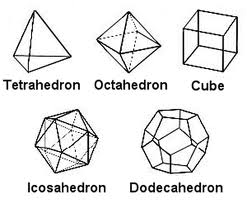
\includegraphics{platonic.jpg}
       \end{center}
       %\caption{The Platonic Solids}
       %\label{fig1}
%\end{figure}

Here are the names of the five platonic solids, which are pictured
above.  The {\em tetrahedron} is a $4$-sided solid with equilateral
triangles as faces; the {\em cube} is a $6$-sided solid with square
faces; the {\em octahedron} is an $8$-sided solid with equilateral
triangles as faces; the {\em dodecahedron} is a $12$-sided solid with
faces which are regular pentagons; and finally the {\em icosahedron}
is a $20$-sided solid with equilateral triangles for its faces.
 


\begin{example}[proper symmetry groups of the Platonic solids]
Let us begin by describing the {\em proper} symmetries (the rotations)
of the five Platonic solids. It is already a difficult problem to
count them in some effective way.

The proper symmetry group of the tetrahedron is the {\em tetrahedral
  group}\index{tetrahedral group}, denoted by $\mathbf{T}$.  It turns
out that $\mathbf{T} \cong \Alt_4$. This can be demonstrated by
considering a permutation representation of the tetrahedron. One can
number the vertices and write out the permutations corresponding to
the rotations, it turns out that these are precisely the elements of
$\Alt_4$. The details are tedious.  The isomorphism $\mathbf{T} \cong
\Alt_4$ means in particular that $|\mathbf{T}| = |\Alt_4| = 12$. So
there are 12 proper rotations of a tetrahedron.

The proper symmetries of the cube give us another group, called the
{\em octahedral group}\index{octahedral group}, and written as
$\mathbf{O}$. We have $|\mathbf{O}| = 24$.

The proper symmetries of the octahedron give us a group isomorphic
with $\mathbf{O}$, so we don't get a new group from this solid. 

This is due to the fact that the cube and the octahedron are {\em
  dual} to one another. To obtain the dual of a regular polyhedron,
put a dot in the center of each face, and let the dots be the vertices
of a new polyhedron.  This new polyhedron is the dual of the original
one. It is not hard to see that the symmetry group of a polyhedron
must be the same as the symmetry group of its dual.

The proper symmetries of the dodecahedron give us a third symmetry
group, called the {\em icosahedral group}\index{icosahedral group},
and denoted by the symbol $\mathbf{I}$. This group has $60$ elements;
in fact it is isomorphic with the alternating group $\Alt_5$.  The
proper symmetries of the icosahedron give us a group isomorphic with
$\mathbf{I}$, so we don't get a new group from this solid. This is due
to the fact that the icosahedron is the dual of the dodecahedron.


Summary: The proper symmetries of the five Platonic solids give us
just three new symmetry groups: $\mathbf{T}\cong \Alt_4$;
$\mathbf{O}$; and $\mathbf{I}\cong \Alt_5$. Two of them are isomorphic
to groups we have seen before, but the octahedral group $\mathbf{O}$
is new.
\end{example}


\begin{example}[improper symmetries of the Platonic solids]
\index{improper symmetry}%
As in the case of regular polygons, it turns out that there are
improper symmetries of all of the regular polyhedra. They are a bit
harder to describe, but it turns out that there are always as many
improper symmetries as there are proper ones, just as in the polygon
case.

When we include the improper symmetries, we get the full symmetry
group. The full symmetry group of each Platonic solid therefor has
twice as many elements as its proper symmetry group. We need to
develop more theory in order to say more about this topic, so we leave
this for now.
\end{example}





\section*{Exercises}
\begin{problems}

\item Explain why two finite groups of different cardinality cannot
  be isomorphic.

\item Prove that the proper symmetry group of the tetrahedron is
  isomorphic to the alternating group $\Alt_4$. One way to do this is
  via a permutation representation. (Number the vertices of the
  tetrahedron and regard symmetries as permutations of the vertices.)

\item Using the same idea as in the previous problem, prove that the
  full symmetry group of the tetrahedron is the symmetric group
  $\Sym_4$.

\item Explain why the symmetry group of a regular solid must be the
  same as that of its dual.

\item Describe the 24 proper symmetries of the cube in words. 

\end{problems}
\end{document}








%%%%%%%%%%%%%%%%%%%%%%%%%%%%%%% exercises %%%%%%%%%%%%%%%%%%
\item Prove that $r h r = h$ in $\D_n$ by giving a algebraic argument
  with matrices. Use a rotation matrix to represent $r$ and use an
  appropriate matrix to represent $h$ viewed as a reflection across
  the horizontal coordinate axis. (We can always position the regular
  $n$-gon so that this reflection is a symmetry, so we lose no
  generality by this assumption.)

\item We know that the rotation subgroup $\Rot_n$ of $\D_n$ is cyclic for
  any $n \ge 3$, generated by the basic rotation of $2\pi/n$
  radians. Let $\Rot_\infty$ be the rotation subgroup of $\D_\infty$. Is
  $\Rot_\infty$ cyclic, too? Justify your answer.

\item A {\em permutation matrix} is a matrix obtained from the
  identity matrix by some permutation of its columns. It is a matrix
  which has just one 1 in each row and column, and all other entries
  are zero.
\begin{enumerate}
\item Prove that $\Sym_n$ is isomorphic with the subgroup of
  permutation matrices in $\GL_n(F)$ by considering the matrix
  representation $f\colon \Sym_n \to \GL_n(F)$ given by $f(\alpha) =
  P_\alpha$, where for $\alpha \in \Sym_n$ we let $P_\alpha$ be the
  permutation matrix obtained by applying the permutation $\alpha$ to
  the columns of the identity matrix $I$.
\item Show that any permutation representation $\delta: G \to \Sym_n$
gives rise to a corresponding matrix representation $\rho: G \to
\GL_n(F)$ for any field $F$. (Thus permutation representations are
subsumed in the theory of matrix representations.)
\end{enumerate}

\item\label{exer:present-S_n} (Difficult) Find a presentation of
  $\Sym_n$ by generators and relations. We already know a nice
  generating set: namely the set of special transpositions
  $t_1=(1,2)$, $t_2=(2,3)$, $t_3=(3,4)$, $\dots,$ $t_n=(n-1, n)$.
  These special transpositions swap consecutive elements of the set
  $\mathbf{n} = \{1, \dots, n\}$. Find a set of relations between
  these generators $t_1, \dots, t_n$ that determines the symmetric
  group $\Sym_n$.

\item (Difficult) It has been previously observed that $\Sym_n$ is
  generated by any transposition along with any $n$-cycle. Put $t =
  (1,2)$ and $c = (1,2,3,\dots, n)$ in the cycle notation; then
  $\Sym_n$ is generated by the set $\{t, c\}$. Find a set of relations
  satisfied by these generators that determines $\Sym_n$.

%%%%%%%%%%%%%%%%%%%%%%%%%%%%%%%%%%%%%%%%%%%%%%%%%%%%%%%%%%%%%

\newpage
\documentclass[11pt]{article}
\usepackage[nohead,margin=1.50in]{geometry} %set margins
\usepackage{amsmath,amssymb,amsthm,pdiag,amscd,epic} %packages
\usepackage{graphicx}  
\usepackage{enumitem}
\setlist{topsep=1pt,itemsep=0pt,parsep=1pt,leftmargin=0.7cm}
\setenumerate[1]{label=(\alph*)}

\newenvironment{problems}
{
 \begin{enumerate}[topsep=1pt,itemsep=0pt,parsep=2pt,leftmargin=0.6cm,%
 label={\arabic*.}, ref=\arabic*] \small
}
{
 \end{enumerate}
}

%%% Define some theorem and example environments. The starred versions
%%% are un-numbered and the unstarred versions are numbered.
\newtheoremstyle{plain}
  {\topsep}   % ABOVESPACE
  {\topsep}   % BELOWSPACE
  {\slshape}  % BODYFONT
  {0pt}       % INDENT (empty value is the same as 0pt)
  {\bfseries} % HEADFONT
  {.}         % HEADPUNCT
  {5pt plus 1pt minus 1pt} % HEADSPACE
  {}          % CUSTOM-HEAD-SPEC

\swapnumbers
\newtheorem{thm}{Theorem}[section]
\newtheorem{lem}[thm]{Lemma}
\newtheorem{prop}[thm]{Proposition}
\newtheorem{cor}[thm]{Corollary}
\newtheorem*{thm*}{Theorem}
\newtheorem*{lem*}{Lemma}
\newtheorem*{prop*}{Proposition}
\newtheorem*{cor*}{Corollary}

\theoremstyle{definition}
\newtheorem{defn}[thm]{Definition}
\newtheorem{example}[thm]{Example}
\newtheorem{examples}[thm]{Examples}
\newtheorem{rmk}[thm]{Remark}
\newtheorem{conv}[thm]{Convention}
\newtheorem*{defn*}{Definition}
\newtheorem*{example*}{Example}
\newtheorem*{examples*}{Examples}
\newtheorem*{rmk*}{Remark}
\newtheorem*{conv*}{Convention}

%%% Define some convenient abbreviations for common mathematical
%%% notations.
\newcommand{\R}{\mathbb{R}} % use \R for the real numbers
\newcommand{\C}{\mathbb{C}} % use \C for the complex numbers
\newcommand{\Z}{\mathbb{Z}} % use \Z for the integers
\newcommand{\Q}{\mathbb{Q}} % use \Q for the rationals
\newcommand{\N}{\mathbb{N}} % use \N for the natural numbers
\newcommand{\compose}{\circ} % functional composition
\renewcommand{\implies}{\Rightarrow}
\renewcommand{\iff}{\Leftrightarrow}
\newcommand{\F}{{\mathbb F}}
\newcommand{\gen}[1]{\langle #1 \rangle}
\newcommand{\End}{\operatorname{End}}
\newcommand{\GL}{\mathrm{GL}}
\newcommand{\SL}{\mathrm{SL}}
\renewcommand{\O}{\mathrm{O}}
\newcommand{\SO}{\mathrm{SO}}
\newcommand{\U}{\mathrm{U}}
\newcommand{\SU}{\mathrm{SU}}
\newcommand{\g}{\mathfrak{g}}
\newcommand{\transpose}{\mathsf{T}}
\newcommand{\B}{\mathcal{B}}
\newcommand{\Rep}{\operatorname{Rep}}
\newcommand{\Mat}{\operatorname{Mat}}
\newcommand{\inner}[2]{\langle #1, #2 \rangle}
\newcommand{\sgn}{\operatorname{sgn}}
\newcommand{\n}{\underline{\mathbf{n}}}
\newcommand{\Sym}{\mathbb{S}}
\newcommand{\Alt}{\mathbb{A}}
\newenvironment{perm}[2]{\left(\begin{smallmatrix}#1 \\ #2}{\end{smallmatrix}\right)}
\newcommand{\Map}{\operatorname{Map}}
\newcommand{\Rot}{\Theta}
\newcommand{\D}{\mathbb{D}}


\allowdisplaybreaks
\parskip=2pt

%\title{Document Title}
%\author{author's name}

\begin{document}%\maketitle

%\appendix
\setcounter{section}{0}
\renewcommand{\thesection}{\Alph{section}}
\section{Appendix: Symmetries of polynomials} 
\noindent
Symmetry also plays an important role in the study of polynomial
equations\index{polynomial}, where the symmetry groups turn out to be
permutation groups. This was Lagrange's motivation to study
permutations.  But the definition of the symmetry group
\index{symmetry~group} of a polynomial, which is now known as its
\emph{Galois group}\index{Galois~group}, is not as accessible as the
symmetry group of a geometric object such as a polygon.  In this
appendix, we indicate the definition only in an intuitive way.

Our approach is difficult to use, so it turns out to be useful to
replace it by something less intuitive, but ultimately easier to work
with. The modern approach uses the theory of {\em field
  extensions}. Field extensions are typically studied in a second
course in abstract algebra, but they will not be considered here.



Suppose we have an $n$th degree polynomial $p(x)$ with real number
coefficients, say
\[
  p(x) = x^n + c_1x^{n-1} + c_2x^{n-2} + \cdots + c_{n-1}x + c_n . \tag{$*$}
\] 
The coefficients are the real numbers $c_j$ for $j = 1, \dots, n$.
According to the fundamental theorem of algebra
\index{fundamental~theorem!of~algebra}, the polynomial $p(x)$
has exactly $n$ roots $z_1, z_2, \dots, z_n$ in the complex number
system $\C$, where we agree to list multiple roots according to their
multiplicity. 

\begin{examples}
1. The polynomial $(x-1)^3 = x^3 - 3x^2+3x-1$ has three identical
roots $1, 1, 1$. There is one root of multiplicity three (a triple root).

2. The polynomial $(x^2-2)^2 = x^4 - 4x^2 + 4$ has roots $\sqrt{2}$,
$\sqrt{2}$, $-\sqrt{2}$, $-\sqrt{2}$. There are two real roots, each
of multiplicity two (two double roots).

3. The polynomial $(x^2+1)^2 = x^4+2x^2+1$ has roots $i, i, -i, -i$.
There are two non-real complex roots, each of multiplicity two (two
double roots). Here $i$ stands for the \emph{imaginary unit} in the
complex number system $\C$. (By definition, $i^2= -1$.) 

4. The polynomial $x(x^3-3x+2) = x^4 - 3x^2 + 2x$ has roots
$0,1,1,-2$.  This has one root of multiplicity two (one double
root). You can verify the roots by expanding the product
$x(x-1)^2(x+2)$.
\end{examples}

For definiteness, we assume that the polynomial $p(x)$ in equation
($*$) above has \emph{rational} coefficients, and that $p(x)$ is
irreducible, meaning that it cannot be factored into polynomials (with
rational coefficients) of strictly smaller degree. If $p(x)$ had such
a factorization, then we could deal separately with the two smaller
polynomials in order to solve $p(x) = 0$, so it makes sense to
restrict our attention to irreducible polynomials. 

We also assume, for simplicity, that the roots of $p(x)$ are all
\emph{distinct}, i.e., all the roots have multiplicity one.

\begin{defn}
Under the above assumptions, we define the {\em Galois
  group}\index{Galois~group} of the polynomial $p(x)$ to be the
permutation group consisting of all permutations of the roots $\{z_1,
\dots, z_n\}$ which preserve any algebraic relations among them.
\end{defn}



For a general polynomial\footnote{A general polynomial is one whose
  coefficients are represented by variables. For instance, $ax^2 + bx
  + c$ is the general polynomial of degree 2 (the general quadratic),
  $ax^3+bx^2+cx+d$ is the general polynomial of degree $3$ (the
  general cubic), and so on.} of degree $n$ there will be only trivial
relations among the roots, and thus the Galois group of the polynomial
will be unconstrained; it will thus be the full symmetric group
$\Sym_n$ consisting of all permutations of the $n$ roots. For special
polynomials, however, there can be non-trivial relations among the
roots imposing constraints on the permutations in the group; in such
cases the Galois group of the polynomial is often smaller than
$\Sym_n$. In all cases, the Galois group of an $n$th degree polynomial
will be a permutation group contained in $\Sym_n$.

Let's look at some concrete examples.

\begin{example}\label{ex:1}
Consider the polynomial $p(x)=x^4+x^3+x^2+x+1$.  Clearly we have
$$
p(x) = (x^5-1)/(x-1)
$$ as you can see by clearing denominators and expanding the resulting
product. The roots of $p(x)$ are $z_1=e^{2\pi i/5}$, $z_2 = e^{4\pi
i/5}$, $z_3 = e^{6\pi i/5}$, $z_4= e^{8\pi i/5}$. These complex
numbers all lie on the unit circle in the complex plane $\C$. (Recall
that $e^{i \theta} = \cos \theta + i \sin \theta$ for any angle
$\theta$, where the imaginary unit $i$ satisfies $i^2 = -1$.)
The roots satisfy the relations
$$
 z_2 = z_1^2, \quad z_3 = z_1^3, \quad z_4 = z_1^4 
$$ and any other relations (e.g., $z_3^2 = z_1$) are consequences of
these, along with the fact that $z_i^5 = 1$ for any $i = 1, \dots,
4$. We are looking for permutations of the four roots that preserve
these relations. If $\alpha$ is such a permutation, then
$\alpha(z_2)$, $\alpha(z_3)$, and $\alpha(z_4)$ will be determined by
$\alpha(z_1)$. Now $\alpha(z_1)$ can be $z_1$, $z_2$, $z_3$, or $z_4$.
We consider these possibilities separately.

If $\alpha(z_1)=z_1$ then $\alpha(z_2) = \alpha(z_1)^2 = z_2$,
$\alpha(z_3) = \alpha(z_1)^3 = z_3$, and $\alpha(z_4) = \alpha(z_1)^4
= z_4$. Thus $\alpha = (1)$ is the identity
permutation. 

If $\alpha(z_1)=z_2$ then $\alpha(z_2) = \alpha(z_1)^2 = z_2^2 = z_4$,
$\alpha(z_3) = \alpha(z_1)^3 = z_2^3 = z_1$, and $\alpha(z_4) =
\alpha(z_1)^4 = z_2^4 = z_3$. Thus $\alpha$ is the 4-cycle
$(1,2,4,3)$.

If $\alpha(z_1)=z_3$ then $\alpha(z_2) = \alpha(z_1)^2 = z_3^2 = z_1$,
$\alpha(z_3) = \alpha(z_1)^3 = z_3^3 = z_4$, and $\alpha(z_4) =
\alpha(z_1)^4 = z_3^4 = z_2$. Thus $\alpha$ is the 4-cycle
$(1,3,4,2)$.

Finally, if $\alpha(z_1)=z_4$ then $\alpha(z_2) = \alpha(z_1)^2 =
z_4^2 = z_3$, $\alpha(z_3) = \alpha(z_1)^3 = z_4^3 = z_2$, and
$\alpha(z_4) = \alpha(z_1)^4 = z_4^4 = z_1$. Thus $\alpha =
(1,4)(2,3)$.

From these calculations it follows that the symmetry group of the
polynomial $x^4+x^3+x^2+x+1$ is the cyclic group generated by
the cycle $(1,2,4,3)$. This Galois group $G$ has order $4$. 
\end{example}


\begin{example} \label{ex:2}
Now consider the polynomial $p(x) = x^4 -10x^2 + 1$.
We can factor $p(x)$ as follows:
\begin{align*}
p(x) = (x^4 - 2x^2 + 1) - 8x^2 &= (x^2-1)^2 - (x\sqrt{8})^2\\
&= (x^2-1-2\sqrt{2}x)(x^2-1+2\sqrt{2}x) \\
&= (x^2-2\sqrt{2}x-1)(x^2+2\sqrt{2}x-1)
\end{align*}
and we can find its roots by setting each quadratic factor to zero and
using the quadratic formula. The roots are $z_1 = \sqrt{2}+\sqrt{3}$,
$z_2 = -\sqrt{2}+\sqrt{3}$, $z_3 = \sqrt{2}-\sqrt{3}$, $z_4 =
-\sqrt{2}-\sqrt{3}$. Notice that all the roots are real numbers in
this case.

The roots satisfy the relations:
\begin{align*}
z_1+z_4 &= 0 \\
z_2+z_3 &= 0 \\
(z_1+z_2)^2 &= 12 \\
(z_1+z_3)^2 &= 8 \\
(z_2+z_4)^2 &= 8 \\
(z_3+z_4)^2 &= 12 
\end{align*}
and again all other relations are consequences of these. We want all
permutations of the four roots which preserve these relations. You can
check that the permutations $(1,2)(3,4)$, $(1,3)(2,4)$, $(1,4)(2,3)$,
and the identity $(1)$ preserve the relations. No other permutation
does. Thus the symmetry group of the polynomial $p(x) = x^4 -10x^2 +
1$ is $$G = \{ (1), (1,2)(3,4), (1,3)(2,4), (1,4)(2,3) \}.$$ This is a
group of order four. It turns out that it is isomorphic with the Klein
four-group.\index{Klein~four~group}
\end{example}


\setcounter{equation}{0} 
\subsection*{The cubic formula}
We now consider the cubic formula, the degree three analogue of the quadratic
formula.  Given a general cubic polynomial equation:
\begin{equation}\label{eq:cubic}
  x^3 - bx^2 + cx - d = 0
\end{equation} 
with undetermined (i.e., general) coefficients, we denote its complex
roots by $z_1$, $z_2$, and $z_3$. To solve the equation, we first
substitute $x=y+b/3$ and obtain (after expanding) the {\em reduced
  cubic} equation\index{cubic equation}
\begin{equation}\label{eq:reduced-cubic}
  y^3 +py - q = 0
\end{equation}
where $p = c-b^2/3$ and $q = d - bc/3 + 2b^3/27$. The roots of the
reduced cubic are given by \emph{Cardano's formula}, first published
in the year 1545.

\begin{thm*}[Cardano 1545]\index{Cardano's formula}
The roots of the reduced cubic $y^3 +py - q = 0$ are given by
\begin{equation}\label{eq:Cardano}
\begin{aligned}
y_1 &= \sqrt[3]{\frac{q}{2}+\sqrt{R}} + \sqrt[3]{\frac{q}{2}-\sqrt{R}}\\
y_2 &= \omega^2 \sqrt[3]{\frac{q}{2}+\sqrt{R}} 
     + \omega \sqrt[3]{\frac{q}{2}-\sqrt{R}}\\
y_3 &= \omega \sqrt[3]{\frac{q}{2}+\sqrt{R}} 
     + \omega^2 \sqrt[3]{\frac{q}{2}-\sqrt{R}}\\
\end{aligned}
\end{equation}
where 
\[
  R = \frac{q^2}{4} + \frac{p^3}{27}; \qquad \omega = \frac{-1 + i
    \sqrt{3}}{2}.
\]
\end{thm*}

Note that $\omega = e^{i 2\pi/3}$ and therefore $\omega^3 =
1$. Moreover, $\omega^2 + \omega + 1 = 0$. The complex number $\omega$
is called a {\em primitive cube root of unity}.

To find the roots $z_i$ ($i = 1,2,3$) of the original cubic we only
have to add $b/3$ to the $y_i$.  This solves the original cubic equation,
and the solution is in terms of certain radicals (square and cube
roots), namely those that occur in the expressions for the $y_i$. 



\subsection*{Lagrange's method for solving a cubic}
\index{Lagrange's~method}%
In an important paper published in 1770, Lagrange noticed that the
radicals appearing in the solution to the
original cubic are expressible as functions of the roots $z_i$
themselves. This observation was the beginning of the link between
group theory and polynomial equations.

To see this for the cube roots, we multiply the equations for the
$y_i$ by 1, $\omega$, $\omega^2$ respectively and add, obtaining
$$
3 \sqrt[3]{\frac{q}{2}+\sqrt{R}} = y_1 + \omega y_2 + \omega^2 y_3.
$$
Thus if we substitute $y_i = z_i - b/3$ we obtain
$$
3 \sqrt[3]{\frac{q}{2}+\sqrt{R}} = z_1 + \omega z_2 + \omega^2 z_3.
$$
Denote this value by $\varphi_1$, and set
$\varphi_3=\omega^2\varphi_1$, $\varphi_5=\omega\varphi_1$, so that we
have equalities
\begin{align*}
\varphi_1 &= 3 \sqrt[3]{\frac{q}{2}+\sqrt{R}} \\
\varphi_3 &= 3 \omega^2 \sqrt[3]{\frac{q}{2}+\sqrt{R}} \\
\varphi_5 &= 3 \omega \sqrt[3]{\frac{q}{2}+\sqrt{R}}.
\end{align*}
Going back and multiplying the equations for $y_1$, $y_2$, $y_3$ by
$1$, $\omega^2$, $\omega$ respectively, we obtain after adding them
and substituting for $y_i = z_i - b/3$ the equality
$$
3 \sqrt[3]{\frac{q}{2}-\sqrt{R}} = z_1 + \omega^2 z_2 + \omega z_3.
$$ 
Let us denote this value by $\varphi_2$, and set $\varphi_4 =
\omega \varphi_2$, $\varphi_6 = \omega^2 \varphi_2$. Then we have
equalities 
\begin{align*}
\varphi_2 &= 3 \sqrt[3]{\frac{q}{2}-\sqrt{R}} \\
\varphi_4 &= 3 \omega \sqrt[3]{\frac{q}{2}-\sqrt{R}} \\
\varphi_6 &= 3 \omega^2 \sqrt[3]{\frac{q}{2}-\sqrt{R}}.
\end{align*}
We can also express $\sqrt{R}$ in terms of the roots $z_i$ by cubing
the equations for $\varphi_1$ and $\varphi_2$ and subtracting. Doing
this, we obtain
$$ 54 \sqrt{R} = (z_1+\omega z_2+\omega^2 z_3)^3 - (z_1+\omega^2
z_2+\omega z_3)^3
$$
and after expanding, simplifying, and factoring we have
$$
18\sqrt{R} = 3i (z_1-z_2)(z_1-z_3)(z_2-z_3).
$$
Thus all the radicals appearing in the formulas for the roots are
expressible as nice functions of the roots themselves. 


Lagrange noticed that the roots of the general cubic are obtainable
from the six values $\varphi_i$ ($i = 1, \dots, 6$), because we have
the system of linear equations 
\begin{equation}\label{eq:Lagrange-system}
\begin{aligned}
\varphi_1 &= z_1 + \omega z_2 + \omega^2 z_3\\
\varphi_2 &= z_1 + \omega^2 z_2 + \omega z_3\\
b & = z_1 + z_2 +z_3
\end{aligned}
\end{equation}
which can easily be solved for the roots $z_1$, $z_2$, $z_3$ by first
adding them as they stand, then adding them after multiplying by
$\omega^2$, $\omega$, 1, and then adding them again after multiplying
by $\omega$, $\omega^2$, 1, respectively.

Lagrange also pointed out that we can compute the six values
$\varphi_i$ as follows. Set $A_1 = q/2 + \sqrt{R}$ and $A_2 = q/2 -
\sqrt{R}$. Then we have the equations
$$
\left(\frac{\varphi_i}{3}\right)^3 = A_1 \qquad (i = 1,3,5)
$$
and 
$$
\left(\frac{\varphi_i}{3}\right)^3 = A_2 \qquad (i = 2,4,6).
$$ 
In other words, the six $\varphi_i$ are obtained by solving the
equations $X^3 = 27A_1$ and $X^3 = 27A_2$. (Note that if $\varphi$ is one
root, say the cube root of $A_i$, then the other two roots must be $\omega
\varphi$ and $\omega^2 \varphi$.)

Examining the expressions defining $A_1$ and $A_2$, we see that we can
find the $A_i$ by solving the quadratic equation
\begin{equation}\label{eq:Lagrange-resolvant}
   A^2 - q A - p^3/27 = 0
\end{equation}
for $A$. In this way Lagrange reduced the solution of the cubic to the
solution of a quadratic. (He called this associated quadratic equation
the {\em resolvent}.) By first solving the resolvent quadratic and
then solving the system \eqref{eq:Lagrange-system} you can solve the
cubic using Lagrange's method.


Lagrange also similarly analyzed the general
quartic\index{quartic~equation} (degree 4) polynomial equation,
reducing it to a cubic resolvent equation. He must have been quite
excited at that point, thinking that he had discovered a general
scheme to solve all polynomial equations inductively by reducing them
to a resolvent equation of degree one less than the given equation.
However, when he looked at the very next case, the general quintic
(degree 5) equation, he found that the resolvent equation had degree
6. This was a strong indication that the general quintic might be
unsolvable in terms of radicals, and indeed N.\ H.\ Abel proved that
very result in 1826.

\begin{thm*}[Abel 1826]\index{Abel's theorem}
  The general quintic (degree five) polynomial equation cannot be
  solved in terms of radicals.
\end{thm*}

Galois further developed group theory and the theory of polynomial
equations. He was able to give necessary and sufficient conditions on
the symmetry group of an arbitrary polynomial (of any degree) for it
to be solvable in terms of radicals. His theorem is a vast
generalization of Abel's theorem, in that it applies to polynomials of
any degree. Galois discovered the theorem in 1830 at the age of 18; he
was shot and killed in a duel at the age of 20. The theorem remained
unpublished until 1846, and it wasn't until the late 1800s that
mathematicians generally understood the significance of his results.





\section*{Exercises}

\begin{problems}

\item Solve the polynomial equation $p(x)=0$ of \ref{ex:2} by setting
  $y=x^2$ and solving the resulting quadratic equation, and then
  finding $x$ by taking square roots of $y$.  Compare your answer with
  the roots of $p(x)$ given in \ref{ex:2}. Can you explain?

\item One strategy for solving a polynomial equation $p(x)=0$ is to
  guess a root $z_1$ of the equation. The guess can be checked by
  substitution in $p(x)$. If $p(z_1)=0$ then $z_1$ is a root. Once you
  have found a root $z_1$, you can use long division of polynomials to
  divide $p(x)$ by $x-z_1$. Since roots correspond to linear factors,
  the fact that $z_1$ is a root means that when you divide you will
  obtain a quotient polynomial $q(x)$ such that $p(x) = (x-z_1) q(x)$.
  Now you have reduced the original problem, of solving $p(x)=0$, to
  the smaller problem of solving $q(x)=0$. By repeating the method,
  you can eventually factor $p(x)$ completely into linear factors,
  thus solving the polynomial equation.  The problem with this
  strategy is that it is not always possible to guess a
  solution. Thus, the method may never get started, or it may stall
  somewhere along the way. However, it works in a surprising number of
  cases. Use this method to solve the following cubic equations, using
  the given guess:
  \begin{enumerate}
  \item $x^3+1 = 0$; guess $z_1 = -1$.
  \item $x^3-3x^2+3x-1 = 0$; guess $z_1 = 1$.
  \item $x^3+2x+3 = 0$; find your own guess.
  \end{enumerate}

\item If a polynomial $p(x)$ with \emph{integer} coefficients has a
  rational root (a root of the form $\frac{r}{s}$ where $r,s$ are
  integers), then we can always find it using the \emph{rational roots
  theorem}.
  \begin{thm*}
    Suppose that
    $p(x) = a_0 x^n + a_1 x^{n-1} + \cdots + a_{n-1} x + a_n$, where
    $a_0 \ne 0$ and $a_k \in \Z$ for all $k = 0, 1, \dots, n$. If
    $z_1 = \pm \frac{r}{s}$ is a rational root of $p(x)$ then
    $s \mid a_0$ ($s$ divides $a_0$) and $r \mid a_n$ ($r$ divides
    $a_n$).
  \end{thm*}
  Use the rational roots theorem to find all rational roots (if any)
  of the following polynomials:
  \begin{enumerate}
  \item $3x^3+4x-7$.
  \item $x^3+x^2+x+2$.
  \item $x^3+8$.
  \end{enumerate}

\item Find all the roots of the polynomials in parts (a), (c) of the
  previous problem.

\item Show that the symmetry group $G$ of Example \ref{ex:2} is
  isomorphic with the Klein 4-group. (The Klein 4-group was introduced
  in Section 7.)

\item Use Cardano's formula or Lagrange resolvents to solve the
  following cubic equations:
  \begin{enumerate}
  \item $x^3 - 3x + 2 = 0$. 
  \item $x^3 - 9x^2 + 24x - 16 = 0$.
  \item $x^3 + 3x^2 + 6x + 2 = 0$.
  \item $x^3 + 3 x - 4 = 0$. 
  \end{enumerate}
Show the steps of your calculations. Notice that by inspection $1$ is
a root of the first and last equations; did your calculations in part
(d) reveal that fact? Do you think something is wrong?


\item Let $\omega = e^{2\pi i/n} = \cos(2\pi/n) + i \sin(2\pi/n)$ be a
  primitive $n$th root of unity. Prove that the roots of $x^n - 1 = 0$
  are the complex numbers $z_k = \omega^k$ for $k = 0, 1, \dots,
  n-1$. (This is a complete list of $n$ distinct roots.) 
  \begin{enumerate}
  \item Compute $\omega^n$.
  \item Why is the set $G$ of roots of the polynomial a group? What type
    of group is it?
  \item If you plot the roots in the complex plane, they form the set
    of vertices of what geometric figure?
  \end{enumerate}

\end{problems}
\renewcommand{\thesection}{\arabic{section}}
\end{document}







\subsection*{Galois group of the general cubic} 
Let us determine the Galois group of the general cubic. We continue to
use all the notation introduced in \ref{ss:cubic}. Tabulating all the
expressions for the $\varphi_i$ we have
\begin{align*}
\varphi_1 &= z_1+\omega z_2 + \omega^2 z_3 \\
\varphi_3 &= z_2+\omega z_3 + \omega^2 z_1 \\
\varphi_5 &= z_3+\omega z_1 + \omega^2 z_2 \\
\varphi_2 &= z_1+\omega z_3 + \omega^2 z_2 \\
\varphi_4 &= z_2+\omega z_1 + \omega^2 z_3 \\
\varphi_6 &= z_3+\omega z_2 + \omega^2 z_1.
\end{align*}
If we examine these expressions, we might notice that all the six
values $\varphi_i$ are obtained from $\varphi_1$ by permuting in all
possible ways the symbols $z_1, z_2, z_3$. This observation led
Lagrange to investigate permutation groups.

The six equations above are (some of) the relations which the roots of
the general cubic equation must satisfy, and any permutation of the
roots will preserve them. This suggests that the Galois group of the
general cubic should be the entire symmetric group $\Sym_3$, and
indeed that is so (but not so easy to prove). Some other relations
satisfied by the roots are
\begin{align*}
b &= z_1+z_2+z_3\\
c &= z_1z_2+z_1z_3+z_2z_3\\
d &= z_1 z_2 z_3.
\end{align*}
Clearly these relations are also preserved by all permutations of the
roots.

%%%%%%%%%%%%%%%%%%%%%%%%%%%%%%% exercises %%%%%%%%%%%%%%%%%%
\item Prove that $r h r = h$ in $\D_n$ by giving a algebraic argument
  with matrices. Use a rotation matrix to represent $r$ and use an
  appropriate matrix to represent $h$ viewed as a reflection across
  the horizontal coordinate axis. (We can always position the regular
  $n$-gon so that this reflection is a symmetry, so we lose no
  generality by this assumption.)

\item We know that the rotation subgroup $\Rot_n$ of $\D_n$ is cyclic for
  any $n \ge 3$, generated by the basic rotation of $2\pi/n$
  radians. Let $\Rot_\infty$ be the rotation subgroup of $\D_\infty$. Is
  $\Rot_\infty$ cyclic, too? Justify your answer.

\item A {\em permutation matrix} is a matrix obtained from the
  identity matrix by some permutation of its columns. It is a matrix
  which has just one 1 in each row and column, and all other entries
  are zero.
\begin{enumerate}
\item Prove that $\Sym_n$ is isomorphic with the subgroup of
  permutation matrices in $\GL_n(F)$ by considering the matrix
  representation $f\colon \Sym_n \to \GL_n(F)$ given by $f(\alpha) =
  P_\alpha$, where for $\alpha \in \Sym_n$ we let $P_\alpha$ be the
  permutation matrix obtained by applying the permutation $\alpha$ to
  the columns of the identity matrix $I$.
\item Show that any permutation representation $\delta: G \to \Sym_n$
gives rise to a corresponding matrix representation $\rho: G \to
\GL_n(F)$ for any field $F$. (Thus permutation representations are
subsumed in the theory of matrix representations.)
\end{enumerate}

\item\label{exer:present-S_n} (Difficult) Find a presentation of
  $\Sym_n$ by generators and relations. We already know a nice
  generating set: namely the set of special transpositions
  $t_1=(1,2)$, $t_2=(2,3)$, $t_3=(3,4)$, $\dots,$ $t_n=(n-1, n)$.
  These special transpositions swap consecutive elements of the set
  $\mathbf{n} = \{1, \dots, n\}$. Find a set of relations between
  these generators $t_1, \dots, t_n$ that determines the symmetric
  group $\Sym_n$.

\item (Difficult) It has been previously observed that $\Sym_n$ is
  generated by any transposition along with any $n$-cycle. Put $t =
  (1,2)$ and $c = (1,2,3,\dots, n)$ in the cycle notation; then
  $\Sym_n$ is generated by the set $\{t, c\}$. Find a set of relations
  satisfied by these generators that determines $\Sym_n$.

%%%%%%%%%%%%%%%%%%%%%%%%%%%%%%%%%%%%%%%%%%%%%%%%%%%%%%%%%%%%%


\chapter{Modular Arithmetic}
\documentclass[11pt]{article}
\usepackage[nohead,margin=1.50in]{geometry} %set margins
\usepackage{amsmath,amssymb,amsthm,pdiag} %AMS packages for math stuff
\usepackage{multicol} % for use in HW section
\usepackage{enumitem}
  \setlist{topsep=1pt,itemsep=0pt,parsep=1pt}
  \setenumerate[1]{label=(\alph*)}

\newenvironment{problems}
{
 \begin{enumerate}[topsep=1pt,itemsep=0pt,parsep=2pt,leftmargin=0.6cm,%
 label={\arabic*.}, ref=\arabic*] \small
}
{
 \end{enumerate}
}

%%% Define some theorem and example environments. The starred versions
%%% are un-numbered and the unstarred versions are numbered.
\newtheoremstyle{plain}
  {\topsep}   % ABOVESPACE
  {\topsep}   % BELOWSPACE
  {\slshape}  % BODYFONT
  {0pt}       % INDENT (empty value is the same as 0pt)
  {\bfseries} % HEADFONT
  {.}         % HEADPUNCT
  {5pt plus 1pt minus 1pt} % HEADSPACE
  {}          % CUSTOM-HEAD-SPEC

\swapnumbers
\newtheorem{thm}{Theorem}[section]
\newtheorem{lem}[thm]{Lemma}
\newtheorem{prop}[thm]{Proposition}
\newtheorem{cor}[thm]{Corollary}
\newtheorem*{thm*}{Theorem}
\newtheorem*{lem*}{Lemma}
\newtheorem*{prop*}{Proposition}
\newtheorem*{cor*}{Corollary}

\theoremstyle{definition}
\newtheorem{defn}[thm]{Definition}
\newtheorem{example}[thm]{Example}
\newtheorem{examples}[thm]{Examples}
\newtheorem{rmk}[thm]{Remark}
\newtheorem{rmks}[thm]{Remarks}
\newtheorem{conv}[thm]{Convention}
\newtheorem*{defn*}{Definition}
\newtheorem*{example*}{Example}
\newtheorem*{examples*}{Examples}
\newtheorem*{rmk*}{Remark}
\newtheorem{rmks*}{Remarks}
\newtheorem*{conv*}{Convention}

%%% Define some convenient abbreviations for common mathematical
%%% notations.
\newcommand{\R}{\mathbb{R}} % use \R for the real numbers
\newcommand{\C}{\mathbb{C}} % use \C for the complex numbers
\newcommand{\Z}{\mathbb{Z}} % use \Z for the integers
\newcommand{\Q}{\mathbb{Q}} % use \Q for the rationals
\newcommand{\N}{\mathbb{N}} % use \N for the natural numbers
\newcommand{\F}{{\mathbb F}}
\newcommand{\compose}{\circ} % functional composition
\renewcommand{\implies}{\Rightarrow}
\renewcommand{\iff}{\Leftrightarrow}
\newcommand{\gen}[1]{\langle #1 \rangle}
\newcommand{\End}{\operatorname{End}}
\newcommand{\GL}{\mathrm{GL}}
\newcommand{\SL}{\mathrm{SL}}
\renewcommand{\O}{\mathrm{O}}
\newcommand{\SO}{\mathrm{SO}}
\newcommand{\U}{\mathrm{U}}
\newcommand{\SU}{\mathrm{SU}}
\newcommand{\g}{\mathfrak{g}}
\newcommand{\transpose}{\mathsf{T}}
\newcommand{\B}{\mathcal{B}}
\newcommand{\Rep}{\operatorname{Rep}}
\newcommand{\Mat}{\operatorname{Mat}}
\newcommand{\inner}[2]{\langle #1, #2 \rangle}
\newcommand{\sgn}{\operatorname{sgn}}
\newcommand{\n}{\underline{\mathbf{n}}}
\newcommand{\Sym}{\mathbb{S}}
\newcommand{\Alt}{\mathbb{A}}
\newenvironment{perm}[2]{\left(\begin{smallmatrix}#1 \\ #2}{\end{smallmatrix}\right)}
\newcommand{\lcm}{\operatorname{lcm}}
\newcommand{\res}{\operatorname{res}}


\allowdisplaybreaks
\parskip=2pt

%\title{Document Title}
%\author{author's name}

\begin{document}%\maketitle
\setcounter{section}{10}


\section{Modular arithmetic}\noindent
Modular arithmetic is a novel finite system of arithmetic used in
public-key cryptography\index{cryptography} in order to provide
security for internet transactions. It is also used in algebraic
coding theory, the mathematical theory underlying the encoding of
information on DVDs, satellite communications, etc. And it provides
new examples of groups. We begin with some elementary number theory.

\begin{lem}[division algorithm]\index{division~algorithm}
Let $n$ be a positive integer.  Let $m$ be any integer.
There exist unique integers $q$, $r$ such that
\[
m = qn + r \quad\text{and}\quad 0 \le r < n. 
\]
The integers $q$, $r$ are called the {\em quotient} and {\em
  remainder}, respectively.
\end{lem}

\begin{proof}\index{well-ordering principle}
Recall the \emph{well-ordering principle} of natural numbers, which
states that any nonempty subset of $\N = \{0,1,2,\dots\}$ must have a
least element. Let
\[
  S = \{ m - kn \mid k \in \Z \text{ and } m - kq \ge 0 \}.
\]
By construction, $S$ is a subset of $\N$. We need to show it is
nonempty. If $m \ge 0$ then $m = m-0\cdot n \in S$. If $m < 0$ then
$m-mn = m(1-n) \ge 0$ because $1-n \le 0$, hence $m-mn$ is in $S$. In
either case $S$ is not empty. By the well ordering principle, the set
$S$ has a least element. Let $r$ be the least element of $S$ and let
$q$ be the corresponding value of $k$. Then $m - qn = r$, so $m =
qn+r$. Moreover, $r \ge 0$ since $r \in S$. Finally, $r < n$ since
otherwise $r-n$ would be in $S$, contradicting the fact that $r$ is
the least element of $S$.
\end{proof}

When $m$ is positive, the usual procedure by which we find the
quotient $q$ and remainder $r$ is called long division, as you
undoubtedly recall. 

Given a real number $x$, there is a unique integer $k$ such that $k
\le x < k+1$. The integer $k$ is called the \emph{floor}\index{floor}
of $x$, written as $\lfloor x \rfloor = k$. The floor function is also
known as the \emph{greatest integer} function.  Then for a given pair
of integers $m,n$ we have:
\[
  q = \lfloor m/n \rfloor, \quad r = m-qn.
\]
Note that when $m<0$ we need to pay attention. For instance, we have
$20 = 2 \cdot 7 + 6$ for $20 \div 7$, but $-20 = -3 \cdot 7 + 1$ for
$-20 \div 7$. 





\begin{defn}
  Let $n$ be a positive integer greater than 1. We call $n$ the
  \emph{modulus}\index{modulus}. The set \index{Z@$\Z_n$}$\Z_n = \{0,
  1, \dots, n-1 \}$ is called the set of \emph{residues} modulo $n$.
  This is the set of remainders for long division by $n$, so
  \emph{residue}\index{residue} is another word for \emph{remainder}.
\end{defn}


\begin{defn} [residue function]
  Let a modulus $1<n \in \Z$ be given. Given an integer $m$, let $q,r$
  be the unique integers such that $m = qn + r$ and $0 \le r < n$.
  Then set $\res_n(m) = r$. The resulting function
  $\res_n: \Z \to \Z_n$ is a surjection from the set $\Z$ of integers
  onto the set $\Z_n$ of residues modulo $n$.
\end{defn}

We should read $\res_n(m)$ as ``the residue of $m$ modulo $n$.'' It is
just the remainder of dividing $m$ by $n$, so we can always compute it
by long division.

Now we define addition and multiplication on the set $\Z_n$. 

\begin{defn}
  Let $n>1$ be a fixed integer modulus. Given residues $a,b \in \Z_n$,
  we define
  \[
  a \oplus b = \res_n(a+b), \qquad a \odot b = \res_n(ab).
  \]
  We call the binary operations $\oplus, \odot$ \emph{residue
    addition} and \emph{residue multiplication}.
\end{defn}

The residue addition and multiplication rules just defined can be
remembered as a two-step procedure: first, add or multiply in $\Z$ as
usual, then take the residue of the result modulo $n$.

\begin{rmk}
  We use new symbols $\oplus, \odot$ for residue addition and
  multiplication, in order to distinguish these new and novel
  operations from the usual ones. Eventually, we will drop the extra
  circle around the symbol and use the usual addition and
  multiplication symbols. For now, it is useful to use different
  notation in order to avoid confusion.
\end{rmk}


\begin{example} 
The addition and multiplication tables for $\Z_2$ are given below. 
\[
\begin{array}{|c|cc|} \hline
\oplus&0&1\\ \hline 0&0&1\\ 1&1&0\\ \hline
\end{array}
\qquad \qquad
\begin{array}{|c|cc|} \hline
\odot &0&1\\ \hline
0&0&0\\
1&0&1\\
\hline
\end{array}
\]
We will see later that the above addition table defines a group. This
group appears in computer science as the table defining the behavior
of a binary half-adder circuit, which is a basic circuit used in all
digital computers. 
\end{example}



\begin{example} 
The addition and multiplication tables for $\Z_4$ are compiled below. 
\[
\begin{array}{|c|cccc|} \hline
\oplus&0&1&2&3\\ \hline 
0&0&1&2&3\\ 1&1&2&3&0\\ 
2&2&3&0&1\\ 3&3&0&1&2\\ \hline
\end{array}
\qquad \qquad
\begin{array}{|c|cccc|} \hline
\odot &0&1&2&3\\ \hline
0&0&0&0&0\\
1&0&1&2&3\\ 
2&0&2&0&2\\ 
3&0&3&2&1\\ \hline
\end{array}
\]
This is more interesting. Notice that the tables are ``closed''
systems, in which the combination of two elements produces another one
in the set $\Z_4$. Also notice the novel equation $2 \odot 2 = 0$. In
residue arithmetic, two nonzero elements can multiply to produce $0$,
which is somewhat strange at first sight.
\end{example}

Residue arithmetic is also called \emph{modular arithmetic}. Looking
at the addition tables (for the operation $\oplus$) in the above
examples, we suspect that they might be groups, because the tables
``look'' similar to multiplication tables for other groups we have
seen, and that is indeed the case, as we will see later. But not so
for the multiplication tables (for the operation $\odot$). They are
\emph{never} examples of groups, because there is no inverse of $0$
in the tables. Nevertheless, there is always at least one group inside
the multiplication table, if you know how to look for it. We will
return to this question later, once we have developed a better
definition of group. For now, the focus is on understanding modular
arithmetic.


It is notable that we can make sense of subtraction in $\Z_n$. Here
are the appropriate definitions, which follow the same pattern as the
definitions of negatives and subtraction in the integers.

\begin{defn}
  The \emph{negative} $\ominus a$ of a residue $a \in \Z_n$ is defined to be
  \[
  \ominus a = 
  \begin{cases}
    0 & \text{ if } a = 0 \\
    n-a & \text{ if } a \ne 0.
  \end{cases}
  \]
\end{defn}

Once we have negatives, we can define subtraction in terms of adding
the negative, which is how subtraction is defined for integers and
real numbers.

\begin{defn}
  For any $a,b \in \Z_n$, we define $a \ominus b = a \oplus (\ominus b)$. 
\end{defn}

Notice that $a \oplus ( \ominus a) = 0$ and $(\ominus a) \oplus a =
0$, for any $a \in \Z_n$.


\begin{thm}\label{thm:ressub}
   For any $a,b \in \Z_n$, we have $a \ominus b = \res_n(a-b)$. 
\end{thm}

The proof is a straightforward exercise.

The theorem gives us another way to compute $a \ominus b$. Depending
on the situation, one way might be more convenient than the other, so
it can be useful to have both.

\begin{rmk}[notational convention]
  It soon becomes tedious to always write $\oplus, \odot, \ominus$ for
  the residue operations. The convention is to replace these symbols
  by their corresponding uncircled symbols $+, \cdot, -$ from ordinary
  arithmetic. This convention results in equations such as:
  \[
    5+5 = 0,\quad 6+7 = 3,\quad 6 \cdot 7 = 2,\quad 4 \cdot 5 = 0,
    \quad -6 = 4,\quad 5-6 = 9
  \]
  all of which are valid equations in $\Z_{10}$. This is confusing
  only if you forget that $+$ really means $\oplus$, $\cdot$ means $\odot$,
  and $-$ means $\ominus$.  

  Furthermore, it is conventional to omit the multiplication symbol
  $\cdot$ in cases where doing so will not cause confusion. So, if
  $a,b$ are variables representing values in some residue system
  $\Z_n$, we usually interpret $ab$ as $a \cdot b$, just as we do in
  ordinary algebra.
\end{rmk}

Modular arithmetic\index{modular~arithmetic} is actually similar to
arithmetic everyone already carries out with clocks. In a standard
clock, there are 12 numbers arranged in a circle, and we all
understand that 3 hours after 11 o'clock is 2 o'clock. This is the
same as the equation $11+3 = 2$ in $\Z_{12}$. The only difference
between addition in $\Z_{12}$ and clock addition is that in $\Z_{12}$
we have renamed the modulus $12$ to $0$.

We can visualize modular arithmetic modulo $n$ similarly, by thinking
of a clock with the residues $0, 1, \dots, n-1$ equally spaced around
its face. Whenever we reach $n$ hours, the clock resets to $0$. 




\section*{Exercises}
\begin{problems}

\item The \emph{floor} of a real number $x$ (written $\lfloor x
  \rfloor$) is the greatest integer $k$ such that $k \le x$.  Given
  integers $m,n$ with $n > 0$, show that $q = \lfloor m/n \rfloor$ is
  the integer quotient such that $m = qn+r$ with $0 \le r < n$.


\item A pocket calculator (or computer) that produces decimal
  approximations for quotients can often be used to carry out the
  division algorithm in the set of integers. Given integers $m,n$ with
  $n > 0$, to find the integer quotient $q$ such that $m = qn+r$ with
  $0 \le r < n$, simply calculate $m \div n$ on the device and then
  take $q$ to be the integer part (the floor) of the result. Once you
  have found $q$, of course $r = m - qn$. Use this to find the integer
  quotient $q$ and remainder $r$ for each of the following division
  problems:
  \begin{multicols}{2}
  \begin{enumerate}[topsep=0pt,parsep=0pt]
  \item $1000 \div 31$.
  \item $-1000 \div 31$.
  \item $16075 \div 652$.
  \item $-16075 \div 652$.
  \end{enumerate}
  \end{multicols}
  This approach is slightly dangerous, because if the numbers $m,n$
  are big enough, machine calculation can be subject to roundoff
  error. If you are using a pocket calculator, try to find a case
  where it produces an incorrect integer quotient.

\item Compute the following in the modular system $\Z_{12}$.
  \begin{enumerate}
  \item $7+5$, $5+5$, $11+11$, $-1 + (-1)$.
  \item $3 \cdot 3$, $7 \cdot 5$, $5 \cdot 5$, $11 \cdot 11$, $(-1)
    \cdot (-1)$.
  \item $3-3$, $5-7$, $-2-10$, $5-(-3)$, $5-(-11)$,
    $-2-(-10)$.
  \end{enumerate}

\item Make addition and multiplication tables for $\Z_3$.

\item Make addition and multiplication tables for $\Z_5$.

\item Make addition and multiplication tables for $\Z_6$.

\item Make addition and multiplication tables for $\Z_7$.

\item Make addition and multiplication tables for $\Z_8$.

\item Compute the following in the modular system $\Z_{1201}$.
  \begin{enumerate}
  \item $75+500$, $800+500$, $-1 + (-1)$.
  \item $30 \cdot 30$, $800 \cdot 500$, $9^2$, $(-1)
    \cdot (-1)$, $1200^2$.
  \item $500-800$, $-500-800$, $-500-(-800)$.
  \end{enumerate}

\item Prove Theorem \ref{thm:ressub}.

\item \label{exer:python} The open source \texttt{Python} programming
  language provides built-in commands to compute the integer quotient
  and remainder for integers of any size. If \texttt{a}, \texttt{n}
  are integers, then the useful commands and their effects are:
  \begin{center}
  \begin{tabular}{cl}
    \verb$a % n$ & returns $\res_n(a)$\\
    \texttt{a // n} &  returns the integer quotient of $a \div n$\\
    \texttt{divmod(a,n)} & returns the pair $(q,r)$ such that $a
      = qn+r$ and $0 \le r < n$.
  \end{tabular}
  \end{center}
  Note that the \texttt{divmod} command combines the effect of the
  other two. \texttt{Python} is installed by default on all Mac and
  Linux computers, but it must be downloaded (from \texttt{python.org})
  and installed on a Windows computer. Once \texttt{Python} is
  installed on your computer, open up a command-line terminal and type
  \texttt{python} to start a \texttt{Python} interpreter session. Then
  you can type commands in order to do computations, similar to typing
  commands on a calculator. Hit Enter at the end of each command to
  get results.

  Use \texttt{Python} to compute the integer quotient $q$ and
  remainder $r$ for the following problems:
  \begin{enumerate}
  \item $1234567890987654321 \div 6090609$.
  \item $-1234567890987654321 \div 6090609$.
  \item $12345678909876543211234567890 \div 1234567890987654321$.
  \end{enumerate}



\item After reading Exercise \ref{exer:python}, go to a computer and
  fire up a \texttt{Python} session in order to compute the following:
  \begin{enumerate}
  \item $123456789 - 987654321$ in $\Z_{999750750}$.
  \item $123456789^2$ in $\Z_{999750750}$.
  \item $123456789^3$ in $\Z_{999750750}$.
  \end{enumerate}
  Note: In \texttt{Python}, the symbol \verb$**$ is used instead of
  \verb$^$ for computing powers; i.e., to compute $a^b$ you must type
  \verb$a ** b$ instead of \verb$a ^ b$.

\end{problems}



\newpage\section{Commutative rings}\noindent
Our main goal in this section is to prove that the modular system
$\Z_n$ (along with its operations of addition and multiplication)
forms a commutative ring.\index{ring}

We begin with the definition of commutative ring, which is based on
the properties of the system $\Z$ of integers.


\begin{defn} \label{def:comm-ring}
A {\em commutative ring} is a set $R$ with two binary
operations, addition $+$ and multiplication $\cdot$, such that for all
$a,b,c$ in the set $R$:
  \begin{enumerate}
  \item additive associativity: $a + (b+c) = (a+b)+c$.
  \item additive commutativity: $a+b = b+a$. 
  \item additive identity: There is some element $0 \in R$ such that
    $a+0 = a = 0+a$.
  \item additive inverse: for every $a\in R$, there exists $-a \in R$
    such that $a + (-a) = 0 = (-a)+a$.
  
  \item multiplicative associativity: $a \cdot (b\cdot c) = (a\cdot
    b)\cdot c$.
  \item multiplicative commutativity: $a\cdot b = b\cdot a$. 
  \item multiplicative identity: There is an element $1 \in R$ such
    that $a\cdot 1 = a = 1\cdot a$.
 
  \item distributivity: $a\cdot (b+c) = a\cdot b + a \cdot c$ and
    $(b+c)\cdot a = b\cdot a + c \cdot a$.
  \end{enumerate}
The element $0$ is called the \emph{additive identity}, while $1$ is
the \emph{multiplicative identity}. The element $-a$ is the
\emph{additive inverse} of $a$, or the \emph{negative} of $a$.
\end{defn}

If we remove axiom (f) from the definition then we get the definition
of a \emph{ring}. In general, multiplication in a ring is not required
to be commutative. For now, all of our rings will be commutative.

The set of integers $\Z$ is a commutative ring under ordinary addition
and multiplication.  So are the sets of rational numbers $\Q$, real
numbers $\R$, and complex numbers $\C$.  Indeed, the ring axioms are
modeled on the fundamental properties of the ordinary number systems.

\begin{rmk}
  We can subtract in any ring, because additive inverses exist, so we
  can define $a-b = a+(-b)$. Thus, we can view a commutative ring as a
  set of elements along with a way to add, subtract, and multiply
  them, subject to the familiar properties of number systems. But note
  that division may not always be possible in a ring. In $\Z$, we
  cannot divide $1$ by $2$, as the fraction $1/2$ is not an integer.
\end{rmk}


The set $\N$ of natural numbers under ordinary addition and
multiplication is \emph{not} a ring, because most elements of $\N$ do
not have an additive inverse; i.e., axiom 1(d) fails. In other words,
the set $\N$ is not a ring because subtraction doesn't make sense in
$\N$.

Here are some formal consequences of the definition of ring. These
properties hold in all rings, commutative or not.

\begin{thm} \label{thm:ring-basics} 
Let $R$ be a ring. For any $a,b,c \in R$ we have:
\begin{enumerate}
\item $a \cdot 0  = 0 = 0 \cdot a$.

\item $a(-b) = -(ab) = (-a)b$.

\item $(-a)(-b) = ab$.

\item $a(b-c) = ab - ac$.

\item $(-1)a = -a$.
\end{enumerate}
\end{thm}

Notice that we have omitted the symbol $\cdot$ in the products in
parts (b)--(e) above. It is standard to omit the multiplication symbol
in situations where it leads to no confusion.

The proof of these basic facts is an exercise. For instance, to prove
(a) one would begin with the equality $0 + 0 = 0$, which comes from
axiom (h) of Definition \ref{def:comm-ring} by taking $a=0$ there,
then multiply both sides by $a$, and so on.




Theorem \ref{thm:Z_n-is-a-ring} below says that the set $\Z_n$ is a
commutative ring. So modular arithmetic provides examples of finite
commutative rings. The main goal of this section is to prove this
important result. 

To accomplish our goal we need to study another, more sophisticated,
construction of $\Z_n$ in terms of equivalence classes. This approach
gives more powerful information about the properties of $\Z_n$. 

We start by saying a bit more about equivalence classes.  The
following important definition from set theory will be used again in
the future.

\begin{defn*}\index{equivalence relation}
Let $A$ be a set. An \emph{equivalence relation} on $A$ is a relation
$\sim$ on $A$ which is reflexive ($a \sim a$, for all $a \in A$),
symmetric ($a \sim b$ implies $b \sim a$, for all $a,b \in A$), and
transitive ($a \sim b$ and $b \sim c$ implies $a \sim c$, for all
$a,b,c \in A$).
\end{defn*}

It is a general fact in set theory that an equivalence relation $\sim$
on a set $A$ always induces a partition of the set into disjoint
equivalence classes:
\[
  A = \bigcup_{a \in A} [a]
\]
where $\overline{a} = [a] = \{b\in A \mid a \sim b \}$ is the
equivalence class of $a$. (We write $\overline{a}$, or $[a]$, for the
equivalence class containing $a$. That class is the set of all
elements that are equivalent to $a$.)
Another general fact is that
\[
  [a] = [b] \iff a \sim b.
\]
Thus, there can be many different ways to write the same equivalence
class. The element used to write a class is called a
\emph{representative}\index{representative} of the class.


We need the following general concept, which will be used again later.

\begin{defn*}[quotient set]\index{quotient}
  Let $\sim$ be an equivalence relation on a set $A$, and write $[a]$
  (or $\overline{a}$) for the equivalence class containing $a$. The
  set $A/\!\!\sim \ = \{ [a] : a \in A \}$, the set of all equivalence
  classes, is called the \emph{quotient} of $A$ by $\sim$.
\end{defn*}





Now we return to the task of proving that $\Z_n$ is a ring. We need to
recall some basic properties about the set $\Z$ of integers.

Recall that if $a,b$ are integers then $a$ \emph{divides} $b$ (written
as $a \mid b$) if and only if there is some $k \in \Z$ such that $b =
ak$.  If $a$ divides $b$ we also say that $b$ \emph{is divisible by}
$a$.

\begin{defn}[Gauss]\index{congruence}
  Let $n$ be a fixed positive integer, and $a,b \in \Z$.  We say that
  $a$ is \emph{congruent} to $b$ modulo $n$ if and only if $n \mid
  (a-b)$. We write $a \equiv b \pmod{n}$ to mean that $a$ is congruent
  to $b$ modulo $n$.
\end{defn}

Here are the basic properties of congruences, all of which are routine
to prove.

\begin{thm} \label{thm:cong-prop-1}
Let $n$ be a fixed positive integer. Let $a, b, c$ be integers. Then:
\begin{enumerate}
  \item $a \equiv a \pmod{n}$.

  \item $a \equiv b \pmod{n}$ implies $b \equiv a \pmod{n}$.

  \item $a \equiv b \pmod{n}$ and $b \equiv c \pmod{n}$ implies $a
    \equiv c \pmod{n}$.
\end{enumerate}
\end{thm}


Theorem \ref{thm:cong-prop-1} says that congruence modulo $n$ is an
equivalence relation on the set $\Z$. More precisely, suppose we fix
$n$ and write $a \sim b$ if and only if $a \equiv b \pmod{n}$. Then
$\sim$ is an equivalence relation on the set $\Z$.

The equivalence relation $\sim$ on the set $\Z$ of integers induces a
partition of $\Z$ into disjoint equivalence classes:
\[
  \Z = \bigcup_{a \in \{0,1,\dots, n-1\}} [a]
\] 
where the equivalence class $[a]$ is defined by 
\[
   [a] = \{ b \in \Z \mid a \sim b \} = \{b \in \Z \mid a \equiv b
   \pmod{n} \}.
\]
The equivalence class $[a]$ of $a$ is the collection of all integers
which are congruent mod $n$ to $a$. We say that $a$ is a
\emph{representative} of its equivalence class $[a]$. Note that a
given equivalence class has infinitely many representatives, because
\[
  [a] = [b] \iff a \sim b.
\]
For example, if $n=12$ then $[2] = [14] = [-10]$ because $2 \equiv 14
\equiv -10$ (mod $12$); i.e., $2 \sim 14 \sim -10$. 

\begin{defn}
  Equivalence classes for the equivalence relation $\sim$ defined by
  congruence modulo $n$ are called \emph{congruence classes}.
\end{defn}


The following gives a nice characterization of the numbers in a
congruence class. The proof is an exercise.

\begin{thm}\label{thm:cong-form}
  Let $a \in \Z$ and let $r = \res_n(a)$. Then the congruence class
  $[a]$ is the collection of all integers of the form $kn+r$ where
  $k \in \Z$.
\end{thm}

\begin{defn}
We define addition and multiplication of congruence classes (for some
fixed modulus $n$) by the rules:
\[
  [a]+[b] = [a+b], \qquad [a]\cdot[b] = [a b].
\]
\end{defn}


The following easy to prove result means that the definition makes
sense; i.e., addition and multiplication of congruence classes are
well-defined.


\begin{thm}\label{thm:cong-prop-2} 
Let $a,b,c,d \in \Z$. Suppose that $a \equiv b \pmod{n}$ and $c \equiv
d \pmod{n}$; i.e., $a \sim b$ and $c \sim d$ Then:

(a) $a+c \equiv b+d \pmod{n}$; i.e., $a+c \sim b+d$.

(b) $ac \equiv bd \pmod{n}$; i.e., $ac \sim bd$.
\end{thm}



Applying the quotient construction to the set $\Z$ of integers with the
equivalence relation $\sim$ defined by congruence modulo $n$, we
obtain:
\[
  \Z/\!\!\sim \ = \{ [a] : a \in \Z \} = \{ [a] : a = 0, 1, \dots, n-1
  \}.
\]
Note that the distinct classes in $\Z/\!\!\sim$ are those listed in
the rightmost set above, because of the aforementioned fact that $[a]
= [b] \iff a \sim b$.

Thus there is a bijection from the set $\Z_n = \{0, 1, \dots, n-1 \}$
onto the set $\Z/\!\!\sim$, defined by $a \mapsto [a]$. Furthermore,
it can be shown that this bijection preserves addition and
multiplication, in the sense that:
\[
  a \oplus b \mapsto [a]+[b]; \qquad a \odot b \mapsto [a]\cdot [b]
\]
for all $a,b$. (Here we have momentarily reverted to the circle
notation, in order to avoid confusion.) This proves that
\[
  \Z_n \cong \Z/\!\!\sim
\]
i.e., the structure $\Z_n$ is isomorphic to the quotient
$\Z/\!\!\sim$, where $\sim$ is the equivalence relation defined by
congruence modulo $n$.



The quotient construction makes it easier to prove the following
result.

\begin{thm}\label{thm:Z_n-is-a-ring}
  Fix some integer $n > 1$, and let $\sim$ be the equivalence relation
  defined by congruence modulo $n$.  Arithmetic in the quotient set
  $$\Z/\!\!\sim \ = \{[a]: a = 0, 1, \dots, n-1 \}$$ satisfies the
  following properties, holding for all $a, b, c \in \Z$:
  \begin{enumerate}
  \item  $[a] + ([b+[c]]) = ([a]+[b])+[c]$.
  \item  $[a]+[b] = [b]+[a]$. 
  \item  $[a]+[0] = [a] = [0]+[a]$.
  \item  $[a] + [-a] = [0] = [-a]+[a]$. 

  \item  $[a] \cdot ([b\cdot[c]]) = ([a]\cdot[b])\cdot[c]$.
  \item  $[a]\cdot[b] = [b]\cdot[a]$. 
  \item  $[a]\cdot[1] = [a] = [1]\cdot[a]$.

  \item $[a]\cdot ([b]+[c]) = [a]\cdot[b] + [a] \cdot [c]$ and
  $([b]+[c])\cdot [a] = [b]\cdot[a] + [c] \cdot [a]$.
  \end{enumerate}
  In other words, $\Z/\!\!\sim$ is a commutative ring (and so is its
  isomorphic cousin $\Z_n$).
\end{thm}


\begin{proof}
The proof uses the fact that all of these properties correspond to
similar properties of ordinary integers. For instance, to prove (b)
just use the fact that addition in $\Z$ is commutative. Then
\[
  [a] + [b] = [a+b] = [b+a] = [b]+[a]
\]
where the middle equality comes from the fact that $a+b=b+a$ for
integers $a,b$.  This proves (b). All the other properties are proved
similarly.
\end{proof}



\begin{rmks}
1. The easy proof of the above theorem is a direct consequence of the
power of equivalence classes. Working with equivalence classes takes
some getting used to, but the effort pays dividends, in that it makes
proofs easier.

2. In the construction of $\Z_n$, the elements are the residues
$0,1,\dots, n-1$ and the operations $\oplus, \odot$ are defined in a
special way. In the construction of $\Z/\!\!\sim$, the elements are
the congruence classes $[0],[1],\dots, [n-1]$ and the operations
$+, \cdot$ are defined in terms of the usual addition and
multiplication of integers. The two constructions turn out to be
equivalent, thus providing two perspectives on $\Z_n$.

3. In both constructions of $\Z_n$, we have chosen the set
$\{ 0, 1, \dots, n-1 \}$ of residues modulo $n$ as a complete set of
representatives of the quotient set. But it is often useful to work
instead with a different complete set of representatives:
\[
  \Z_n =
  \begin{cases}
    \{0, \pm 1, \dots, \pm(N-1), N \}, &\text{ if } n=2N \\
    \{0, \pm 1, \dots, \pm N\}, &\text{ if } n=2N+1
  \end{cases}
\]
where $N$ is an integer.  For example, we can write
$\Z_7 = \{ 0, \pm1, \pm 2, \pm 3\}$.
\end{rmks}

\section*{Exercises}
\begin{problems}

\item Prove that $a \equiv b \pmod{n}$ if and only if $a$ and $b$ have
  the same integer residue (remainder) when divided by $n$.

\item Prove Theorem \ref{thm:ring-basics}. 

\item Define a relation $\approx$ on the set $P$ of all living people
  by $a \approx b$ if the age of $a$ (in years) is equal to the age of
  $b$. 
  \begin{enumerate}
  \item Prove that $\approx$ is an equivalence relation on $P$.
  \item If Sally is age 18 years, then describe the class [Sally] in words.
  \item Describe the quotient set $P/\!\!\approx$ in words.
  \item Is $P/\!\!\approx$ finite or infinite?
  \end{enumerate}

\item Let $A = \{a, b, c, \dots, x, y, z \}$ be the usual English
  alphabet. For the purpose of this problem, we define a \emph{word}
  over $A$ to be any string of one or more letters from the
  alphabet. For example, $bab$, $abba$, and $dogfrog$ are words
  according to our definition. Define a relation $\approx$ on the set
  $W$ of words by $\alpha \approx \beta$ if and only if the first
  letter of $\alpha$ equals the first letter of $\beta$ (where
  $\alpha, \beta \in W$).
  \begin{enumerate}
  \item Prove that $\approx$ is an equivalence relation on $W$.
  \item Describe the quotient set $W/\!\!\approx$ in words. Find a
    nice set of representatives of the classes in $W/\!\!\approx$.
  \item Compute $|W/\!\!\approx|$. 
  \end{enumerate}




\item Define a relation $\approx$ on the set $\R$ of real numbers by
  $a \approx b \iff a - b \in \Z$. 
  \begin{enumerate}
  \item Prove that $\approx$ is an equivalence relation on $\R$.
  \item Compute the class $[1/2]$ of $1/2$. What is its cardinality?
  \item Compute the class $[3/2]$ of $3/2$. How is $[3/2]$ related to
    $[1/2]$?
  \item Describe the quotient set $\R/\!\!\approx$ and find a complete
    set of representatives for the quotient set elements.
  \item Is $\R/\!\!\approx$ finite or infinite?
  \end{enumerate}

\item Prove Theorem \ref{thm:cong-prop-1}.

\item Prove Theorem \ref{thm:cong-form}.

\item Prove Theorem \ref{thm:cong-prop-2}.

\item Prove parts (a), (h) of Theorem \ref{thm:Z_n-is-a-ring}.


\end{problems}




\newpage\section{Fields}\noindent
The main goal of this section is to show that the ring $\Z_n$ is a
field\index{field} if and only if the modulus $n$ is a prime number.

\begin{defn}
  A \emph{multiplicative inverse}\index{inverse} of $a$ is an element
  $a^{-1}$ such that $a a^{-1} = 1 = a^{-1} a$.  An element $a$ in a
  ring $R$ is said to be a \emph{unit}\index{unit} (or
  \emph{invertible element}) if there is a multiplicative inverse of
  $a$ in the ring.
\end{defn}

If a multiplicative inverse exists in a ring then it is unique.  Every
nonzero element is a unit in the rings $\Q, \R$, and $\C$. The only
units in the ring $\Z$ are $\pm 1$.

\begin{defn}
  A \emph{field} is a commutative ring in which $1 \ne 0$ and every
  nonzero element is a unit.
\end{defn}

Thus, $\Q, \R, \C$ are fields. But $\Z$ is \emph{not} a field. 

In a field, the existence of multiplicative inverse means that we can
define division, by:
\[
  b/a = b \cdot a^{-1} \quad (a \ne 0).
\]
So we can think of a field as a system in which the usual operations
of addition, multiplication, subtraction, and division makes sense
and obey the usual laws of algebra.



The central question for this section is: for which values of $n$ is
the ring $\Z_n$ a field? To study this question, we look at a more
general question: what is the set of units in $\Z_n$?

\begin{defn}
  The set of all units in a ring $R$ will be denoted by
  $R^\times$\index{R@$R^\times$} (or $R^*$). This is called the
  \emph{multiplicative group of
    units}\index{multiplicative~group~of~units} in the ring.
\end{defn}
 
The set $R^\times$ provides another example of a group. 
In terms of this notation, the definition of a field can be rephrased
as: a commutative ring $R$ is a field if and only if $R^\times =
R-\{0\}$.

Recall that the notation $\gcd(a,b)$ stands for the \emph{greatest
  common divisor}\index{gcd} of integers $a,b$. Furthermore, recall
that $\gcd(a,b)$ can be calculated using the \emph{Euclidean
  algorithm}.\index{Euclidean~algorithm} Finally, recall that the
\emph{extended} Euclidean algorithm produces integers $x,y$ such that
\[
   ax+by = \gcd(a,b).
\]
It is often said that this equation expresses the gcd as a
\emph{linear combination} of $a,b$. Using these properties of the gcd,
we can prove the following important result.


\begin{thm}\label{thm:gcd}
  Let $n$ be a positive integer. A congruence class $[a] \in \Z_n$ is
  a unit if and only if $\gcd(a,n) = 1$. Hence, the set $\Z_n^\times$
  of units in $\Z_n$ is equal to $\{ [a] \in \Z_n : \gcd(a,n) = 1 \}$.
\end{thm}

\begin{proof}
Suppose that $\gcd(a,n)=1$. Use the Euclidean algorithm to find
integers $x,y$ such that $ax+ny = 1$. This can be done because
$\gcd(a,n)=1$ by hypothesis. Then $ax-1 = ny$, so $n \mid (ax-1)$ and
thus $ax \equiv 1 \pmod{n}$. This means that $[a] \cdot [x] = [1]$ in
$\Z_n$. So $[x] = [a]^{-1}$ and $[a]$ is a unit.

On the other hand, if $\gcd(a,n) = g > 1$, then I claim that $[a]$ is
not a unit. To see this, assume it is a unit. Then $[a]^{-1}$ exists
in $\Z_n$ and $[a]\cdot [a]^{-1} = [1]$. But the condition $\gcd(a,n)
= g > 1$ means that $g \mid a$ and $g \mid n$, so $a = a_1 g$ and $n =
n_1 g$ for some integers $a_1, n_1$. Now
\[
  [a]\cdot [n_1] = [an_1] = [a_1gn_1] = [a_1n] = [0].
\]
If we multiply the equation $[a]\cdot [n_1] = [0]$ by $[a]^{-1}$ we
obtain $[a]^{-1} \cdot [a] \cdot [n_1] = [0]$, i.e., $[n_1] = [0]$.
But this is a contradiction, since the equation $n = n_1 g$ implies
that $0 < n_1 < n$. Thus our assumption must be incorrect, and $[a]$
is not a unit.
\end{proof}


\begin{cor}
  Let $n$ be a positive integer. Then $\Z_n$ is a field if and only if
  $n$ is a prime number.
\end{cor}

\begin{proof}
Suppose that $n$ is prime. Then for all $[a] \ne [0]$ we have
$\gcd(a,n) = 1$. Each such $[a]$ is a unit in $\Z_n$ by the
theorem. So $\Z_n$ is a field.

Suppose that $n$ is not prime. Then $n = ab$ for some integers $1 <
a,b < n$. Then $\gcd(a,n) = a$, so $[a]$ is not a unit in $\Z_n$. This
is a nonzero element of $\Z_n$ which is not a unit, so $\Z_n$ is not a
field.
\end{proof}


\begin{defn}[notation]
  From now on, we write $\F_p = \Z_p$\index{F@$\F_p$} for the field of
  $p$ elements, when $p$ is a prime number. An alternative notation
  for $\F_p$ is $\text{GF}(p)$\index{GF@$\text{GF}(p)$}. In this
  context, GF stands for \emph{Galois field}.  The finite fields
  $\F_p$ of $p$ elements are called Galois fields\index{Galois~field}.
\end{defn}

It should be noted that there are other finite fields besides the ones
we have constructed. We leave that for later.

\begin{examples}
 $\Z_4^\times = \{[1], [3] \}$,
 $\Z_7^\times = \{[1],[2],[3],[4],[5],[6] \}$, and
\\
 $\Z_{15}^\times = \{[1], [2], [4], [7], [8], [11], [13], [14] \}$.
\end{examples}



\section*{Exercises}
\begin{problems}

\item Prove that a commutative ring $R$ is a field if and only if
  $R^\times = R-\{0\}$.

\item There is one and only one pair $(a,b)$ of integers for which
  $\gcd(a,b)$ is not defined. What pair is it?


\item Compute the set $\Z_n^\times$ of units for the following cases:
  \begin{multicols}{3}
  \begin{enumerate}[topsep=0pt,parsep=0pt]
  \item $n=2$.
  \item $n=3$.
  \item $n=5$.
  \item $n=6$.
  \item $n=8$.
  \item $n=9$.
  \end{enumerate}
  \end{multicols}

\item Use guess-and-check (trial and error) to solve the equation
  $3x=4$ in $\Z_{10}$, if possible. (When the modulus is small, there
  are not many cases to try.)

\item Use guess-and-check (trial and error) to solve the equation
  $4x=5$ in $\Z_{10}$, if possible.

\item For which of the following values of $n$ is the ring $\Z_n$ a
  field:
  \begin{multicols}{3}
  \begin{enumerate}[topsep=0pt,parsep=0pt]
  \item $n=2$.
  \item $n=3$.
  \item $n=5$.
  \item $n=6$.
  \item $n=8$.
  \item $n=9$.
  \end{enumerate}
  \end{multicols}

\item Use guess-and-check (trial and error) to calculate the following
  inverses:
  \begin{multicols}{3}
  \begin{enumerate}[topsep=0pt,parsep=0pt]
  \item $[2]^{-1}$ in $\Z_{9}$.
  \item $[3]^{-1}$ in $\Z_{10}$.
  \item $[4]^{-1}$ in $\Z_{15}$.
  \end{enumerate}
  \end{multicols}



\item Prove that the equation $ax=b$ is solvable in $\Z_n$ whenever
    $a \in \Z_n$ is a unit. Explain exactly \emph{how} to solve the
    equation. 



\item The Euclidean algorithm\index{Euclidean~algorithm}, which was
  described in the last book of Euclid's \emph{Elements}, works as
  follows, for any given pair of integers $a,b$ such that not both are
  zero:
  \begin{enumerate}[label=\arabic*),ref=\arabic*]\sf
  \item If $b < 0$ replace $b$ by $|b|$. Do the same for $a$.
  \item\label{here} If $b=0$ then the gcd\index{gcd} is $a$, so return
    $a$ and stop.
  \item If $b \ne 0$, compute the unique integers $q,r$ such that
    $a = qb+r$ and $0 \le r < b$. Then replace the pair $(a,b)$ by the
    pair $(b,r)$. Go to Step \ref{here}.
  \end{enumerate}
  Use the Euclidean algorithm to compute the following:
  \begin{multicols}{2}
  \begin{enumerate}[topsep=0pt,parsep=0pt]
  \item $\gcd(87031, 4750)$.
  \item $\gcd(48157656,541541)$.
  \end{enumerate}
  \end{multicols}

\item Refer to the previous problem for a description of the Euclidean
  algorithm. 
  \begin{enumerate}
  \item Prove that whenever the pair $(a,b)$ of integers is not
    $(0,0)$ then the Euclidean algorithm must stop after finitely many
    steps.
  \item Explain what happens in the first stage of the algorithm if
    $0<a<b$. What are the next values of $(a,b)$?
  \end{enumerate}


\item The extended Euclidean algorithm returns a triple
  $\text{xgcd}(a,b) = (g,x,y)$ of integers such that $g = \gcd(a,b)$
  and $g = ax+by$. We assume that both $a,b$ are given positive
  integers. Then the algorithm works as follows:
  \begin{enumerate}[label=\arabic*),ref=\arabic*]\sf
  \item Set $(x_0, y_0) = (1,0)$. Set $(x,y) = (0,1)$. 
  \item\label{step2} If $b = 0$, return $(a,x_0, y_0)$.
  \item If $b>0$, let $q,r$ be the unique integers such that $a=qb+r$
    and $0 \le r < b$. Replace $(a,b)$ by $(b,r)$.
  \item Replace $(x,y)$ by $(x_0-qx, y_0-qy)$. Replace $(x_0,y_0)$ by
    $(x,y)$. Go to Step \ref{step2}. 
  \end{enumerate}
  Use the extended Euclidean algorithm to compute the following:
  \begin{multicols}{3}
  \begin{enumerate}[topsep=0pt,parsep=0pt]
  \item $\text{xgcd}(23,301)$.
  \item $\text{xgcd}(87031, 4750)$.
  \item $\text{xgcd}(48157656,541541)$.
  \end{enumerate}
  \end{multicols}


\item Use the results of the previous problem to calculate the
  following inverses:
  \begin{multicols}{2}
  \begin{enumerate}[topsep=0pt,parsep=0pt]
  \item $[23]^{-1}$ in $\Z_{301}$.
  \item $[4750]^{-1}$ in $\Z_{87031}$. 
  \item $[541541]^{-1}$ in $\Z_{48157656}$. 
  \end{enumerate}
  \end{multicols}


\end{problems}

\end{document}


\chapter{Linear Groups}
\documentclass[11pt]{article}
\usepackage[nohead,margin=1.50in]{geometry} %set margins
\usepackage{amsmath,amssymb,amsthm,pdiag} %AMS packages for math stuff
\usepackage{multicol} % for use in HW section
\usepackage{graphicx}
\usepackage{enumitem}
  \setlist{topsep=1pt,itemsep=0pt,parsep=1pt}
  \setenumerate[1]{label=(\alph*)}

\newenvironment{problems}
{
 \begin{enumerate}[topsep=1pt,itemsep=0pt,parsep=2pt,%
 label={\arabic*.}, ref=\arabic*] \small
}
{
 \end{enumerate}
}

%%% Define some theorem and example environments. The starred versions
%%% are un-numbered and the unstarred versions are numbered.
\newtheoremstyle{plain}
  {\topsep}   % ABOVESPACE
  {\topsep}   % BELOWSPACE
  {\slshape}  % BODYFONT
  {0pt}       % INDENT (empty value is the same as 0pt)
  {\bfseries} % HEADFONT
  {.}         % HEADPUNCT
  {5pt plus 1pt minus 1pt} % HEADSPACE
  {}          % CUSTOM-HEAD-SPEC

\swapnumbers
\newtheorem{thm}{Theorem}[section]
\newtheorem{lem}[thm]{Lemma}
\newtheorem{prop}[thm]{Proposition}
\newtheorem{cor}[thm]{Corollary}
\newtheorem*{thm*}{Theorem}
\newtheorem*{lem*}{Lemma}
\newtheorem*{prop*}{Proposition}
\newtheorem*{cor*}{Corollary}

\theoremstyle{definition}
\newtheorem{defn}[thm]{Definition}
\newtheorem{example}[thm]{Example}
\newtheorem{examples}[thm]{Examples}
\newtheorem{rmk}[thm]{Remark}
\newtheorem{rmks}[thm]{Remarks}
\newtheorem{conv}[thm]{Convention}
\newtheorem*{defn*}{Definition}
\newtheorem*{example*}{Example}
\newtheorem*{examples*}{Examples}
\newtheorem*{rmk*}{Remark}
\newtheorem{rmks*}{Remarks}
\newtheorem*{conv*}{Convention}

%%% Define some convenient abbreviations for common mathematical
%%% notations.
\newcommand{\R}{\mathbb{R}} % use \R for the real numbers
\newcommand{\C}{\mathbb{C}} % use \C for the complex numbers
\newcommand{\Z}{\mathbb{Z}} % use \Z for the integers
\newcommand{\Q}{\mathbb{Q}} % use \Q for the rationals
\newcommand{\N}{\mathbb{N}} % use \N for the natural numbers
\newcommand{\F}{{\mathbb F}}
\newcommand{\compose}{\circ} % functional composition
\renewcommand{\implies}{\Rightarrow}
\renewcommand{\iff}{\Leftrightarrow}
\newcommand{\gen}[1]{\langle #1 \rangle}
\newcommand{\End}{\operatorname{End}}
\newcommand{\GL}{\mathrm{GL}}
\newcommand{\SL}{\mathrm{SL}}
\newcommand{\Orth}{\mathrm{O}}
\newcommand{\SO}{\mathrm{SO}}
\newcommand{\U}{\mathrm{U}}
\newcommand{\SU}{\mathrm{SU}}
\newcommand{\g}{\mathfrak{g}}
\newcommand{\transpose}{\mathsf{T}}
\newcommand{\B}{\mathcal{B}}
\newcommand{\Rep}{\operatorname{Rep}}
\newcommand{\Mat}{\operatorname{Mat}}
\newcommand{\inner}[2]{\langle #1, #2 \rangle}
\newcommand{\sgn}{\operatorname{sgn}}
\newcommand{\n}{\underline{\mathbf{n}}}
\newcommand{\Sym}{\mathbb{S}}
\newcommand{\Alt}{\mathbb{A}}
\newcommand{\D}{\mathbb{D}}
\newenvironment{perm}[2]{\left(\begin{smallmatrix}#1 \\ #2}{\end{smallmatrix}\right)}
\newcommand{\lcm}{\operatorname{lcm}}
\newcommand{\res}{\operatorname{res}}

\allowdisplaybreaks
\parskip=2pt

%\title{Document Title}
%\author{author's name}

\begin{document}%\maketitle
\setcounter{section}{13}


\section{Matrix groups}\noindent
Now we investigate groups formed by sets of matrices. These groups are
often infinite sets, so we will now be considering infinite groups, in
contrast to the finite groups we have seen so far. Initially, all of
our matrices will have real number entries.

\begin{defn}\index{matrix group}
  A \emph{group of matrices} (or \emph{matrix group} for short) is any
  nonempty set $G$ of $n \times n$ nonsingular matrices which is:
  \begin{enumerate}
  \item closed under products: for all $A,B \in G$, the product $AB
    \in G$.
  \item closed under inverses: for all $A \in G$, the inverse $A^{-1}
    \in G$.
  \end{enumerate}
\end{defn}

We only consider square $(n \times n$) matrices.  We have to restrict
to nonsingular matrices because we want our matrices to have
inverses. Recall that a basic theorem of linear algebra states that
\emph{a matrix is invertible if and only if it is nonsingular.} Recall
also that \emph{a matrix is nonsingular if and only if its determinant
  is nonzero.}

\begin{examples}
Here are some important examples of matrix groups. 

1. The \emph{general linear group}\index{general~linear~group}
$\GL(n)$\index{GL@$\GL(n)$} is the group consisting of all $n \times
n$ nonsingular matrices. In symbols,
\[
  \GL(n) = \{ n \times n \text{ matrices } A : \det A \ne 0\}.
\]
The group $\GL(n)$ is infinite (the cardinality of the set is
infinite). Note that $\GL(1)$ can be identified with the set
$\R^\times$ of units in $\R$, because the invertible $1 \times 1$
matrices are all of the form $[a]$ for $a \ne 0$.

2. The \emph{special linear group}\index{special~linear~group}
$\SL(n)$\index{SL@$\SL(n)$} is the group consisting of all $n \times
n$ matrices of determinant equal to $1$. In symbols,
\[
  \SL(n) = \{ A \in \GL(n) : \det A = 1 \}.
\]
By definition, we have an inclusion $\SL(n) \subset \GL(n)$. It is an
exercise to verify that this is a matrix group. Note that $\SL(1)$ is
actually a finite group, even though $\SL(n)$ is infinite, for all $n >
1$.

3. The \emph{orthogonal group}\index{orthogonal~group}
$\Orth(n)$\index{O@$\Orth(n)$} is the group consisting of all $n
\times n$ orthogonal matrices. A matrix $A$ is said to be an
\emph{orthogonal} matrix\index{orthogonal~matrix} if its inverse is
equal to its transpose: $A^{-1} = A^\transpose$. So, in symbols:
\[
  \Orth(n) = \{ A \in \GL(n) : A^{-1} = A^\transpose \}.
\]
It is an exercise to verify that this is a matrix group. Note that
$|\Orth(1)| = 2$. For all $n \ge 2$, the group $\Orth(n)$ is infinite.

4. The \emph{special orthogonal group}\index{special~orthogonal~group}
$\SO(n)$\index{SO@$\SO(n)$} is the group of all $n \times n$
orthogonal matrices of determinant equal to 1. In symbols,
\[
  \SO(n) = \{ A \in \Orth(n) : \det A = 1 \}.
\]
An orthogonal matrix of determinant 1 is also known as a \emph{proper}
orthogonal matrix\index{proper~orthogonal~matrix}. So we can rephrase
the definition to say: $\SO(n)$ is the group of all proper orthogonal
$n \times n$ matrices. Note that $\SO(1) = \SL(1)$ has a single
element, but $\SO(n)$ is infinite for all $n \ge 2$.
\end{examples}

\begin{rmk}\index{linear~group}
  Matrix groups are also called \emph{linear groups}. This is due to
  the fact that square matrices represent linear operators. If $A$ is
  an $n \times n$ matrix, then the function $\alpha: \R^n \to \R^n$
  defined by $\alpha(X) = AX$ is a linear operator. So every matrix
  group is isomorphic to a group of linear operators.
\end{rmk}

We will use some basic linear algebra to find a nice set of generators
for the group $\GL(n)$. Recall that \emph{elementary row operations}
are used to solve systems of linear equations (by Gaussian
elimination). The elementary row operations on a matrix are:
\begin{enumerate}[label=(\roman*),leftmargin=1in]
 \item add $t$ times row $j$ to row $i$, for any $i \ne j$, any $t \in \R$,
 \item multiply row $i$ by a scalar $t \in \R$, for any $i$, any $t \ne 0$, 
 \item swap row $i$ and row $j$, for any $i \ne j$.
\end{enumerate}
If $A$ is a matrix, then the elementary row operations on $A$ are
equivalent to  left multiplication of $A$ by the appropriate
corresponding elementary matrix. The elementary matrices are denoted
by:
\begin{enumerate}[label=(\roman*),leftmargin=1in]
 \item $E_{ij}(t)$, for any $i \ne j$, any $t \in \R$,
 \item $M_{i}(t)$, for any $i$, any $t \ne 0$, 
 \item $P_{ij}$, for any $i \ne j$.
\end{enumerate}
By definition, the elementary matrices\index{elementary~matrix} are
precisely those matrices that are obtained from an identity matrix by
performing a single elementary row operation of the corresponding
type. This rule defines a bijection from elementary row operations
onto elementary matrices.

\begin{thm}
  If $A$ is any $n \times n$ matrix and $B$ is the matrix resulting
  from performing a single elementary row operation to $A$ then $B =
  UA$, where $U$ is the corresponding elementary matrix of the same
  type.
\end{thm}

This simple result is proved in most linear algebra textbooks. The
proof is an easy calculation. The theorem has the following pleasant
consequence.

\begin{cor}
  Any nonsingular $n \times n$ matrix $A$ can be expressed as a product
  of elementary matrices.
\end{cor}

\begin{proof}
The proof is constructive: it tells us not only that the desired
factorization exists, it also gives an algorithm that we may use to
find one. 

Let $A$ be a nonsingular $n \times n$ matrix. Then the reduced echelon
form of $A$ is $I$, so by applying Gaussian elimination to $A$ we can
row reduce $A$ to $I$. This means that there is a finite sequence of
elementary row operations that transform $A$ to $I$. Let $U_1, U_2,
\dots, U_k$ be the elementary matrices corresponding to the elementary
row operations, in order. Then by the theorem, we have 
\[
  I = (U_k U_{k-1} \cdots U_2 U_1) A.
\]
It follows by matrix algebra that $A = U_1^{-1} U_2^{-1} \cdots
U_{k-1}^{-1} U_k^{-1}$. Since the inverse of any elementary matrix is
another elementary matrix of the same type, we are finished.
\end{proof}

The corollary gives us a nice set of generators for the general linear
group $\GL(n)$. Before we formulate the result, we make a formal
definition.

 
\begin{defn}\index{generators}
In general, we say that a group $G$ is \emph{generated} by a set $S
\subset G$ of its elements if every element of $G$ is expressible as a
product of elements of $S$ and inverses of elements of $S$.
\end{defn}

Now here is the result.

\begin{thm}
  The group $\GL(n)$ is generated by the set of $n \times n$
  elementary matrices.
\end{thm}

\begin{proof}
This follows immediately from the preceding corollary, which states
that any matrix in $\GL(n)$ is expressible as a product of elementary
matrices.
\end{proof}


\begin{rmk}
In general, to \emph{understand} a group, it is desirable to find a
nice subset of generators. Finding a set of generators reduces many
questions about the group to questions about its generators.

We have previously proved that the group $\Sym_n$ is generated by its
transpositions. This is a case in point: many questions about
permutations reduce to a question about transpositions. So too for the
matrix group $\GL(n)$: many questions about nonsingular matrices
reduce to a question about elementary matrices.

It should be emphasized that \emph{generating sets are not
  unique}. There are many different sets generating $\GL(n)$; the same
is true of $\Sym_n$.
\end{rmk}

\subsection*{Matrix groups are symmetry groups}\noindent
The groups introduced in this section are also symmetry groups. To see
this, recall that an $n \times n$ matrix $A$ represents the linear
operator $\alpha: \R^n \to \R^n$ defined by the rule $\alpha(X) =
AX$. Nonsingular matrices represent linear \emph{automorphisms}, the
bijective linear operators. So 
\[
  \GL(n) = \text{ the group of linear automorphisms of } \R^n.
\]
This is the symmetry group of the vector space $\R^n$, because the
linear automorphisms preserve the vector space structure.

The special linear group $\SL(n)$ is the group of linear automorphisms
of $\R^n$ preserving volume and orientation, in an appropriate
sense. To understand this, recall the following fact from
multivariable calculus: given three column vectors $P=(p_1, p_2,
p_3)$, $Q=(q_1, q_2, q_3)$, $R=(r_1, r_2, r_3) \in \R^3$, the absolute
value of the determinant of the $3 \times 3$ matrix $M = [P|Q|R]$ they
form gives the volume of the parallelopiped they generate, and the
sign of the determinant determines its orientation in some appropriate
sense. Then a linear operator $\alpha: \R^n \to \R^n$, given by the
rule $\alpha(X) = AX$ with $A$ a $3 \times 3$ matrix, is volume and
orientation preserving if and only if the determinant of $M$ remains
unchanged when we replace the vectors $P, Q, R$ by $\alpha(P),
\alpha(Q), \alpha(R)$. Equivalently, $\alpha$ preserves volume and
orientation if and only if $\det M = \det AM$, where $A$ represents
$\alpha$. This is equivalent to $\det A = 1$. That explains the idea
for $\R^3$, and it turns out that this can be (with a fair amount of
work) extended to $\R^n$ for any $n$.

The orthogonal group $\Orth(n)$ is the group of linear automorphisms
of $\R^n$ preserving the usual dot product. Since dot product
determines length and angle, we can also say that $\Orth(n)$ is the
group of linear automorphisms of $\R^n$ preserving length and angle,
but it is simpler to focus on the dot product. A linear operator
$\alpha: \R^n \to \R^n$ is given by the rule $\alpha(X) = AX$, where
$A$ is a matrix. If for any pair $X,Y$ of vectors in $\R^n$ we have
\[
  \alpha(X) \cdot \alpha(Y) = X \cdot Y 
\]
then we say that the operator $\alpha$ preserves the dot
product. Recall that the dot product of two column vectors may also be
written as a matrix product: $X \cdot Y = X^\transpose Y$. Thus, the
above dot product equality is equivalent to the following:
\[
  (AX)^\transpose (AY) = X^\transpose Y \iff X^\transpose A^\transpose
A Y = X^\transpose Y.
\]
Since this condition has to hold for all $X,Y \in \R^n$, it follows
that it holds if and only if $A^\transpose A = I$, which is equivalent
to the condition $A^{-1} = A^\transpose$. So $\alpha$ preserves dot
product if and only if $A^{-1} = A^\transpose$.

From the last paragraph it is not hard to see that $\SO(n)$ is the
group of linear automorphisms of $\R^n$ which preserve volume,
orientation, and dot product (distance and angle).

We can only hint at the many beautiful and profound connections
between matrix groups and geometry. There are many books devoted
entirely to one or more aspects of this, so it is impossible to be
comprehensive here.


\section*{Exercises}
\begin{problems}
\item Recall that the determinant of a product of matrices equals the
  product of their determinants. Use this to prove that:
  \begin{enumerate}
  \item $\GL(n)$ is a matrix group.
  \item $\SL(n)$ is a matrix group. 
  \end{enumerate}

\item Prove that any matrix group $G$ must contain the identity matrix
  $I$.

\item Describe all the elements of $\SL(1)$. What is the order
  $|\SL(n)|$ of $\SL(n)$? Justify your answers.

\item Recall that the inverse of a product of two matrices is equal to
  the product of their inverses in reverse order: $(AB)^{-1} = B^{-1}
  A^{-1}$. The same is true of the transpose: $(AB)^\transpose =
  B^\transpose A^\transpose$. Use these facts to prove that $\Orth(n)$
  is a matrix group.

\item Prove that $|\Orth(1)| = 2$; i.e., $\Orth(1)$ is a group of order 2. 

\item Prove that $\Orth(n) = \{ A \in \GL(n) : AA^\transpose = I
  \}$. (Don't make the error of assuming that matrix multiplication is
  commutative.)

\item Suppose that an $n \times n$ orthogonal matrix $A = [A_1 | A_2 |
  \cdots |A_n]$ is regarded as a matrix of column vectors. 
  \begin{enumerate}
  \item Show that $A_i^\transpose A_j = \delta_{ij}$. (Here
    $\delta_{ij}$ is the \emph{Kronecker delta} symbol, defined to be
    1 if $i=j$ and $0$ otherwise.)
  \item Show that the dot product $A_i \cdot A_j = \delta_{ij}$.
  \item Deduce that if $i \ne j$ then $A_i \perp A_j$.
  \item Deduce that $|A_i| = 1$, i.e., $A_i$ is a unit vector for all
    $i$.
  \item Deduce that the columns of an $n \times n$ orthogonal matrix
    form an orthonormal basis of $\R^n$.
  \end{enumerate}
  

\item Prove that $\SO(n)$ is a matrix group. 

\item Prove that $\SO(1) = \SL(1)$ is a group of one element. 

\item Prove that $\SO(n) = \SL(n) \cap \Orth(n)$. [Hint: Show each
  side is a contained in the other.]

\item Prove that if $G, H \subset \GL(n)$ are any two matrix groups
  (consisting each of $n \times n$ matrices) then $G \cap H$ is
  another matrix group.

\item 
  \begin{enumerate}
  \item Prove that if $A \in \Orth(n)$ then $\det A = \pm 1$. 
  \item The matrices $A \in \Orth(n)$ of determinant $-1$ are called
    \emph{improper} orthogonal matrices. Is the set of improper
    orthogonal matrices a matrix group? Prove your answer.
  \end{enumerate}

\item Let $D(n)$ be the set of all diagonal matrices in $\GL(n)$. Show
  that $D(n)$ is a matrix group.

\item 
  \begin{enumerate}
  \item Prove that $E_{ij}(t) \in \SL(n)$, for any $i \ne j$, any $t
    \in \R$.
  \item Let $D_1(n)$ be the set of diagonal matrices in $\SL(n)$. Show
    that $D_1(n)$ is a matrix group. 
  \item ($*$) Prove that $\SL(n)$ is generated by the set $S = D_1(n)
    \cup \{ E_{ij}(t) : i \ne j,\ t \in \R \}$. [Hint: Argue that it
      is possible to row reduce any matrix $A \in \SL(n)$ to a
      diagonal matrix only using type (i) elementary row operations.]
  \end{enumerate}


\end{problems}



\newpage
\section{The group of rotations of the plane}\noindent
In this section we will look more closely at a special example, namely
the group $\SO(2)$. This is the group of all $2 \times 2$ orthogonal
matrices of determinant $1$.

What can be said about the matrices in $\SO(2)$? Let's figure out the
answer, which involves a calculation. Suppose that 
\[
  A = 
  \begin{bmatrix}
    a&b\\c&d
  \end{bmatrix}
  \in \SO(2).
\]
Then we know that $A^{-1} = A^\transpose$ and $\det A = 1$. The first
condition implies that $I = A^\transpose A$, which was obtained by
right multiplication by $A$. So we know that
\[
    \begin{bmatrix}
    a&c\\b&d
  \end{bmatrix}
    \begin{bmatrix}
    a&b\\c&d
  \end{bmatrix} = 
  \begin{bmatrix} 1&0\\0&1\end{bmatrix} .
\]
Equivalently, this says that 
\[
  \begin{bmatrix}
    a^2+c^2&ab+cd\\ab+cd&b^2+d^2
  \end{bmatrix} = 
  \begin{bmatrix} 1&0\\0&1\end{bmatrix} .
\]
In other words, the column vectors
$A_1 = [\begin{smallmatrix} a\\c \end{smallmatrix}]$,
$A_2 = [\begin{smallmatrix} b\\d \end{smallmatrix}]$ in the columns of
$A$ must have unit length, so they lie somewhere on the unit
circle. Also, the dot product $A_1 \cdot A_2 = ab+cd = 0$, so the
vectors $A_1, A_2$ are perpendicular. Since
$A_1 = [\begin{smallmatrix} a\\c \end{smallmatrix}]$ is on the unit
circle $x^2 + y^2 =1$, there must be some angle $\theta$ such that
$A_1 = [\begin{smallmatrix} \cos \theta \\ \sin
  \theta \end{smallmatrix}]$.
Since $A_1 \perp A_2$, the angle between $A_1$ and $A_2$ is $\pi/2$,
so
$A_2 = [\begin{smallmatrix} \cos(\theta+\pi/2) \\
  \sin(\theta+\pi/2) \end{smallmatrix}] = [\begin{smallmatrix} -\sin
  \theta \\ \cos \theta \end{smallmatrix}]$.
This proves that $A \in \SO(2)$ must be of the form
\[
A = R_\theta :=
\begin{bmatrix}
  \cos \theta & -\sin \theta \\ \sin \theta & \cos \theta
\end{bmatrix}
\]
for some real number $\theta$. Conversely, it is easy to check that
any matrix of the above form is in $\SO(2)$. This proves the following
result.

\begin{thm}
  The group $\SO(2)$ of all proper orthogonal $2 \times 2$ matrices is
  the group of all matrices of the form $R_\theta$, as defined
  above, where $\theta \in \R$.
\end{thm}

Because the trigonometric functions are periodic, with period $2\pi$,
it follows that $R_\theta = R_{\theta+2\pi}$. So in fact the set
$\SO(2)$ can be written more compactly as
\[
  \SO(2) = \{ R_\theta : \theta \in [0, 2\pi) \}.
\]
Regarded as linear operators on $\R^2$, a matrix $R_\theta \in
\SO(2)$ defines the function $\rho_\theta: \R^2 \to \R^2$ given by the
rule $\rho_\theta(X) = R_\theta X$. 

\begin{thm}\label{thm:rotation}
  The linear operator $\rho_\theta$ defined by $\rho_\theta(X) =
  R_\theta X$ is a rotation of $\R^2$ through $\theta$ radians, in the
  sense that if $X \in \R^2$ is regarded as a vector, then
  $Y=\rho_\theta(X)$ is the vector obtained by rotating $X$ through an
  angle of $\theta$ radians.
\end{thm}

\begin{proof}
Observe that the operation $\text{rot}_\theta$ of rotating the plane
by $\theta$ radians is a \emph{linear} operator on $\R^2$:
$\text{rot}_\theta(X_1 + X_2) = \text{rot}_\theta(X_1) +
\text{rot}_\theta(X_2)$ and $\text{rot}_\theta(cX) = c\,
\text{rot}_\theta(X)$ for all $c \in \R$, $X,X_1, X_2 \in \R^2$. Of
course, the function $\rho_\theta$ is also a linear operator. In
general, to prove equality of functions $f,g$, one must show that
$f(x) = g(x)$ for all $x$. But for linear transformations, showing
equality is easier, because it suffices to prove they agree on a basis
of the domain. So we only need to check that
\[
  \rho_\theta(\hat{\imath}) = \text{rot}_\theta(\hat{\imath}), \quad
  \rho_\theta(\hat{\jmath}) = \text{rot}_\theta(\hat{\jmath})
\]
where $\{ \hat{\imath}, \hat{\jmath} \} = \{ [\begin{smallmatrix}
  1\\0 \end{smallmatrix}],  [\begin{smallmatrix}
  0\\1 \end{smallmatrix}] \}$ is the standard basis of $\R^2$.
This verification is an exercise, and it completes the proof. 
\end{proof}

\begin{cor}\label{cor:rot-identities}
  We have $\rho_{\theta_1} \rho_{\theta_2} = \rho_{\theta_1+\theta_2}$
  and $(\rho_\theta)^{-1} = \rho_{-\theta}$. In particular, rotations
  commute: $\rho_{\theta_1} \rho_{\theta_2} = \rho_{\theta_2}
  \rho_{\theta_1}$ for all $\theta_1, \theta_2 \in \R$.
\end{cor}

\begin{proof}
This is clear from the fact that $\rho_\theta$ is a rotation. So
rotating by $\theta_2$ radians followed by rotating by $\theta_1$
radians is the same as rotating by $\theta_1+\theta_2$ radians, etc.
\end{proof}

This corollary immediately implies that we have similar relations on
the rotation matrices: 
\[
  R_{\theta_1} R_{\theta_2} = R_{\theta_1+\theta_2}
  \quad\text{and}\quad (R_\theta)^{-1} = R_{-\theta}.
\]
In particular, rotation matrices commute: $R_{\theta_1} R_{\theta_2} =
R_{\theta_2} R_{\theta_1}$ for all $\theta_1, \theta_2 \in \R$.


\begin{cor}
  The matrix group $\SO(2)$ is isomorphic to the group
  $\{ \rho_\theta : \theta \in \R \}$ of rotations of the euclidean
  plane $\R^2$.
\end{cor}

\begin{proof}
The isomorphism is given by $f(R_\theta) = \rho_\theta$. 
\end{proof}

Now we consider \emph{improper} orthogonal $2 \times 2$ matrices. By
definition, these are the matrices $A \in \Orth(2)$ of determinant
equal to $-1$. One such matrix is the matrix
\[
  H_0 = \begin{bmatrix}
    1&0\\0&-1
  \end{bmatrix}.
\]
The corresponding linear operator on $\R^2$ is defined by $X \mapsto
H_0X$; i.e., $(x,y) \mapsto (x,-y)$. Geometrically, this is the
operator of reflection across the horizontal axis. Now we can describe
all the improper orthogonal matrices in $\Orth(2)$; it turns out that
they are all reflections.


\begin{thm}\label{thm:improper-formula}
  (a) For any improper orthogonal $2 \times 2$ matrix $H$, the matrix
  product $H_0 H$ is a proper orthogonal matrix, i.e., $H_0 H \in
  \SO(2)$. The same holds for $HH_0$. 

  (b) Reflection $\text{refl}_\theta$ across the line through the
  origin at angle $\theta$ with the horizontal axis of $\R^2$ is a
  linear operator on $\R^2$, and its matrix $H_\theta$ is an improper
  orthogonal matrix.

  (c) $H_{\theta} = H_0 R_{-2\theta}$. 
\end{thm}

\begin{proof}
(a) Recall that for square matrices, the determinant of a product
  equals the product of the determinants.  Thus $\det(H_0H) =
  \det(H_0)\, \det(H) = (-1)(-1) = 1$. So $H_0 H \in \SO(2)$, as
  required. The other case is similar.

(b) It is easy to check that reflection is a linear operator. So we
  can represent $\text{refl}_\theta$ by some $2 \times 2$ matrix
  $H_\theta$ with respect to the standard basis of $\R^2$, so that
  $\text{refl}_\theta(X) = H_\theta X$, for all $X \in \R^2$.  Since
  the operator $\text{refl}_\theta$ preserves length of, and angles
  between, vectors, it is clear that $H_\theta \in
  \Orth(2)$. Furthermore, $\det(H_\theta) = -1$ because $H_\theta$
  cannot be a rotation.  So $H_\theta$ is an improper orthogonal
  matrix. By part (a), it follows that $H_0 H_\theta \in \SO(2)$;
  i.e., it is equal to some rotation matrix.

(c) It suffices to check that $H_0H_\theta = R_{-2\theta}$, because
  once we have that equation we can left multiply by $H_0$ (using
  $H_0^2 = I$) to obtain the result.  Since we know that $H_0H_\theta$
  is some rotation matrix, it is enough to look at what it does to a
  single chosen (nonzero) vector. Choose a point $P \ne 0$ on the line
  fixed by $\text{refl}_\theta$. Then $H_\theta P = P$ and $H_0
  H_\theta P = H_0P = P'$, where $P'$ is the reflection of $P$ across
  the horizontal axis. In the picture,
  \[
  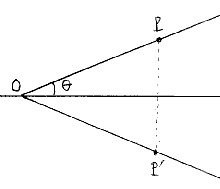
\includegraphics[scale=0.5]{angle.jpg}
  \]
  the angle $\angle POP'$ (where $O$ is the origin) is an angle of
  $-2\theta$ radians, so the effect of left multiplying by $H_0
  H_\theta$ is the same on $P$ as the effect of rotating $P$ by
  $-2\theta$ radians. So $H_0 H_\theta = R_{-2\theta}$, and we are
  done.
\end{proof}

In summary, we now have a complete understanding of the full
orthogonal group $\Orth(2)$. 


\begin{cor}
  $\Orth(2) = \{ R_\theta : \theta \in \R \} \cup \{ H_\theta :
  \theta \in \R\}$. 
\end{cor}

Another corollary of the theorem is that $\Orth(2)$ is generated by
$\SO(2)$ and $H_0$. (This is still true if $H_0$ is replaced by any
reflection.)

Now that we understand $\SO(2)$ and $\Orth(2)$, we return to the
dihedral groups $\D_n$ defined in a previous section. Recall that
\[
  \D_n = \{i, r, r^2, \dots, r^{n-1} \} \cup \{d, dr, dr^2, \dots,
  dr^{n-1} \}
\]
is the symmetry group of a regular $n$-gon. In the displayed
decomposition, the first set consists of rotations of the $n$-gon, and
the second consists of reflections of it. The reflection $d$ is the
one that fixes vertex $n$ of the $n$-gon.  

Note that all rotations and reflections of the $n$-gon must fix the
center point (centroid) of the $n$-gon. If we place the $n$-gon on the
euclidean plane $\R^2$ so that its centroid lies at the origin then
the rotations and reflections in $\D_n$ extend to rotations and
reflections of $\R^2$. (This requires further work to prove
rigorously, but it is intuitively clear.)

This means that the elements of the symmetry group $\D_n$ may be
represented by elements of the orthogonal group $\Orth(2)$; i.e., they
can be represented by $2 \times 2$ orthogonal matrices.  We choose to
place the $n$-gon in such a way that its $n$th vertex lies on the
positive $x$-axis. Then the extension of the symmetry $d$ is the
reflection $H_0$.  So the representation $f: \D_n \to \Orth(2)$ is
defined by
\[
  r \mapsto R_{2\pi/n}, \qquad d \mapsto H_0.
\]
The representation preserves products, in the sense that $f(ab) =
f(a)f(b)$, so the images displayed above determine the values of $f$
on every element of $\D_n$. Since $f$ is injective, it defines an
isomorphism of $\D_n$ onto the subgroup $\gen{R_{2\pi/n}, H_0}$ of
$\Orth(2)$ generated by $R_{2\pi/n}, H_0$.

So we can ``understand'' the dihedral group $\D_{n}$ by working with
matrices. 

What happens when we take the limit as $n$ approaches $\infty$? Well,
the regular $n$-gon approach a circle. The number of rotations, and
thus also the number of reflections, increases to infinity. So in some
sense it is fair to say that $\lim_{n \to \infty} \D_n =
\Orth(2)$. This enables another way to think of $\Orth(2)$ as a
symmetry group: $\Orth(2)$ is the symmetry group of a circle.  For
this reason, it is sometimes said that the group $\Orth(2)$ is the
``infinite dihedral group.''




\section*{Exercises}
\begin{problems}
\item Show that any matrix of the form $R_\theta$ must belong to
  $\SO(2)$, for any $\theta \in \R$.

\item Show that the origin is a fixed point for any rotation operator
  $\rho_\theta$.

\item Prove that the following identities follow from those in
  Corollary \ref{cor:rot-identities}.
  \begin{enumerate}
  \item $R_{\theta_1} R_{\theta_2} = R_{\theta_1+\theta_2}$
    and $(R_\theta)^{-1} = R_{-\theta}$, for all $\theta, \theta_1,
    \theta_2 \in \R$.
  \item $R_{\theta_1} R_{\theta_2} = R_{\theta_2} R_{\theta_1}$ for
    all $\theta_1, \theta_2 \in \R$.
  \end{enumerate}

\item Use the results of the preceding exercise to give a conceptual
  derivation of the addition formulas for sine and cosine.

\item Give a different proof of Theorem \ref{thm:rotation}, by showing
  that the angle between $X$ and $\rho_\theta(X)$ is equal to
  $\theta$, for any $0 \ne X\in \R^2$. [Hint: Recall that the angle
    between two vectors in $\R^2$ is determined by dot products.]

\item Show that the product of any two reflection matrices in
  $\Orth(2)$ must be a rotation matrix.

\item 
  \begin{enumerate}
  \item Show that $H_\theta = R_{2\theta} H_0$.
  \item Show that $R_{2\theta} H_0 R_{2\theta} = H_0$. What formula
    holding for dihedral groups is this similar to?
  \end{enumerate}

\item 
  \begin{enumerate}
  \item Argue that the composite of a reflection and a rotation (in
    either order) must be a reflection.
  \item Show that $H_{\theta_1} R_{\theta_2}$ must be some reflection
    matrix, i.e., some $H_{\theta_3}$. Figure out what reflection
    matrix it is; i.e., figure out how to express $\theta_3$ in terms
    of $\theta_1, \theta_2$. Justify your answer.
  \end{enumerate}

\end{problems}




\newpage
\section{Matrix groups over other fields}\noindent
Most of the basic theory of matrices, and indeed all of linear
algebra, which is usually developed initially over the field $\R$ of
real numbers, generalizes to any field\index{field} $F$. In this
generalization, the vector space $\R^n$ of $n$-tuples of real numbers
is replaced by the vector space $F^n$ of $n$-tuples over $F$, and
matrices with entries from $\R$ are replaced by matrices with entries
from $F$.

\begin{examples}
Here are some important examples of matrix groups over an arbitrary
field $F$. The field $F$ could be $\Q, \C$, or even a finite Galois
field $\F_p$.

1. The \emph{general linear group}\index{general~linear~group}
$\GL(n,F) = \GL_n(F)$\index{GL@$\GL_n(F)$} is the group consisting of
all $n \times n$ nonsingular matrices with entries from the field
$F$. In symbols,
\[
  \GL_n(F) = \{ n \times n \text{ matrices } A : \det A \ne 0\}.
\]
The group $\GL_n(F)$ is finite if the field $F$ is finite. 

2. The \emph{special linear group}\index{special~linear~group} $\SL(n,
F) = \SL_n(F)$\index{SL@$\SL_n(F)$} is the group consisting of all $n
\times n$ matrices of determinant equal to $1$. In symbols,
\[
  \SL_n(F) = \{ A \in \GL_n(F) : \det A = 1 \}.
\]
By definition, we have an inclusion $\SL_n(F) \subset
\GL_n(F)$. Again, this is a finite group if the field $F$ is finite.
\end{examples}

It is also possible to define orthogonal
groups\index{orthogonal~group} over fields other than $\R$, but there
are technicalities that we do not want to face at the moment.

When one allows the field $F$ to be the field of complex numbers, we
of course have $\GL_n(\C)$ and $\SL_n(\C)$ as above, but two important
extra examples appear, as follows.

\begin{examples}
1. The \emph{unitary group}\index{unitary~group} $\U(n) =
\U_n(\C)$\index{U@$\U(n)$} is the group consisting of all $n \times
n$ unitary matrices. A square matrix $A$ with complex entries is
\emph{unitary} if $A^{-1} = A^*$, where $A^* =
\overline{A}^\transpose$. The matrix $A^*$ is called the
\emph{conjugate transpose} of $A$. It is obtained by first taking the
complex conjugate of each entry of $A$ to get the matrix
$\overline{A}$, and then taking the transpose.

2. The \emph{special unitary group}\index{special~unitary~group}
$\SU(n) = \SU_n(\C)$\index{SU@$\SU(n)$} is the group consisting of all
$n \times n$ special unitary matrices. A square matrix $A$ with
complex entries is \emph{special unitary} if it is unitary and has
determinant equal to 1.
\end{examples}

Unitary groups play a fundamental role in mathematical physics. 


\begin{example}
Many basic properties of matrices work for matrices with entries from
an arbitrary ring $R$. This observation leads to many more new
examples of matrix groups.  For instance, the group
\[
  \SL(n,\Z) = \SL_n(\Z) = \{n \times n \text{ matrices $A$ with integer
    entries} \mid \det A = 1 \}
\]
makes sense and has been studied extensively. It is an example of an
\emph{arithmetic group}\index{arithmetic~group}. Arithmetic groups
have connections to number theory and lattice theory.
\end{example}

Lattice theory has recently been applied to invent new public-key
cryptosystems.



\section*{Exercises}\noindent

\begin{problems}
\item 
  \begin{enumerate}
  \item List all the matrices in $\GL_2(\F_2)$.
  \item List all the matrices in $\SL_2(\F_2)$.
  \end{enumerate}
 

\item Use counting principles to compute $|\GL_2(\F_p)|$. 

\item Use counting principles to compute $|\SL_2(\F_p)|$. 

\item Let $F$ be any field. Let $G$ be the set of all matrices of the
    form $E(t) = \begin{bmatrix} 1&t\\ 0&1
  \end{bmatrix}$, where $t \in F$. 
  \begin{enumerate}
  \item Show that $E(s) E(t) = E(s+t)$ for any
    $s,t \in F$.
  \item Show that $E(t)^{-1} = E(-t)$ for any $t \in F$.
  \item Prove that the set $G$ is a matrix group. (You have to show it
    is a nonempty set of matrices that is closed under products and
    inverses.)
  \end{enumerate}

\item Let $G$ be the set of all block matrices of the form
  $\begin{bmatrix} A&B\\ 0&C \end{bmatrix}$ with $A,B, C$ all $2\times
  2$ matrices over a field $F$ such that $\det(AC) \ne 0$. Verify that
  $G$ is a matrix group.

\item Show that $\SU(1) = \SU_1(\C)$ is isomorphic to the
  multiplicative group $\{ e^{i\theta} \mid \theta \in \R\}$ of points
  on the unit circle, regarded as a subgroup of $\C^\times$.

\end{problems}

\end{document}


\chapter{Abstract Groups}
\documentclass[11pt]{article}
\usepackage[nohead,margin=1.50in]{geometry} %set margins
\usepackage{amsmath,amssymb,amsthm,pdiag} %AMS packages for math stuff
\usepackage{multicol} % for use in HW section
\usepackage{enumitem}
  \setlist{topsep=1pt,itemsep=0pt,parsep=1pt}
  \setenumerate[1]{label=(\alph*)}

\newenvironment{problems}
{
 \begin{enumerate}[topsep=1pt,itemsep=0pt,parsep=2pt,leftmargin=0.6cm,%
 label={\arabic*.}, ref=\arabic*] \small
}
{
 \end{enumerate}
}

%%% Define some theorem and example environments. The starred versions
%%% are un-numbered and the unstarred versions are numbered.
\newtheoremstyle{plain}
  {\topsep}   % ABOVESPACE
  {\topsep}   % BELOWSPACE
  {\slshape}  % BODYFONT
  {0pt}       % INDENT (empty value is the same as 0pt)
  {\bfseries} % HEADFONT
  {.}         % HEADPUNCT
  {5pt plus 1pt minus 1pt} % HEADSPACE
  {}          % CUSTOM-HEAD-SPEC

\swapnumbers
\newtheorem{thm}{Theorem}[section]
\newtheorem{lem}[thm]{Lemma}
\newtheorem{prop}[thm]{Proposition}
\newtheorem{cor}[thm]{Corollary}
\newtheorem*{thm*}{Theorem}
\newtheorem*{lem*}{Lemma}
\newtheorem*{prop*}{Proposition}
\newtheorem*{cor*}{Corollary}

\theoremstyle{definition}
\newtheorem{defn}[thm]{Definition}
\newtheorem{example}[thm]{Example}
\newtheorem{examples}[thm]{Examples}
\newtheorem{rmk}[thm]{Remark}
\newtheorem{rmks}[thm]{Remarks}
\newtheorem{conv}[thm]{Convention}
\newtheorem*{defn*}{Definition}
\newtheorem*{example*}{Example}
\newtheorem*{examples*}{Examples}
\newtheorem*{rmk*}{Remark}
\newtheorem{rmks*}{Remarks}
\newtheorem*{conv*}{Convention}


%%% Define some convenient abbreviations for common mathematical
%%% notations.
\newcommand{\R}{\mathbb{R}} % use \R for the real numbers
\newcommand{\C}{\mathbb{C}} % use \C for the complex numbers
\newcommand{\Z}{\mathbb{Z}} % use \Z for the integers
\newcommand{\Q}{\mathbb{Q}} % use \Q for the rationals
\newcommand{\N}{\mathbb{N}} % use \N for the natural numbers
\newcommand{\F}{{\mathbb F}}
\newcommand{\compose}{\circ} % functional composition
\newcommand{\gen}[1]{\langle #1 \rangle}
\newcommand{\End}{\operatorname{End}}
\newcommand{\GL}{\mathrm{GL}}
\newcommand{\SL}{\mathrm{SL}}
\renewcommand{\O}{\mathrm{O}}
\newcommand{\SO}{\mathrm{SO}}
\newcommand{\U}{\mathrm{U}}
\newcommand{\SU}{\mathrm{SU}}
\newcommand{\g}{\mathfrak{g}}
\newcommand{\transpose}{\mathsf{T}}
\newcommand{\B}{\mathcal{B}}
\newcommand{\Rep}{\operatorname{Rep}}
\newcommand{\Mat}{\operatorname{Mat}}
\newcommand{\inner}[2]{\langle #1, #2 \rangle}
\newcommand{\sgn}{\operatorname{sgn}}
\newcommand{\n}{\underline{\mathbf{n}}}
\newcommand{\Sym}{\mathbb{S}}
\newcommand{\Alt}{\mathbb{A}}
\newcommand{\D}{\mathbb{D}}
\newenvironment{perm}[2]{\left(\begin{smallmatrix}#1 \\ #2}{\end{smallmatrix}\right)}
\newcommand{\lcm}{\operatorname{lcm}}
\newcommand{\res}{\operatorname{res}}

\allowdisplaybreaks
\parskip=2pt



%\title{Document Title}
%\author{author's name}

\begin{document}%\maketitle
\setcounter{section}{16}

\section{Abstract groups}\noindent
The axiomatic definition of abstract group\index{abstract~group} is
based on special classes of examples of groups, such as permutation
groups and matrix groups.  Those examples share some common features:
closure under products and inverses, associativity, and identity. In
the definition we are about to give, closure under products is
implicit in the definition of binary operation, while closure under
inverses is an axiom.

We start with the concept of a binary
operation\index{binary~operation} on a set. Intuitively, a binary
operation is a \emph{law of combination} which combines two elements
of a set to produce another element of the set. Ordinary addition and
multiplication are canonical examples.

\begin{defn}
Let $S$ be any given set. Any function from $S \times S$ to $S$ is
called a {\em binary operation} or \emph{law of combination} on the
set $S$. If $f$ is a binary operation then tradition demands that we
write $x\,f\,y$ for the value\footnote{Writing a function between its
  arguments is called {\em infix} notation in computer science.} at
the input pair $(x,y)$ instead of the usual $f(x,y)$.
\end{defn}

In this context the word \emph{binary} refers to the fact that the
function depends on two input variables. By the same token, a
\emph{unary operation} on the set $S$ would be a function from $S$ to
itself. For example, the function that sends each integer to its
negative is a unary operation on the set $\Z$ of integers.

\begin{examples}
1. Addition ($+$) is a binary operation on any of the usual number
sets $\N$, $\Z$, $\Q$, $\R$, $\C$. Multiplication ($\cdot$) is another
binary operation on any of the sets $\N$, $\Z$, $\Q$, $\R$, $\C$.

2. Matrix multiplication is a binary operation on the set
$\text{Mat}_n(F)$ of all $n \times n$ matrices with entries in a given
field $F$.

3. Composition of functions is a binary operation on the set $\Sym_n$
of permutations of $\underline{\mathbf{n}} = \{1, \dots, n\}$.


4. More generally, composition of functions is a binary operation on
the set $S^S$ of all self-maps $S \to S$ of \emph{any} set $S$.

5. Here is a binary operation $\#$ on the finite set $S=\{a,b,c,d\}$
which is defined by means of a ``multiplication'' table as follows:
$$
\begin{array}{|c|cccc|}\hline
\#& a&b&c&d\\ \hline
a & a&a&d&d\\
b & b&b&c&c\\
c & a&d&b&c\\
d & b&c&a&d\\
\hline
\end{array}
$$ This table defines a law of combination for pairs of elements of
$S$. For instance, it says that $a\#c = d$ and $c\#b = d$. For finite
sets $S$, we can always define a binary operation (law of combination)
on $S$ by a table.
\end{examples}



It is important to realize that closure under products is built in to
the definition of a binary operation: to say that $*$ is a binary
operation on $S$ \emph{means} that $S$ is closed under $*$, since all the
values $x*y$ must fall again within $S$, for any $x,y \in S$. This is
just another way of saying that $*$ is a function mapping $S \times S
\to S$.



\begin{defn}
\index{definition~of~group}\index{group~axioms}\label{def:group}
A {\em group} is a set $G$ along with a given binary operation $*$
on $G$, such that the following three axioms hold:
\begin{enumerate}
\item[(G1)] The operation $*$ is {\em associative}: $(a*b)*c =
  a*(b*c)$ for all $a,b,c \in G$.

\item[(G2)] There is an {\em identity} element $e \in G$ satisfying:
  $e*a = a = a*e$ for all $a\in G$.

\item[(G3)] Each $a \in G$ has an {\em inverse} in $G$: given $a \in
  G$ there exists some $a' \in G$ such that $a*a' = a'*a = e$.
\end{enumerate}
\end{defn}


Note that closure under $*$ is implicit in this definition, since $*$
is a binary operation on $G$. Moreover, closure under inverses is the
content of axiom (G3).


When describing a group we should specify not only the set $G$ but
also the binary operation $*$ on $G$, since a given set can have many
different binary operations defined on it. People often use a notation
such as $(G,*)$ to denote a group. If the binary operation $*$ is
implied by context, then we often just write $G$ for simplicity.


\begin{defn}\index{abelian~group}
An {\em abelian}\footnote{In honor of Niels Henrik Abel
  (1802--1829).} group is any group $(G,*)$ in which the commutative
law holds: $a*b=b*a$, for all $a,b\in G$.
\end{defn}

As we have seen, matrix and permutation groups are usually not
abelian, because matrix multiplication and functional composition are
usually not commutative. 


\begin{thm}[Basic properties]\label{gpprop} 
Let $(G,*)$ be any group, with binary operation $*$, and let $a,d,x,y
\in G$.
\begin{enumerate}
\item The identity element $e \in G$ in axiom {\rm(G2)} is unique.

\item The inverse of any $a \in G$ in axiom {\rm(G3)} is unique.

\item The equation $a*x=a*y$ implies that
  $x=y$.  (This is called {\em left cancellation}.)

\item The equation $x*a=y*a$ implies that
  $x=y$.  (This is called {\em right cancellation}.)

\item Each of the equations $a*x=b$, $x*a = b$ ($a,b\in G$) has a
  unique solution $x \in G$.

\item\index{inverse~of~a~product} The inverse of a product is the
  product of the inverses in reverse order.
\end{enumerate}
\end{thm}


\begin{proof} 
(a) Suppose that $e$, $f$ are identity elements of $G$. Then by
  axiom (G2) we have $e*a=a$ and $a=a*f$ for all $a\in G$. In
  particular, taking $a=f$ in the first equality and $a=e$ in the
  second, we get $e*f=f$ and $e=e*f$. Hence $e=f$. This proves
  uniqueness of identity.

(b) Suppose that $b$, $c$ are both inverses of a given $a \in G$. Then
  $a*b=e=b*a$ and $a*c=e=c*a$ by axiom (G3). By the associative law
  (G1) we have $c*(a*b) = (c*a)*b$, so $c*e=e*b$, so $c=b$ by
  (G2). This proves uniqueness of inverses.

(c) Suppose $a*x=a*y$. Then $a'*(a*x) = a'*(a*y)$ where $a'$ is the
  inverse of $a$. By (G1) this implies that $(a'*a)*x = (a'*a)*y$, so
  by (G3) we have $e*x = e*y$, which implies by (G2) that $x=y$.


(d) This is proved similarly to (c), except we multiply by the
  inverse $a'$ on the right instead of on the left.

(e) Suppose that $a*x=b$. Then by left multiplication by the inverse
  $a'$ of $a$ we have $a'*(a*x) = a'*b$, so by (G1) we have $(a'*a)*x
  = a'*b$. Thus by (G3) we have $e*x = a'*b$, so by (G2) we obtain $x
  = a'*b$. This is the unique solution.  This proves the first
  claim. The other claim is proved similarly, using right
  multiplication instead of left multiplication.

(f) Given two elements $a,b$ of $G$ let their respective inverses be
  $a',b'$. Then by axiom (G3) we have $a*a'=e$, $b*b'=e$. Thus 
  \[
    (a*b)*(b'*a') = a*(b*b')*a' = (a*e)*a' = a*a' = e,
  \]
  where we used generalized associativity for the first equality. Let
  $z$ be the inverse of $a*b$. Then $(a*b)*z = e$ by (G3). So $(a*b)*z
  = (a*b)*(b'*a')$. By left cancellation we obtain $z = b'*a'$, i.e.,
  the inverse of $a*b$ is $b'*a'$. This proves the statement for
  products of length two, and it easily extends to products of more
  than two elements, by induction on the length of the product.
\end{proof}



\subsection*{Additive versus multiplicative notation}
\index{additive~notation}\index{multiplicative~notation}%
If the binary operation $*$ is written as addition ($+$) or
multiplication (\,$\cdot$\,) then the group is known as an \emph{additive}
group or a \emph{multiplicative} group, respectively.

If $(G,+)$ is an additive group, it is customary to denote the
identity element by the symbol $0$ and the inverse of $a$ by the
symbol $-a$.  In this case the group axioms take the following form:

(G1)\quad $(a+b)+c = a+(b+c)$; 

(G2)\quad $0+a=a=a+0$; 

(G3)\quad $a+(-a) = 0 = (-a)+a$.

\noindent
It is customary to use the additive notation for a group {\em only for
  abelian groups} and we shall follow that convention in this course.

If $(G, \cdot)$ is a multiplicative group, it is customary to
abbreviate products $a \cdot b$ by $ab$. In this case we usually
denote the identity element by the symbol $1$ and the inverse of $a$
by the symbol $a^{-1}$. Then the group axioms take the form:

(G1)\quad $(ab)c = a(bc)$; 

(G2)\quad $1a=a=a1$; 

(G3)\quad $aa^{-1} = 1 = a^{-1}a$.

The default notation for the group operation is multiplicative
notation, but additive groups appear frequently as well.



\begin{examples} \label{ex}
(a) Any permutation group is a group. Any matrix group is a group. 

(b) The dihedral group $\D_n$ is a group. All symmetry groups are
  groups.

(c) The \emph{abstract cyclic group} is the multiplicative group $C_n$
  generated by a symbol $x$ subject to the relation $x^n = 1$. As a
  set, $C_n = \{1, x, x^2 \dots, x^{n-1}\}$, so $|C_n| = n$.

(d) Any vector space\index{vector~space} $V$ gives an additive abelian
  group $(V,+)$ under vector addition. The identity element is the
  zero vector $\mathbf{0}$ in $V$ and the additive inverse of a vector
  $\mathbf{v} \in V$ is the vector $-\mathbf{v}$. In particular,
  $(\R^n, +)$ is an example of such a group, and more generally we
  have the group $(F^n, +)$ where $F$ is any field.

(e) Any ring\index{ring} $R$ (commutative or not) contains \emph{two}
  groups. One is the additive abelian group $(R,+)$, in which $0$ is
  the additive identity and the inverse of $a$ is written as $-a$. In
  particular, $(\Z, +)$, $(\Q, +)$, $(\R,+)$, $(\C, +)$ are all
  additive abelian groups. Also, $(\Z_n, +)$ is an additive abelian
  group, for any positive integer $n$.

(f) Recall that $R^\times = R^*$\index{R@$R^\times$} is the set of
  units\footnote{A \emph{unit} is an invertible element.} in a given
  ring $R$. The second group in the ring $R$ is the
  \emph{multiplicative group of units} in $R$, i.e., the group
  $(R^\times, \cdot)$ or just $R^\times$ for short.  In particular,
  for any positive integer $n$, we have the multiplicative group
  $\Z_n^\times$ of units in the ring $\Z_n$. The abelian group
  $\Z_n^\times$ is of extreme importance for modern cyptography.

(g) Let $F$ be any field\index{field}. Then by definition $F^\times =
  F-\{0\}$, the set of all nonzero elements of $F$, since every
  nonzero element of a field is invertible. So the previous example
  gives in this case the group $(F^\times, \cdot) = (F-\{0\}, \cdot)$,
  which is called the {\em multiplicative group of the field} $F$.

(h) The {\em trivial group}\index{trivial~group} is the set $\{e\}$
  consisting of only one element, with $e*e=e$.
\end{examples}

The number of elements of a group is called its
\emph{order}.

\begin{defn}\index{order!of~a~group}
  Let $(G,*)$ be a group. The {\em order} of the group is the
  cardinality $|G|$ of the set $G$. If the set $G$ is an infinite set
  then we often write $|G| = \infty$ and call $G$ an infinite group,
  otherwise $G$ is a finite group.
\end{defn}

The word \emph{order} is also used in group theory in another way, as
follows, when speaking about an element of a group.

\begin{defn}\label{def:order-elt}\index{order!of~an~element}
  Let $a \in G$ where $(G,*)$ is a group.  The {\em order} of $a$ is
  the least positive integer $r$ such that $a$ combined with itself
  $r$ times yields the identity element $e$.  If no such $r$ exists,
  then the order is defined to be $\infty$.
\end{defn}

In any group, the order of the identity element is always 1.  Since
the word \emph{order} has two different meanings within group theory,
we always have to determine its usage from the context.

\begin{lem}\label{lem:inverse-if-finite}
  If $a$ is an element of order $r$ in a group $(G,*)$, then the
  inverse of $a$ is equal to $a* \cdots *a$ ($r-1$ factors) obtained
  by combining $a$ with itself $r-1$ times.
\end{lem}

\begin{proof}
  Let $b$ be equal to $a* \cdots *a$ ($r-1$ factors). Then it is clear
  that $a*b = e = b*a$. It follows from uniqueness of inverses that
  $b$ equals the inverse of $a$.
\end{proof}



Now we discuss \emph{laws of exponents}\index{laws~of~exponents} in
groups. We need to distinguish between multiplicative and additive
groups, which use different notation.  If $a$ is an element of a
multiplicative group, then we define $a^n$ to be $aa\cdots a$ ($n$
times repeated) for any positive integer $n$, we define $a^0 = 1$, and
we define $a^{-n} = (a^{-1})^n$.  Note that $(a^n)^{-1} =
a^{-n}$. Moreover, we have
\[
  a^m\,a^n = a^{m+n}, \qquad (a^m)^n = a^{mn}
\]
for any $m,n \in \Z$.

In an additive group we have to use a different notation. In this case we
define $n a$ to be $a+a+\cdots+a$ ($n$ summands) for any positive
integer $n$, we define $0 a = 0$, and we define $(-n) a = n(-a)$. 
Note that $-(na) = (-n)a$.  Moreover, 
\[
  ma + na = (m+n)a, \qquad n(ma) = (nm)a
\]
for any $m,n \in \Z$. In an additive group, ``powers'' are written as
multiples, because in ordinary arithmetic repeated addition is written
as a multiple while repeated multiplication is written as a power.


\begin{rmk}
We can rephrase Definition \ref{def:order-elt} in terms these
notations as follows.  In a multiplicative group the order of $a$ is
the least positive integer $r$ such that $a^r = 1$. In the additive
case the order of $a$ is the least positive integer $r$ such that $ra
= 0$.
\end{rmk}

Now we define the important notion of isomorphism of groups. 

\begin{defn}
  Let $(G,*)$ and $(H,\#)$ be given groups. An \emph{isomorphism} of
  $G$ onto $H$ is any bijection $f \colon G \to H$ such that $f(a*b) =
  f(a)\#f(b)$ for all $a,b \in G$. Whenever such an $f$ exists then we
  say that $G$ is \emph{isomorphic} to $H$, and write $G \cong H$ or
  $G \simeq H$ (interchangeably).
\end{defn}

So an isomorphism is a bijective mapping from one group to the other
which matches up products in the two groups. If one group is an
additive group and the other a multiplicative group then this means
that sums get matched with products.

If two groups are isomorphic then {\em they are essentially the same
  group}, except for the form of their elements. In particular,
isomorphic groups must have the same structural properties (i.e, they
have same order, the same number of subgroups, etc). The following is
easy to check.


\begin{thm}\label{thm:iso}\index{isomorphism}
  Isomorphism of groups is an equivalence relation on the class of
  groups: it is reflexive, symmetric, and transitive.
\end{thm}

\begin{example}\index{R@$\R^+$}
It is easy to check that the set $(\R^+, \cdot)$ of all positive real
numbers is a group under multiplication. We claim that the
multiplicative group $(\R^+, \cdot)$ is isomorphic to the additive
group $(\R, +)$ of real numbers. The isomorphism is given by the
natural logarithm function $x \mapsto \ln x$. We know this function is
invertible (its inverse is the exponential function $x \mapsto e^x$)
so it is a bijection of $\R^+$ onto $\R$. Furthermore, the equation
$\ln(ab) = \ln(a) + \ln(b)$ says that products in $\R^+$ match up with
sums in $\R$, so the function $\ln$ is indeed a group isomorphism, as
claimed.
\end{example}


If a group $(G,*)$ is finite then it may be described by giving its
complete multiplication table. (Replace multiplcation by addition if
it is an additive group.) For instance, the addition table of
$(\Z_4,+)$ and the multiplication table of the cyclic group $G =
\gen{\alpha}$ generated by a $4$-cycle $\alpha$ are displayed in the
tables below
\[
\begin{array}{|c|cccc|} \hline
+&0&1&2&3\\ \hline 
0&0&1&2&3\\ 1&1&2&3&0\\ 
2&2&3&0&1\\ 3&3&0&1&2\\ \hline
\end{array}
\qquad \qquad
\begin{array}{|c|cccc|} \hline
\cdot&1&\alpha&\alpha^2&\alpha^3\\ \hline 
1&1&\alpha&\alpha^2&\alpha^3\\ \alpha&\alpha&\alpha^2&\alpha^3&1\\ 
\alpha^2&\alpha^2&\alpha^3&1&\alpha\\ \alpha^3&\alpha^3&1&\alpha&\alpha^2\\ 
\hline
\end{array}
\]
where we write the numbers $0, 1, 2, 3$ as a shorthand for the
corresponding residue classes $[0], [1], [2], [3]$ in $\Z_4$. Note
that the correspondence 
\[
  [0] \to 1 = \alpha^0, \quad [1] \to \alpha = \alpha^1, \quad [2] \to
  \alpha^2, \quad [3] \to \alpha^3
\] 
defines an isomorphism between the two groups. In a more succinct
notation, the isomorphism is defined by $f([x]) = \alpha^x$ for $x =
0,1,2,3$.


The multiplication table of a finite group has the property that the
elements in any row of the table form a permutation of the elements of
any other row. The same is true of the columns of the table. In
particular, no element appears twice in any row or any column. You
should be able to show how these claims follow from the group axioms.

Consider a group of order $2$. Assume that its binary operation is
written multiplicatively, so $G = \{1, a\}$ as a set, where $1$ is the
identity element and $a \ne 1$ (else the group would have order
$1$). Then necessarily $a^2=1$, because $a^2=a$ implies $a=1$. So the
group multiplication table must look like the one on the left below:
\[
\begin{array}{|c|cc|} \hline
\cdot&1&a\\ \hline 
1&1&a\\
a&a&1\\
\hline
\end{array}
\qquad \qquad
\begin{array}{|c|cc|} \hline
+&0&1\\ \hline 
0&0&1\\
1&1&0\\
\hline
\end{array}
\]
The table on the right is the addition table for the additive group
$(\Z_2,+)$. It should be clear that the two groups are
isomorphic. This analysis shows that any group of two elements must be
isomorphic to $\Z_2$. This argument can be extended to prove that any
group of three elements must be isomorphic to $\Z_3$.


%\newpage
\section*{Exercises}
\begin{problems}\small

\item Explain your reasoning for:
\begin{enumerate}
\item Is $\N = \{1,2,3,\dots \}$ a group under addition? If we
  include $0$ is it a group?
\item Is $\N= \{1,2,3,\dots \}$ a group under multiplication?
\item Is the set $\Z$ of integers a group under addition? 
\item Is $\Z$ a group under multiplication? 
\item Is $\Z-\{0\}$ a group under multiplication? 
\end{enumerate}


\item What is wrong with writing $\frac{a}{b}$ for $ab^{-1}$ in a
  (nonabelian) multiplicative group? If you think there is nothing
  wrong with it, then how will you write $b^{-1} a$ when $ab^{-1} \ne
  b^{-1}a$?

\item Prove that any group of three elements must be isomorphic to
  the additive group $\Z_3$ by analyzing its multiplication table.

\item Suppose that $G = \{1,a,b,c\}$ is a multiplicative group of four
  elements in which $1$ is the identity element. By analyzing the
  possible multiplication tables, prove that $G$ is isomorphic to
  either $(Z_4,+)$ or to a group in which $a^2=b^2=c^2=1$. (The latter
  group is called the Klein 4-group\index{Klein~four~group}.)

\item List the elements in the following multiplicative groups:

(a) $(\Z^\times,\cdot)$,\qquad
(b) $(\Z_6^\times, \cdot)$,\qquad
(c) $(\Z_8^\times, \cdot)$,\qquad
(d) $(\Z_{15}^\times, \cdot)$.

\item Give multiplication tables for the groups in the previous
  problem.

\item Prove that $|\Z_n^\times| = \varphi(n)$, where $\varphi(n)$ is
  \emph{Euler's phi-function} from number theory.

\item Prove that the elements in any row of the group multiplication
  table of a finite group $G$ form a permutation of the elements of
  the first row. Then do the same for columns. 

\item In this problem, we write $\Z_n$ for the additive group
  $(\Z_n,+)$. Find the order of:

(a) 1 in $\Z_7$, \qquad 
(b) 2 in $\Z_7$, \qquad 
(c) 1 in $\Z_{10}$, \qquad 
(d) 2 in $\Z_{10}$, \qquad 
(e) 3 in $\Z_{10}$.

\item In this problem, we write $\Z_n$ for the additive group
  $(\Z_n,+)$. Find the order of any $a \in \Z_n$ and prove your
  answer.

\item In this problem, we write $\Z_n^\times$ for the multiplicative
  group $(\Z_n^\times, \cdot)$ of units. Find the orders of:

(a) $1,2,3,4,5,6$ in $\Z_7^\times$, \qquad
(b) $1,2,4,5,7,8$ in $\Z_{9}^\times$, \qquad
(c) $1,3,7,9$ in $\Z_{10}^\times$.


\item\label{prob:circle-gp} (The circle group) Let $S^1$ be the set of
  all points on the usual unit circle in the plane $\R^2$.  Show that
  $S^1$ is a group under the law of combination given by
  \[
    (\cos \theta, \sin \theta) * (\cos \theta', \sin \theta') = (\cos
    (\theta + \theta'), \sin(\theta + \theta')).
  \] 
  Be sure to give a formula for the inverse of elements of this group,
  and prove that they really are inverses. 

\item Show that the circle group of the previous problem is isomorphic
  to the matrix group $\SO(2)$.


\item Find an isomorphism of the multiplicative group $\Z^\times$ onto
  the additive group $\Z_2$.



\item Consider the set $G$ of all $2 \times 2$ real matrices of the
  form $[\begin{smallmatrix} a&-b\\b&a \end{smallmatrix}]$.
  \begin{enumerate}
  \item Show that $G$ is a group under ordinary matrix addition, and
    find an isomorphism from the additive group $(\C, +)$ onto $G$.
  \item Now let $G'$ be the subset of $G$ consisting of all elements
    of $G$ except the zero matrix. Show that $G'$ is a group under
    ordinary matrix multiplication. 
  \item Find an isomorphism from the multiplicative group $(\C^\times,
    \cdot)$ onto $G'$.
  \end{enumerate}

\item Prove part (f) of Theorem \ref{gpprop} using right
cancellation instead of left cancellation.


\item Prove that isomorphism of groups is an equivalence relation
on the class of groups (Theorem \ref{thm:iso}).


\item Prove that if $G$ is a group in which every element (except the
  identity) has order 2 then $G$ must be abelian.

\item \label{prob:monoids} (Monoids) A \emph{monoid} is a set $M$
  along with a binary operation $*: M \times M \to M$ such that $*$ is
  associative and there is an identity element $e \in M$. Show that
  $(\N, +)$ and $(\Z, \cdot)$ are monoids but not groups.


  

\item Show that a set $R$ with two binary operations $+, \cdot$ is a
  ring\index{ring} if and only if the following three properties hold:
  \begin{enumerate}
  \item $(R,+)$ is an additive abelian group. Denote its identity
    element by $0$.
  \item $(R, \cdot)$ is a multiplicative monoid (see Problem
    \ref{prob:monoids} for the definition of monoid). Denote its
    identity element by $1$.
  \item Addition and multiplication are connected by the distributive
    laws: $a(b+c) = ab+ac$ and $(b+c)a = ba+ca$, for all $a,b,c \in
    R$.
  \end{enumerate}
  Thus, one could take the three properties as the definition of ring.



\item Show that a set $F$ with two binary operations $+, \cdot$ is a
  field\index{field} if and only if the following four properties hold:
  \begin{enumerate}
  \item $(F,+)$ is an additive abelian group. Denote its identity
    element by $0$.
  \item $(F-\{0\}, \cdot)$ is a multiplicative abelian group. Denote
    its identity element by $1$.
  \item $1 \ne 0$.
  \item Addition and multiplication are connected by the distributive
    law: $a(b+c) = ab+ac$, for all $a,b,c \in F$.
  \end{enumerate}
  Thus, one could take the four properties as the definition of field.

\end{problems}

 

\newpage
\section{Subgroups}\noindent
Finding subgroups inside known groups is an important way of finding
new examples of groups. 

\begin{defn}\index{subgroup}
  Let $(G,*)$ be a group. A subset $H$ of $G$ is called a
  \emph{subgroup} of $G$ if $(H,*)$ is a group in its own right. We
  write $H<G$ (or $H \le G$ interchangeably) to denote that $H$ is a
  subgroup of $G$. A subgroup $H$ is a \emph{proper} subgroup of $G$
  (written as $H \lneqq G$) if $H \ne G$.
\end{defn}


By definition, permutation groups are subgroups of some $\Sym_n$ and
matrix groups are subgroups of some $\GL_n(F)$, where $F$ is a field.
So we have already seen many examples of subgroups.

Note that every group is regarded as a subgroup of itself. (So in the
above notation, writing $G<G$ is perfectly valid.) In any group the
subset consisting solely of the identity element is always a subgroup;
this subgroup is called the \emph{trivial} subgroup.

In order for a given subset $H$ of a group $G$ to be a subgroup, it is
clearly necessary that the binary operation $*: G \times G \to G$
restricts to a binary operation $*: H \times H \to H$. This is just
another way of saying that $H$ must be closed under products.

The following theorem covers both the multiplicative and additive
cases together. In the latter case, you should read ``sum'' for
``product'' in the theorem, because $a*b = a+b$ when the operation $*$
is equal to $+$. 


\begin{thm}[The subgroup criterion]\index{subgroup~criterion}
  Let $H$ be a nonempty subset of a given group $(G,*)$.  Then $H$ is
  a subgroup of $G$ if and only if $H$ is closed under products and
  inverses. (Closure under products means that $a*b \in H$ whenever
  $a,b \in H$, and closure under inverses means that $H$ contains the
  inverse of each of its elements.)
\end{thm}

\begin{proof}
  ($\implies$) Suppose that $H$ is a subgroup of $G$. Then the fact
  that $H$ is a group in its own right means that when we restrict the
  operation $*\colon G \times G \to G$ to the subset $H \times H$, it
  induces a binary operation $*\colon H \times H \to H$. This is
  equivalent to saying that $H$ is closed under products. Also, the
  fact that axiom (G3) holds for $H$ means that each $a \in H$ has an
  inverse $a'$ in $H$; that must also be its inverse in $G$ since
  inverses in $G$ are unique.  This implies that $H$ is closed under
  inverses.

  ($\impliedby$) Suppose that $H$ is a nonempty subset of $G$ which is
  closed under products and inverses. Then the restriction of $*$ to
  $H \times H$ maps into $H$, and thus defines a binary operation on
  $H$. Axiom (G1) is automatic in $H$ since it holds in the bigger set
  $G$. Axiom (G3) for $H$ is just closure under inverses, which is
  true by assumption. Finally, closure under products and inverses
  implies that the identity $e$ is in the set $H$, since there must be
  some $a \in H$ (because $H$ is nonempty) and then its inverse $a'$
  is in $H$ and thus $a*a' = e \in H$ by closure under products. This
  proves axiom (G2) for $H$.
\end{proof}

The following result is a slightly simplified version of the subgroup
criterion. 


\begin{thm}[Simplified subgroup criterion]
  Let $H$ be a nonempty subset of a given group $G$, and write $b'$
  for the inverse of $b \in G$.  Then $H$ is a subgroup of $G$ if and
  only if $a*b' \in H$ for all $a,b \in H$.
\end{thm}

\begin{proof} 
($\implies$) Suppose $H<G$. Then by the subgroup criterion, for any
  $a,b \in H$ it follows that $b' \in H$ and hence $a*b' \in H$.

($\impliedby$) For the converse, suppose that $H$ is a nonempty
  subset and $a*b' \in H$ for all $a,b \in H$. Since $H$ is non-empty
  there is at least one element $c \in H$. Hence $c*c' \in H$, so the
  identity $e \in H$.  Hence $b' = e*b' \in H$ for every $b\in H$,
  proving that $H$ is closed under inverses. Finally, if $a,b$ are any
  elements of $H$, then $b'\in H$ as we have just shown. Note that
  $(b')' = b$, so $b = d'$ where $d = b' \in H$. Hence the product
  $a*b = a*d'$ must be an element of $H$. This shows that $H$ is
  closed under products. So $H<G$ by the subgroup criterion.
\end{proof}


The criterion for finding subgroups of a \emph{finite} group is even
simpler: we only have to check closure under products.

\begin{cor}[Subgroup criterion for finite groups]
  Let $H$ be a nonempty subset of a given finite group $G$.
  Then $H$ is a subgroup of $G$ if and only if $a*b \in H$ for all
  $a,b \in H$.
\end{cor}

\begin{proof}
Every element of a finite group must have finite order, so closure
under products implies also closure under inverses. (By Lemma
\ref{lem:inverse-if-finite}, if $a$ has order $r$ then the inverse
of $a$ is obtained by combining $a$ with itself $r-1$ times.)
\end{proof}


\begin{example}
We compute the subgroups of $\Sym_3$, the symmetric group on 3 letters,
using the finite subgroup criterion. We have (in the
cycle notation)
\[
\Sym_3 = \{(1), (1,2), (2,3), (1,3), (1,2,3), (3,2,1) \}.
\] 
Here we use $(1)$ for the identity permutation. The smallest subgroup
of $\Sym_3$ is the trivial subgroup $\{(1)\}$. Next we have the two
element subgroups $\{(1), (1,2) \}$, $\{(1), (2,3)\}$, and
$\{(1),(1,3)\}$. The subgroup $\{(1),(1,2,3), (3,2,1) \}$ is of order
3. Finally, we have $\Sym_3$ itself, a subgroup of order 6. It is easy
to check that these are the only subgroups of $\Sym_3$.
\end{example}


\begin{thm}\index{intersection~of~subgroups}
  The intersection of any number of subgroups of a given group $G$ is
  always a subgroup of $G$.
\end{thm}

\begin{proof}
This is an application of the subgroup criterion. Suppose that $I$ is
some indexing set and $H_i \le G$ for each $i \in I$. Then we need to
show that $K = \bigcap_{i \in I} H_i$ is a subgroup of $G$. Note that
$K$ is nonempty since the identity element belongs to each subgroup
$H_i$ and hence belongs to the intersection $K$. Suppose that $x,y \in
K$. Then $x, y \in H_i$ for all $i \in I$. Since $H_i$ is a subgroup,
this means that both $x*y$ and the inverse of $x$ are in $H_i$, for
all $i \in I$, so $x*y \in K$ and the inverse of $x$ is in $K$. By the
subgroup criterion, $K$ is a subgroup of $G$.
\end{proof}

In contrast, unions of subgroups are usually \emph{not} subgroups.


\begin{defn}\index{subgroup~generated~by~a~set}
  If $S$ is any set of group elements in some group $G$ then $\gen{S}$
  is the smallest subgroup of $G$ containing the elements of $S$. The
  subgroup $\gen{S}$ is called the subgroup \emph{generated by} the
  set $S$. In particular, if $a \in G$ is a group element, then we
  write $\gen{a}$ short for $\gen{\{a\}}$; this is called the
  \emph{cyclic subgroup generated by} $a$.
\end{defn}

\begin{examples}
1. If $a \in G$ has finite order $r$, then $\gen{a} = \{ 1, a, a^2,
\dots, a^{r-1} \}$ if $G$ is a multiplicative group, and $\gen{a} = \{
0, a, 2a, \dots, (r-1)a \}$ if $G$ is an additive group. In either
situation, $\gen{a}$ is isomorphic to the abstract cyclic group $C_r$
of order $r$.

2. In the additive group $\Z$ of integers, we have $\gen{1} = \Z$ and
$\gen{-1} = \Z$. Hence $\Z$ is a cyclic group under
addition). Furthermore, $\gen{0} = \{0\}$ (the trivial group) and
$\gen{2} = \gen{-2} = 2\Z$ (the subgroup of even integers).

3. In the multiplicative group $\R^\times$ of nonzero real numbers,
the subgroup $\gen{\pi} = \{ \pi^k \mid k \in \Z \}$. This group is a
proper subgroup of $\R^\times$, and it is isomorphic to the additive
group $\Z$. More generally, for \emph{any} chosen element $a \in
\R^\times$, it can be seen that $\gen{a} = \{ a^k \mid k \in \Z \}$.

4. Even more generally, suppose that $a \in R^\times$ is an element of
infinite order in the multiplicative group of units in a ring
$R$. Then $\gen{a} = \{ a^k \mid k \in \Z \}$ is an infinite cyclic
group isomorphic to the additive group $\Z$.
\end{examples}


\begin{defn}\index{generators}
  If $S$ is a set of elements of a group $G$, we say that $G$ is
  \emph{generated by} $S$ if $G = \gen{S}$. If there is a
  \emph{finite} set $S$ with this property then we say that $G$ is
  \emph{finitely generated}. A group is called \emph{cyclic} if it is
  generated by a single element: i.e., if $G = \gen{a}$ for some $a
  \in G$.
\end{defn}

If $G$ is generated by a set $S$, then every element of $G$ can be
expressed as a product of elements of $S$ and their inverses.


\begin{examples}
1. The symmetric group $\Sym_n$ is generated by the set of
transpositions it contains.  

2. The general linear group $\GL(n)$ is generated by the set of
elementary matrices.

3. The dihedral group $\D_n$ is generated by the two elements $r, d$
defined earlier, so $\D_n = \gen{r,d}$. (Recall that $r$ is a basic
rotation and $d$ a reflection.)

4. The additive group $(\Z,+)$ of integers is cyclic, because $\Z =
\gen{1}$. So is the additive group $(\Z_n,+)$ of integers modulo $n$,
because $\Z_n = \gen{[1]}$.

5. Every finite group is finitely generated. So is every cyclic group
(including any infinite cyclic group). 

6. The additive group $\R$ of real numbers is not finitely generated.

7. The matrix group $\GL(n)$ is not finitely generated. (We have
proved that the set $S$ of all elementary matrices generates $\GL(n)$,
but $S$ is an infinite set. It turns out that no finite generating set
exists, but it isn't so easy to prove.)
\end{examples}

Next we investigate another way to find subgroups from subsets of
elements of a given group.

\begin{defn}\index{centralizer}\index{center}
  Suppose that $S$ is a set of elements of a group $(G,*)$. The
  \emph{centralizer} of $S$ in $G$ is the subgroup $Z_G(S) = \{ x \in
  G \mid x*s = s*x \text{ for all } s \in S \}$. The \emph{center} of
  $G$ is $Z(G) = Z_G(G) = \{ x \in G \mid x*g = g*x \text{ for all } g
  \in G \}$, the centralizer of $G$ in itself. If $a \in G$ then we
  write $Z_G(a)$ short for $Z_G(\{a\})$.\index{ZG@$Z(G)$}
\end{defn}

It is an exercise to verify that centralizers really are subgroups. In
particular, this implies that the center $Z(G)$ of a group $G$ is
always a subgroup. The center is, by definition, the set of elements
that commute with all the elements of the group.

\section*{Exercises}

\begin{problems}

\item Show that the set $\{ \pm 1, \pm i\}$ is a subgroup of the
  multiplicative group $\C^\times$. Is it a cyclic group? 

\item Show by example that a union of two subgroups need not be a
  subgroup.

\item Show that the set $2\Z$ of all even integers is a subgroup of
  the additive group $\Z$, but the set $2\Z+1$ of all odd integers is
  not a subgroup.

\item Show that for any integer $n$, 
  \begin{enumerate}
  \item the set $n\Z$ of all multiples of $n$ is a subgroup of the
    additive group $\Z$.
  \item the subgroup $n\Z$ is isomorphic to $\Z$ itself. 
  \item these are the only subgroups of $\Z$; i.e., every subgroup of
    $\Z$ is of the form $n\Z$ for some integer $n$.
  \end{enumerate}

\item If $G$ is any subgroup of $\GL(n)$, let $H = \{ A \in G \mid
  \det A = \pm 1 \}$. Prove that $H < G$.
  
\item Let $F$ be a field. If $G$ is any subgroup of $\GL_n(F)$, let $H
  = \{ A \in G \mid \det A = \pm 1 \}$. Prove that $H < G$.

\item\index{Klein~four~group} \label{prob:Klein-4-group} (Abstract
  Klein 4-group) The abstract \emph{Klein 4-group} $K$ may be defined
  as the (unique) group $\{1,a,b,c\}$ of four elements such that $1$
  is the identity and $a, b, c$ all have order 2.
  \begin{enumerate}
  \item Show that this description determines the group $K$ uniquely,
    by writing out its only possible multiplication table.
  \item Find all the subgroups of $K$.
  \end{enumerate}


\item Prove that if $\alpha$ is an element of order $n$ in a
  permutation group $G$ then the subgroup $\gen{\alpha}$ generated by
  $\alpha$ is isomorphic to the additive group $(\Z_n, +)$.



\item\index{cyclic~group} \label{exer:cyclic} (Classification of
  cyclic groups) Prove that if $(G,*)$ is a cyclic group then it is
  isomorphic with either the additive group $\Z_n$ for some $n$ or
  with the additive group $\Z$ of all integers.

\item Apply the previous exercise to deduce that the additive group
  $(\R,+)$ is not cyclic. 

\item Show by contradiction that the additive group $(\Q, +)$ is not
  cyclic.

\item Show that every subgroup of a cyclic group must be
  cyclic. [Hint: Use the result of Exercise \ref{exer:cyclic}.]

\item Show that the group $(\Z_n,+)$ is generated by $[a] \in \Z_n$ if
  and only if $a,n$ are relatively prime. Use this to deduce that a
  cyclic group of order $n$ has exactly $\varphi(n)$ generators.
  [Hint: Use the result of Exercise \ref{exer:cyclic} for the second
    part.]


\item If $H$ is a subgroup of a group $(G,*)$ and $a \in G$, let
  $a*H*a' = \{a*h*a' \mid h \in H \}$, where $a'$ is the inverse of
  $a$. 
  \begin{enumerate}
  \item Show that $a*H*a'$ is a subgroup of $G$. 
  \item If $H$ is finite, say $|H|=n$, then what is $|a*H*a'|$?
  \end{enumerate}

\item Show that the dihedral group $\D_n$ ($n \ge 3$) is not cyclic.

\item Show that if $G$ is a group of order $n$ then $G$ is cyclic if
  and only if it has an element of order $n$.

\item Write $\Z_n$ for the additive group $(\Z_n,+)$. Show that $\Z_n
  = \gen{a}$ for $a \in \Z_n$ if and only if $\gcd(a,n) = 1$.

\item Show that the multiplicative group $\F_7^\times$ is cyclic by
  finding a generator. Do the same for $\F_{13}^\times$.

\item Is the multiplicative group $\Z_8^\times$ cyclic? Same question
  for $\Z_{10}^\times$. Justify your answers.

\item Find a minimal generating set for the Klein 4-group (see Exercise
  \ref{prob:Klein-4-group}).

\item Show that the matrix group $\O(2)$ is generated by the set
  $\SO(2) \cup \{A\}$, where $A \in \O(2)$ is any improper orthogonal
  matrix.

\item Show that if $a,b$ are elements of some multiplicative group $G$
  then $\gen{a} < \gen{b}$ if and only if $a = b^k$ for some integer
  $k$.


\item\index{quaternion~group} (The quaternion group) The quaternion
  group is the group $Q = \{ \pm 1, \pm i, \pm j, \pm k\}$ of order 8
  defined by the following multiplication table:
  \[
  \begin{array}{r|rrrrrrrr|}
  \cdot&1&-1&i&-i&j&-j&k&-k\\ \hline
  1 & 1&-1&i&-i&j&-j&k&-k\\
  -1& -1&1&-i&i&-j&j&-k&k\\
  i & i&-i&-1&1&k&-k&-j&j\\
  -i& -i&i&1&-1&-k&k&j&-j\\
  j & j&-j&-k&k&-1&1&i&-i\\
  -j& -j&j&k&-k&1&-1&-i&i\\
  k & k&-k&j&-j&-i&i&-1&1\\
  -k& -k&k&-j&j&i&-i&1&-1\\ \hline
  \end{array}
  \]
  in which $1$ is the identity element, $i,j,k$ all behave like
  imaginary units in that $i^2 = j^2 = k^2 = -1$, and products of any
  pair chosen from $i,j, k$ behave like cross products of the standard
  unit vectors in $\R^3$.

  \begin{enumerate}
  \item Find the cyclic subgroups $\gen{-1}$, $\gen{i}$, $\gen{j}$,
    and $\gen{k}$.
  \item Show that $Q$ is not cyclic.
  \item Find a minimal set of generators of $Q$, and justify your
    answer.
  \item Compute the center $Z(Q)$.
  \end{enumerate}
  
  Note: The quaternion group $Q$ is related to Hamilton's
  \emph{quaternions}, which puts a division ring structure on
  Euclidean four dimensional space.

\item Let $C = \{z \in \C \colon |z| = 1\}$ be the set of all complex
  numbers of unit norm, where as usual the \emph{norm} (length) of a
  complex number $z = x+iy$ is defined to be $|z| = \sqrt{x^2+y^2}$.
  By Euler's identity $e^{i\theta} = \cos \theta + i \sin \theta$
  (valid for all $\theta \in \R$) it follows that $C = \{ e^{i\theta}
  \mid \theta \in \R \}$.
  \begin{enumerate}
  \item Prove that $C$ is a subgroup of the multiplicative group
    $\C^\times$. 
  \item Find an isomorphism from $S^1$ onto $C$, where $S^1$ is the
    circle group defined in a previous exercise.
  \end{enumerate}


\item If $G = \D_n$ find $Z_G(r)$ where $r$ is the basic
  rotation. Then find $Z_G(f)$ where $f$ is any reflection.

\item Prove that if $a \in G$ then $\gen{a} < Z_G(a)$. 

\item Prove that $Z_G(S) < G$ for any set $S$ of elements in a group
  $G$. Why does this also prove that the center $Z(G) < G$?

\item Compute the center of $\D_4$ and justify your answer.

\item Show that $Z(\Sym_n)$ for $n \ge 3$ is the trivial group.  What
  is $Z(\Sym_2)$?

\item Prove that $Z(G)$\index{center}\index{ZG@$Z(G)$} is always
  abelian.\index{abelian~group}

\item Show that $Z(\D_n)$ has order 1 or 2 depending whether $n$ is
  odd or even, respectively.


\item Prove that $Z(G) = G$ if and only if $G$ is abelian. 

\item \label{exer:adjacent} This problem is about permutations, written
  in terms of the cycle notation.
 \begin{enumerate}
  \item Show that $(1,3) = (2,3)(1,2)(2,3)$. 
  \item Show that $(1,4) = (3,4)(2,3)(1,2)(2,3)(3,4)$.
  \item Prove that for $j > 1$ we have $(1,j) =$
  $$(j-1,j)(j-2,j-1)\cdots(1,2)\cdots(j-2,j-1)(j-1,j).$$
  \item Prove that for $i < j$ we have $(i,j) =$
  $$(j-1,j)(j-2,j-1)\cdots(i,i+1)\cdots(j-2,j-1)(j-1,j).$$

 \noindent This shows that it is possible to write any transposition
 as a product of {\em adjacent} ones; i.e., ones of the form
 $(k,k+1)$.
 \end{enumerate}


\item \index{generators}\label{ex:adjgen} Prove that $\Sym_n$ is
  generated by the set $\{ (1,2), (2,3), \dots, (n-1,n) \}$ of
  \emph{adjacent} transpositions.  [Hint: Use Problem
    \ref{exer:adjacent}.]

\item\index{generators} \label{ex:twogen} 
  \begin{enumerate}
  \item Show that if $\alpha = (1,2)$, $\beta = (1,2,\dots,n)$ are
    permutations written in the cycle notation then for any $1 < i <n$
    we have $(i,i+1) = \beta^{i-1} \alpha (\beta^{i-1})^{-1} =
    \beta^{i-1} \alpha\beta^{n-i+1}$.

  \item Prove that $\Sym_n$ is generated by the set $S = \{ (1,2),
    (1,2,3,\dots,n) \}$. [Hint: Use part (a) and the result of the
    preceding exercise.]
  \end{enumerate}
\end{problems}

\end{document}

\newpage
\documentclass[11pt]{article}
\usepackage[nohead,margin=1.50in]{geometry} %set margins
\usepackage{amsmath,amssymb,amsthm,pdiag} %AMS packages for math stuff
\usepackage{multicol} % for use in HW section
\usepackage{enumitem}
  \setlist{topsep=1pt,itemsep=0pt,parsep=1pt}
  \setenumerate[1]{label=(\alph*)}
\usepackage[all]{xy}


\newenvironment{problems}
{
 \begin{enumerate}[topsep=1pt,itemsep=0pt,parsep=2pt,leftmargin=0.6cm,%
 label={\arabic*.}, ref=\arabic*] \small
}
{
 \end{enumerate}
}

%%% Define some theorem and example environments. The starred versions
%%% are un-numbered and the unstarred versions are numbered.
\newtheoremstyle{plain}
  {\topsep}   % ABOVESPACE
  {\topsep}   % BELOWSPACE
  {\slshape}  % BODYFONT
  {0pt}       % INDENT (empty value is the same as 0pt)
  {\bfseries} % HEADFONT
  {.}         % HEADPUNCT
  {5pt plus 1pt minus 1pt} % HEADSPACE
  {}          % CUSTOM-HEAD-SPEC

\swapnumbers
\newtheorem{thm}{Theorem}[section]
\newtheorem{lem}[thm]{Lemma}
\newtheorem{prop}[thm]{Proposition}
\newtheorem{cor}[thm]{Corollary}
\newtheorem*{thm*}{Theorem}
\newtheorem*{lem*}{Lemma}
\newtheorem*{prop*}{Proposition}
\newtheorem*{cor*}{Corollary}

\theoremstyle{definition}
\newtheorem{defn}[thm]{Definition}
\newtheorem{example}[thm]{Example}
\newtheorem{examples}[thm]{Examples}
\newtheorem{rmk}[thm]{Remark}
\newtheorem{rmks}[thm]{Remarks}
\newtheorem{conv}[thm]{Convention}
\newtheorem*{defn*}{Definition}
\newtheorem*{example*}{Example}
\newtheorem*{examples*}{Examples}
\newtheorem*{rmk*}{Remark}
\newtheorem{rmks*}{Remarks}
\newtheorem*{conv*}{Convention}


%%% Define some convenient abbreviations for common mathematical
%%% notations.
\newcommand{\R}{\mathbb{R}} % use \R for the real numbers
\newcommand{\C}{\mathbb{C}} % use \C for the complex numbers
\newcommand{\Z}{\mathbb{Z}} % use \Z for the integers
\newcommand{\Q}{\mathbb{Q}} % use \Q for the rationals
\newcommand{\N}{\mathbb{N}} % use \N for the natural numbers
\newcommand{\F}{{\mathbb F}}
\newcommand{\compose}{\circ} % functional composition
\newcommand{\gen}[1]{\langle #1 \rangle}
\newcommand{\End}{\operatorname{End}}
\newcommand{\GL}{\mathrm{GL}}
\newcommand{\SL}{\mathrm{SL}}
\newcommand{\PSL}{\mathrm{PSL}}
\renewcommand{\O}{\mathrm{O}}
\newcommand{\SO}{\mathrm{SO}}
\newcommand{\U}{\mathrm{U}}
\newcommand{\SU}{\mathrm{SU}}
\newcommand{\g}{\mathfrak{g}}
\newcommand{\transpose}{\mathsf{T}}
\newcommand{\B}{\mathcal{B}}
\newcommand{\Rep}{\operatorname{Rep}}
\newcommand{\Mat}{\operatorname{Mat}}
\newcommand{\inner}[2]{\langle #1, #2 \rangle}
\newcommand{\sgn}{\operatorname{sgn}}
\newcommand{\n}{\underline{\mathbf{n}}}
\newcommand{\Sym}{\mathbb{S}}
\newcommand{\Alt}{\mathbb{A}}
\newcommand{\D}{\mathbb{D}}
\newenvironment{perm}[2]{\left(\begin{smallmatrix}#1 \\ #2}{\end{smallmatrix}\right)}
\newcommand{\lcm}{\operatorname{lcm}}
\newcommand{\res}{\operatorname{res}}
\newcommand{\normal}{\triangleleft\,}%better than \lhd
\newcommand{\morenormal}{\triangleright}
\newcommand{\im}{\operatorname{im}}

\allowdisplaybreaks
\parskip=2pt

%\title{Document Title}
%\author{author's name}

\begin{document}%\maketitle


%\appendix
\setcounter{section}{18}
%\renewcommand{\thesection}{\Alph{section}}
\section{Cyclic groups}\noindent
Cyclic groups are the simplest groups to understand, and they appear
as subgroups of any group. We collect their main properties here in one
place, for ease of reference.

Recall that a group is called \emph{cyclic}\index{cyclic~group} if it
is generated by a single element. In multiplicative notation, if $x$
is a generator, then the cyclic group generated by $x$ is the set
\[
  \gen{x} = \{ x^k : k \in \Z \}
\]
of all integer powers of $x$. This could be a cyclic subgroup in some
larger group, or an abstract cyclic group. There are two cases to be
analyzed: either the generator $x$ has infinite order, or not.

If the generator $x$ has infinite order (i.e., $x^k \ne 1$ for all
positive integers $k$) then all the integer powers of $x$ must be
distinct, because if $x^j = x^k$ for $j \ne k$ then
$x^{j-k} = x^{k-j} = 1$, contradicting the assumption that $x$ has
infinite order.  Thus the group $\gen{x}$ is infinite. In that case,
we claim that it is isomorphic to the additive group $\Z$ of
integers. An isomorphism is defined by the rule $f(k) = x^k$. This is
a bijection, with inverse $g$ defined by $g(x^k) = k$; you can easily
check that $f(g(x^k)) = x^k$ and $g(f(k))=k$ for all $k$.  Since $f$
goes from an additive group to a multiplicative one, we have to check
that $f(j+k) = f(j)f(k)$, which is true since $x^{j+k} = x^j x^k$.
Since $f$ is a bijection and $f(j+k) = f(j)f(k)$ for all $j,k \in \Z$,
it follows that $f$ is an isomorphism, as claimed.

The remaining possibility is that $x$ has finite order, say $x$ has
order $n$ for some positive integer $n$. Then the set of powers
\[
  \gen{x} = \{ x^k : k \in \Z \} = \{ x^k : k = 0, 1, \dots, n-1 \}
\]
collapses to a \emph{finite} set since $x^n = 1$. It is customary to
denote this finite group by $C_n$. People often write
$C_n = \gen{x: x^n = 1}$ to indicate that $C_n$ is generated by an
element $x$ satisfying the relation $x^n = 1$. The relation $x^n = 1$
implies that $x^j = x^k$ in $C_n$ if and only if
$j \equiv k \pmod{n}$.  Thus, powers of $x$ are multiplied in the
group $C_n$ by adding their exponents modulo $n$. That is, we have
\[
   x^a x^b = x^c \text{ in } C_n \text{ where } c = \res_n(a+b).
\]
Recall that $[a] + [b] = [a+b]$ in the additive group
$\Z_n$. Equivalently, $[a] + [b] = [c]$ in $\Z_n$ where
$c = \res_n(a+b)$ is the residue modulo $n$ of $a+b$. So the bijection
$f: \Z_n \to C_n$ defined by the rule $f([k]) = x^k$ is an
isomorphism, because $f([j]+[k]) = f([j]) f([k])$ for all
$k = 0, 1, \dots, n-1$.

To summarize, we have proved the following important result. 

\begin{thm}\index{classification!of~cyclic~groups}
  Any infinite cyclic group is isomorphic to the additive group $\Z$
  of integers. Any finite cyclic group is isomorphic to the additive
  group $\Z_n$ of integers modulo $n$, for some positive integer $n$.
\end{thm}

Since isomorphism is transitive, this means also that all infinite
cyclic groups are isomorphic, and all finite cyclic groups of the same
order are isomorphic. So we now understand all cyclic groups, up to
isomorphism. 

The above theorem gives important information about all groups,
because if $G$ is any group and $x \in G$ then $H = \gen{x}$ is a
cyclic subgroup of $G$, hence is isomorphic to $\Z$ or to some $\Z_n$.
Furthermore, any result proved about cyclic groups applies equally
well to the cyclic subgroups found in any group.

\begin{thm}\label{thm:order-x^k}\index{order!of~a~power}
  Let $x$ be an element of a group $G$. If $x$ has order $n$ then
  $x^k$ has order $n/g$, where $g = \gcd(n,k)$\index{gcd}. If $x$ has
  infinite order then $x^k$ has infinite order.
\end{thm}

\begin{proof}
Suppose $|x|=n$. Because $\gen{x}$ is isomorphic to the additive group
$\Z_n$, with $x^k$ corresponding to $[k]$, it suffices to show that
the order of $[k]$ in $\Z_n$ is $n/g$. By definition of order, the
order of $[k]$ is the least positive integer $m$ such that $m[k] =
[0]$; i.e., the least positive integer $m$ such that $[mk] = [0]$. If
$k>0$ then $mk$ must be the least common multiple of $n,k$: $mk =
\lcm(n,k)$. Hence $m = \lcm(n,k)/k$. Now a theorem from basic number
theory says that $nk = \gcd(n,k) \lcm(n,k)$, so $m = \lcm(n,k)/k =
n/\gcd(n,k)$, and the proof is finished in case $k>0$. If $k=0$ then
the result is trivial since $g=n$ and the identity has order 1. If
$k<0$ then we can use the fact that the order of $x$ is the same as
the order of $x^{-1}$.  This implies that the order of $x^k$ is the
same as the order of $x^{-k}$. Since $\gcd(n,k) = \gcd(n,-k)$, the
stated formula works in the negative case as well.

Finally, if $x$ has infinite order then so does $x^k$, because
assuming that $x^k$ has finite order leads immediately to a
contradiction.
\end{proof}

Recall that two integers $k,n$ are said to be \emph{relatively prime}
if $\gcd(n,k) = 1$.  The Euler phi
function\index{Euler's~phi-function} $\varphi(n)$ is defined to be the
number of integers $k$ in the range $1 \le k \le n-1$ such that $k$ is
relatively prime to $n$. It is easily proved that:
\begin{enumerate}[label=(\roman*)]
\item If $m,n$ are relatively prime then $\varphi(mn) =
  \varphi(m)\varphi(n)$.
\item If $p$ is prime then $\varphi(p^t) = p^t - p^{t-1}$.
\end{enumerate}
These two properties can be used to calculate $\varphi(n)$ whenever we
can find the prime factorization of $n$.

The next result follows easily from the previous theorem.

\begin{cor}\label{cor:orders}
  \begin{enumerate}
  \item The order of any element of $C_n$ divides $n$. 
  \item If $x \in C_n$ has order $n$ then
    $\gen{x^j} = \gen{x^k} \iff \gcd(n,j) = \gcd(n,k)$ and
    $|x^j| = |x^k| \iff \gcd(n,j) = \gcd(n,k)$.
  \item If $x \in C_n$ has order $n$ then $x^k$ generates $C_n$ if and
    only if $\gcd(n,k) = 1$. So $C_n$ has $\varphi(n)$ distinct
    generators.
  \item $[k]$ in $\Z_n$ generates $\Z_n$ if and only if $\gcd(n,k) =
    1$.  So the additive group $\Z_n$ has $\varphi(n)$ distinct
    generators.
  \end{enumerate}
\end{cor}

\begin{proof}
  This is left to you as an exercise.
\end{proof}

We also get information about the multiplicative groups $\Z_n^\times$
of units, whenever they are cyclic. 

\begin{cor}
  If the multiplicative group $\Z_n^\times$ is cyclic, then it is
  isomorphic to the additive group $\Z_{\varphi(n)}$ and it has
  $\varphi(\varphi(n))$ generators.
\end{cor}

\begin{proof}
We already proved that $\Z_n^\times = \{ [k] : \gcd(n,k) = 1 \}$, so
$|\Z_n^\times| = \varphi(n)$. If it is cyclic then it must be
isomorphic to $\Z_{\varphi(n)}$ by the previous theorem. Part (c) of
the preceding corollary says that there are $\varphi(\varphi(n))$
generators.
\end{proof}

Of course, this result raises the question: for which values of $n$ is
the multiplicative group $\Z_n^\times$ cyclic? Note that $\Z_n^\times$
is cyclic if and only if an element of order $\varphi(n)$ exists in
the group. Such elements are called primitive roots.

\begin{defn}\index{primitive~root~modulo~$n$}
  A congruence class $[a] \in \Z_n^\times$ is a \emph{primitive root}
  in $\Z_n^\times$ if it has order $\varphi(n)$; i.e., if it generates
  the group. Furthermore, an integer $a$ is called a \emph{primitive
    root modulo} $n$ if its residue class $[a]$ is a primitive root in
  $\Z_n^\times$.
\end{defn}

Wikipedia has a nice article on primitive roots in modular
arithmetic, for those who wish to know more.  The answer to our
question is provided by the following theorem from classical number
theory.

\begin{thm}[primitive roots theorem]\index{primitive~roots~theorem}
  There is a primitive root in the multiplicative group $\Z_n^\times$
  if and only if $n = 2$, $4$, $p^t$ or $2p^t$ where $p$ is an odd
  prime.
\end{thm}

We leave the proof, which is elementary but somewhat time-consuming,
to the number theory textbooks. Primitive roots are used in
cryptography, so the theorem has practical applications.


We now return to the study of cyclic groups in general. 

\begin{thm}
  Every subgroup of an infinite cyclic group is infinite cyclic. Every
  subgroup of a finite cyclic group is finite cyclic.    
\end{thm}

\begin{proof}
It suffices to prove the first statement for the additive cyclic group
$\Z$, since any infinite cyclic group is isomorphic to $\Z$. Let $G$
be any subgroup of $\Z$. If $G$ is the trivial subgroup $\{0\}$ then we
are done, as $\{0\} = \gen{0}$ is cyclic. Otherwise, $G$ must have at
least one positive element, so by the well-ordering principle of
natural numbers, the set of positive elements of $G$ has a least
member, say $k$. Then we claim that $G = \gen{k}$.  Clearly $G \supset
\gen{k}$ by closure, so it suffices to prove the reverse
inclusion. Let $m \in G$. By the division algorithm, there are unique
integers $q,r$ such that $m = qk+r$ and $0 \le r < k$.  Then $r = m -
qk \in G$ by closure, since $m,k \in G$. Since $k$ is the \emph{least}
positive integer in $G$, it follows that $r=0$. Hence $m=qk$ and thus
$m \in \gen{k}$.  This proves the reverse inclusion that establishes
the equality $G = \gen{k}$, which implies that $G = k\Z$ is the
subgroup consisting of all multiples of $k$. This is infinite cyclic.

It suffices to prove the second claim for the additive group $\Z_n$,
since any cyclic group of order $n$ is isomorphic to $\Z_n$. We can
use exactly the same argument as above to see that if $G$ is any
subgroup of $\Z_n$ then $G$ is either the trivial subgroup or $G =
\gen{[k]]}$, where $k$ is the least positive element of $G$, where we
  represent elements of $\Z_n$ by their residues $0,1, 2, \dots, n-1$.
\end{proof}


\begin{cor}
  Let $G$ be a finite cyclic group of order $n$. Then the order of any
  subgroup must divide $n$. Furthermore, $G$ has precisely one
  subgroup of order $k$ for every divisor $k$ of $n$.
\end{cor}

\begin{proof}
  If $H$ is a subgroup of $G$ then $H$ is cyclic by the previous
  theorem. Thus $H$ is generated by some power $x^k$ where $x$ is a
  generator of $G$. We proved in Theorem \ref{thm:order-x^k} that the
  order of $x^k$ is $n/g$ where $g = \gcd(n,k)$, so $|x^k|$ is a
  divisor of $n$. Since the order of $x^k$ is the same as the order of
  the subgroup it generates, the order of $H$ is a divisor of $n$. 

  If $k \mid n$ then $\gen{x^{n/k}}$ is a subgroup of order $k$, since
  $|x^{n/k}| = k$. Furthermore, this is the only subgroup of order $k$.
\end{proof}


\begin{cor}
  For any positive divisor $d$ of $n$, the number of elements of order
  $d$ in $C_n$ or $\Z_n$ is $\varphi(d)$.
\end{cor}

\begin{proof}
  Since $C_n \cong Z_n$, it suffices to prove this for $C_n$. By the
  previous corollary, there is precisely one subgroup of order $d$,
  say $\gen{y} \cong C_d$ for some $y \in C_n$, where $y$ has order
  $d$. Since this is the unique subgroup of order $d$, it must contain
  every element of $C_n$ of order $d$.  By Corollary
  \ref{cor:orders}(c), there are precisely $\phi(d)$ generators of
  $C_d$, and they are the elements of order $d$ in $C_n$.
\end{proof}

\begin{example}
  The number of elements of order $20$ in the cyclic group $\Z_{900}$
  is $\varphi(20) = \varphi(4 \cdot 5) = (4-2)(5-1) = 8$. The unique
  subgroup of order $20$ is the subgroup
  $\gen{[900/20]} = \gen{[45]}$.
\end{example}






\section*{Exercises}
\begin{problems}

\item Compute the following:
  \begin{enumerate}
  \item The number of generators of $\Z_{20}$, $\Z_{100}$, and
    $\Z_{1000}$.
  \item The number of generators of $C_{20}$, $C_{100}$, and
    $C_{1000}$.
  \item The order of $[235]$ in $\Z_{1000}$ and the order of $x^{235}$
    in the abstract cyclic group $C_{1000} = \gen{x: x^{1000} = 1}$.
  \item The number of elements of $\Z_{1000}$ or $C_{1000}$ of order
    $40$.
  \end{enumerate}

\item Compute the following:
  \begin{enumerate}
  \item The order of the multiplicative group $\Z_{250}^\times$.
  \item The number of generators of the multiplicative group
    $\Z_{250}^\times$.
  \item The number of elements of $\Z_{250}^\times$ of order $25$. 
  \end{enumerate}


\item Prove Corollary \ref{cor:orders}.

\item Compute the following:
  \begin{enumerate}
  \item The order of the multiplicative group $\F_{499}^\times$.
  \item The number of generators of the multiplicative group
    $\F_{499}^\times$.
  \item The number of elements of $\F_{499}^\times$ of order $41$. 
  \end{enumerate}

\item The fact that the multiplicative group $\F_p^\times$ of units in
  a finite field of $p$ elements (where $p$ is a prime) is always
  cyclic is of great importance in public-key cryptography. But
  actually finding a generator is sometimes difficult. Try to find a
  generator of the group $\F_{499}^\times$. You may wish to use a
  computer to aid your search.


\item The Elgamal cryptosystem\index{Elgamal~encryption} works as
  follows, in order to setup secure communication from Bob (or anyone)
  to Alice.\footnote{Cryptographic tradition demands that the two
    parties are named Alice and Bob. Also by tradition, the evil
    attacker trying to decrypt the secret messages is named Eve.}
  \begin{enumerate}
  \item First Alice chooses a very large prime $p$ and finds a
    generator $[g]$ of the cyclic group $\F_p^\times$. She chooses an
    integer $1 \le k \le p-1$ at random and computes $[h] = [g]^k$ in
    the multiplicative group $\F_p^\times$. She publishes the data
    $K_A = (p,g,h)$ as her \emph{public-key} and keeps the
    \emph{private-key} $k$ secret.\footnote{This is a one-way system,
      in the sense that it can be used only by Bob (or anyone) to send
      secret messages to Alice. If Bob wishes to receive secret
      messages, then he must setup his own public-key $K_B$ by
      following the same steps as Alice. After Bob publishes his
      public-key, Alice (or anyone) can use it to send secret messages
      to Bob.}

  \item To encrypt a secret message $[x] \in \F_{p}^\times$ to send to
    Alice, Bob chooses a random integer $1 \le m \le p-1$ and computes
    $c_1 = [g]^m$ and $c_2 = [x] \cdot [h]^m$ in the group
    $\F_p^\times$. The encrypted message that he sends to Alice is the
    pair $(c_1, c_2)$.

  \item When Alice receives the encrypted ciphertext message $(c_1,
    c_2)$, she computes the product $(c_1^k)^{-1} \cdot c_2$ in the
    group $\F_p^\times$, using her secret key $k$. Note that Alice
    knows about the extended Euclidean algorithm, so computing a
    modular inverse is no problem for her.
  \end{enumerate}
  Prove that this cryptosystem works; that is, prove that
  $(c_1^k)^{-1} \cdot c_2 = [x]$ in the multiplicative group
  $\F_p^\times$.


\item In order for an evil attacker Eve to break an Elgamal
  cryptosystem, she needs to solve the \emph{discrete logarithm
    problem}, which is the problem of finding an exponent $k$ such
  that $g^k = h$ in a cyclic group $C_n$, where $g$ is a generator of
  the group. Write $k = \log_g h$ to mean that $g^k = h$ in
  $C_n$. Note that the value $k = \log_g h$ is only defined modulo
  $n$. Put on your evil attacker hat, and find the following discrete
  logarithms:

  \begin{enumerate}
  \item $\log_x x^{27}$ in $C_{10} = \gen{x: x^{10} = 1}$.
  \item $\log_{x^9} x^{271}$ in $C_{50} = \gen{x: x^{50} = 1}$. 
  \item $\log_{[2]} [9]$ in $\Z_{11}^\times$. Use trial and error.
  \item $\log_{10} 37$ in $\Z_{47}^\times$. You may want to seek help
    from a computer.
  \end{enumerate}

  \textbf{Remark.} It is truly remarkable that cyclic groups can be
  used to construct a cryptosystem sufficiently secure that it is used
  worldwide for secure internet transmissions. It is believed that
  solving the discrete logarithm problem in the cyclic group
  $\F_p^\times$ is so hard a problem that even a supercomputer would
  take billions of years to finish, assuming that the prime $p$ is
  sufficiently\footnote{On the order of 1500 decimal digits for
    current technology.}  large. Unfortunately, this belief remains
  unproven.

\end{problems}

\renewcommand{\thesection}{\arabic{section}}
\end{document}

\chapter{Quotients and Homomorphisms}
\documentclass[11pt,oneside]{article}
\usepackage[nohead,margin=1.50in]{geometry} %set margins
\usepackage{amsmath,amssymb,amsthm,pdiag} %AMS packages for math stuff
\usepackage{multicol} % for use in HW section
\usepackage{enumitem}
  \setlist{topsep=1pt,itemsep=0pt,parsep=1pt}
  \setenumerate[1]{label=(\alph*)}

\newenvironment{problems}
{
 \begin{enumerate}[topsep=1pt,itemsep=0pt,parsep=2pt,leftmargin=0.6cm,%
 label={\arabic*.}, ref=\arabic*] \small
}
{
 \end{enumerate}
}

%%% Define some theorem and example environments. The starred versions
%%% are un-numbered and the unstarred versions are numbered.
\newtheoremstyle{plain}
  {\topsep}   % ABOVESPACE
  {\topsep}   % BELOWSPACE
  {\slshape}  % BODYFONT
  {0pt}       % INDENT (empty value is the same as 0pt)
  {\bfseries} % HEADFONT
  {.}         % HEADPUNCT
  {5pt plus 1pt minus 1pt} % HEADSPACE
  {}          % CUSTOM-HEAD-SPEC

\swapnumbers
\newtheorem{thm}{Theorem}[section]
\newtheorem{lem}[thm]{Lemma}
\newtheorem{prop}[thm]{Proposition}
\newtheorem{cor}[thm]{Corollary}
\newtheorem*{thm*}{Theorem}
\newtheorem*{lem*}{Lemma}
\newtheorem*{prop*}{Proposition}
\newtheorem*{cor*}{Corollary}

\theoremstyle{definition}
\newtheorem{defn}[thm]{Definition}
\newtheorem{example}[thm]{Example}
\newtheorem{examples}[thm]{Examples}
\newtheorem{rmk}[thm]{Remark}
\newtheorem{rmks}[thm]{Remarks}
\newtheorem{conv}[thm]{Convention}
\newtheorem*{defn*}{Definition}
\newtheorem*{example*}{Example}
\newtheorem*{examples*}{Examples}
\newtheorem*{rmk*}{Remark}
\newtheorem{rmks*}{Remarks}
\newtheorem*{conv*}{Convention}


%%% Define some convenient abbreviations for common mathematical
%%% notations.
\newcommand{\R}{\mathbb{R}} % use \R for the real numbers
\newcommand{\C}{\mathbb{C}} % use \C for the complex numbers
\newcommand{\Z}{\mathbb{Z}} % use \Z for the integers
\newcommand{\Q}{\mathbb{Q}} % use \Q for the rationals
\newcommand{\N}{\mathbb{N}} % use \N for the natural numbers
\newcommand{\F}{{\mathbb F}}
\newcommand{\compose}{\circ} % functional composition
\newcommand{\gen}[1]{\langle #1 \rangle}
\newcommand{\End}{\operatorname{End}}
\newcommand{\GL}{\mathrm{GL}}
\newcommand{\SL}{\mathrm{SL}}
\renewcommand{\O}{\mathrm{O}}
\newcommand{\SO}{\mathrm{SO}}
\newcommand{\U}{\mathrm{U}}
\newcommand{\SU}{\mathrm{SU}}
\newcommand{\g}{\mathfrak{g}}
\newcommand{\transpose}{\mathsf{T}}
\newcommand{\B}{\mathcal{B}}
\newcommand{\Rep}{\operatorname{Rep}}
\newcommand{\Mat}{\operatorname{Mat}}
\newcommand{\inner}[2]{\langle #1, #2 \rangle}
\newcommand{\sgn}{\operatorname{sgn}}
\newcommand{\n}{\underline{\mathbf{n}}}
\newcommand{\Sym}{\mathbb{S}}
\newcommand{\Alt}{\mathbb{A}}
\newcommand{\D}{\mathbb{D}}
\newenvironment{perm}[2]{\left(\begin{smallmatrix}#1 \\ #2}{\end{smallmatrix}\right)}
\newcommand{\lcm}{\operatorname{lcm}}
\newcommand{\res}{\operatorname{res}}
\newcommand{\im}{\operatorname{im}}

\allowdisplaybreaks
\parskip=2pt

%\title{Document Title}
%\author{author's name}

\begin{document}%\maketitle
\setcounter{section}{19}

\section{Cosets}\noindent
We now introduce cosets, which will be used to prove Lagrange's
theorem and to construct quotient groups. Cosets are a fundamental
concept in group theory.  


\begin{defn}\index{coset}\label{def:cosets} 
If $H$ is a subgroup of a group $(G,*)$ and $a \in G$ then we write
$a*H = \{a*x : x \in H\}$ and $H*a = \{x*a : x \in H\}$.  These sets
are called \emph{left} and \emph{right cosets} of $H$ in $G$,
respectively.

If $(G, \cdot)$ is a multiplicative group then we write $aH$ and $Ha$
for the left and right cosets of $H$, whereas if $(G, +)$ is a
additive group then we write them as $a+H$ and $H+a$ instead.
\end{defn}


\begin{examples}
1. Let $H = \{ 1, r, \cdots, r^{n-1} \}$ be the rotation subgroup of
the dihedral group $\D_n$. Then $dH = \{d, dr, \dots, dr^{n-1} \}$,
where $d \in \D_n$ is any reflection, and $Hd = \{d, rd, \dots,
r^{n-1}d \}$. So $dH = Hd$. Furthermore, if $a \in H$ is any rotation,
then $aH = H$ and $Ha = H$.

2. Let $H = 2\Z = \{ 2k : k \in \Z\}$ be the subgroup of even integers
in the additive group $(\Z,+)$. Then $1+H = 1+2\Z = \{ 2k+1 : k \in \Z
\} = H+1$ is the set of all odd integers. Furthermore, $m + H = 1+H$
for any odd integer $m$, and $m+H = 0+H = H$ for any even integer $m$.

3. Let $H = n\Z = \{ nk : k \in \Z \}$ be the subgroup of multiples of
$n$ in the additive group $(\Z,+)$. Then $a+H = a + n\Z = a + \{a+nk :
k \in \Z \}$ is the set of all integers which are congruent to $a$
modulo $n$. Note that $a+H = b+H$ if and only if $a \equiv b
\pmod{n}$.

4. Let $H = \{[0], [2], [4]\}$ in the additive group $G=\Z_6$. It is
easy to check that $H$ is a subgroup of $G$. Then $H = [0]+H = [2]+H =
[4]+H$. Also, $[1]+H = [3]+H = [5]+H = \{[1],[3], [5] \}$.

5. Consider $G=\Z_9^\times = \{[1], [2], [4], [5], [7], [8] \}$, the
multiplicative group of units in the ring $\Z_9$. Let $H =
\{[1],[8]\}$ in Then $H$ is a subgroup of $G$, and $H = [1]H = [8]H$,
$[2]H = [7[H] = \{[2],[7]\}$, and $[4]H = [5]H = \{[4],[5]\}$. These
  are all the left cosets.
\end{examples}

It is annoying to always have to distinguish between the
multiplicative and additive notation, so from now on we adopt the
convention that all groups will be multiplicative groups, unless
stated otherwise. We leave it to reader to make the necessary
adjustments in notation for additive groups.


\begin{defn}[equivalence relations induced by a subgroup]
\label{def:H-equiv-rels}
Let $H$ be a subgroup of a given group $G$. Define a relation $\sim_L$
on $G$ by: $a \sim_L b$ whenever $a^{-1}b \in H$.  Define another
relation $\sim_R$ on $G$ by: $a \sim_R b$ whenever $ba^{-1} \in H$.
The relations $\sim_L, \sim_R$ are called \emph{left and right
  equivalence}.
\end{defn}

Note that the relations $\sim_L$ and $\sim_R$ depend on both the
group $G$ and the chosen subgroup $H$.

\begin{lem}
Both relations $\sim_L$ and $\sim_R$ are equivalence relations on $G$.
The equivalence classes for $\sim_L$ are the left cosets of $H$ and
the equivalence classes for $\sim_R$ are the right cosets of $H$.
\end{lem}

\begin{proof}
The proof that $\sim_L$ and $\sim_R$ are equivalence relations is an
easy exercise. 

We prove the claim about left cosets.  Let $a,b \in G$. We have $a
\sim_L b$ if and only if $a^{-1}b \in H$ if and only if $b \in
aH$. Thus $[a] = \{b \in G: a \sim_L b \} = aH$. This proves that the
equivalence class of $a$ is equal to the left coset $aH$.  The proof
of the claim about right cosets is similar.
\end{proof}


In general cosets (left or right) are just subsets of the group $G$,
and are not necessarily subgroups.  From now on we choose to work only
with \emph{left} cosets for the sake of having a definite choice, but
it should be understood that everything we prove about left cosets
applies equally well to right cosets.


\begin{lem}[properties of left cosets] \label{cosetlemma} 
Let $G$ be a group and $H$ a subgroup of $G$. Let $a,b \in G$. Then:
\begin{enumerate}
\item $a \in aH$.
\item $aH=H$ if and only if $a\in H$.
\item $aH=bH$ if and only if $a \sim_L b$.
\item $aH=bH$ if and only if $b=ax$ for some $x\in H$.
\item Any pair of left cosets of $H$ are either disjoint or
  coincide.
\end{enumerate}
\end{lem}

\begin{proof} 
  Exercise.
\end{proof}

\begin{defn}\index{quotient~set}
Let $G$ be a group and $H$ any subgroup of $G$. We write $G/H = \{ aH
\mid a \in G \}$ for the quotient set $G/\!\!\sim_L$ of all left
cosets of $H$. This is called the \emph{quotient} of $G$ by $H$. We
read the notation $G/H$ as ``$G$ mod $H$.''
\end{defn}

By definition, $G/H$ is a set of sets. The elements of $G/H$ are the
left cosets of $H$, which by definition are certain subsets of $G$.
Since $\sim_L$ is an equivalence relation on the set $G$, it follows
from the fundamental theorem of equivalence relations that $G$
\emph{can be expressed as the disjoint union of its distinct left
  cosets}. Those distinct left cosets are the elements of the quotient
set $G/H$.


\begin{defn}\index{index}\index{GH@$[G:H]$}
The number of distinct elements of the set $G/H$ (i.e., its
cardinality as a set), which is the same as the number of distinct
left cosets, is denoted by either $|G/H|$ or $[G:H]$, and is called
the {\em index} of $H$ in $G$. It can be infinite, but it must be a
finite number if $G$ is a finite group.
\end{defn}

Note that as $a$ varies over $G$, there will in general be a lot of
repetition in the left cosets $aH$. When computing the index, you
count just the distinct cosets. 


\begin{examples}
1. Let $G = \Sym_n$ and let $H = \Alt_n$. Then there are just two left
cosets: $G/H = \Sym_n/\Alt_n = \{ \Alt_n, \alpha \Alt_n \}$, where
$\alpha$ is any odd permutation. This is just the splitting of all
permutations into the even ones ($\Alt_n$) and the odd ones ($\alpha
\Alt_n$). So $[\Sym_n : \Alt_n] = 2$.

2. Take $G = \Z$ (under addition) and $H = n\Z = \{nk: k \in \Z
\}$. The left cosets have the form $a + H = a+n\Z = \{ a+nk : k\in \Z
\}$ for various $a\in \Z$. Moreover, $a+H=b+H$ if and only if $-a+b
\in H$, i.e., if and only if $a \equiv b \pmod{n}$. The distinct
cosets are the $a+H$ where $0\le a \le n-1$. Note that $a+n\Z = [a]$,
the congruence class determined by $a$. So the set $G/H$ of left
cosets is 
\[
  G/H = \Z/n\Z = \{n\Z, 1+n\Z, \dots, n-1 +n\Z \} = \{ 
  [0], [1], \dots, [n-1] \} = \Z_n.
\]
So the index is $[\Z: n\Z] = n$.  Note that we have reconstructed
$\Z_n$ in terms of cosets. To say it another way, the coset
construction is a vast generalization of the construction of $\Z_n$
given previously.

3. Let $G=\O(n)$ for $n \ge 2$ and let $H = \SO(n)$.  Recall that the
determinant of any orthogonal matrix is $\pm 1$. By definition,
elements of $\SO(n)$ are proper orthogonal matrices (of determinant
1).  So we have $G/H = \O(n)/\SO(n) = \{ \SO(n), A\cdot \SO(n) \}$,
where $A$ is any improper orthogonal matrix.  This reflects the fact
that the improper orthogonal matrices are those of determinant $-1$.
So the index is $[\O(n):\SO(n)]=2$.

4. Consider $G=\Z_9^\times = \{[1], [2], [4], [5], [7], [8] \}$, the
multiplicative group of units in the ring $\Z_9$. Then $H =
\{[1],[8]\}$ is a subgroup of $G$. The left cosets of $H$ in $G$ are
$H = [1]H$, $[2]H = \{[2],[7]\}$, and $[4]H = \{[4],[5]\}$. So the
index is $[G:H] = 3$. Notice that in this case $|G|/|H| = 6/2 = 3$.
\end{examples}



The next result is a fundamental result about finite groups, with
numerous applications. In particular, it is heavily used in the design
of public-key cryptosystems.

\begin{thm}[Lagrange's Theorem]\index{Lagrange's~theorem} 
\label{thm:Lagrange}%
Let $G$ be a finite group and $H$ a subgroup of $G$. Then $|G| = [G:H]
\cdot |H|$. In words, the order of $G$ is the order of the subgroup
$H$ times its index in $G$.
\end{thm}

\begin{proof}
Since $G$ is a finite set the left cosets must be finite sets as
well. Moreover, {\em all the left cosets must have the same
  cardinality}. This is because $H$ is in bijective correspondence
with $aH$, for any $a \in G$. The correspondence is given by the map
$x \mapsto ax$ ($x\in H$). So all the left cosets have the same
cardinality as the subgroup $H$ and therefore the same cardinality as
one another. (Note that $H = 1H$ is also a left coset.)  There are
precisely $[G:H]$ distinct left cosets. And $G$ is the disjoint union
of the left cosets, since cosets are equivalence classes. So if $m =
[G:H]$ then we have the disjoint union
\[
  G = a_1H \cup a_2H \cup \cdots \cup a_mH 
\]
where these are the {\em distinct} left cosets. Thus $|G| = m
|H|$, as required.
\end{proof}

If $a$ is an element of a group $G$, recall that its order $|a|$ is
the least positive integer $k$ such that $a^k = 1$. Infinite groups
can have elements of infinite order, but if $G$ is a finite group then
every element has finite order. Lagrange's theorem tells us for
example that if $G$ is finite then the order of all its subgroups and
all its elements must divide the group order $|G|$.

\begin{cor}
Suppose $G$ is a finite group. 
\begin{enumerate}
\item[(a)] If $H$ is a subgroup of $G$ then $|H|$ must divide $|G|$.
\item[(b)] If $a\in G$ then its order $|a|$ must divide $|G|$.
\item[(c)] Any group of order $p$, where $p$ is prime, must be cyclic.
\item[(d)] If $H$ is a subgroup of $G$ then $[G:H]=|G|/|H|$. 
\end{enumerate}
\end{cor}

\begin{proof} (a) and (d) are obvious consequences of Lagrange's Theorem. 

(b) Let $H = \gen{a}$. Then $|H|=|a|$ (the cardinality of $H$ is equal
  to the order of $a$).  The statement in part (b) now follows from
  part (a).

(c) Let $G$ be a group of order $p$, where $p$ is prime. Since $p>1$
we know that $G$ must contain at least one element $x$ which is
different from the identity. Then $|x|$ must divide $p$ by part (b).
Moreover, $|x|>1$ since the only element of order $1$ in $G$ is the
identity element. The only divisors of $p$ are $p$ and $1$, so it
follows that $|x| = p$. Hence $G = \gen{x}$ and $G$ is cyclic.
\end{proof}

Lagrange's theorem can also be applied to number theory, to give easy
proofs of both Euler's theorem and Fermat's little theorem. That both
of these famous number theoretic results follow so easily from
Lagrange's theorem illustrates the power of the abstract approach.

Recall that Euler's phi-function\index{Euler's~phi-function}
$\varphi(n)$ is defined to be the number of integers $a$ such that
$1 \le a \le n-1$ and $\gcd(a,n) = 1$. Thus the multiplicative group
$\Z_n^\times$ of units has order $\varphi(n)$. Recall also that the
ring $\Z_n = \{ [a] : a \in \Z \} = \{ [0], [1], \dots, [n-1] \}$,
where $[a]$ is the congruence class of $a$, given by
$[a] = \{ b \in \Z : a \equiv b \pmod{n} \}$.

\begin{cor}\index{Euler's~theorem}
  Let $a$ be any integer.
  \begin{enumerate}
  \item (Euler's theorem) For any positive integer $n$ such that $a,
    n$ are relatively prime, we have $a^{\varphi(n)} \equiv 1
    \pmod{n}$.
  \item\index{Fermat's~little~theorem} (Fermat's little theorem) For
    any prime $p$ such that $p$ does not divide $a$, we have
    $a^{p-1} \equiv 1 \pmod{p}.$
  \end{enumerate}
\end{cor}

\begin{proof}
(a) Let $G = \Z_n^\times$ be the multiplicative group of units in the
  finite ring $\Z_n$. We have $|G| = \varphi(n)$, by definition of
  $\varphi(n)$. If $a, n$ are relatively prime then $\gcd(a,n)=1$ and
  thus $[a] \in \Z_n^\times$. By the first corollary to Lagrange's
  theorem, the order $|[a]|$ must divide $|G|=\varphi(n)$. Suppose
  $|[a]|=k$. Then $[a]^k = [1]$ holds in $G=\Z_n^\times$, where $k$
  divides $\varphi(n)$. There is some $m \in \Z$ such that $\varphi(n)
  = km$. Now the equality $[a]^k = [1]$ implies $([a]^k)^m = [1]^m =
  [1]$. In other words, $[a]^{km} = [a]^{\varphi(n)} = [1]$ holds in
  $G = \Z_n^\times$. This implies (by definition of congruence class
  multiplication) that the equality $[a^{\varphi(n)}] = [1]$ holds in
  $G = \Z_n^\times$.  To finish, recall that this equality in $\Z_n$
  is equivalent to the desired congruence, so the proof is complete.

(b) We can repeat the argument with $p$ in place of $n$, noting that
  $\varphi(p) = p-1$. Note that $p$ does not divide $a$ if and only if
  $\gcd(a,p) = 1$. Alternatively, we can just note that the result in
  (b) is just a special case of that in (a).
\end{proof}

\begin{defn}\index{coset~representatives}
Let $G$ be a group and $H$ a subgroup of $G$. Any set $S$ of elements
of $G$ such that:
\begin{enumerate}
\item $G/H = \{ aH : a \in S \}$, 
\item for all $a,b \in S$, $a \ne b$ implies $aH \ne bH$
\end{enumerate}
is called a set of left coset \emph{representatives} of the quotient
set $G/H$.
\end{defn}


Picking a set of coset representatives is the same as choosing an
element from each distinct coset. If $S$ is such a set, then we can
write $G$ as a \emph{disjoint} union: $G = \bigsqcup_{a \in S} aH$.
If the index $[G:H] = n$ is finite, then we can write this disjoint
union as: $G = a_1H \sqcup a_2H \sqcup \cdots \sqcup a_nH$, where $S =
\{a_1, a_2, \dots, a_n \}$.

One of the left cosets (say $a_1H$) is always the same as the subgroup
$H$ itself, and we may choose the identity element $1$ as its coset
representative. If we have made that choice, then the above becomes $G
= H \sqcup a_2H \sqcup \cdots \sqcup a_mH$, where $S = \{1, a_2,
\dots, a_n \}$. 

In general coset representatives are far from unique. Thus, whenever
we define functions in terms of a set of coset representatives, then
we must pause to verify that our function is well-defined (independent
of the choice of coset representatives). We will see examples later.




\section*{Exercises}
\begin{problems}

\item Prove that the relation $\sim_L$ defined by a subgroup $H$ (see
  \ref{def:cosets}) is an equivalence relation on the group $G$.

\item Prove Lemma \ref{cosetlemma}. 

\item Let $G$ be the additive group $\Z_{2n}$. Let $H = \{ [2k] \in
  \Z_{2n} \colon 0 \le k < n \}$. Show that $H < G$, and compute the
  index $[G \colon H]$.

\item Compute the index $[G:H]$ for the following cases:
  \begin{enumerate}
  \item $H = \{[0],[3]\}$ in $G=(\Z_6,+)$. 
  \item $H = \{[0], [10]\}$ in $G = (\Z_{90},+)$.
  \item $H = \{[1],[4],[13],[16]\}$ in $G = (\Z_{17}^\times, \cdot)$.
  \item $H = \{[1],[7]\}$ in $G = (\Z_{48}^\times, \cdot)$.
  \end{enumerate}

\item List the left cosets in $G/H$ in part (a) and (c) of the
  preceding problem.

\item Let $G=C_n = \{1, x, x^2, \dots, x^{n-1} \}$ be the abstract
  cyclic group\index{cyclic~group} of order $n$, generated by an
  element $x$ of order $n$. Suppose that $k$ divides $n$ and let
  $H = \gen{x^k}$ be the subgroup generated by $x^k$. Describe the
  left cosets in $G/H$ and compute the index $[G:H]$.

\item Describe the distinct left cosets of the additive subgroup
  $(\Z,+)$ in the additive group $(\R,+)$. In other words, describe
  the quotient set $\R/\Z$.

\item Describe the distinct left cosets of the additive subgroup
  $(\R,+)$ in the additive group $(\C,+)$. In other words, describe
  the quotient set $\C/\R$. What is $[\C: \R]$?

\item Let $\R^+$ be the set of positive real numbers.  Describe the
  distinct left cosets of the multiplicative subgroup $(\R^+,\cdot)$
  in the multiplicative group $(\R^\times,\cdot)$. In other words,
  describe the quotient set $\R^\times/\R^+$. What is $[\R^\times:
    \R^+]$?

\item Describe the distinct left cosets of $\SL(2)$ in $\GL(2)$.

\item If $p$ is a prime, describe the distinct left cosets of
  $\SL_2(\F_p)$ in $\GL_2(\F_p)$, and compute the index $[\GL_2(\F_p):
  \SL_2(\F_p)]$.

\item Suppose that $H$ is a subgroup of a group $G$. Show that if $aH
  = Ha$ and $bH=Hb$ then $abH = Hab$.

\item Suppose that $H$ is a subgroup of a group $G$. Show that if $aH
  = Ha$ then $a^{-1} H = H a^{-1} $.

\item Explain why a group $G$ of order 20 has no subgroups or elements
  of order 3, 7, or 9.

\item Show that if $G$ is a group of order $n$ then $x^n = 1$ for
  every $x \in G$. 
  

\item Prove that a group of prime order has no subgroups other than
  itself and the trivial subgroup.

\item Prove that every element except the identity has order $p$ in a
  group of prime order $p$.


\item In the multiplicative group $\F_{11}^\times$ we have $[2]^2 =
  [4]$, $[2]^4=[4]^2 =[5]$, and $[2]^5 = [2]^4 \cdot [2] = [5] \cdot
  [2] = [10]$. Use one of the corollaries to Lagrange's theorem to
  explain why this immediately implies that $[2]$ must have order 10
  in the group.

\item Suppose that $H$, $K$ are finite subgroups of a group $G$, and
  let $m = |H|$, $n = |K|$.
  \begin{enumerate}
  \item Show that the order $|H \cap K|$ of $H \cap K$ must be a
    common divisor of $m,n$.
  \item Show that if $m,n$ are relatively prime then $H \cap K =
    \{1\}$ is the trivial subgroup.
  \end{enumerate}
  
\item Suppose that $G$ is a group of order $pq$ where $p,q$ are
  distinct primes. Show that if $G$ is not cyclic then every element
  in $G$ except the identity must have order $p$ or $q$.

\end{problems}
\end{document}


\item Show that the multiplicative group $\F_7^\times$ is a cyclic
  group, by finding a generator. Then do the same for
  $\F_{13}^\times$. 

\item Show that the additive group $\Z/m\Z$ is cyclic, by finding a
generator.

\item Is the additive group $\Z$ cyclic? Why or why not?

\item Prove that if $G$ is a group and if $a$ is an element of $G$ of
  order $r$ then $(a^k)^{-1} = a^{r-k}$ for all $0\le k < r$.

\item Prove that $(\Z_n,+)$ is generated by the congruence class $[a]$
  if and only if $\gcd(a,n) = 1$.

\item Compute the index $[\GL_n(\F_p): \SL_n(\F_p)]$.  Justify your
  answer.

\newpage
\documentclass[11pt]{article}
\usepackage[nohead,margin=1.50in]{geometry} %set margins
\usepackage{amsmath,amssymb,amsthm,pdiag} %AMS packages for math stuff
\usepackage{multicol} % for use in HW section
\usepackage{enumitem}
  \setlist{topsep=1pt,itemsep=0pt,parsep=1pt}
  \setenumerate[1]{label=(\alph*)}
\usepackage[all]{xy}


\newenvironment{problems}
{
 \begin{enumerate}[topsep=1pt,itemsep=0pt,parsep=2pt,leftmargin=0.6cm,%
 label={\arabic*.}, ref=\arabic*] \small
}
{
 \end{enumerate}
}

%%% Define some theorem and example environments. The starred versions
%%% are un-numbered and the unstarred versions are numbered.
\newtheoremstyle{plain}
  {\topsep}   % ABOVESPACE
  {\topsep}   % BELOWSPACE
  {\slshape}  % BODYFONT
  {0pt}       % INDENT (empty value is the same as 0pt)
  {\bfseries} % HEADFONT
  {.}         % HEADPUNCT
  {5pt plus 1pt minus 1pt} % HEADSPACE
  {}          % CUSTOM-HEAD-SPEC

\swapnumbers
\newtheorem{thm}{Theorem}[section]
\newtheorem{lem}[thm]{Lemma}
\newtheorem{prop}[thm]{Proposition}
\newtheorem{cor}[thm]{Corollary}
\newtheorem*{thm*}{Theorem}
\newtheorem*{lem*}{Lemma}
\newtheorem*{prop*}{Proposition}
\newtheorem*{cor*}{Corollary}

\theoremstyle{definition}
\newtheorem{defn}[thm]{Definition}
\newtheorem{example}[thm]{Example}
\newtheorem{examples}[thm]{Examples}
\newtheorem{rmk}[thm]{Remark}
\newtheorem{rmks}[thm]{Remarks}
\newtheorem{conv}[thm]{Convention}
\newtheorem*{defn*}{Definition}
\newtheorem*{example*}{Example}
\newtheorem*{examples*}{Examples}
\newtheorem*{rmk*}{Remark}
\newtheorem{rmks*}{Remarks}
\newtheorem*{conv*}{Convention}


%%% Define some convenient abbreviations for common mathematical
%%% notations.
\newcommand{\R}{\mathbb{R}} % use \R for the real numbers
\newcommand{\C}{\mathbb{C}} % use \C for the complex numbers
\newcommand{\Z}{\mathbb{Z}} % use \Z for the integers
\newcommand{\Q}{\mathbb{Q}} % use \Q for the rationals
\newcommand{\N}{\mathbb{N}} % use \N for the natural numbers
\newcommand{\F}{{\mathbb F}}
\newcommand{\compose}{\circ} % functional composition
\newcommand{\gen}[1]{\langle #1 \rangle}
\newcommand{\End}{\operatorname{End}}
\newcommand{\GL}{\mathrm{GL}}
\newcommand{\SL}{\mathrm{SL}}
\newcommand{\PSL}{\mathrm{PSL}}
\renewcommand{\O}{\mathrm{O}}
\newcommand{\SO}{\mathrm{SO}}
\newcommand{\U}{\mathrm{U}}
\newcommand{\SU}{\mathrm{SU}}
\newcommand{\g}{\mathfrak{g}}
\newcommand{\transpose}{\mathsf{T}}
\newcommand{\B}{\mathcal{B}}
\newcommand{\Rep}{\operatorname{Rep}}
\newcommand{\Mat}{\operatorname{Mat}}
\newcommand{\inner}[2]{\langle #1, #2 \rangle}
\newcommand{\sgn}{\operatorname{sgn}}
\newcommand{\n}{\underline{\mathbf{n}}}
\newcommand{\Sym}{\mathbb{S}}
\newcommand{\Alt}{\mathbb{A}}
\newcommand{\D}{\mathbb{D}}
\newenvironment{perm}[2]{\left(\begin{smallmatrix}#1 \\ #2}{\end{smallmatrix}\right)}
\newcommand{\lcm}{\operatorname{lcm}}
\newcommand{\res}{\operatorname{res}}
\newcommand{\normal}{\triangleleft\,}%better than \lhd
\newcommand{\morenormal}{\triangleright}
\newcommand{\im}{\operatorname{im}}

\allowdisplaybreaks
\parskip=2pt

%\title{Document Title}
%\author{author's name}

\begin{document}%\maketitle
\setcounter{section}{20}



\section{Quotient groups}\noindent
From now on we use multiplicative notation unless indicated
otherwise. The results apply equally well to additive groups, but the
notation needs to be translated accordingly.


If $H$ is a subgroup of a group $G$, recall that $G/H =\{aH : a \in G
\}$ is the set of all left cosets of $H$ in $G$. The key question for
this section is: when is the set $G/H$ of left cosets a group?  Recall
that we have previously defined the product of two subsets $S,T$ in a
group by $ST = \{xy \mid x \in S, y \in T \}$. In particular, this
means that $aH = \{ax \mid x \in H \}$, $Ha = \{ xa \mid x \in H \}$,
and $(aH)(bH) = \{ axby \mid x,y \in H\}$.  We want the product
$(aH)(bH)$ of two left cosets to always equal another left coset.

\begin{thm}\label{thm:coset-mult}[coset multiplication]
  Suppose that $H$ is a subgroup of a group $G$. Then the following
  are equivalent: 
  \begin{enumerate}
  \item For any $a,b \in G$, there is some $c \in G$ such that
    $(aH)(bH) = cH$.
  \item For any $a,b \in G$, $(aH)(bH)=(ab)H$. 
  \item $Hb = bH$, for all $b \in G$.
  \end{enumerate}
\end{thm}\index{coset~multiplication}

\begin{proof}
(a) $\implies$ (b): Since $ab = a1b1 \in (aH)(bH)$, it follows from
  the given equality $(aH)(bH) = cH$ that $ab \in cH$. Hence $(ab)H =
  cH$.

(b) $\implies$ (c): Let $b \in G$. Then $(bH)(b^{-1}H) = (bb^{-1})H =
  1H = H$; i.e., $bHb^{-1}H = H$. This implies that $b H b^{-1} =
  bHb^{-1} 1 \subset H$, so $bH \subset Hb$. Similarly, $(b^{-1}H)(bH)
  = (b^{-1}b)H = H$ implies that $b^{-1}Hb \subset H$, so $Hb \subset
  bH$. We have shown that $bH \subset Hb$ and $Hb \subset bH$, so $Hb
  = bH$.

(c) $\implies$ (a): Suppose that $Hb = bH$. Then by associativity we
  have $(aH)(bH) = a(Hb)H = a(bH)H = (ab)(HH) = (ab)H$.
\end{proof}

So multiplication of left cosets always produces another left coset
precisely when condition (c) of the previous theorem holds. This leads
to the next definition.

\begin{defn}\index{normal~subgroup}
Let $G$ be a group and $H$ a subgroup of $G$. We say that $H$ is a
{\em normal subgroup} of $G$ if $Ha = aH$ for every $a\in G$. We will
write $H \normal G$ (or $G \morenormal H$) to indicate that $H$ is a
normal subgroup of $G$.
\end{defn}

The trivial subgroup $\{1\}$ and the entire group $G$ are always
normal subgroups of a group $G$.  The definition says that $H$ is a
normal subgroup if and only if every left coset is also a right coset.
Thus, \emph{every} subgroup of an abelian group is normal.

%The next result provides several equivalent ways to verify that a
%given subgroup is normal.

\begin{thm}\label{thm:normality-conds} 
Suppose that $H$ is a subgroup of a group $G$. The following are
equivalent:
\begin{enumerate}
\item $H \normal G$.
\item $aHa^{-1} = H$, for all $a\in G$.
\item $aHa^{-1} \subset H$, for all $a\in G$.
\end{enumerate}
\end{thm}

\begin{proof}
(a) $\implies$ (b): If $H$ is normal in $G$ then by definition $aH=Ha$
for all $a\in G$. Multiplying this equality by $a^{-1}$ on the right 
gives the equality $aHa^{-1} = Haa^{-1}$.  But $Haa^{-1}=H 1 = H$.

(b) $\implies$ (c): This is clear.

(c) $\implies$ (a): Suppose $aHa^{-1} \subset H$, for all $a\in G$.
Right multiply by $a$ to get $aH \subset Ha$. Replacing $a$ by its
inverse in the inclusion $aHa^{-1} \subset H$, we get $a^{-1}Ha
\subset H$, so by left multiplication by $a$ we get $Ha \subset aH$.
We have shown that both $aH \subset Ha$ and $Ha \subset aH$, so $aH =
Ha$. This proves (a). 
\end{proof}

\begin{rmks}
  1. Note that if $H$ is a subgroup of a group $G$ then $aHa^{-1}$ is
  also a subgroup of $G$, for any $a \in G$. This is called a
  \emph{conjugate} subgroup of $H$. Note also that $|H| = |aHa^{-1}|$,
  since the map $x \mapsto axa^{-1}$ defines a bijection from $H$ onto
  $aHa^{-1}$. In general, the conjugate subgroup $aHa^{-1}$ can be
  different from $H$. Then $H \normal G$ if and only if all the
  conjugate subgroups of $H$ are equal to $H$. (We can say that $H$ is
  \emph{stable under conjugation} when $H \normal G$.)

  2. The relation $\normal$ is not transitive. That is, if $H \normal
  K$ and $K \normal G$ then it is not always true that $H \normal G$.

  3. By replacing $a$ by $a^{-1}$ in parts (b), (c) of the preceding
  theorem, we see that $H \normal G$ is also equivalent to:
  \begin{enumerate}
  \item [(b')]  $a^{-1}Ha = H$, for all $a\in G$.
  \item [(c')]  $a^{-1}Ha \subset H$, for all $a\in G$.
  \end{enumerate}
  Condition (c) in the theorem is a closure condition. It says that a
  subgroup $H$ is normal if and only if it is closed under
  conjugation. Elements of the form $axa^{-1}$ are called
  \emph{conjugates} of $x$.
\end{rmks}

The following simple observation can often be used to find a normal
subgroup of a finite group whose order is an even number. It can also
be applied more generally to infinite groups.

\begin{prop}\index{index~2~implies~normal}
  If $H$ is a subgroup of a group $G$ of index $2$ then $H$ must be a
  normal subgroup of $G$. (In other words, $[G:H]=2$ implies $H
  \normal G$).
\end{prop}

\begin{proof}
Let $a\in G$. Either $a \in H$ or $a \notin H$, and we consider the
two cases separately. Case 1: If $a\in H$ then $aH=H$ and $Ha=H$ by
the fact that $H$ is closed under products, so $aH=Ha$. Case 2: If
$a\notin H$ then $aH = G - H = \{ g \in G \mid g \notin H \}$ since
there are just two left cosets, and they are disjoint.  Similarly, $Ha
= G - H$ for exactly the same reason. Thus $aH=Ha$. Cases 1 and 2
taken together show that $aH=Ha$ for all $a \in G$, so $H \normal G$.
\end{proof}
 

\begin{examples}
1. Since $[\Sym_n : \Alt_n] = 2$, it follows that the alternating
group $\Alt_n$ is a normal subgroup of the symmetric group $\Sym_n$,
for any $n$.

2. Since $[\O(2) : \SO(2)] = 2$, it follows that $\SO(2) \normal
\O(2)$.
\end{examples}

The following is a fundamental result in group theory.  It turns out
that when $N \normal G$, coset multiplication makes $G/N$ into a
group.

\begin{thm}\index{quotient~group}[quotient group]
  Let $N$ be a normal subgroup of a group $G$. Then the coset
  multiplication rule $(aN)(bN) = (ab)N$ (for any $a,b \in G$) is a
  well-defined binary operation on the set $G/N$ of left cosets. With
  respect to this multiplication, $G/N$ is a group, with identity
  element $1N = N$. The inverse of $aN$ is $a^{-1}N$.
\end{thm}

\begin{proof}
To show that coset multiplication is well-defined we must show that if
$aN=cN$ and $bN=dN$ then $(ab)N = (cd)N$. Clearly $(aN)(bN) =
(cN)(dN)$, and by Theorem \ref{thm:coset-mult}, it follows that $(ab)N
= (cd)N$. So coset multiplication is well-defined.

Since $(aN bN)cN = (ab)N cN = (ab)c N = a(bc) N = aN (bc)N =
aN(bNcN)$, the associative law (G1) holds. Since $(1N)(aN) = aN =
(aN)(1N)$ it follows that (G2) holds with $N=1N$ serving as the
identity. Finally, $(aN)(a^{-1}N) = 1N = (a^{-1}N)(aN)$ shows that
(G3) holds and $(aN)^{-1} = a^{-1}N$.
\end{proof}

\begin{defn}
  When $N \normal G$, the group $G/N$ is called the {\em quotient
    group} of $G$ by $N$. Quotient groups are also called \emph{factor
    groups}.
\end{defn}


\begin{rmk}
If $G$ is a finite group then by Lagrange's theorem $|G/N| = |G|/|N|$
(the order of the quotient group $G/N$ equals the cardinality of $G$
divided by the cardinality of $N$). Of course, by the definition of
the index $[G\colon N]$ we also have $|G/N| = [G \colon N]$.
\end{rmk}


\section*{Exercises}
\begin{problems}

\item Show that the trivial subgroup is always a normal subgroup of
  any group $G$. Also, show that $G \normal G$. 

\item Show that \emph{every} subgroup of a group $G$ is normal if:
  \begin{enumerate}
  \item $G$ is abelian.
  \item $G$ is cyclic.
  \end{enumerate}

\item Prove that the center\index{center} $Z(G)$ of a group $G$ is a
  normal subgroup of $G$.

\item Show that if $H$ is a subgroup of order $n$ in a group $G$ and
  $H$ is the only subgroup of order $n$, then $H \normal G$.

\item Show that a subgroup $H$ of a group $G$ is normal if and only if
  it satisfies the condition: $ab \in H \iff ba \in H$, for all $a,b
  \in G$.

\item Prove that the intersection of any number of normal subgroups of
  a group $G$ is a normal subgroup of $G$.

\item Let $\D_4$ be the symmetry group of the square, and let $r$ be
  the basic rotation. Is the subgroup $H = \{ 1, r^2 \}$ a normal
  subgroup of $\mathrm{D}_4$?  Prove your answer.

\item Let $\D_n$ be the dihedral group\index{dihedral~group} on $n$
  vertices and let $R$ be its rotation subgroup. Prove that
  $R \normal \mathrm{D}_n$.

\item Let $\D_n$ be the dihedral group on $n$ vertices and let $d \in
  \D_n$ be a reflection. Then $H = \gen{d} = \{1, d\}$ is a cyclic
  subgroup of $\D_n$. Find necessary and sufficient conditions for
  this subgroup to be normal in $\D_n$, and prove your answer.

\item Prove that $\Alt_n$\index{alternating~group} is a subgroup of
  $\Sym_n$ of index 2 by first proving that there is a bijection from
  $\Alt_n$ onto $\alpha \Alt_n$, where $\alpha$ is any odd
  permutation.

\item Find all normal subgroups of the quaternion
  group\index{quaternion~group} $Q$. Justify your answer.

\item Show that if $H$ is a subgroup of index 2 in a group $G$ then
  $G/H$ is isomorphic to the additive group $(\Z_2,+)$.

\item Show that $\SO(n) \normal \O(n)$ and identify a group that is
  isomorphic to $\O(n)/\SO(n)$.

\item Show that $\SL(n) \normal \GL(n)$ and $\GL(n)/\SL(n)$ is
  isomorphic to the multiplicative group $\R^\times$ of the field of
  real numbers.

\item Show that the set $G$ of all real $2 \times 2$ matrices of the
  form $\left(
  \begin{matrix}
    a&b\\0&c
  \end{matrix}
  \right)$ is a subgroup of $\GL(2)$. Let $N$ be the set of all
  matrices of the form  $\left(
  \begin{matrix}
    1&b\\0&1
  \end{matrix}
  \right)$. Prove that $N \normal G$. (Note that you need to show it
  is a subgroup as well as prove that it is normal.)

\item Show that $n\Z = \{nk \mid k \in \Z\}$ is a normal subgroup of
  the additive group $\Z$ of integers, and that $\Z/n\Z \cong \Z_n$.

\item Prove that if $H,K$ are subgroups of $G$ and one of them is
  normal in $G$, then their product $HK$ is a normal subgroup of $G$.

\item Show that if $H, K$ are subgroups of a group $G$ such that $K
  \normal G$ then $H \cap K \normal H$. 

\item\index{normality~is~not~transitive} Give an example to show that
  there are groups $K < H < G$ such that $K \normal H$ and
  $H \normal G$ but $K$ is not a normal subgroup of $G$. In other
  words, normality is not transitive.

\item Is it possible to find a group $G$ in which every subgroup is
  normal but $G$ is not abelian? If so, exhibit one, otherwise prove
  that such a group is abelian.
\end{problems}








\newpage
\section{Homomorphisms}\noindent
This is a central concept in group theory that ties everything
together. To define it, we momentarily revert to generic notation.

\begin{defn}\index{homomorphism}
  Suppose that $(G,*)$ and $(H,\#)$ are groups. A \emph{homomorphism}
  of groups is a function $f: G \to H$ such that $f(a*b) = f(a)\#
  f(b)$ for all $a,b \in G$.
\end{defn}

In particular, group isomorphisms \index{isomorphism} are bijections
with this property, so every isomorphism is a homomorphism. But not
conversely, because we do not require that a homomorphism be a
bijection.

\begin{rmk}
If $G$ and $H$ are additive groups then $f: G \to H$ is a homomorphism
if and only if $f(a+b) = f(a)+f(b)$, for all $a,b \in G$. If $G$ is
additive and $H$ is multiplicative then $f: G \to H$ is a homomorphism
if and only if $f(a+b) = f(a) \cdot f(b)$, for all $a,b \in G$. If $G$
is multiplicative and $H$ is additive then $f: G \to H$ is a
homomorphism if and only if $f(a\cdot b) = f(a) + f(b)$, for all $a,b
\in G$. Finally, if both $G$ and $H$ are multiplicative then $f: G \to
H$ is a homomorphism if and only if $f(a \cdot b) = f(a) \cdot f(b)$,
for all $a,b \in G$.
\end{rmk}

The first two parts of the next result states that a group
homomorphism must match up the identity and inverses in the two
groups.

\begin{thm}[properties of homomorphisms]\label{homprop}
  Let $f:G \to H$ be a homomorphism from a group $(G,*)$ to a group
  $(H,\#)$. Then:
\begin{enumerate}
\item $f(e_G) = e_H$; i.e., $f$ maps the identity of $G$ onto
  the identity of $H$.

\item The inverse of $f(a)$ in $H$ is the image of the inverse of $a$;
  i.e., if $a'$ is the inverse of $a$ in $G$ then the inverse of
  $f(a)$ in $H$ is $f(a)' = f(a')$.

\item[(c)] If $f$ is a bijection, then $f^{-1}: H \to G$ must also be a
  homomorphism.
\end{enumerate}
\end{thm}

\begin{proof}
(a) Let $y = f(e_G)$ be the image of the identity of $G$. We must show
that $y=e_H$, the identity of $H$. We have $e_H\#f(x) = f(x) =
f(e_G*x) = f(e_G)\#f(x) = y\#f(x)$. Thus $e_H\# f(x) = y \#f(x)$ and
by right cancellation we conclude that $e_H = y$.

(b) Let $y = f(b)$ where $b$ is the inverse of $a$ in $G$. Let $z$ be
the inverse of $f(a)$ in $H$. We must show that $y=z$. But $f(a)\#z =
e_H$ by definition of inverse, and $f(a)\#y = f(a)\#f(b) = f(a*b) =
f(e_G) = e_H$, by part (a) and the defining property of
homomorphism. Thus $f(a)\#z = f(a)\#y$. By left cancellation, this
implies $z=y$.

(c) If $f$ matches up products and is a bijective correspondence, then
its inverse must match up products as well.
\end{proof}



\begin{rmk}
By part (a) of the preceding result, a homomorphism between additive
groups must take $0$ to $0$, while a homomorphism between
multiplicative groups must take $1$ to $1$. A homomorphism from an
additive group to a multiplicative group must send $0$ to $1$, while a
homomorphism from an multiplicative group to an additive group must
send $1$ to $0$,

Similarly for inverses in part (b). If $f$ is a homomorphism between
additive groups then $-f(a) = f(-a)$, whereas if $f$ is a homomorphism
between multiplicative groups then $f(a)^{-1} = f(a^{-1})$. If $f$ is
a homomorphism from an additive group to a multiplicative group then
$f(a)^{-1} = f(-a)$. Finally, if $f$ is a homomorphism from an
multiplicative group to an additive group then $-f(a) = f(a^{-1})$.
\end{rmk}


It quickly becomes tiresome to distinguish between these
possibilities. From now on in the general theory, we will always use
multiplicative notation for both groups connected by a homomorphism,
unless stated otherwise, trusting the reader to make the necessary
adjustments in other situations.


\begin{defn}
  Let $f: G \to G'$ be a group homomorphism from a group $G$ into a
  group $G'$. The \emph{kernel} of $f$ (written as $\ker f$) is the
  subset of the domain group $G$ defined by $\ker f = \{x \in G \mid
  f(x) = 1 \}$. 
\end{defn}

Note that if $G'$ is an additive group, then $\ker f = \{ x \in G \mid
f(x) = 0 \}$.

\begin{thm}[kernels are normal subgroups]\index{kernel}\label{KAN} 
The kernel of a homomorphism $f: G \to G'$ of groups is a normal
subgroup of the domain group $G$.
\end{thm}

The proof is an easy exercise.

\begin{defn}\index{canonical~homomorphism}\label{canhom}
Let $G$ be a group and $K$ a normal subgroup of $G$. Then we have a
homomorphism $\pi: G \to G/K$ defined by the rule $\pi(a) = aK$. It is
surjective. This particular homomorphism is called the {\em canonical
  homomorphism} or the \emph{canonical quotient map}.
\end{defn}

One can check (exercise) that the canonical homomorphism actually is a
homomorphism.

\begin{thm}[first isomorphism theorem] \label{thm:first-iso}
\index{first~isomorphism~theorem}\index{isomorphism~theorem!first}
  Let $G$, $G'$ be groups and $f:G \to G'$ a group homomorphism. Set
  $K=\ker f$ and $I=\im f = f(G)$.  Then
  $f = \iota \compose \overline{f} \compose \pi$, where
  $\iota: I \to G'$ is the inclusion map (coming from the inclusion
  $I \subset G'$), $\pi: G \to G/K$ is the canonical homomorphism, and
  $\overline{f}: G/K \to I$ is an isomorphism, given by the rule
  $\overline{f}(aK) = f(a)$ for $a\in G$.  (In particular,
  $G/K \cong I$.)
\end{thm}

This theorem is also known as the {\em fundamental theorem of
  homomorphisms}\index{fundamental~theorem!of~homomorphisms}. The
factorization of the homomorphism $f$ in the theorem may be pictured
by the following commutative diagram:
\[
\xymatrix{ 
G \ar[rr]^f \ar[d]_\pi &&  G'  \\
G/K \ar[rr]^{\overline{f}} && I \ar[u]_\iota 
}
\] 
and the diagram is a very convenient way to remember the theorem.  In
the diagram, there are two routes from $G$ to $G'$. The theorem says
these two routes are the same: $f = \iota \compose \overline{f}
\compose \pi$, and that the induced map $\overline{f}$ is an
isomorphism. (The latter fact is most often used in practice.)

\begin{proof}
The map $\iota: I \to G'$ is defined by the rule $\iota(y)=y$ for any
$y\in I$. The map $\pi$ has previously been defined, and the
definition of $\overline{f}$ is given in the statement of the theorem.
We must show that  $f = \iota \compose \overline{f} \compose \pi$; in
other words, we must show that 
$$ f(x) = (\iota \compose \overline{f} \compose \pi)(x) =
  \iota(\overline{f}(\pi(x)))
$$
for all $x$ in $G$. Well, let $x\in G$. Then by the definitions of the
maps we have $\iota(\overline{f}(\pi(x))) = \iota(\overline{f}(xK)) =
\iota(f(x)) = f(x)$. This proves the desired equality. 

Let us check that the map $\overline{f}$ is a {\em well-defined}
function; i.e., the value $\overline{f}(aK)$ does not depend on the
choice of coset representative. Suppose that $aK=bK$ for two elements
$a,b$ of $G$.  We have to show that $\overline{f}(aK) =
\overline{f}(bK)$. Well, by definition of the map $\overline{f}$ we
have $\overline{f}(aK) = f(a)$ and $\overline{f}(bK) = f(b)$, so we
have to prove that $f(a)=f(b)$. This follows from the equality $aK =
bK$, which implies that $a^{-1}b \in K$, so there exists some $x \in
K$ such that $a^{-1}b = x$, so $b=ax$, so $f(b) = f(ax) = f(a)f(x) =
f(a) 1 = f(a)$ as desired. This proves that the map $\overline{f}$ is
well-defined.

It remains to prove that the induced map $\overline{f}: G/K \to I$ is
an isomorphism. First, note that $\overline{f}$ is a homomorphism,
since $\overline{f}(aK\cdot bK) = \overline{f}(abK) = f(ab) = f(a)f(b)
= \overline{f}(aK) \overline{f}(bK)$, for any $a,b \in G$. It is
injective since if $aK$ lies in the kernel of $\overline{f}$, then
$\overline{f}(aK) = f(a)$ is the identity element of $G'$, so $a \in
K$, so $aK=K$. This proves that the kernel of $\overline{f}$ is just
the identity coset $K$ of $G/K$, so $\overline{f}$ is injective as
claimed.  Finally, $\overline{f}$ is surjective onto $I$ by its
definition.  We have shown that $\overline{f}$ is a bijective
homomorphism. Thus it is an isomorphism. The proof is complete.
\end{proof}


\begin{examples}\label{examples:iso-1}
1. For $n \ge 2$, there is a homomorphism from the symmetric group
$\Sym_n$ to the multiplicative group $\{1,-1\} = \Z^\times$ given by
the rule: $\alpha \mapsto \sgn(\alpha)$. This homomorphism is
surjective (i.e., the image is $\{1,-1\}$). Its kernel is the set
$\Alt_n$ of even permutations, since we know that $\sgn(\alpha) = 1$
if and only if $\alpha$ is even. By the theorem, it follows that
$\Sym_n/\Alt_n \cong \Z^\times$ is cyclic of order 2. 

2. Let $n$ be a positive integer. Recall that we write $\Z_n$ for the
additive group of integer residues modulo $n$. Consider the
homomorphism (of additive groups) $\Z \to \Z_n$ given by $a \to
\overline{a}$, where $\overline{a}$ is the residue of $a$ mod
$n$. This is a homomorphism since $\overline{a+c} = \overline{a} +
\overline{c}$ for all $a,c \in \Z$. The kernel of this homomorphism is
the subgroup $n\Z$ of all multiples of $n$.  It is clear that the
homomorphism is surjective onto $\Z_n$. Thus we have a group
isomorphism $\Z/(n\Z) \cong \Z_n$. This shows that the additive group
$\Z_n$ is, in fact, a quotient group. (Note: To be sure, $\Z$ and
$\Z_n$ are actually rings when we consider the two operations of
addition and multiplication together, but in the isomorphism above we
are for the moment ignoring the multiplication and just paying
attention to the additive group structure.)
\end{examples}



The next result states that every normal subgroup arises as the kernel
of some homomorphism.


\begin{thm}[normal subgroups are kernels] \label{thm:NAK} 
If $K$ is a given normal subgroup of a group $G$, then there exists a
homomorphism $f: G \to G'$ (for some group $G'$) such that $K= \ker
f$.
\end{thm}

\begin{proof}
We set $G' = G/K$ and we let $f$ be the canonical homomorphism. Then
its kernel is $K$, so the proof is complete. 
\end{proof}

The following two results are known as the second and third
isomorphism theorems for groups. Along with the first isomorphism
theorem (Theorem \ref{thm:first-iso}) these results describe 
fundamental properties of quotient groups and homomorphisms.


\begin{thm}[second isomorphism theorem]\label{thm:iso2}
\index{second~isomorphism~theorem}\index{isomorphism~theorem!second}%
  If $K \normal G$ and $H < G$ then:
\begin{enumerate}
  \item $H \cap K \normal H$.
  \item The product set $HK = \{xy \colon x \in H, y \in K\}$ is a
    subgroup of $G$.
  \item $H/(H \cap K) \cong HK/K$.
\end{enumerate}
\end{thm}

This follows from the first isomorphism theorem. The proof is an
exercise.

\begin{thm}[third isomorphism theorem]\label{thm:iso3}% 
\index{third~isomorphism~theorem}\index{isomorphism~theorem!third}%
If $H \normal G$, $K \normal G$, and $H \subset K$ then:
\begin{enumerate}
  \item  $(K/H) \normal (G/H)$.
  \item $(G/H)/(K/H) \cong G/K$.
\end{enumerate}
\end{thm}

This also follows from the first isomorphism theorem. The proof is an
exercise.


We finish our discussion of quotients with an easy application of the
first isomorphism theorem, to classify all cyclic groups.

\begin{thm}[classification of cyclic groups]
\index{classification!of~cyclic~groups}
Let $G$ be a cyclic group. Then either $G$ is isomorphic to the
additive group $\Z$ of integers or $G$ is isomorphic to the additive
group $\Z_n$ of residues modulo $n$, for some $n$.
\end{thm}

\begin{proof}
Let $G = \gen{a}$.  The integers $\Z$ form a group under addition, and
the (surjective) map $f:\Z \to G$ defined by the rule $k \to a^k$ is a
group homomorphism. 

If the order of $a$ is infinite, then the kernel of $f$ is the trivial
subgroup $\{0\}$, and so $f$ is injective and hence an isomorphism. So
$\Z \cong G$ in case $|a|$ is infinite.

If the order of $a$ is finite, say the order is $n$, then the kernel
of $f$ is the set $n\Z$ of all multiples of $n$, and by the first
isomorphism theorem, $\Z/n\Z \cong G$. But $\Z/n\Z$ is $\Z_n$, by
definition. So in this case we have $\Z_n \cong G$. 
\end{proof}




\section*{Exercises}
\begin{problems}

\item Prove that kernels are normal subgroups (see \ref{KAN}).

\item Prove that an isomorphism is a bijective homomorphism. 

\item\index{injectivity~test} (Injectivity test for homomorphisms)
  Prove that if $f: G \to H$ is a group homomorphism with kernel $K$
  then $f$ is injective if and only if $K$ is the trivial subgroup.

\item Prove that the canonical homomorphism (see \ref{canhom}) is
  really a homomorphism; i.e., show that $\pi(ab) = \pi(a)\pi(b)$ for
  all $a,b$ in $G$.

\item Prove that if $f: G \to H$ and $g: H \to K$ are group
  homomorphisms then their composite $g \circ f$ is a group
  homomorphism.

\item (Homomorphic images of subgroups are subgroups) Show that if $f:
  G \to G'$ is a group homomorphism and $H < G$ then $f(H) < G'$,
  where $f(H) = \{f(x) \mid x \in H\}$.

\item (Homomorphic preimages of subgroups are subgroups) Show that if
  $f: G \to G'$ is a group homomorphism and $H' < G'$ then $f^{-1}(H')
  < G$, where $f^{-1}(H') = \{x \in G \mid f(x) \in H'
  \}$. Furthermore, show that $\ker f < f^{-1}(H')$.


\item Define a map $f \colon \R \to \C^\times$ by $f(x) = e^{2\pi i
  x}$ for any $x \in \R$. (Here $\R$ is the additive group of real
  numbers.)
  \begin{enumerate}
  \item Prove that $f$ is a group homomorphism and compute its kernel.
  \item Use the first isomorphism theorem to show that the quotient
    group $\R/\Z$ is isomorphic to the circle group $\{e^{2\pi i x}
    \mid x \in \R  \}$.
  \end{enumerate}
  
\item Prove that $\R/\Z$ in the previous problem is isomorphic to the
  group $\SO(2)$ of rotations of the plane.

\item Let $G$ be an abelian group. Let $H = \{ x^2 \mid x \in G \}$ be
  the set of squares in $G$, and let $K = \{ x \in G \mid x^2 = 1 \}$
  be the set of elements of order one or two. Prove that:
  \begin{enumerate}
  \item The function $f: G \to G$ defined by $f(x) = x^2$ is a
    homomorphism. 
  \item Identify the kernel of $f$ and justify your answer.
  \item Show that $G/K \cong H$.
  \end{enumerate}

\item Prove that $\SL(n) \normal \GL(n)$ and $\GL(n)/\SL(n) \cong
  \R^\times$ by applying the first isomorphism theorem.

\item Prove that $\SO(n) \normal \O(n)$ and $\O(n)/\SO(n) \cong
  \Z^\times$ by applying the first isomorphism theorem.

\item Prove the {\em second isomorphism theorem}: If $K \normal G$ and
  $H < G$ then $H \cap K \normal H$, $HK$ is a subgroup of $G$, and
  $H/(H\cap K) \cong HK/K$. (See \ref{thm:iso2}.)

\item Prove the {\em third isomorphism theorem}: If $H \normal G$, $K
  \normal G$, and $H \subset K$ then $(K/H) \normal (G/H)$ and
  $(G/H)/(K/H) \cong G/K$.  (See \ref{thm:iso3}.)

\item If $G$ is a group, show that the function $f: G \to G$ defined
  by $f(x) = x^2$ is a homomorphism if and only if $G$ is abelian.


\item Use the third isomorphism theorem (see \ref{thm:iso3}) to prove
  that if $m = nk$ for positive integers $m,n,k$ then the additive
  group $\Z_m$ has a subgroup $\Z'_n$ isomorphic to $\Z_n$, and
  $\Z_m/\Z'_n \cong \Z_k$. [Hint: Start by setting $G = \Z$, $H =
    m\Z$, and $K=k\Z$.]

\item Show directly that any quotient group of a cyclic group is
  cyclic. Why does this give a different proof of the result in the
  preceding problem?

\end{problems}
\end{document}


\chapter{Simple Groups and Direct Products}
\documentclass[11pt,oneside]{article}
\usepackage[nohead,margin=1.50in]{geometry} %set margins
\usepackage{amsmath,amssymb,amsthm,pdiag} %AMS packages for math stuff
\usepackage{multicol} % for use in HW section
\usepackage{enumitem}
  \setlist{topsep=1pt,itemsep=0pt,parsep=1pt}
  \setenumerate[1]{label=(\alph*)}

\newenvironment{problems}
{
 \begin{enumerate}[topsep=1pt,itemsep=0pt,parsep=2pt,leftmargin=0.6cm,%
 label={\arabic*.}, ref=\arabic*] \small
}
{
 \end{enumerate}
}

%%% Define some theorem and example environments. The starred versions
%%% are un-numbered and the unstarred versions are numbered.
\newtheoremstyle{plain}
  {\topsep}   % ABOVESPACE
  {\topsep}   % BELOWSPACE
  {\slshape}  % BODYFONT
  {0pt}       % INDENT (empty value is the same as 0pt)
  {\bfseries} % HEADFONT
  {.}         % HEADPUNCT
  {5pt plus 1pt minus 1pt} % HEADSPACE
  {}          % CUSTOM-HEAD-SPEC

\swapnumbers
\newtheorem{thm}{Theorem}[section]
\newtheorem{lem}[thm]{Lemma}
\newtheorem{prop}[thm]{Proposition}
\newtheorem{cor}[thm]{Corollary}
\newtheorem*{thm*}{Theorem}
\newtheorem*{lem*}{Lemma}
\newtheorem*{prop*}{Proposition}
\newtheorem*{cor*}{Corollary}

\theoremstyle{definition}
\newtheorem{defn}[thm]{Definition}
\newtheorem{example}[thm]{Example}
\newtheorem{examples}[thm]{Examples}
\newtheorem{rmk}[thm]{Remark}
\newtheorem{rmks}[thm]{Remarks}
\newtheorem{conv}[thm]{Convention}
\newtheorem*{defn*}{Definition}
\newtheorem*{example*}{Example}
\newtheorem*{examples*}{Examples}
\newtheorem*{rmk*}{Remark}
\newtheorem{rmks*}{Remarks}
\newtheorem*{conv*}{Convention}


%%% Define some convenient abbreviations for common mathematical
%%% notations.
\newcommand{\R}{\mathbb{R}} % use \R for the real numbers
\newcommand{\C}{\mathbb{C}} % use \C for the complex numbers
\newcommand{\Z}{\mathbb{Z}} % use \Z for the integers
\newcommand{\Q}{\mathbb{Q}} % use \Q for the rationals
\newcommand{\N}{\mathbb{N}} % use \N for the natural numbers
\newcommand{\F}{{\mathbb F}}
\newcommand{\compose}{\circ} % functional composition
\newcommand{\gen}[1]{\langle #1 \rangle}
\newcommand{\End}{\operatorname{End}}
\newcommand{\GL}{\mathrm{GL}}
\newcommand{\SL}{\mathrm{SL}}
\newcommand{\PSL}{\mathrm{PSL}}
\renewcommand{\O}{\mathrm{O}}
\newcommand{\Orth}{\mathrm{O}}
\newcommand{\SO}{\mathrm{SO}}
\newcommand{\U}{\mathrm{U}}
\newcommand{\SU}{\mathrm{SU}}
\newcommand{\g}{\mathfrak{g}}
\newcommand{\transpose}{\mathsf{T}}
\newcommand{\B}{\mathcal{B}}
\newcommand{\Rep}{\operatorname{Rep}}
\newcommand{\Mat}{\operatorname{Mat}}
\newcommand{\inner}[2]{\langle #1, #2 \rangle}
\newcommand{\sgn}{\operatorname{sgn}}
\newcommand{\n}{\underline{\mathbf{n}}}
\newcommand{\Sym}{\mathbb{S}}
\newcommand{\Alt}{\mathbb{A}}
\newcommand{\D}{\mathbb{D}}
\newenvironment{perm}[2]{\left(\begin{smallmatrix}#1 \\ #2}{\end{smallmatrix}\right)}
\newcommand{\lcm}{\operatorname{lcm}}
\newcommand{\res}{\operatorname{res}}
\newcommand{\im}{\operatorname{im}}
\newcommand{\normal}{\triangleleft\,}%better than \lhd
\newcommand{\morenormal}{\triangleright}

\allowdisplaybreaks
\parskip=2pt

%\title{Document Title}
%\author{author's name}

\begin{document}%\maketitle
\setcounter{section}{22}


\section{Simple groups}\noindent
The notion of a simple group was introduced by Galois. Around 1981, a
complete classification of the finite simple groups was obtained. This
was the culmination of many decades of effort of many researchers. The
classification theorem is regarded as one of the most important
achievements of twentieth century mathematics; see Appendix C for a
brief history of its proof.

Some of the theorems in this section will be stated without
proof. They are given here for the sake of general knowledge of the
subject, and will not be used in the sequel.


\begin{defn}[Galois]\index{simple~group}
A group $G$ is called {\em simple} if it has no normal subgroups other
than $\{1\}$ and $G$ itself.
\end{defn}

This means that $G$ is simple if and only if the only quotient groups
of $G$ are isomorphic to $\{1\}$ and $G$.

Notice that the definition of a simple group is analogous to the
definition of a prime number in the integers. A prime integer is one
which has no factors other than the trivial ones, and a simple group
is one which has no factor groups other than the trivial ones.


\begin{examples}  
  1. Every cyclic group\index{cyclic~group} of prime order is a
simple group. This is an easy consequence of Lagrange's theorem.

  2. Every alternating group
  $\Alt_n$ is simple, except for $\Alt_4$. This was discovered by
  Galois, and the proof is not easy.
\end{examples}

The following result, known as the \emph{correspondence theorem}, is
another basic theorem about homomorphisms and quotient groups.


\begin{thm}[correspondence theorem]\index{correspondence~theorem} 
\label{CT}% 
Let $K$ be any normal subgroup of a given group $G$ and let $\pi: G
\to G/K$ be the canonical homomorphism.  Then the mapping $H \mapsto
\pi(H)=H/K$ defines a bijective correspondence between the subgroups
of $G$ containing $K$ and the subgroups of $G/K$.  Furthermore, in
this correspondence $H \normal G$ if and only if $H/K \normal G/K$.
\end{thm}


\begin{proof}
This is an exercise in using the isomorphism theorems.
\end{proof}

As an application of the correspondence theorem, we describe a way of
``factoring'' a given finite group into a list of simple groups,
analogous to the way in which we factor a given positive integer
into its prime factors.  

Suppose that $G$ is a given finite group.  Let $N_1$ be a proper
normal subgroup of $G$ which is as large as possible.  Then by the
correspondence theorem $G/N_1$ has no nontrivial proper normal
subgroup, so $G/N_1$ is simple. Next, choose a proper normal subgroup
$N_2$ of $N_1$ that is as large as possible. Then as before, the
quotient $N_1/N_2$ must be simple. Continue in this way as long as
possible. Eventually you will arrive at a subgroup $N_{k-1}$ in which
the largest proper normal subgroup is the trivial subgroup $\{1\}$,
and the process terminates with $N_k = \{1\}$. We know that the
process must terminate since $G$ is finite.  

A series of normal subgroups such as the one we just described is
called a {\em composition series} of $G$. It describes a way in which
$G$ can be factored as a series of simple group quotients. This
explains the interest in simple groups: in some sense every finite
group can be described by a series of simple groups.

These observations lead to the following definition.


\begin{defn}\index{composition~series}
Let $G$ be a group. A {\em composition series} of $G$ is a sequence of
normal subgroups
\[
G = N_0 \morenormal N_1 \morenormal N_2 \morenormal \cdots \morenormal
N_{k-1} \morenormal N_k = \{1\}
\] 
where $N_j/N_{j+1}$ is a simple group for each $j$. The various
simple quotient groups $N_j/N_{j+1}$ are called the {\em composition
  factors} of $G$.
\end{defn}

The following important theorem says that the set of composition
factors of a finite group are uniquely determined by the group, apart
from the order in which they are produced. This is a fundamental
property of every finite group.


\begin{thm}[Jordan--H\"older]\index{Jordan--H\"older~theorem}
Any finite group has a composition series. Moreover, its composition
factors are unique, except for order and isomorphism.  In other words,
if
\[
G = N_0 \morenormal N_1 \morenormal N_2 \morenormal \cdots \morenormal
N_{m-1} \morenormal N_m = \{1\}
\]
and
\[
G = K_0 \morenormal K_1 \morenormal K_2 \morenormal \cdots \morenormal
K_{n-1} \morenormal K_n = \{1\}
\]
are any two composition series for $G$, then $m=n$ and there is a
permutation $\alpha \in \Sym_n$ such that $N_i/N_{i+1} \cong
K_{\alpha(i)}/K_{\alpha(i+1)}$ for each $i$.
\end{thm}

\begin{proof} The existence of the composition series was proved in the
remarks preceding the theorem. The proof of the uniqueness statement
is omitted, but can be easily found by consulting the literature.
\end{proof}

Recall that the fundamental theorem of arithmetic says that every
positive integer can be written as a product of primes, and the prime
factors are unique apart from their order. The Jordan--H\"{o}lder
theorem is somewhat analogous, it says that every finite group has a
composition series in which the composition factors are simple groups,
and the composition factors are unique apart from their order. In this
analogy, the simple groups are analogous to prime numbers.

The following definition is based on the fundamental work of Galois on
solutions of polynomial equations.

\begin{defn}\index{solvable~group}
A group $G$ is called {\em solvable} if it has a series of normal
subgroups
\[
G = N_0 \morenormal N_1 \morenormal N_2 \morenormal \cdots \morenormal
N_{k-1} \morenormal N_k = \{1\}
\] 
such that the quotient group $N_j/N_{j+1}$ is cyclic of prime order,
for each $j$.
\end{defn}

In other words, the composition factors of a solvable group are all
cyclic groups of prime order. Later we will prove that \emph{any
  finite abelian group is solvable}.


The reason for the terminology `solvable' is explained by the
following result, known as the \emph{fundamental theorem of Galois
  theory}. This is the famous result that connects group theory to the
ancient problem of solving polynomial equations. The proof is beyond
the scope of this course, and will not be discussed here.



\begin{thm}[Galois]\index{fundamental~theorem!of~Galois~theory}
Let $p(x)$ be an irreducible polynomial with rational coefficients,
and let $G = \mathrm{Gal}(p)$ be its Galois group. Then the complex
roots of $p(x)$ are expressible in terms of radicals if and only if
$G$ is a solvable group.
\end{thm}




The following famous result is usually known as the \emph{odd order
  theorem}. It was first proved in 1963 by Walter Feit and John
Thompson.

\begin{thm}[the Feit--Thompson odd order theorem]
\index{odd~order~theorem}\index{Feit--Thompson~theorem}% 
  Every finite group of odd order is solvable.
\end{thm}

This was a landmark result in group theory.  The published proof of
this theorem appeared in {\em Pacific Journal of Mathematics},
vol.\ 13, pp.\ 775--1029. Yes, that is correct: the proof occupies 255
printed pages! Perhaps we can be forgiven for not giving the proof here.




\section*{Exercises}
\begin{problems}

\item Use Lagrange's theorem to prove that every cyclic group of prime
  order is a simple group.

\item Compute the composition factors of $\Sym_2$ and $\Sym_3$. Are
  they solvable groups?

\item Show that $\Alt_3$ is simple. 

\item Compute the composition factors of $\Sym_4$. Is $\Sym_4$ a
  solvable group? Justify your answer.

\item Assuming that $\Alt_5$ is a simple group (this was proved by
  Galois) show that $\Sym_5$ is not a solvable group. 

\item Let $p$ be a prime. Show that the dihedral group $\D_p$ of order
  $2p$ is a solvable group, by computing its composition factors.

\item Find a composition series of $\D_4$, and compute its composition
  factors. Is $\D_4$ a solvable group? 


\item \label{ex:quintic} Galois proved that the alternating group
  $\Alt_5$ is simple. Galois also showed that the symmetry group of
  the general quintic equation (degree 5 polynomial with arbitrary
  variable coefficients) is $\Sym_5$. Assuming these facts, prove that
  the roots of a general quintic\index{quintic~equation} cannot be
  expressed in terms of radicals.

\item Prove the correspondence theorem (Theorem \ref{CT}).

\item Show that if $G$ is a group of prime power order $p^r$ for a
  prime $p$ and $r \ge 1$ then the composition factors of $G$ are all
  isomorphic to $\Z_p$.

\end{problems}


\newpage
%\appendix
\setcounter{section}{1}
\renewcommand{\thesection}{\Alph{section}}
\section{Appendix: Brief history of simple groups}\noindent
The notion of a simple group was introduced by Galois in 1831.  He
knew that the cyclic groups of prime order, and the alternating groups
$\Alt_n$ for $n\ge 5$, were examples of simple groups. Jordan found
some more simple groups (they were matrix groups) in 1870, and
L.E.\ Dickson in Chicago found some more in the years between 1892 and
1905. Around 1905 Miller and Cole showed that five groups described by
E.\ Mathieu in 1861 were in fact simple groups; these five, which did
not seem to fit in with other known examples, came to be known as {\em
  sporadic} groups.

No other examples of finite simple groups were discovered until the
1950s.  Then a French mathematician, Claude Chevalley, had an
important insight which led him to construct infinitely many new
examples of finite simple groups, using matrix groups as a tool in the
construction. Other examples quickly followed in the 1960s and 1970s,
including new sporadic groups. During those decades, research into
finite group theory was intense, and the focus was on simple
groups. Most of the new finite simple groups discovered during those
years are linear groups or variations thereof.

The study of simple groups has led to a truly colossal theorem: the
{\em classification} of all finite simple groups. This was supposedly
achieved around 1981.\footnote{Actually, although the theorem was
  announced in 1981 as finished, there was a gap in the proof, in that
  a classification of the so-called quasi-thin groups was never
  completely written down.  This gap was only very recently filled in,
  by the 2004 publication of a two-volume work of 1,221 pages by
  Aschbacher and Smith. (Stephen Smith is a professor at the
  University of Illinois at Chicago.)}  

\begin{thm}[the classification theorem]
\index{classification!of~finite~simple~groups}%
  Every finite simple group is isomorphic to one of the following
  groups:
 \begin{enumerate}
 \item A cyclic group of prime order.
 \item An alternating group of degree at least 5.
 \item A simple group of Lie type, including both 
   \begin{itemize}
   \item the classical Lie groups, namely the simple groups related to
     the projective special linear, unitary, symplectic, or orthogonal
     transformations over a finite field;
   \item the exceptional and twisted groups of Lie type (including the
     Tits group).
   \end{itemize}
 \item One of the 26 sporadic simple groups.
 \end{enumerate}
\end{thm}



The proof of this theorem took decades of effort on the part of
hundreds of mathematicians.  According to the preface of a
book\footnote{Gorenstein, Daniel; Lyons, Richard; Solomon, Ronald,
  \emph{The classification of the finite simple groups.}  Mathematical
  Surveys and Monographs, 40.1. American Mathematical Society,
  Providence, RI, 1994.} on the classification:
\begin{quote}
  The existing proof of the classification of the finite simple groups
  runs to somewhere between 10,000 and 15,000 journal pages, spread
  across some 500 separate articles by more than 100 mathematicians,
  almost all written between 1950 and the early 1980s.
\end{quote}
The proof followed a plan that was outlined by Daniel Gorenstein at a
group theory conference at the University of Chicago in 1972. At the
time, the experts were skeptical.  Some experts were on record
predicting that a complete classification of the finite simple groups
would take hundreds of years to achieve.  But a University of Chicago
Ph.D.\ student in the audience, Michael Aschbacher (now a professor at
Cal Tech), went to work on Gorenstein's plan, producing a series of
breakthroughs that eventually, with a lot of help from others, led to
the classification, following rather precisely the plan outlined by
Gorenstein. This took only nine years, and the experts were
astonished!




\begin{examples}[and remarks]
1. Every cyclic group of prime order is simple. This is an easy
consequence of Lagrange's theorem.

2. The alternating groups $\Alt_n$ for $n \ge 5$ are simple. This fact
was first proved by Galois, and the fact that $\Alt_5$ is simple is the
reason why the quintic equation is unsolvable in terms of radicals.

3. In the classification of finite simple groups, most of the simple
groups are linear groups (i.e., groups of matrices) over finite
fields.


4. There are 26 sporadic simple groups. The largest of these is known
as the \emph{Monster}\index{Monster~group}; it was discovered around
1980 by Robert Greiss at the University of Michigan. It has about
$8\times 10^{53}$ elements --- more than the number of atoms in the
universe!  The Monster is a group of rotations in a euclidean space of
196883 dimensions. In other words, we can represent its elements by
$n \times n$ matrices where $n=196883$.

5. In 1998 at the International Congress of Mathematicians in Berlin,
a Fields Medal\footnote{The Fields Medal has generally been regarded
  as the highest honor a mathematician can achieve, since there is no
  Nobel prize for mathematics.} was awarded to Richard Borcherds for
his work on settling the so-called {\em Monstrous Moonshine
  Conjecture} of Conway and Norton, which gives a connection between
the Monster group and a certain function which appears in conformal
field theory in physics. To accomplish this, Borcherds invented a
subject known as ``vertex operator algebras'' and in particular
defined a new Lie algebra known as the Monster Lie algebra. It turns
out that vertex operator algebras have applications to physics.
\end{examples}

Currently there are two teams of mathematicians working on a revision
of the proof of the classification theorem. Their stated goal is to
reduce the length of the proof to between 3,000 and 4,000 pages.



\renewcommand{\thesection}{\arabic{section}}
\end{document}

\newpage
\documentclass[11pt,oneside]{article}
\usepackage[nohead,margin=1.50in]{geometry} %set margins
\usepackage{amsmath,amssymb,amsthm,pdiag} %AMS packages for math stuff
\usepackage{multicol} % for use in HW section
\usepackage{enumitem}
  \setlist{topsep=1pt,itemsep=0pt,parsep=1pt}
  \setenumerate[1]{label=(\alph*)}

\newenvironment{problems}
{
 \begin{enumerate}[topsep=1pt,itemsep=0pt,parsep=2pt,leftmargin=0.6cm,%
 label={\arabic*.}, ref=\arabic*] \small
}
{
 \end{enumerate}
}

%%% Define some theorem and example environments. The starred versions
%%% are un-numbered and the unstarred versions are numbered.
\newtheoremstyle{plain}
  {\topsep}   % ABOVESPACE
  {\topsep}   % BELOWSPACE
  {\slshape}  % BODYFONT
  {0pt}       % INDENT (empty value is the same as 0pt)
  {\bfseries} % HEADFONT
  {.}         % HEADPUNCT
  {5pt plus 1pt minus 1pt} % HEADSPACE
  {}          % CUSTOM-HEAD-SPEC

\swapnumbers
\newtheorem{thm}{Theorem}[section]
\newtheorem{lem}[thm]{Lemma}
\newtheorem{prop}[thm]{Proposition}
\newtheorem{cor}[thm]{Corollary}
\newtheorem*{thm*}{Theorem}
\newtheorem*{lem*}{Lemma}
\newtheorem*{prop*}{Proposition}
\newtheorem*{cor*}{Corollary}

\theoremstyle{definition}
\newtheorem{defn}[thm]{Definition}
\newtheorem{example}[thm]{Example}
\newtheorem{examples}[thm]{Examples}
\newtheorem{rmk}[thm]{Remark}
\newtheorem{rmks}[thm]{Remarks}
\newtheorem{conv}[thm]{Convention}
\newtheorem*{defn*}{Definition}
\newtheorem*{example*}{Example}
\newtheorem*{examples*}{Examples}
\newtheorem*{rmk*}{Remark}
\newtheorem{rmks*}{Remarks}
\newtheorem*{conv*}{Convention}


%%% Define some convenient abbreviations for common mathematical
%%% notations.
\newcommand{\R}{\mathbb{R}} % use \R for the real numbers
\newcommand{\C}{\mathbb{C}} % use \C for the complex numbers
\newcommand{\Z}{\mathbb{Z}} % use \Z for the integers
\newcommand{\Q}{\mathbb{Q}} % use \Q for the rationals
\newcommand{\N}{\mathbb{N}} % use \N for the natural numbers
\newcommand{\F}{{\mathbb F}}
\newcommand{\compose}{\circ} % functional composition
\newcommand{\gen}[1]{\langle #1 \rangle}
\newcommand{\End}{\operatorname{End}}
\newcommand{\GL}{\mathrm{GL}}
\newcommand{\SL}{\mathrm{SL}}
\renewcommand{\O}{\mathrm{O}}
\newcommand{\SO}{\mathrm{SO}}
\newcommand{\U}{\mathrm{U}}
\newcommand{\SU}{\mathrm{SU}}
\newcommand{\g}{\mathfrak{g}}
\newcommand{\transpose}{\mathsf{T}}
\newcommand{\B}{\mathcal{B}}
\newcommand{\Rep}{\operatorname{Rep}}
\newcommand{\Mat}{\operatorname{Mat}}
\newcommand{\inner}[2]{\langle #1, #2 \rangle}
\newcommand{\sgn}{\operatorname{sgn}}
\newcommand{\n}{\underline{\mathbf{n}}}
\newcommand{\Sym}{\mathbb{S}}
\newcommand{\Alt}{\mathbb{A}}
\newcommand{\D}{\mathbb{D}}
\newenvironment{perm}[2]{\left(\begin{smallmatrix}#1 \\ #2}{\end{smallmatrix}\right)}
\newcommand{\lcm}{\operatorname{lcm}}
\newcommand{\res}{\operatorname{res}}
\newcommand{\im}{\operatorname{im}}

\allowdisplaybreaks
\parskip=2pt

%\title{Document Title}
%\author{author's name}

\begin{document}%\maketitle
\setcounter{section}{23}

\section{Direct products of groups}\noindent
Recall the Cartesian product of two sets in set theory, which is used
to construct the euclidean plane $\R^2 = \R \times \R$ as the set of
all ordered pairs of real numbers.  For any sets $A$, $B$ we can
similarly form the Cartesian product set 
\[
  A \times B = \{ (x,y) \mid x \in A, y \in B\}.  
\]
Given two groups one can make their Cartesian product into a
group in a very natural way. This makes it possible to construct many
new examples of groups by taking products of ones we already know. 

As usual, we use multiplicative notation in this section, leaving it
to the reader to make the necessary notational adjustments in other
cases.

\begin{defn}\index{direct~product}\index{product~of~groups}\label{prod} 
  The \emph{direct product} of given groups $G$, $H$ is the group $G
  \times H = \{ (x,y) \mid x\in G, y\in H \}$ of ordered pairs, with
  binary operation
  \[
    (x,y) \cdot (u,v) = (xu,yv), \text{ for all $x,u\in G$, $y,v\in
    H$.}
  \]
  The identity element of $G \times H$ is the pair $(1_G, 1_{H})$.
  The inverse of a pair $(x,y)$ is the pair $(x^{-1},y^{-1})$; that
  is: $(x,y)^{-1} = (x^{-1},y^{-1})$.
\end{defn}

It must be checked that this actually works; that is, we must verify
that the above multiplication rule on $G \times H$ makes $G \times
H$ a group. This is left for you as an exercise.

If $G$, $H$ have finite order then we have $|G \times H| =
|G|\cdot|H|$; i.e., the order of the direct product $G \times H$ is
the product of the orders of $G$ and $H$. If one of the groups $G, H$
is infinite then so is their direct product.


\begin{examples} 
1. The group $\Z_2 \times \Z_2$ is a group of order 4.  It is not hard
to see that it is isomorphic with the Klein 4-group.

2. If $m,n$ are relatively prime then $\Z_m \times \Z_n$ is isomorphic
to $\Z_{mn}$.  In particular, if $p$, $q$ are distinct primes then
$\Z_p \times \Z_q \cong \Z_{pq}$.
\end{examples}



Recall that if $H$, $K$ are subsets of a group $G$ then $HK = \{ hk: h
\in H, k \in K \}$. 



\begin{thm}[Internal direct products]
Let $G$ be a group and suppose that $H,K$ are normal subgroups of
$G$. If $H K = G$ and $H \cap K = \{1\}$ then $G \cong H \times K$ and
every element of $G$ is uniquely expressible as a product of an
element of $H$ by an element of $K$.
\end{thm}

\begin{proof}
We define a map $f$ from $H \times K$ to $G$ by the rule $f((x,y)) =
xy$, for any $x\in H$, $y \in K$.  Since $HK=G$ the map $f$ is
surjective.  

Next we claim that {\em elements of $H$ must commute with elements of
  $K$}. For any $x \in H$, $y \in K$ consider the product
$(xyx^{-1})y^{-1} = x(yx^{-1} y^{-1})$. Since $K$ is normal, the left
hand side is an element of $K$. Since $H$ is normal, the right hand
side is an element of $H$. Thus the product under consideration lies
in the intersection $H \cap K$, so $xyx^{-1}y^{-1} = 1$, so $xy =
yx$. This proves the claim.

We can now verify that $f$ is actually a homomorphism:
$f(\,(x,y)(x',y')\,) = f( (xx',yy')) = xx'yy' = xyx'y' = f((x,y))
f((x',y'))$.  Finally, we check that $f$ is injective. Let $(x,y)$
($x\in H$, $y\in K$) be an element of the kernel. Then $xy = 1$, so $y
= x^{-1}$ must belong to $H$, thus to $H \cap K$, and thus $y =
1$. Thus $x=1$ as well, and $(x,y) = (1,1)$. This shows that the
kernel of $f$ must be the trivial subgroup of $H \times K$, so $f$ is
injective, as desired.  We have shown that $f$ is a bijective
homomorphism. Thus $f$ is an isomorphism from $H \times K$ to $G$, so
$H \times K \cong G$.

It remains to show that every element $g \in G$ is uniquely
expressible in the form $hk$, for some $h \in H$, $k \in K$. That $g$
has such an expression is clear from the hypothesis $G=HK$, so we only
need to prove uniqueness. Suppose that $g = h_1k_1 = h_2k_2$ where
$h_1, h_2 \in H$, $k_1, k_2 \in K$. Then by left multiplying by
$h_2^{-1}$ and right multiplying by $k_1^{-1}$ we obtain $h_2^{-1} h_1
= k_2 k_1^{-1}$. In this equation, the left hand side is an element of
$H$ while the right hand side is an element of $K$. So both sides of
the equation belong to $H \cap K$. But $H \cap K = \{1\}$, so
$h_2^{-1} h_1 = 1$ and $k_2 k_1^{-1} = 1$; i.e., $h_1 = h_2$ and $k_1
= k_2$. This proves the uniqueness statement.
\end{proof}

The point of the previous theorem is to ``factor'' the group $G$ as a
direct product of two of its subgroups. This is a group-theoretic
analogue of factoring integers. 

\begin{defn}
  Whenever a group $G$ is isomorphic to the direct product of normal
  subgroups $H, K$ then we say it is the \emph{internal direct
    product} of those subgroups, and we write $G = H \times K$.
\end{defn}

According to the theorem, we can factor $G$ as the internal direct
product of normal subgroups $H,K$ if and only if $HK = G$ and $H \cap
K = \{1\}$.

\begin{examples}
1. If $m,n$ are relatively prime then $\Z_{mn}$ has a unique subgroup
$H$ of order $m$, and a unique subgroup $K$ of order $n$. In fact, $H
= \gen{[n]}$ and $K = \gen{[m]}$ as you can easily check. Then $H+K =
\Z_n$ and $H \cap K = \{[0]\}$, so $\Z_{mn}$ is the internal direct
product of $H, K$. Of course $H \cong \Z_m$ and $K \cong \Z_n$ since
all subgroups of a cyclic group are cyclic. Note that we write $ H+K$
instead of $HK$ here because the groups are additive groups.

2. The group $\Sym_3$ has subgroups $H = \gen{(1,2)}$, $K =
\gen{(1,2,3)}$ of order 2 and 3, respectively. It is clear that $HK =
\Sym_3$ and $H \cap K = \{(1)\}$. Furthermore, $K$ is a normal
subgroup of $\Sym_3$ since it is a subgroup of index 2.  Alas, the
subgroup $H$ is \emph{not} normal. So $\Sym_3$ is not equal to the
direct product of these two subgroups. (In fact, it is impossible to
express $\Sym_3$ as the internal direct product of any two of its
subgroups.)
\end{examples}

The discussion extends to products of more than two groups. 

\begin{defn}\label{def:gen-prod} 
  The \emph{direct product} of given groups $G_1, G_2, \dots, G_n$ is
  the group $G_1 \times G_2 \times \cdots \times G_n = \{ (x_1, x_2,
  \dots, x_n) \mid x_k \in G_k \text{ for all } k = 1, \dots, n \}$,
  with binary operation
  \[
    (x_1, x_2, \dots, x_n) \cdot (y_1, y_2, \dots, y_n) = (x_1y_1,
  x_2y_2, \dots, x_ny_n).
  \]
  The identity element is the tuple $(1, \dots, 1)$.  The inverse of
  $(x_1, \dots, x_n)$ is the tuple $(x_1^{-1}, \dots, x_n^{-1})$ of
  inverses; i.e.\ $(x_1, \dots, x_n)^{-1} = (x_1^{-1}, \dots,
  x_n^{-1})$.
\end{defn}

Again, it must be verified that this really is a group. The
verification is no more difficult than for the case of products of two
groups, and thus left to the reader. 


If $H_1, H_2, \dots, H_n$ are subsets of a group $G$ then we extend
the product notation in the obvious way: $H_1H_2 \cdots H_n = \{
h_1h_2 \cdots h_n: h_k \in H_k, \text{ for all } k = 1, 2, \dots, n
\}$.



\begin{thm}[Internal direct products]
Let $G$ be a group and suppose that $H_1, H_2, \dots, H_n$ are normal
subgroups of a group $G$. If $H_1H_2 \cdots H_n = G$ and
\[
  H_k \cap (H_1 \cdots H_{k-1} H_{k+1} \cdots H_n) = \{1\}, \text{ for
    all $k = 1, \dots, n$ }
\] 
then $G \cong H_1 \times H_2 \times \cdots \times H_n$ and every
element of $G$ is uniquely expressible as a product of the form $h_1
h_2 \cdots h_n$, where $h_k \in H_k$ for all $k$.
\end{thm}

The proof is omitted.  

\begin{defn}
  Whenever normal subgroups $H_1, H_2, \dots, H_n$ of a group $G$ can
  be found such that $G \cong H_1 \times H_2 \times \cdots \times H_n$
  then we say that $G$ is the \emph{internal direct product} of the
  subgroups, and write $G = H_1 \times H_2 \times \cdots \times H_n$.
\end{defn}

For this to hold, it is necessary that the subgroups are normal
subgroups and that they satisfy the conditions of the theorem.

Since internal and external direct products are isomorphic, people
usually do not bother to make a distinction between them.

For finite subgroups of a group, the following simple counting
proposition can be useful. 

\begin{prop}\label{prop:counting-HK}
  Let $H,K$ be finite subgroups of a group $G$ such that $H \cap K =
  \{1\}$.  Then $|HK| = |H| \cdot |K|$.
\end{prop}

\begin{proof}
By definition, $HK = \{xy \mid x \in H, y \in K\}$. The number of
elements is $|H| \cdot |K|$ precisely when all the listed products are
distinct, so that's what needs to be shown. So suppose that $x_1y_1 =
x_2 y_2$ where $x_1,x_2 \in H$, $y_1, y_2 \in K$. Left multiply the
equation $x_1y_1 = x_2 y_2$ by $x_1^{-1}$ and right multiply by
$y_2^{-1}$ to get $y_1y_2^{-1} = x_1^{-1}x_2$. Since $H,K$ are
subgroups of $G$, the left hand side $y_1y_2^{-1} \in K$ and the right
hand side $x_1^{-1}x_2 \in H$. Since they are equal, both elements are
in $H \cap K$. Since $H \cap K = \{1\}$, it follows that $y_1y_2^{-1}
= 1$ and $x_1^{-1}x_2 =1$; i.e., $y_1 = y_2$ and $x_1 = x_2$.
\end{proof}




\section*{Exercises}
\begin{problems}
\item Verify that if $G,H$ are groups then $G \times H$ is a group.


\item If $G, H$ are abelian groups, show that their direct product $G
  \times H$ is abelian.

\item Show that $G \times \{1\} \cong G$.

\item Is the dihedral group $\D_n$ ever isomorphic to $\Z_n \times
  \Z_2$? Prove your answer.

\item Show that if $m,n$ are relatively prime then $C_{mn} \cong C_m
  \times C_n$. (Here, $C_n$ means the cyclic group of order $n$.)

\item Show that if $m,n$ are relatively prime then $\Z_{mn} \cong \Z_m
  \times \Z_n$.

\item Prove that $G \times H \cong H \times G$.

\item Prove that if $G \times H \cong G \times K$ then $H \cong
  K$. (This can be called a \emph{cancellation property} for direct
  products.)


\item The symmetric group $\Sym_3$ has composition factors isomorphic
  to the cyclic groups $C_2, C_3$ of order 2 and 3. Show that $\Sym_3
  \not\cong C_2 \times C_3$. (This shows that not all groups are
  isomorphic to the product of their composition factors.)

\item If $|G| = mn$ where $m,n$ are relatively prime and $G$ has
  normal subgroups $H,K$ of order $m,n$ respectively, then show that
  $G = H \times K$.

\item Show that if $H,K$ are normal subgroups of a group $G$, $HK =
  G$, and every $g \in G$ is \emph{uniquely} expressible in the form
  $g = hk$ for some $h \in H$, $k \in K$ then $H \cap K = \{1\}$ and
  hence $G = H \times K$.

\item If $H_1, H_2, \dots, H_n$ are normal subgroups of a
  group $G$, $H_1H_2 \cdots H_n = G$, and every $g \in G$ is
  \emph{uniquely} expressible as a product of the form $g =h_1 h_2
  \cdots h_n$, where $h_k \in H_k$ for all $k$, then show that
  \[
  H_k \cap (H_1 \cdots H_{k-1} H_{k+1} \cdots H_n) = \{1\}, \text{ for
    all $k = 1, \dots, n$ }
  \] 
  and thus $G = H_1 \times H_2 \times \cdots \times H_n$.

\item Show that if $G = H_1 \times H_2 \times \cdots \times H_n$ is
  the internal direct product of normal subgroups $H_1, H_2, \dots,
  H_n$ then for any $i \ne j$ we have:
  \begin{enumerate}
  \item $H_i \cap H_j = \{1\}$.
  \item $ab = ba$ for all $a \in H_i$, $b \in H_j$.  [Hint: Argue that
    $aba^{-1}b^{-1}$ is in both $H_i$ and $H_j$.]
  \end{enumerate}



\item 
  \begin{enumerate}
  \item Show that the map $x \mapsto (x,1)$ is an injective
    homomorphism from $G$ into $G \times H$.
  \item Show that the image of this homomorphism is a normal subgroup 
    of $G \times H$ isomorphic to $G$.
  \end{enumerate}


\item\index{projection} Show that the rule $(x,y) \mapsto x$ defines a
  surjective homomorphism $p_1$ mapping $G \times H$ onto
  $G$. Similarly, the rule $(x,y) \mapsto y$ defines a surjective
  homomorphism $p_2$ mapping $G\times H$ onto $H$. These maps are
  called \emph{projections}. Describe their kernels and images.

\item If $G = H \times K$ is the direct product of two normal
  subgroups $H,K$ then prove that $G/H \cong K$ and $G/K \cong H$.

\item\index{diagonal~subgroup} Let $G$ be a group and consider the
  direct product $G \times G$.  Show that the set
  $S = \{ (x,x) \mid x\in G \}$ is a subgroup of $G \times G$. Then
  show it is isomorphic to $G$. (It is known as the \emph{diagonal}
  subgroup of $G \times G$.)



\end{problems}

\end{document}


\chapter{Group Actions}
\documentclass[11pt,oneside]{article}
\usepackage[nohead,margin=1.50in]{geometry} %set margins
\usepackage{amsmath,amssymb,amsthm,pdiag} %AMS packages for math stuff
\usepackage{multicol} % for use in HW section
\usepackage{enumitem}
  \setlist{topsep=1pt,itemsep=0pt,parsep=1pt}
  \setenumerate[1]{label=(\alph*)}

\newenvironment{problems}
{
 \begin{enumerate}[topsep=1pt,itemsep=0pt,parsep=2pt,leftmargin=0.6cm,%
 label={\arabic*.}, ref=\arabic*] \small
}
{
 \end{enumerate}
}

%%% Define some theorem and example environments. The starred versions
%%% are un-numbered and the unstarred versions are numbered.
\newtheoremstyle{plain}
  {\topsep}   % ABOVESPACE
  {\topsep}   % BELOWSPACE
  {\slshape}  % BODYFONT
  {0pt}       % INDENT (empty value is the same as 0pt)
  {\bfseries} % HEADFONT
  {.}         % HEADPUNCT
  {5pt plus 1pt minus 1pt} % HEADSPACE
  {}          % CUSTOM-HEAD-SPEC

\swapnumbers
\newtheorem{thm}{Theorem}[section]
\newtheorem{lem}[thm]{Lemma}
\newtheorem{prop}[thm]{Proposition}
\newtheorem{cor}[thm]{Corollary}
\newtheorem*{thm*}{Theorem}
\newtheorem*{lem*}{Lemma}
\newtheorem*{prop*}{Proposition}
\newtheorem*{cor*}{Corollary}

\theoremstyle{definition}
\newtheorem{defn}[thm]{Definition}
\newtheorem{example}[thm]{Example}
\newtheorem{examples}[thm]{Examples}
\newtheorem{rmk}[thm]{Remark}
\newtheorem{rmks}[thm]{Remarks}
\newtheorem{conv}[thm]{Convention}
\newtheorem*{defn*}{Definition}
\newtheorem*{example*}{Example}
\newtheorem*{examples*}{Examples}
\newtheorem*{rmk*}{Remark}
\newtheorem{rmks*}{Remarks}
\newtheorem*{conv*}{Convention}


%%% Define some convenient abbreviations for common mathematical
%%% notations.
\newcommand{\R}{\mathbb{R}} % use \R for the real numbers
\newcommand{\C}{\mathbb{C}} % use \C for the complex numbers
\newcommand{\Z}{\mathbb{Z}} % use \Z for the integers
\newcommand{\Q}{\mathbb{Q}} % use \Q for the rationals
\newcommand{\N}{\mathbb{N}} % use \N for the natural numbers
\newcommand{\F}{{\mathbb F}}
\newcommand{\compose}{\circ} % functional composition
\newcommand{\gen}[1]{\langle #1 \rangle}
\newcommand{\End}{\operatorname{End}}
\newcommand{\GL}{\mathrm{GL}}
\newcommand{\SL}{\mathrm{SL}}
\renewcommand{\O}{\mathrm{O}}
\newcommand{\SO}{\mathrm{SO}}
\newcommand{\U}{\mathrm{U}}
\newcommand{\SU}{\mathrm{SU}}
\newcommand{\g}{\mathfrak{g}}
\newcommand{\transpose}{\mathsf{T}}
\newcommand{\B}{\mathcal{B}}
\newcommand{\Rep}{\operatorname{Rep}}
\newcommand{\Mat}{\operatorname{Mat}}
\newcommand{\inner}[2]{\langle #1, #2 \rangle}
\newcommand{\sgn}{\operatorname{sgn}}
\newcommand{\n}{\underline{\mathbf{n}}}
\newcommand{\Sym}{\mathbb{S}}
\newcommand{\Alt}{\mathbb{A}}
\newcommand{\D}{\mathbb{D}}
\newenvironment{perm}[2]{\left(\begin{smallmatrix}#1 \\ #2}{\end{smallmatrix}\right)}
\newcommand{\lcm}{\operatorname{lcm}}
\newcommand{\res}{\operatorname{res}}
\newcommand{\im}{\operatorname{im}}

\allowdisplaybreaks
\parskip=2pt

%\title{Document Title}
%\author{author's name}

\begin{document}%\maketitle
\setcounter{section}{24}

\section{Group actions}\noindent
Group actions are useful for a variety of purposes. Not only do they
give us new information about groups themselves, but there are also
important applications to physics, chemistry, geometry and
combinatorics. 


\begin{defn}\index{group~action}\index{action~of~a~group}
Let $G$ be a group and $X$ a set. We say that $G$ \emph{acts on} the
set $X$ (on the left) if there is a mapping $G \times X \to X$,
written as $(g,x) \mapsto g\cdot x$, satisfying the properties
\[
  (gh)\cdot x = g\cdot(h\cdot x); \qquad  1\cdot x = x 
\]
for all $g,h \in G$ and all $x \in X$.  When $G$ acts on $X$, one
equivalently says that $X$ is a $G$-set.\index{G@$G$-set}
\end{defn}

As you might guess, if $G$ acts (on the left) on $X$ then people often
abbreviate $g\cdot x$ to $gx$.  It is also useful to consider right
actions. A \emph{right action} of a group $G$ on a set $X$ is a
mapping $X \times G \to X$, written as $(x,g) \mapsto x\cdot g$,
satisfying the properties
\[
  x\cdot (gh) = (x \cdot g)\cdot h); \qquad  x \cdot 1 = x 
\]
for all $g,h \in G$ and all $x \in X$. For the sake of definiteness,
all the actions that we will consider below are left actions, but all
the results proved for left actions have counterparts for right
actions.


\begin{examples}
  1. The dihedral group\index{dihedral~group} $\D_n$ acts on the set
  of vertices of a regular $n$-gon. It also acts on the set of edges
  of the regular $n$-gon.

2. Any matrix group $G$ of $n \times n$ matrices over a field $F$ acts
on the vector space $V = F^n$ by matrix multiplication; more
precisely, if $A \in G$ is a matrix in the group $G$ and $x$ is a
(column) vector in $F^n$ then the matrix product $Ax \in F^n$ gives
the action of $A$ on $x$.

3. In particular, the orthogonal group $\O(2)$ of $2 \times 2$
orthogonal matrices acts on the vector space $V=\R^2$ of points in the
Euclidean plane. Given a point $x \in \R^2$ and a matrix $A \in
\O(2)$, the action of $A$ on $x$ is given by $Ax \in \R^2$.
\end{examples}

Usually we think of a given $G$-set $X$ as a set of ``points'' so that
we can use geometric language. The action of $G$ moves points in $X$
to other points in $X$. Starting from a given point and observing
where it moves (as $G$ acts) determines the orbit of the point.

\begin{defn}[Orbit and stabilizer]
\index{orbit}\index{stabilizer}%
If $G$ is a group acting on a set $X$, the {\em orbit} of a point $x
\in X$ is the set $O_x = \{ gx \mid g\in G \}$.  Note that $O_x
\subset X$.  The {\em stabilizer} of the point $x$ is the subgroup
$G_x = \{g\in G \mid gx =x \}$.
\end{defn}

\begin{lem}\label{lem:stab-is-a-subgp}
  For any $G$-set $X$, the stabilizer $G_x$ of a point $x \in X$ is
  always a subgroup of $G$.
\end{lem}

The proof is an easy exercise for the reader. Note that we do
\emph{not} claim that $G_x$ is a normal subgroup. In fact, it is not
always normal.



\begin{prop} \label{eqrel}  
Let $G$ be a group acting on a set $X$. Consider the relation $\sim$
on $X$ defined by $x \sim y$ if and only if there exists some $g \in
G$ such that $y=gx$. Then $\sim$ is an equivalence relation on
$X$. The equivalence classes for $\sim$ are precisely the orbits. Thus
the action of $G$ partitions $X$ into a disjoint union of its distinct
orbits.
\end{prop}


Again, the proof is an easy exercise.


The following result could be called the \emph{fundamental theorem} of
group actions.\index{fundamental~theorem!of~group~actions}

\begin{thm}[The orbit-stabilizer theorem]
\index{orbit-stabilizer~theorem}\label{osr}% 
 Let $G$ be a group acting on a set $X$. Let $x \in X$. Then $|O_x| =
 [G:G_x]$. In words: the cardinality of the orbit of $x$ equals the
 index of the stabilizer of $x$.
\end{thm}

\begin{proof}
We need to find a bijection between $O_x$ and $G/G_x =$ the set of left
cosets of $G_x$ in $G$. Given a point $g\cdot x \in O_x$, where $g
\in G$, send it to the left coset $gG_x$.  This rule defines a map $f:
O_x \to G/G_x$.

The map $f$ is well-defined since if $g\cdot x = h\cdot x$ for $g,h
\in G$ then by left multiplication by $h^{-1}$ we get $(h^{-1}g)\cdot
x = x$, so $h^{-1}g \in G_x$ and thus $gG_x=hG_x$.  The map $f$ is
injective since if $gG_x = hG_x$ then $h^{-1}g \in G_x$ so
$(h^{-1}g)\cdot x = x$, so $g\cdot x = h\cdot x$.  The map $f$ is
surjective because any left coset $gG_x$ is the image of the point
$g\cdot x$ in the orbit of $x$.

Thus, $f$ is a bijective function from $O_x$ to the set $G/G_x$ of
left cosets of $G_x$. The index $[G:G_x]$ is by definition the number
of left cosets, so the proof is complete.
\end{proof}



Although the theorem holds generally, for any group (finite or
infinite) acting on any set (finite or infinite), it is most useful
when $G$ is finite, in which case $[G:G_x]=|G|/|G_x|$ by Lagrange's
theorem. This gives a nice corollary of the orbit-stabilizer theorem.


\begin{cor}\label{countG}
  Suppose that $G$ is a finite group acting on a set $X$. Then for any
  point $x \in X$ we have $|G| = |G_x|\cdot |O_x|$.
\end{cor}

\begin{proof}
Lagrange's theorem says that $[G:G_x]=|G|/|G_x|$. The orbit-stabilizer
theorem says that $[G:G_x] = |O_x|$, so $|O_x| = |G|/|G_x|$ and the
result follows.
\end{proof}



In case the $G$-set $X$ is finite we have the following result, which
can be used to count the number of points in the set $X$.


\begin{cor} \label{orbit-union}
  Let $X$ be a finite $G$-set. Let $O_{x_1}, \dots, O_{x_k}$ be the
  distinct orbits. Then $|X| = \sum_{i=1}^k \; [G:G_{x_i}]$.
\end{cor}

\begin{proof}
Since the action of $G$ partitions $X$ into disjoint orbits, we can
write $X$ as the union of its distinct orbits:
\[
 X = \textstyle \bigcup_{i=1}^k \; O_{x_i} = O_{x_1} \sqcup O_{x_2} \sqcup
 \cdots \sqcup O_{x_n}.
\]
Since the orbits listed are non-overlapping (i.e., pairwise disjoint)
we have
\[
 |X| = \sum_{i=1}^k |O_{x_i}| = \sum_{i=1}^k [G:G_{x_i}]
\]
where the last equality on the line above is justified by Theorem
\ref{osr}. This completes the proof.
\end{proof}



\begin{rmk}\index{orbit~representatives}
The set $\{x_1, \dots, x_k\}$ in the preceding
result is called a \emph{complete set of orbit representatives}. To
obtain such a set, one chooses exactly one element from each distinct
orbit.
\end{rmk}

Here is one more piece of terminology that is often used in the theory
of group actions.


\begin{defn}\index{transitive~action}
Let $X$ be a $G$-set. We say that the action of $G$ is {\em
  transitive}, or that $G$ acts \emph{transitively}, if there is only
one orbit. This means that we can get from any point $x \in X$ to any
other point $y \in X$ by acting by a suitable group element.
\end{defn}


\begin{example}
  The action of $\D_n$ on the set of vertices (or the set of edges) of
  a regular $n$-gon is transitive.
\end{example}


\section*{Exercises}

\begin{problems}

\item Let $X$ be a $G$-set. Prove Lemma \ref{lem:stab-is-a-subgp},
  that the stabilizer $G_x$ of any point $x\in X$ is a subgroup of
  $G$.

\item Prove Proposition \ref{eqrel}.

\item Let $\D_4$ act on the set of vertices of a square by its natural
  action.
  \begin{enumerate}
  \item Is the action transitive? 
  \item Compute the stabilizer of a vertex.
  \end{enumerate}

\item Let $\Sym_4$ act on the set $\{1,2,3,4\}$ by $\alpha \cdot j =
  \alpha(j)$, for each $j \in \{1,2,3,4\}$.
  \begin{enumerate}
  \item Is the action transitive?
  \item Compute the stabilizer of $4$. What group is it isomorphic to?
  \end{enumerate}

\item Let $\Sym_n$ act on the set $\n = \{1, \dots, n\}$ by $\alpha
  \cdot j = \alpha(j)$, for each $j \in \n$.
  \begin{enumerate}
  \item Is the action transitive?
  \item Compute the stabilizer of $n$. What group is it isomorphic to?
  \end{enumerate}

\item Is the action of $\GL_2(\R)$ on $\R^2$ given by $A\cdot X = AX$
  (ordinary matrix multiplication) transitive? Justify your answer.

\item Let $X = \{1,2,3\}$. Consider the action of the alternating
  group $\Alt_3 = \{ (1), (1,2,3), (3,2,1) \}$ on $X$ defined by
  $\alpha \cdot j = \alpha(j)$. 
  \begin{enumerate}
  \item How many orbits are there?
  \item Describe the orbits completely.
  \item Compute the stabilizer of $3$. 
  \end{enumerate}



\item Let $X$ be the set of line segments connecting any two vertices
  of the square, i.e., the edges and the diagonals. The group $\D_4$
  acts on the set $X$ in a natural way: if $L$ is a line segment
  connecting vertices $i$ and $j$ and $g \in \D_4$ then $g\cdot L$ is
  the line segment connecting vertices $g\cdot i$ and $g \cdot j$. 
  \begin{enumerate}
  \item Describe the orbits completely. (You may wish to number the
    vertices of the square.) How many orbits are there?
  \item Compute the stabilizer of one of the diagonals.
  \item Compute the stabilizer of one of the edges.
  \end{enumerate}

\end{problems}



\newpage
\section{Applications of group actions}\noindent
We now consider a few examples of the theory of group actions. As we
will see, group actions are useful to count the size of various sets;
thus group actions are a useful tool in
\index{combinatorics}combinatorics.\footnote{Combinatorics, roughly
  speaking, is the science of counting.}

\begin{example}\index{rotation~group}
The rotation group $\SO_2(\R)$ acts on the set $\R^2$ by ordinary
matrix multiplication: $A\cdot x = Ax$ for any $A \in \SO_2(\R)$ and
any $x \in \R^2$ (considered as a column vector).  The orbit of any
point $(a,b) \in \R^2$ is a circle of radius $\sqrt{a^2+b^2}$.
\end{example}


\begin{example}\index{dihedral~group}
Consider the symmetry group $G=\D_n$ of a regular $n$-gon in the
plane. Let $v$ be a given vertex of the $n$-gon. Clearly $\D_n$ has
$n$ different rotations, and the rotation subgroup $\gen{r}$ generated
by the basic rotation $r$ acts transitively on the set $X$ of all $n$
vertices.  Of all the rotations, only the identity fixes $v$. There is
just one reflection that fixes $v$, namely the reflection across the
(unique) line of symmetry of the figure passing through the vertex
$v$. This proves that the stabilizer $G_v$ of the point $v$ has order
2, since $G_v$ consists of just the identity and the indicated
reflection. Hence, by Corollary \ref{countG} we conclude that $|\D_n|
= |O_v|\cdot |G_v| = n\cdot 2 = 2n$.  Group actions provide a tool to
prove rigorously that $|\D_n|=2n$, something we found difficult
earlier because we lacked the appropriate theory and terminology.
\end{example}


\begin{example} 
Let $G$ be the group of proper symmetries of a cube. (Recall that
proper symmetries are rotations.)  We are going to use Corollary
\ref{countG} to count the number of elements of $G$. Clearly $G$ acts
on the set of 8 vertices of the cube. The action is transitive since
you can get from any chosen vertex to any other, by an appropriate
sequence of rotations. Let us fix a chosen vertex, call it $v$. Then
$|O_v|=8$.  Moreover, the only rotations fixing $v$ are the three
rotations whose axis lies along the diagonal line segment connecting
$v$ to its opposite vertex. (It helps to hold an actual cube in your
hands to see this.) So $|G_v|=3$. Thus by Corollary \ref{countG} we
conclude that $|G| = 8\cdot 3 = 24$. So the octahedral group has $24$
elements. (Recall that the symmetry group of the cube and the
octahedron are the same group, since the cube and octahedron are dual
polyhedra.)

By similar methods you should be able to count the number of proper
symmetries of a tetrahedron (12) and the number of proper symmetries
of a dodecahedron or its dual, an icosahedron (60). Without the aid of
the orbit =stabilizer theorem, counting the size of these groups would
be rather daunting
\end{example}



\begin{example} 
Consider the group $\Sym_n$ acting on the set $\n = \{1, \dots, n \}$
in the natural way: $\alpha \cdot j = \alpha(j)$.  This action is
transitive because one can get from any $i$ to any $j$ by a suitable
permutation. So if we fix a chosen number $i$ then $O_i = \{1,\dots,
n\}$. The number of permutations that fix $i$ is $|\Sym_{n-1}|$, since
we are free to permute the other $n-1$ positions arbitrarily. Thus by
Corollary \ref{countG} we conclude that $|\Sym_n|=n
|\Sym_{n-1}|$. Since $|\Sym_1|=1$, we conclude by a simple induction
on $n$ that $|\Sym_n| = n!$ for any positive integer $n$. This gives a
new proof (via the orbit-stabilizer theorem) that $|\Sym_n| = n!$.
\end{example}



\begin{defn} (Permutation Representation)
\index{permutation~representation}\label{permrep}%
Let $X$ be a $G$-set. Given $g \in G$, consider the map $\varphi_g: X
\to X$ given by the rule $x \mapsto g\cdot x$. In other words,
$\varphi_g(x) = g\cdot x$.  Then the map $\varphi_g$ is a bijection
(exercise), so $\varphi_g$ is a permutation of the set $X$.  In other
words, $\varphi_g \in \Sym_X$, the group of permutations of $X$.  The
rule $\varphi(g) = \varphi_g$ for each $g\in G$ defines a function
$\varphi$ from $G$ to $\Sym_X$.  This map $\varphi \colon G \to
\Sym_X$ is called the \emph{permutation representation} of the given
$G$-set $X$.
\end{defn}

\begin{lem}\label{lem:perm-rep-is-a-homo}
  The permutation representation $\varphi \colon G \to \Sym_X$ is a
  group homomorphism.
\end{lem}

\begin{proof}
We need to check that $\varphi(gh) = \varphi(g) \varphi(h)$. In other
words, we must check that $\varphi_{gh} = \varphi_g \circ
\varphi_h$. We can verify this equality of functions by verifying that
the functions on the two sides of the equality act the same on every
possible input. So consider any $x \in X$. Then by definition, we have
\[
  \varphi_{gh}(x) = (gh) \cdot x, \qquad (\varphi_g \circ
  \varphi_h)(x) = \varphi_g(\varphi_h(x)) = \varphi_g(h \cdot x) = g
  \cdot(h \cdot x).
\]
These are the same by the definition of group actions.
\end{proof}

The permutation representation provides a way to model abstract group
elements $g \in G$ by permutations $\varphi_g$ of $X$, in such a way
that the group multiplication is reproduced in the permutations.

Every group action gives rise to a permutation representation in this
way. We now apply this observation to prove the following important
result.


\begin{thm}[Cayley's theorem]\index{Cayley's~theorem} 
Every group is isomorphic to a group of permutations on some set $X$.
In particular, every finite group $G$ is isomorphic to a subgroup of
$\Sym_n$ where $n = |G|$.
\end{thm}

\begin{proof}
Consider the action of $G$ on $G$ itself by left multiplication:
$g\cdot x = gx$ for any $g,x \in G$. Here we are taking the set $X$ to
be $G$ itself.  We use the permutation representation of Definition
\ref{permrep}.  By Lemma \ref{lem:perm-rep-is-a-homo}, we know that
$\varphi: G \to \Sym_G$ is a group homomorphism. The kernel of
$\varphi$ is trivial, since $\varphi(g) = id_G$ implies that
$\varphi_g = id_G$, which in turn implies that $gx=x$ for all $x \in
G$. This forces $g=1$.

Thus we have an injective homomorphism $\varphi: G \to \Sym_G$. This
homomorphism induces an isomorphism of $G$ onto its image, which is a
subgroup of $\Sym_G$. In other words, we have produced an isomorphism
from $G$ to a group of permutations, as was desired.

To get the last statement, in case $G$ is finite, just number the
elements of $G$ from 1 to $n$. Then permutations of $G$ can be
regarded as permutations of the set $\mathbf{n} = \{1, \dots, n\}$;
i.e., $\Sym_G \cong \Sym_n$ where $n =|G|$.
\end{proof}




In the proof of Cayley's theorem above, we considered the action of
$G$ on itself by left multiplication.  Another way that a group $G$
can act on itself is by conjugation.  Analysis of this action leads to
important structural information about the group.


\begin{defn}\index{conjugation} \label{conj-elt}
Given $g,x \in G$ define $g\cdot x = gxg^{-1}$. This action of $G$ on
itself is called \emph{conjugation}. The element $gxg^{-1}$ is called
a \emph{conjugate} of $x$.
\end{defn}



The orbits for the conjugation action are called {\em conjugacy
  classes}\index{conjugacy~classes}, and $G$ is the disjoint union is
its distinct conjugacy classes. If two elements of $G$ lie in the same
conjugacy class, they are said to be \emph{conjugate} in $G$.  We
write $C(x)$ for the conjugacy class of $x$; i.e.,
$C(x) = \{ gxg^{-1} \colon g \in G\}$.


\begin{defn}\index{centralizer}
Given an element $x \in G$, its stabilizer is the subgroup $G_x$ given
by
\[
  \{ g\in G \mid gxg^{-1} = x \} = \{ g\in G \mid gx=xg \}.
\]
This subgroup is known as the {\em centralizer} of $x$, denoted by
$Z_G(x)$.
\end{defn}


In words, the centralizer of $x$ is the set of all $g \in G$ which
commute with the element $x$.  In this context, the orbit-stabilizer
theorem (Theorem \ref{osr}) says that
\[
   |C(x)| = [G:Z_G(x)]
\] 
for any $x \in G$. (Because, $C(x)=O_x$ and $Z_G(x)=G_x$ in the
earlier notation.)

Notice that the center $Z(G)$ of the group $G$ is contained in every
centralizer: $Z(G) \subset Z_G(x)$, for any $x\in G$. In fact, $Z(G)$
is equal to the intersection of all the centralizers:
$Z(G)=\bigcap_{x\in G} Z_G(x)$.


\begin{defn}\index{center}
For any subset $S$ of $G$, the centralizer of $S$ by $Z_G(S) =
\bigcap_{x\in S} Z_G(x)$. Then $Z_G(S) = \{ g\in G \mid gx=xg,
\forall\ x\in S\}$. In words, the centralizer of a subset $S$ is the
set of all elements of $G$ commuting with all elements of $S$.
\end{defn}

In this notation, the center $Z(G)$ is equal to the centralizer of
$G$; i.e., $Z(G) = Z_G(G)$. This is clear from the definitions.

Let me point out that if $z$ is an element of the center $Z(G)$ then
the conjugacy class of $z$ (the orbit) is just the singleton set
$\{z\}$ (since $z$ commutes with all elements, so $gzg^{-1} = z$ for
any $g$) and $Z_G(z) = G$.


These notions lead us to the following important theorem, which gives
new information about finite groups.

\begin{thm}[The class equation]\index{class~equation}\label{classeqn}
Let $G$ be a finite group, $Z(G)$ the center of $G$. Let $x_1, \dots,
x_t$ be a complete set of representatives for the conjugacy classes
that are disjoint from $Z(G)$. Then
\[
   |G| = |Z(G)| + \sum_{j=1}^t [G:Z_G(x_j)].
\]
\end{thm}


\begin{proof}
This is a restatement of Corollary \ref{orbit-union}. Label the
elements of $Z(G)$ by $z_1, z_2, \dots, z_s$. Then $z_1, \dots, z_s,
x_1, \dots, x_t$ is a complete set of representatives of the conjugacy
classes, so by Corollary \ref{orbit-union} we have
\[
  |G| = \sum_{i=1}^s [G:Z_G(z_i)] + \sum_{j=1}^t [G:Z_G(x_j)].
\]
But each $[G:Z_G(z_i)]$ in the first sum is equal to 1 since $Z_G(z_i)
= G$ by the remarks above, so the first sum is equal to $s$, the
number of elements in $Z(G)$, and the result is proved.
\end{proof}



\begin{defn}\index{p@$p$-group}
Let $p$ be a prime. A $p$-{\em group} is a group in which every
element is of prime power order $p^r$, for some positive integer $r$.
\end{defn}

Note that any group of order $p^r$ for a positive integer $r$ must be
a $p$-group, by Lagrange's theorem.  The study of $p$-groups is quite
important for understanding finite groups. It turns out that
$p$-groups are the most difficult class of finite groups to
understand, partly because there are so many of them.  For instance,
it is known that there are 267 different groups of order $64 = 2^6$,
up to isomorphism. We will have more to say about $p$-groups later.


Here are two immediate applications of the class equation, each of
which is a result about $p$-groups.



\begin{cor} Let $p$ be a prime number. 
\begin{enumerate}
\item Any group of order $p^r$ ($r \ge 1$) must have at least $p$
  elements in its center.

\item All groups of order $p^2$ are abelian. 
\end{enumerate}
\end{cor}


\begin{proof}
(a) By the class equation, $p^r = |Z(G)|+\sum [G:Z_G(x_j)]$. But each
  $Z_G(x_j)$ is a {\em proper} subgroup of $G$ since otherwise $x_j$
  would be in the center. So, by Lagrange's Theorem, the order of
  $Z_G(x_j)$ must be a proper divisor of $p^r$. But that means the
  order is of the form $p^m$ for some $m<r$ and so each $[G:Z_G(x_j)]$
  is divisible by $p$.  It follows that $|Z(G)|$ must be divisible by
  $p$. Part (a) is proved.

(b) If we can show that $Z(G) = G$ then we are done, because $Z(G)$ is
  obviously abelian. So suppose not. Then there exists some $x \in G$
  with $z \notin Z(G)$. Now $Z_G(x)$ is a subgroup of $G$ containing
  $Z(G)$. By part (a), $Z(G)$ must have at least $p$ elements, so the
  same is true of $Z_G(x)$. By Lagrange's Theorem, it follows that
  $|Z_G(x)|$ is either $p$ or $p^2$. But $|Z_G(x)|$ cannot be equal to
  $p^2$ or else $x$ would belong to the center, contrary to our
  assumption on $x$. So $|Z_G(x)|$ must equal $p$.  But this implies
  that $Z_G(x)=Z(G)$. But $x\in Z_G(x)$ ($x$ commutes with itself) so
  $x \in Z(G)$. This is a contradiction.  The contradiction forces
  $Z(G)=G$, so $G$ is abelian. Part (b) is proved.
\end{proof}


Next we consider the conjugation action on subsets of $G$.  Recall
that in set theory the power set of a set $S$ is the collection
$\mathcal{P}(S)$ of all subsets of $S$.  Any group $G$ acts on its
power set $X = \mathcal{P}(G)$ by conjugation, as follows.

\begin{defn}
Given any subset $S$ of $G$, and any element $g \in G$, the conjugate
$gSg^{-1} = \{gsg^{-1} \colon g \in G\}$ of $S$ by $g$ is another
subset of $G$. Thus the rule $g\cdot S = gSg^{-1}$ for any $g \in G$,
$S \in \mathcal{P}(G)$ defines an action of $G$ on the set
$\mathcal{P}(G)$.
\end{defn}

The orbit of a given subset $S$ for this action is the set of all
conjugates $gSg^{-1}$ of $S$; this set is sometimes denoted
$C(S)$. The power set $\mathcal{P}(G)$ of $G$ is the disjoint union of
these conjugacy classes. The stabilizer of the subset $S$ is 
\[
   N_G(S) = \{ g \in G \mid gSg^{-1} = S \} = \{ g\in G \mid gS = Sg \},
\]
which is called the {\em normalizer}\index{normalizer} of $S$ in
$G$. Note that the set equality $gS=Sg$ does \emph{not} mean that
$gs=sg$ for each $s \in S$; rather it means that for every $s\in S$
there is some $s'\in S$ such that $gs = s'g$.  In this context, the
orbit-stabilizer theorem (Theorem \ref{osr}) says that
\[
  |C(S)| = [G:N_G(S)]
\]
for any subset $S$ of $G$. 

 
Note that if $H$ is a given subgroup of $G$ then $H \triangleleft G$
if and only if $N_G(H) = G$. This follows readily from the definitions. 

\section*{Exercises}

\begin{problems}

\item Compute the conjugacy classes of $\Sym_3$. How many elements are
  in the centralizer $Z_{\Sym_3}(\alpha)$ if $\alpha$ is a 3-cycle?

\item Compute the conjugacy classes of $\Sym_4$. How many elements are
  in the centralizer $Z_{\Sym_4}(\alpha)$ if $\alpha$ is a 4-cycle?

\item Let $G$ be a group. Prove that:
\par(a) The center $Z(G)$ is a subgroup of any centralizer $Z_G(x)$,
for any $x\in G$. 
\par(b) $Z(G) = \bigcap_{x\in G} Z_G(x)$. 

\item Prove that for any subset $S$ of a group $G$, $Z_G(S)$ must be a
  subgroup of $N_G(S)$. 

\item Prove that if $H < G$ then $H \triangleleft G$ if and only if
  $N_G(H) = G$.

\item (a) Prove that the map $\varphi_g$ of \ref{permrep} is a bijection. 
\par (b) Verify that $\varphi$ (see \ref{permrep}) is a homomorphism.

\item Use a permutation representation of the dihedral group $\D_3$ to
  find a permutation group isomorphic to $\D_3$. Write out a list of
  the elements of the permutation group, and explain how the
  isomorphism is defined.

\item Use a permutation representation of the cyclic group $\Z_n$ to
  find a permutation group isomorphic to $\Z_n$. Explain how the
  isomorphism is defined.

\item If $G$ is a group of order $p^r$ where $r$ is a positive integer
  and $p$ is a prime, then show that every subgroup of $G$ has order
  $p^k$ for some integer $k \le r$.

\item If $G$ is a group of order $p^r$ where $r$ is a positive integer
  and $p$ is a prime, then show that $|Z(G)| = p^k$ where $k \ge 1$.

\end{problems}



\newpage
\section{Burnside's Lemma}\noindent
Another important application of group actions is the result commonly
known as Burnside's lemma. This result was proved originally by Georg
Frobenius in 1887, so it is not due to Burnside. Burnside included it
in his popular 1897 book \emph{On the Theory of Groups of Finite
  Order}. By an accident of history, the result has become known as
Burnside's lemma.


\begin{thm}[Burnside's lemma]\index{Burnside's lemma}
  Let $G$ be a finite group acting on a finite set $X$. Then the
  number $N$ of orbits is given by 
  \[
    N = \frac{1}{|G|} \sum_{g \in G} |X^g|
  \]
  where $X^g = \{ x \in X \mid g \cdot x = x\}$ is the set of fixed
  points of $g$.
\end{thm}


\begin{proof}
First we prove the result in case $G$ acts transitively. Then $N=1$
and we need to show that $|G| = \sum_{g \in G} |X^g|$. Let 
\[ T = \{(g,x) \in G \times X \mid g \cdot x = x\}. \]
Fix some $x \in X$. The pair $(g,x) \in T$ if and only if $g \in G_x$,
so the number of such pairs is $|G_x|$. Since the action is
transitive, $G_x$ is conjugate to $G_y$ for any $y \in X$, so $|G_y| =
|G_x|$ for all $y \in X$. So if we sum over $y$ we get
\[
  |T| = \sum_{y \in X} |G_y| = \sum_{y \in X} |G_x| = |X| \cdot |G_x| = |G|
\]
where the final equality is by the orbit-stabilizer theorem. On the
other hand, fix some $g \in G$ and count $|T|$ another way. The pair
$(g,x) \in T$ for some $x \in X$ if and only if $g \cdot x = x$, so
the set of $x \in X$ with this property is just $X^g$. Summing over
all $g \in G$ we get
\[
  |T| = \sum_{g \in G} |X^g|.
\]
By transitivity of equality, the right hand side of each of the last
two displayed equations are equal, which proves the theorem in the
transitive case.

Now we consider the general case. Observe that $G$ acts transitively
on each of its $N$ orbits. Thus the formula we just proved applies to each
orbit. Also the total number of fixed points of a group element is the
sum of the number of fixed points in each orbit. Hence
\[
  N |G| = \sum_{g \in G} |X^g|.
\]
This proves the result after dividing both sides by $|G|$.
\end{proof}

This simple counting formula has many useful applications. We give
just one example here to whet the reader's appetite.

\begin{example}
Suppose that we wish to count the number of ways to color the vertices
of a regular pentagon by red and green. There are two ways to color
each vertex, and five vertices, so the simplest answer to our question
is that there are $32 = 2^5$ colorings.

But we are usually interested in more sophisticated counting
questions. Suppose that we are making a necklace with five red and
green beads. We do not wish to distinguish between patterns which are
the same under a symmetry of the pentagon, because such patterns
produce the same necklace. 

To count these, let $X$ be the set of all 32 patterns. The symmetry
group $\D_5$ of the pentagon acts on $X$, and we want to know how many
orbits there are. The Burnside lemma will tell us the answer, as soon
as we have computed the number of fixed points of each symmetry. 

Case 1. $X^1 = X$. Obviously each element of $X$ is fixed by $1 \in
\D_5$. So $|X^1| = 32$. 

Case 2. $|X^r|=2$. The only patterns fixed by a rotation $r$ are the
ones in which all colors are the same, either all red or all green.
This holds true for all three non-trivial rotations.

Case 3. $|X^{d}|=8$. Recall that a basic reflection $d$ fixes one
vertex and interchanges the other four vertices in opposite pairs.
The only patterns fixed by the basic reflection $d$ are therefore those
that have the same color on opposite vertices. So there are two
colorings for the fixed vertex, and two each for the opposite pairs,
for a total of $2^3=8$ colorings left fixed by $d$. The same is true
of each of the other four reflections.

Now we apply the Burnside formula. The identity element of $\D_5$
produces 32 fixed points, each of the four non-trivial rotations
produces 2 fixed points, and finally each of the five reflections
gives 8 fixed points, so the number of orbits is
\[
  N = \frac{1}{10}(32 + 4 \cdot 2 + 5 \cdot 8) = 8.
\]
This solves our problem. There are exactly 8 distinct colorings by two
colors of a necklace with five beads.
\end{example}


Chemists use Burnside's lemma to count chemical compounds. For
example, a benzene molecule can be modeled by six carbon atoms in a
regular hexagon in a plane. One of three radicals can be attached to
each carbon atom to form a benzene molecule. Counting the number of
possible benzene molecules is thus an exercise in Burnside's lemma.

There is a generalization of Burnside's lemma known as the \emph{Polya
  enumeration theorem}. Applications of group theory to counting
problems abound, and we can only hint at the possibilities here.


\section*{Exercises}
\begin{problems}

\item Determine the number of necklaces with 6 beads of two possible
  colors.

\item Determine the number of necklaces with 4 beads of three possible
  colors.

\item Determine the number of necklaces with 5 beads of three possible
  colors.

\item A benzene molecule can be modeled by six carbon atoms in a
  regular hexagon in a plane. One of three radicals can be attached to
  each carbon atom to form a benzene molecule. Count the number of
  possible benzene molecules using Burnside's lemma.

\item In how many ways can the faces of a cube be colored by three
  colors up to rotational symmetry? [Hint: The answer should be 57.]

\end{problems}



\end{document}




\chapter{Further Topics}
\documentclass[11pt,oneside]{article}
\usepackage[nohead,margin=1.50in]{geometry} %set margins
\usepackage{amsmath,amssymb,amsthm,pdiag} %AMS packages for math stuff
\usepackage{multicol} % for use in HW section
\usepackage{enumitem}
  \setlist{topsep=1pt,itemsep=0pt,parsep=1pt}
  \setenumerate[1]{label=(\alph*)}
\usepackage{xr}
\externaldocument{actions}
\externaldocument{products}

\newenvironment{problems}
{
 \begin{enumerate}[topsep=1pt,itemsep=0pt,parsep=2pt,leftmargin=0.6cm,%
 label={\arabic*.}, ref=\arabic*] \small
}
{
 \end{enumerate}
}

%%% Define some theorem and example environments. The starred versions
%%% are un-numbered and the unstarred versions are numbered.
\newtheoremstyle{plain}
  {\topsep}   % ABOVESPACE
  {\topsep}   % BELOWSPACE
  {\slshape}  % BODYFONT
  {0pt}       % INDENT (empty value is the same as 0pt)
  {\bfseries} % HEADFONT
  {.}         % HEADPUNCT
  {5pt plus 1pt minus 1pt} % HEADSPACE
  {}          % CUSTOM-HEAD-SPEC

\swapnumbers
\newtheorem{thm}{Theorem}[section]
\newtheorem{lem}[thm]{Lemma}
\newtheorem{prop}[thm]{Proposition}
\newtheorem{cor}[thm]{Corollary}
\newtheorem*{thm*}{Theorem}
\newtheorem*{lem*}{Lemma}
\newtheorem*{prop*}{Proposition}
\newtheorem*{cor*}{Corollary}

\theoremstyle{definition}
\newtheorem{defn}[thm]{Definition}
\newtheorem{example}[thm]{Example}
\newtheorem{examples}[thm]{Examples}
\newtheorem{rmk}[thm]{Remark}
\newtheorem{rmks}[thm]{Remarks}
\newtheorem{conv}[thm]{Convention}
\newtheorem*{defn*}{Definition}
\newtheorem*{example*}{Example}
\newtheorem*{examples*}{Examples}
\newtheorem*{rmk*}{Remark}
\newtheorem{rmks*}{Remarks}
\newtheorem*{conv*}{Convention}


%%% Define some convenient abbreviations for common mathematical
%%% notations.
\newcommand{\R}{\mathbb{R}} % use \R for the real numbers
\newcommand{\C}{\mathbb{C}} % use \C for the complex numbers
\newcommand{\Z}{\mathbb{Z}} % use \Z for the integers
\newcommand{\Q}{\mathbb{Q}} % use \Q for the rationals
\newcommand{\N}{\mathbb{N}} % use \N for the natural numbers
\newcommand{\F}{{\mathbb F}}
\newcommand{\compose}{\circ} % functional composition
\newcommand{\gen}[1]{\langle #1 \rangle}
\newcommand{\End}{\operatorname{End}}
\newcommand{\GL}{\mathrm{GL}}
\newcommand{\SL}{\mathrm{SL}}
\renewcommand{\O}{\mathrm{O}}
\newcommand{\SO}{\mathrm{SO}}
\newcommand{\U}{\mathrm{U}}
\newcommand{\SU}{\mathrm{SU}}
\newcommand{\g}{\mathfrak{g}}
\newcommand{\transpose}{\mathsf{T}}
\newcommand{\B}{\mathcal{B}}
\newcommand{\Rep}{\operatorname{Rep}}
\newcommand{\Mat}{\operatorname{Mat}}
\newcommand{\inner}[2]{\langle #1, #2 \rangle}
\newcommand{\sgn}{\operatorname{sgn}}
\newcommand{\n}{\underline{\mathbf{n}}}
\newcommand{\Sym}{\mathbb{S}}
\newcommand{\Alt}{\mathbb{A}}
\newcommand{\D}{\mathbb{D}}
\newenvironment{perm}[2]{\left(\begin{smallmatrix}#1 \\ #2}{\end{smallmatrix}\right)}
\newcommand{\lcm}{\operatorname{lcm}}
\newcommand{\res}{\operatorname{res}}
\newcommand{\im}{\operatorname{im}}
\newcommand{\ptn}{\mathfrak{p}}

\allowdisplaybreaks
\parskip=2pt

%\title{Document Title}
%\author{author's name}

\begin{document}%\maketitle
\setcounter{section}{27}



\section{The Sylow Theorems}\noindent
It is rather remarkable that three of the most important general
theorems about finite groups were proved by a high school teacher. He
was Ludwig Sylow, in Norway, and he proved his famous theorems in a
ten page paper published in 1872. If $p^r$ is the \emph{largest} power
of a prime $p$ dividing the order of $G$, then Sylow showed:
\begin{enumerate}[label=(\roman*)]
\item $G$ has at least one subgroup of order $p^r$;
\item any two such subgroups are conjugate;
\item $G$ has $1+kp$ such subgroups, for some non-negative integer $k$.

\end{enumerate}
All of these statements are proved using the theory of group actions.
Let us look at more precise statements of these facts. First we need
some additional terminology. 


\begin{defn}\index{p@$p$-subgroup}\index{Sylow~$p$-subgroup}
Let $p$ be a prime divisor of the order of a finite group $G$.  A
$p$-\emph{subgroup} of $G$ is any subgroup whose order is a power of
$p$.  If $p^r$ is the highest power of $p$ dividing the order of $G$,
then any subgroup of order $p^r$ is called a {\em Sylow $p$-subgroup}
of $G$.
\end{defn}

Note that any Sylow $p$-subgroup is also a $p$-subgroup, but not vice
versa. 

\begin{example}
Suppose $|G| = 250 = 2 \cdot 5^3$. The prime divisors of $G$ are just
$p=2$ and $p=5$. Then the $2$-subgroups of $G$ are just the subgroups
of order $2$, and they are also Sylow $2$-subgroups. The $5$-subgroups
of $G$ are the subgroups of order $5$, $25 = 5^2$, and $125 =
5^3$. The subgroups of order 125 are the Sylow 5-subgroups.
\end{example}



\begin{thm}[First Sylow Theorem]\index{Sylow~theorem!first}
Let $G$ be a finite group and $p$ a prime divisor of $|G|$. Let $p^r$
be the highest power of $p$ dividing $|G|$.  Then for every integer
$s$ satisfying $0\le s \le r$ there exists a subgroup of $G$ of order
$p^s$. In particular, a Sylow $p$-subgroup of $G$ (of order $p^r$)
must exist.
\end{thm}

\begin{proof}
Proceed by induction on the order of $G$. If $G$ has order 1 there is
nothing to prove. So assume $|G| > 1$ and assume inductively that the
theorem has been proved for all groups of order less than $|G|$. By
the inductive hypothesis: If $G$ has a proper subgroup $H$ such that
$p^s$ divides the order of $H$, then $H$ has a subgroup of order
$p^s$, and hence so does $G$.

Now we apply the class equation (Theorem \ref{classeqn}) for $G$,
which states that
\[
   \textstyle |G|=|Z(G)| + \sum [G:Z_G(x_j)]
\]
where the $x_j$ range over a complete set of representatives of the
conjugacy classes of $G$ not contained in the center $Z(G)$. Each
$Z_G(x_j)$ is a proper subgroup of $G$ (or else $x_j$ would be in the
center) so by the inductive hypothesis, if $p^s$ divides the order of
any $Z_G(x_j)$ then $G$ contains a subgroup of order $p^s$ and we are
done.

The remaining case is that $p^s$ does not divide the order of any
$Z_G(x_j)$. Then $p$ divides each index $[G:Z_G(x_j)]$, so from the
class equation we conclude that $p$ must divide $|Z(G)|$. But $Z(G)$
is abelian, so this means (by a standard lemma, proved in Lemma
\ref{Cauchy-abelian} below) that the center $Z(G)$ has an element $a$ of
order $p$. The subgroup $P = \gen{a}$ generated by $a$ has order $p$,
so we are done if $s=1$.

So assume that $s>1$. Observe that $P$ is a normal subgroup of $G$
since $P$ is contained in the center $Z(G)$. Hence the quotient group
$G/P$ is defined. The order of $G/P$ is $(p^rm)/p = p^{r-1}m$, for
some integer $m$, so by the inductive hypothesis $G/P$ has a subgroup
$H$ of order $p^{s-1}$. By the correspondence theorem this subgroup
$H$ corresponds with a subgroup $H'$ of $G$ containing $P$, such that
$H'/P \simeq H$. Thus $|H'| = p^s$ and we are done.
\end{proof}


In order to complete the proof of the first Sylow theorem, we need the
following simple result, which amounts to Cauchy's theorem (see
Theorem \ref{Cauchy}) in the abelian case.

\begin{lem} \label{Cauchy-abelian} 
Let $G$ be a finite abelian group and let $p$ be a prime divisor of
$|G|$. Then $G$ has an element of order $p$.
\end{lem}

\begin{proof}
By induction on the order of $G$. If $|G|=1$ there is nothing to
prove. Assume that $|G|>1$ and that the theorem has been proved
already for all abelian groups of order less than $|G|$. If $G$ has no 
proper subgroup (other than $\{1\}$) then $G$ must be cyclic and the
statement of the theorem is easy to see. 

The remaining case is that $G$ has a proper subgroup $H \ne |{1|}$.
If $p$ divides $|H|$ then we are done by the inductive hypothesis. So
assume that $p$ does not divide $|H|$. Since $G$ is abelian, $H
\triangleleft G$. So $G/H$ is an abelian group of order $|G|/|H|$.
Now $p$ must divide $|G/H|$ since $p$ divides $|G|$ but not $|H|$.
Moreover, $|G/H| < |G|$. Thus, by the inductive hypothesis, $G/H$ has
an element $aH$ of order $p$. (The elements of $G/H$ are left cosets,
by definition.) Let $b=a^k$ where $k = |H|$. Then one can check that
the order of $b$ is $p$, since $(aH)^p = H$ implies that $a^p \in H$,
so by a corollary to Lagrange's theorem $(a^p)^k = 1$, and thus $b^p =
a^{kp} = 1$. This completes the proof, as no smaller positive power of
$b$ can be 1.
\end{proof}


\begin{thm}[Second Sylow Theorem]\index{Sylow~theorem!second}
Let $G$ be a finite group and $p$ a prime divisor of $|G|$. If $Q$ is
a $p$-subgroup of $G$ and $P$ is any Sylow $p$-subgroup of $G$, then
$Q$ must be contained in some conjugate of $P$. In particular, any two
Sylow $p$-subgroups of $G$ must be conjugate.
\end{thm}


\begin{thm}[Third Sylow Theorem]\index{Sylow~theorem!third}
Let $G$ be a finite group and $p$ a prime divisor of $|G|$.  Write
$|G|=p^r m$ where $m$ is not divisible by $p$. If $n_p$ is the number
of Sylow $p$-subgroups of $G$, then:
\begin{enumerate}
\item[(a)] $n_p \equiv 1 \pmod{p}$; and

\item[(b)] $n_p$ divides $m$.
\end{enumerate}
\end{thm} 



Proofs of the second and third Sylow theorems can be found in
virtually any text on abstract algebra, so they are not reproduced
here.

Our first application of Sylow's theorems generalizes Lemma
\ref{Cauchy-abelian} to include the non-abelian case.


\begin{thm}[Cauchy's Theorem]\index{Cauchy's~theorem}\label{Cauchy} 
Let $p$ be a prime divisor of the order of a finite group $G$. Then
$G$ must have an element of order $p$.
\end{thm}

\begin{proof}
By the first Sylow theorem, $G$ has a subgroup of order $p$. Any
element of that subgroup (except the identity) must have order $p$, by
Lagrange's theorem. 
\end{proof}

Notice how easy the proof is! This shows the power of the Sylow
theorems. Note carefully, however, that we needed an independent proof
of Lemma \ref{Cauchy-abelian} in the abelian case, since it is used
in the proof of the first Sylow theorem.  

Recall that we have earlier defined a $p$-group (where $p$ is a prime)
to be any group in which the order of every element is a power of $p$.
It follows (see Exercise \ref{exer:p-gp}) from Lagrange's theorem and
Cauchy's theorem that the order of any finite $p$-group must be of the
form $p^r$ for some $r \ge 1$.

Here is another application of Sylow's theorems.

\begin{prop}[the $pq$ theorem]\index{pq@$pq$-theorem} \label{pq}
Let $|G| = pq$ where $p<q$ and $p,q$ are primes. If $p$ does not
divide $q-1$ then $G$ is cyclic.
\end{prop}


\begin{proof}
Let $H$ be a Sylow $p$-subgroup of $G$ and let $K$ be a Sylow
$q$-subgroup of $G$. By the third Sylow theorem, the number of Sylow
$p$-subgroups has the form $1+kp$ and divides $q$. If this number is
$q$ then $p$ divides $q-1$, a contradiction. Thus the number of Sylow
$p$-subgroups must be 1, so $H\triangleleft G$.

Similarly, one can show there is only one Sylow $q$-subgroup, so $K
\triangleleft G$.  Now $H \cap K = \{1\}$ by Lagrange's theorem, 
so
\[
  |HK| = |H|\cdot|K|/|H\cap K| = pq 
\]
which proves that $HK=G$. Hence $G = H \times K$ is the direct product
of its two Sylow subgroups. Since direct products of abelian groups
are abelian, this shows that $G$ is abelian. In fact, if $x$ is a
generator of the cyclic group $H$ and if $y$ is any generator of the
cyclic group $K$ then $x$ and $y$ commute and the order of $xy$ is the
least common multiple of $p$ and $q$, which is $pq$, so $xy$ has order
$pq$. Thus $xy$ generates $G$, so $G$ is cyclic.
\end{proof}

The last result shows that, up to isomorphism, there is just one group
(which must be the cyclic group) of order $pq$, where $p<q$ are two
distinct primes such that $q \not\equiv 1 \pmod{p}$. So up to
isomorphism we have just one group of order 15, one of order 33, one
of order 35, etc.

\begin{example}
We apply the Sylow theorems to classify groups of order 21. Assume
that $|G|=21 = 3 \cdot 7$. Note that the $pq$-theorem does not apply
since $7$ is congruent to $1$ mod $3$. Let $n_7$ be the number of
Sylow $7$-subgroups of $G$. By the third Sylow theorem,
\[
   n_7 \equiv 1 \pmod{7} \quad\text{and}\quad n_7 \mid 3.
\]
The positive divisors of $3$ are $1, 3$ but only $1$ is congruent to
$1$ mod $3$, so $n_7 = 1$. So there is just one subgroup $H$ of order
7. By the second Sylow theorem, $H$ is stable under conjugation and
hence normal. We have proved that any group of order 21 must have a
normal subgroup of order 7. Such a group is not simple, so at this
point we also know that there is no simple group of order 21.

We can be even more precise. Let $n_3$ be the number of Sylow
$3$-subgroups. Then the third Sylow theorem implies that $n_3 = 1$ or
$7$. Let $x \in G$ be a generator of $H$. Let $y \in G$ be an element
of order 3; such an element must exist by Cauchy's theorem. Note that
$H = \gen{y}$ is a Sylow 3-subgroup. We have $x^7 = 1$, $y^3 = 1$, and
(since $H$ is normal) $yxy^{-1} \in H$. Since $H = \gen{x} = \{1, x,
x^2, \dots, x^6\}$ is cyclic, it follows that $yxy^{-1} = x^k$ for
some positive integer $k<7$.

What are the possibilities for $k$? The fact that $y^3=1$ provides
information on this question, as follows:
\begin{align*}
  x &= y^3xy^{-3} = y^2 (yxy^{-1}) y^{-2} = y^2 x^k y^{-2} = y (y x^k
  y^{-1}) y^{-1} \\ &= y (y x y^{-1})^k y^{-1} = y (x^k)^k y^{-1} = y
  x^{k^2} y^{-1}.
\end{align*}
Thus $x = y x^{k^2} y^{-1} = (yxy^{-1})^{k^2} = (x^k)^{k^2} =
x^{k^3}$. Since $x$ has order 7, it follows that $k^3$ must be
congruent to 1 mod 7, so $k = 1, 2$, or 4. We consider these cases
below. Note that $G = \gen{x,y}$ is generated by $x, y$ by Proposition
\ref{prop:counting-HK}.

Case 1. If $k=1$ then $yxy^{-1} = x$; i.e., $xy=yx$. Since $x,y$ generate
$G$ as noted above, this means that $G$ must be abelian. Furthermore,
this implies that $K$ is normal in $G$, so in fact $G = H \times K$ is
the direct product of $H$ and $K$. This implies that $G \cong Z_7
\times \Z_3 \cong \Z_{21}$ is itself cyclic.

Case 2. If $k=2$ then $yxy^{-1} = x^2$; i.e., $yx = x^2y$. The relations
$x^7 =1$, $y^3 = 1$, and $yx = x^2y$ actually determine $G$
uniquely. The existence of this group can be checked with a little
more work. It is clearly not abelian.

Case 3. If $k=2$ then $yxy^{-1} = x^4$. In this case $y^2 x y^{-2} = y
x^4 y^{-1} = x^{16} = x^2$. Thus if we replace $y$ by $y^{2}$, which
also generates $K$, then we are back in the previous case.

This analysis proves that, up to isomorphism, there are just two
groups of order 21, just one of which is abelian (the cyclic group of
order 21).
\end{example}


\begin{table}[h]
\begin{center}
\begin{tabular}{cc|cc|cc}
  $n$ & number & $n$ & number & $n$ & number\\ \hline
  1 & 1 & 9 & 2 & 17 & 1 \\
  2 & 1 & 10 & 2 & 18 & 5 \\
  3 & 1 & 11 & 1 & 19 & 1\\
  4 & 2 & 12 & 5 & 20 & 5\\
  5 & 1 & 13 & 1 & 21 & 2\\
  6 & 2 & 14 & 2 & 22 & 2\\
  7 & 1 & 15 & 1 & 23 & 1\\
  8 & 5 & 16 & 14 & 24 & 15
\end{tabular}
\end{center}
\caption{The number of groups of order 1--24, up to isomorphism}
\end{table}
We finish this section by displaying a brief table of the number of
groups, up to isomorphism, of order up to 24. This can be justified by
the Sylow theorems in conjunction with other results we have proved,
but the task is not easy.  You can find much more extensive tables
online.




\section*{Exercises}
\begin{problems}

\item Show that the element $b$ in the proof of \ref{Cauchy-abelian}
has order $p$.

\item Let $p$ be a given prime number. Prove that if $G$ is a finite
group with just one Sylow $p$-subgroup, then that subgroup must be
normal.

\item Show that there is only one group of order $33$, up to
  isomorphism. (In other words, every group of order 33 is isomorphic
  to $\Z_{33}$.)

\item\index{p@$p$-group}\label{exer:p-gp} Prove that if $G$ is a
  finite group in which every element has order some power of $p$
  (where $p$ is prime) then $|G| = p^r$ for some $r \ge 1$. (Such
  groups are called $p$-groups.)

\item Prove that no group of order $pq$, where $p,q$ are primes, is
  simple. (Consider the possibility $p=q$ as well as $p\ne q$.)

\item Use the Sylow theorems to prove that there is no simple group
of order $30$.

\item Use the Sylow theorems to prove that there is no simple group
of order $56$.

\item Show that any quotient of a solvable group must be solvable.


\item Prove that if $G/Z(G)$ is cyclic then $G$ must be abelian.

\item Show that if $|G| = 2p$ where $p$ is an odd prime then $G$ must
  be isomorphic to either $\Z_{2p}$ or $\D_{p}$.

\item Show that if $|G| = 12$ then either $G \cong \Alt_4$ or $G$ has
  a normal subgroup of order $3$. [Hint: If $G$ does not have a normal
    subgroup of order 3, consider the action of $G$ on the set $G/H$
    by left multiplication, where $H$ is one of the Sylow
    3-subgroups. This action induces a homomorphism from $G$ into
    $\Sym_4$.]
\end{problems}



\newpage
\section{Simplicity of $\Alt_n$}\noindent
Our final application of the theory of group actions will be to prove
the theorem (due to Galois) that the alternating groups $\Alt_n$ are
all simple, except for $\Alt_4$.  This is the key result that shows
that the general polynomial of degree 5 or higher is not solvable in
terms of radicals.

We begin with an analysis of the conjugacy classes of the symmetric
group $\Sym_n$. We need to examine $\Sym_n$ because Galois proved that
$\Sym_n$ is the symmetry group associated to a general polynomial of
degree $n$.


\begin{example} \label{CC:S5}
Let's start by looking at the example of $\Sym_5$. Here is a list of
all 120 elements of $\Sym_5$, produced by the GAP\footnote{The GAP Group
  (\texttt{http://www.gap-system.org}).} software package: \tiny
\begin{verbatim}
gap> G := SymmetricGroup(5);
Sym( [ 1 .. 5 ] )
gap> List(G);
[ (), (1,5), (1,2,5), (1,3,5), (1,4,5), (2,5), (1,5,2), (1,2), (1,3,5,2), 
  (1,4,5,2), (2,3,5), (1,5,2,3), (1,2,3), (1,3)(2,5), (1,4,5,2,3), (2,4,5), 
  (1,5,2,4), (1,2,4), (1,3,5,2,4), (1,4)(2,5), (3,5), (1,5,3), (1,2,5,3), 
  (1,3), (1,4,5,3), (2,5,3), (1,5,3,2), (1,2)(3,5), (1,3,2), (1,4,5,3,2), 
  (2,3), (1,5)(2,3), (1,2,3,5), (1,3,2,5), (1,4,5)(2,3), (2,4,5,3), 
  (1,5,3,2,4), (1,2,4)(3,5), (1,3,2,4), (1,4)(2,5,3), (3,4,5), (1,5,3,4), 
  (1,2,5,3,4), (1,3,4), (1,4)(3,5), (2,5,3,4), (1,5,3,4,2), (1,2)(3,4,5), 
  (1,3,4,2), (1,4,2)(3,5), (2,3,4), (1,5)(2,3,4), (1,2,3,4,5), (1,3,4,2,5), 
  (1,4,2,3,5), (2,4)(3,5), (1,5,3)(2,4), (1,2,4,5,3), (1,3)(2,4), 
  (1,4,2,5,3), (4,5), (1,5,4), (1,2,5,4), (1,3,5,4), (1,4), (2,5,4), 
  (1,5,4,2), (1,2)(4,5), (1,3,5,4,2), (1,4,2), (2,3,5,4), (1,5,4,2,3), 
  (1,2,3)(4,5), (1,3)(2,5,4), (1,4,2,3), (2,4), (1,5)(2,4), (1,2,4,5), 
  (1,3,5)(2,4), (1,4,2,5), (3,5,4), (1,5,4,3), (1,2,5,4,3), (1,3)(4,5), 
  (1,4,3), (2,5,4,3), (1,5,4,3,2), (1,2)(3,5,4), (1,3,2)(4,5), (1,4,3,2), 
  (2,3)(4,5), (1,5,4)(2,3), (1,2,3,5,4), (1,3,2,5,4), (1,4)(2,3), (2,4,3), 
  (1,5)(2,4,3), (1,2,4,3,5), (1,3,2,4,5), (1,4,3,2,5), (3,4), (1,5)(3,4), 
  (1,2,5)(3,4), (1,3,4,5), (1,4,3,5), (2,5)(3,4), (1,5,2)(3,4), (1,2)(3,4), 
  (1,3,4,5,2), (1,4,3,5,2), (2,3,4,5), (1,5,2,3,4), (1,2,3,4), (1,3,4)(2,5), 
  (1,4)(2,3,5), (2,4,3,5), (1,5,2,4,3), (1,2,4,3), (1,3)(2,4,5), (1,4,3)(2,5) 
 ]
\end{verbatim}\normalsize
As you can see, the list is utter chaos. How can we impose any order
on this chaos, and make sense of the list? Let's ask GAP to compute
the elements of each conjugacy class, and see what happens: \tiny
\begin{verbatim}
gap> CC := ConjugacyClasses(G);
[ ()^G, (1,2)^G, (1,2)(3,4)^G, (1,2,3)^G, (1,2,3)(4,5)^G, (1,2,3,4)^G, 
  (1,2,3,4,5)^G ]
gap> List( CC[1] );
[ () ]
gap> List( CC[2] );
[ (1,2), (1,3), (1,4), (1,5), (2,3), (2,4), (2,5), (3,4), (3,5), (4,5) ]
gap> List( CC[3] );
[ (1,2)(3,4), (1,3)(2,4), (1,4)(2,3), (2,5)(3,4), (2,4)(3,5), (2,3)(4,5), 
  (1,5)(3,4), (1,4)(3,5), (1,3)(4,5), (1,4)(2,5), (1,5)(2,4), (1,2)(4,5), 
  (1,3)(2,5), (1,2)(3,5), (1,5)(2,3) ]
gap> List( CC[4] );
[ (1,2,3), (1,2,4), (1,2,5), (1,3,2), (1,3,4), (1,3,5), (1,4,2), (1,4,3), 
  (1,4,5), (1,5,2), (1,5,3), (1,5,4), (2,3,4), (2,3,5), (2,4,3), (2,4,5), 
  (2,5,3), (2,5,4), (3,4,5), (3,5,4) ]
gap> List( CC[5] );
[ (1,2,3)(4,5), (1,2,4)(3,5), (1,2,5)(3,4), (1,3,2)(4,5), (1,3,4)(2,5), 
  (1,3,5)(2,4), (1,4,2)(3,5), (1,4,3)(2,5), (1,4,5)(2,3), (1,5,2)(3,4), 
  (1,5,3)(2,4), (1,5,4)(2,3), (1,5)(2,3,4), (1,4)(2,3,5), (1,5)(2,4,3), 
  (1,3)(2,4,5), (1,4)(2,5,3), (1,3)(2,5,4), (1,2)(3,4,5), (1,2)(3,5,4) ]
gap> List( CC[6] );
[ (1,2,3,4), (1,2,4,3), (1,3,2,4), (1,3,4,2), (1,4,2,3), (1,4,3,2), 
  (2,3,4,5), (2,4,3,5), (2,4,5,3), (2,5,3,4), (2,3,5,4), (2,5,4,3), 
  (1,3,4,5), (1,4,3,5), (1,4,5,3), (1,5,3,4), (1,3,5,4), (1,5,4,3), 
  (1,4,5,2), (1,5,2,4), (1,2,4,5), (1,4,2,5), (1,5,4,2), (1,2,5,4), 
  (1,5,2,3), (1,3,5,2), (1,5,3,2), (1,2,5,3), (1,2,3,5), (1,3,2,5) ]
gap> List( CC[7] );
[ (1,2,3,4,5), (1,2,3,5,4), (1,2,4,3,5), (1,2,4,5,3), (1,2,5,3,4), 
  (1,2,5,4,3), (1,3,2,4,5), (1,3,2,5,4), (1,3,4,2,5), (1,3,4,5,2), 
  (1,3,5,2,4), (1,3,5,4,2), (1,4,2,3,5), (1,4,2,5,3), (1,4,3,2,5), 
  (1,4,3,5,2), (1,4,5,2,3), (1,4,5,3,2), (1,5,2,3,4), (1,5,2,4,3), 
  (1,5,3,2,4), (1,5,3,4,2), (1,5,4,2,3), (1,5,4,3,2) ]
\end{verbatim}\normalsize
Ah, that's much better. Some order appears in the chaos. It seems that
conjugacy classes might be a nice way to organize the elements in a
large group. Let's analyze the results of the above computer
calculation. What do you notice about each conjugacy class? A quick
look reveals that each class consists of all elements that have the
same {\em cycle type}. Each element of the second class is a 2-cycle,
each element of the third is a product of two 2-cycles, and each
element of the sixth class is a 4-cycle, and so forth.
\end{example}

There is obviously a nice theorem here. Let's formulate and prove it.
First, we need the notion of a partition of $n$, which is an important
concept in combinatorics.

\begin{defn}\index{partition}
  Let $n$ be a given positive integer. A \emph{partition} of $n$ is by
  definition any set $\{\lambda_1, \lambda_2, \dots, \lambda_k\}$ of
  positive integers that add up to $n$. 
\end{defn}

By standard convention, we will write partitions as ordered $k$-tuples
of the form $\lambda = (\lambda_1, \lambda_2, \dots, \lambda_k)$ where
the numbers are ordered from biggest to smallest. With this
convention, the partitions of $n$ for the first few values of $n$ are
displayed in the table below:
\begin{center}\small
\begin{tabular}{|c|l|}\hline
  $n$ & partitions of $n$ \\ \hline
  $1$ & $(1)$\\
  $2$ & $(2)$, $(1^2)$\\
  $3$ & $(3)$, $(2,1)$, $(1^3)$\\
  $4$ & $(4)$, $(3,1)$, $(2^2)$, $(2,1^2)$, $(1^4)$\\
  $5$ & $(5)$, $(4,1)$, $(3,2)$, $(3,1^2)$, $(2^2,1)$, $(2,1^3)$,
        $(1^5)$\\ 
  $6$ & $(6)$, $(5,1)$, $(4,2)$, $(4,1^2)$, $(3^2)$, $(3,2,1)$, 
        $(3,1^3)$, $(2^3)$, $(2^2, 1^2)$, $(2,1^4)$, $(1^6)$\\
\hline
\end{tabular}
\end{center}
In the table, we used the notational trick of writing $a^k$ in place
of $k$ repeated values of $a$. Thus, for instance, $(1^5) =
(1,1,1,1,1)$. This useful shorthand is commonly used by people dealing
with partitions.

Let us display another table, indicating not the partitions
themselves but just counting their number. In fact, the number of
partitions of a given $n$ is usually denoted as $\ptn(n)$, and the
function $\ptn$ is called the \emph{partition function}. 
\begin{center}\small
\begin{tabular}{|c|c|c|c|c|c|c|c|c|c|c|c|c|c|c|c|}\hline
  $n$ & 1&2&3&4&5&6&7&8&9&10&11&12&13&14&15\\ \hline
  $\ptn()n)$ &1&2&3&5&7&11&15&22&30&42&56&77&101&135&176\\
  \hline
\end{tabular}
\end{center}
An interesting (and infamous) open problem in mathematics is to find a
finite closed formula for the number $\ptn()n)$ of partitions of
$n$. Nobody knows how to do this, and it would be astonishing if
someone solved it at this point.

Now that we know about partitions, we can return to the problem of
describing the conjugacy classes in the symmetric group $\Sym_n$.


Let $\alpha$ be a permutation in $\Sym_n$. We know how to write
$\alpha$ as a product of disjoint cycles. For convenience, let's do
this in such a way that every number from 1 to $n$ actually appears,
by inserting 1-cycles for all the fixed points. (Recall that fixed
points are usually omitted in the notation.) For example, if $\alpha
= \begin{perm}{1&2&3&4&5&6&7}{1&7&2&6&5&4&3} \end{perm}$ then we have
$\alpha = (1)(2,7,3)(4,6)(5) = (2,7,3)(4,6)(1)(5)$. Recall that
disjoint cycles commute, so we can reorder the factors any way we
like; we have here chosen to write the product of cycles in decreasing
order by cycle length.  Let us adopt this ordering convention: in this
section  we will always write the product of cycles in order of
decreasing cycle length, from longest to shortest. With this
convention, the cycle type of a permutation $\alpha \in \Sym_n$ is a
partition of $n$.


\begin{defn}\index{cycle~type}
The \emph{cycle type} of a permutation $\alpha$ is the partition
$\lambda = (\lambda_1, \lambda_2, \dots, \lambda_k)$ of lengths of
each cycle in the product.
\end{defn}

For example, if $\alpha = (2,7,3)(4,6)(1)(5)$ as above then the cycle
type of $\alpha$ is the partition $(3,2,1,1) = (3,2,1^2)$.  For
another example, if $\alpha = (7,3,5)(2,1,4)(8,6,10)(9) \in \Sym_{10}$
then the cycle type of $\alpha$ is the partition $(3,3,3,1) =
(3^3,1)$. 

What is the cycle type of the identity permutation in $\Sym_n$? It has
exactly $n$ fixed points, so in our convention it must be written as a
product of $n$ 1-cycles. Thus the cycle type of the identity
permutation in $\Sym_n$ is the partition $(1^n) = (1,1,\dots, 1)$.


The cycle type of any permutation in $\Sym_n$ is a partition of
$n$. For every partition of $n$, there exists a permutation $\alpha
\in \Sym_n$ with that cycle type.

\begin{example}
The various cycle types for permutations in $\Sym_5$ are just the
partitions of 5: $(5)$, $(4,1)$, $(3,2)$, $(3,1^2)$, $(2^2,1)$,
$(2,1^3)$, and $(1^5)$. Notice that there are seven partitions of 5,
and in Example \ref{CC:S5} we found exactly seven conjugacy classes in
$\Sym_5$. This observation suggests the following general result.
\end{example}


\begin{thm}\index{conjugacy~classes~of~$\Sym_n$} \label{cycle-type}
Two permutations in $\Sym_n$ are conjugate if and only if they have
the same cycle type. Hence, the partitions of $n$ label the conjugacy
classes of $\Sym_n$. The number of distinct conjugacy classes is the
same as the number $\ptn()n)$ of partitions of $n$.
\end{thm}


\begin{proof}
We only need to check the first claim, since all the other claims
follow from it immediately.

$(\Rightarrow)$: Assume that $\alpha, \beta \in \Sym_n$ are conjugate
permutations.  This means that there exists some permutation $\gamma
\in \Sym_n$ such that $\beta = \gamma \alpha \gamma^{-1}$. Now I claim
that if
\[
   \alpha = (i_1,\dots, i_r)(j_1,\dots,j_s)(\dots)
\]
is the disjoint cycle decomposition of $\alpha$ then the disjoint
cycle decomposition of $\beta = \gamma \alpha \gamma^{-1}$ is 
\[
  \beta = (i_1\gamma,\dots, i_r\gamma)(j_1\gamma,\dots,j_s\gamma)(\dots)
\]
and this proves that $\alpha$ and $\beta$ have the same cycle type, as
desired.

$(\Leftarrow)$: Conversely, if $\alpha, \beta$ have the same cycle
type, say
\begin{align*}
\alpha &= (i_1,\dots, i_r)(j_1,\dots,j_s)(\dots) \\
\beta &= (k_1,\dots, k_r)(m_1,\dots,m_s)(\dots)
\end{align*}
then define $\gamma$ to be the permutation sending $i_1 \to k_1$,
\dots, $i_r \to k_r$, $j_1 \to m_1$, \dots, $j_s \to m_s$, and so on.
A calculation shows that $\beta = \gamma\alpha \gamma^{-1}$, so
$\alpha, \beta$ are conjugate. This completes the proof.
\end{proof}

\begin{example}
We already calculated the conjugacy classes of $\Sym_5$ in Example
\ref{CC:S5}. Counting the number of elements in each class gives us
the following tabulation for the class equation of $\Sym_5$:
\[
  120 = 1+10+15+20+20+30+24.
\]
(This is just the fact that $G$ is the union of its conjugacy classes;
see \ref{orbit-union}.) Note that the numbers on the right of the
class equation all divide $|G|$. This is no accident, because of the
fundamental orbit-stabilizer theorem (see \ref{osr} and
\ref{conj-elt}), which says that the size of an orbit $C(x)$ is the
same as the index $[G:Z_G(x)]$, which divides the group order $|G|$ by
Lagrange's theorem.
\end{example}

\begin{example}\label{ex:A5}
Now let's fire up GAP to compute the conjugacy class orders in the
alternating group $\Alt_5$:  \tiny
\begin{verbatim}
gap> G := AlternatingGroup(5);
Alt( [ 1 .. 5 ] )
gap> CC := ConjugacyClasses(G);
[ ()^G, (1,2)(3,4)^G, (1,2,3)^G, (1,2,3,4,5)^G, (1,2,3,5,4)^G ]
gap> Size( CC[1] ); Size( CC[2] ); Size( CC[3] ); Size( CC[4] ); Size( CC[5] );
1
15
20
12
12
\end{verbatim}\normalsize
As we see, there are just five classes in $\Alt_5$, and their cycle
types are given by the partitions $(1^5)$, $(2^2,1)$, $(3,1^2)$,
$(5)$, and $(5)$. This is an interesting observation, because it shows
that there are two classes in $\Alt_5$ of the same cycle type. (Note
that Theorem \ref{cycle-type}, which is a theorem about symmetric
groups, fails for alternating groups.) The GAP calculation above gives
us the following for the class equation of $\Alt_5$:
\[
  60 = 1+15+20+12+12.
\]
This calculation is going to be very useful in proving that $\Alt_5$
is a simple group, the main goal of this section.

Before leaving this example, notice that there is only one 1 in each
of the class equations considered here. This proves that the center of
$\Sym_5$ and the center of $\Alt_5$ are trivial, since $x \in Z(G)
\Leftrightarrow Z_G(x)=G \Leftrightarrow |C(x)|=1$. 
\end{example}

We have the following general observation.

\begin{lem} \label{normal-lem}
Let $N$ be a normal subgroup of a group $G$. If $x \in N$ then $C(x)
\subset N$. Thus $N$ is a union of certain conjugacy classes of $G$.
\end{lem}

\begin{proof}
This follows immediately from the definitions. If $N$ is normal then
$N$ is closed under conjugation, so of course $N$ contains all
conjugates of any of its elements. 
\end{proof}

We are finally ready to prove the following result, originally proved
by Galois. This is the culmination of all the information developed in
this section.

\begin{thm}\index{simplicity~of~$\Alt_5$}[Galois] 
The alternating group $\Alt_5$ is a simple group. 
\end{thm}

\begin{proof}
Suppose that $\Alt_5$ has a proper normal subgroup $N$. So the order
$|N|$ satisfies $1 < |N| < 60$.  Also, $|N|$ must be a divisor of 60,
by Lagrange's theorem, so $|N| = $ 2, 3, 4, 5, 6, 10, 12, 15, 20, or
30. By the preceding lemma, $N$ is a union of conjugacy classes, so
$|N|$ is a sum of the numbers 1, 15, 20, 12, 12 because of the class
equation for $\Alt_5$ that we computed in Example \ref{ex:A5}. But of
course we {\em must} include the number 1 in the sum, because $H$ must
contain the identity element and its conjugacy class is a singleton.
This is a contradiction: no such sum equals any divisor of $60$.  This
contradiction proves that $\Alt_5$ has no proper normal subgroup,
hence is simple.
\end{proof}


It is easy to see that $\Alt_2$ and $\Alt_3$ are simple, since
$\Alt_2$ is trivial and $\Alt_3$ is of order 3, thus cyclic of prime
order. (All cyclic groups of prime order are simple.)  See Exercise
\ref{ex:Ansimple} for an outline of a proof that $\Alt_n$ is simple
for all $n\ge 6$. Thus all the alternating groups are simple, except
for $\Alt_4$.


\section*{Exercises}
\begin{problems}
  

\item Find a proper normal subgroup of $\Alt_4$, thus proving that
  $\Alt_4$ is not a simple group.

\item\index{simplicity of $\Alt_n$} \label{ex:Ansimple} Let $N$ be any
  proper normal subgroup of $\Alt_n$ ($n\ge 6$).

(a) Show that $N$ contains an element $\alpha \ne 1$ which has a
fixed point $i \in \{1,\dots, n\}$.

(b) Show that $N$ contains the subset $G_i$ of {\em all} permutations
in $\Alt_n$ which fix $i$.

(c) Show that $G_i$ is isomorphic with $\Alt_{n-1}$. (So $N$ contains
an isomorphic copy of $\Alt_{n-1}$.)

(d) Show that $N$ contains every $G_i$, for each $1 \le i \le n$.

(e) Show that $\Alt_n$ must be simple, by showing that no $N$, with
these properties, exists.




\end{problems}
\end{document}




\newpage
\documentclass[11pt,oneside]{article}
\usepackage[nohead,margin=1.50in]{geometry} %set margins
\usepackage{amsmath,amssymb,amsthm,pdiag} %AMS packages for math stuff
\usepackage{multicol} % for use in HW section
\usepackage{enumitem}
  \setlist{topsep=1pt,itemsep=0pt,parsep=1pt}
  \setenumerate[1]{label=(\alph*)}

\newenvironment{problems}
{
 \begin{enumerate}[topsep=1pt,itemsep=0pt,parsep=2pt,leftmargin=0.6cm,%
 label={\arabic*.}, ref=\arabic*] \small
}
{
 \end{enumerate}
}

%%% Define some theorem and example environments. The starred versions
%%% are un-numbered and the unstarred versions are numbered.
\newtheoremstyle{plain}
  {\topsep}   % ABOVESPACE
  {\topsep}   % BELOWSPACE
  {\slshape}  % BODYFONT
  {0pt}       % INDENT (empty value is the same as 0pt)
  {\bfseries} % HEADFONT
  {.}         % HEADPUNCT
  {5pt plus 1pt minus 1pt} % HEADSPACE
  {}          % CUSTOM-HEAD-SPEC

\swapnumbers
\newtheorem{thm}{Theorem}[section]
\newtheorem{lem}[thm]{Lemma}
\newtheorem{prop}[thm]{Proposition}
\newtheorem{cor}[thm]{Corollary}
\newtheorem*{thm*}{Theorem}
\newtheorem*{lem*}{Lemma}
\newtheorem*{prop*}{Proposition}
\newtheorem*{cor*}{Corollary}

\theoremstyle{definition}
\newtheorem{defn}[thm]{Definition}
\newtheorem{example}[thm]{Example}
\newtheorem{examples}[thm]{Examples}
\newtheorem{rmk}[thm]{Remark}
\newtheorem{rmks}[thm]{Remarks}
\newtheorem{conv}[thm]{Convention}
\newtheorem*{defn*}{Definition}
\newtheorem*{example*}{Example}
\newtheorem*{examples*}{Examples}
\newtheorem*{rmk*}{Remark}
\newtheorem{rmks*}{Remarks}
\newtheorem*{conv*}{Convention}


%%% Define some convenient abbreviations for common mathematical
%%% notations.
\newcommand{\R}{\mathbb{R}} % use \R for the real numbers
\newcommand{\C}{\mathbb{C}} % use \C for the complex numbers
\newcommand{\Z}{\mathbb{Z}} % use \Z for the integers
\newcommand{\Q}{\mathbb{Q}} % use \Q for the rationals
\newcommand{\N}{\mathbb{N}} % use \N for the natural numbers
\newcommand{\F}{{\mathbb F}}
\newcommand{\compose}{\circ} % functional composition
\newcommand{\gen}[1]{\langle #1 \rangle}
\newcommand{\End}{\operatorname{End}}
\newcommand{\GL}{\mathrm{GL}}
\newcommand{\SL}{\mathrm{SL}}
\renewcommand{\O}{\mathrm{O}}
\newcommand{\SO}{\mathrm{SO}}
\newcommand{\U}{\mathrm{U}}
\newcommand{\SU}{\mathrm{SU}}
\newcommand{\g}{\mathfrak{g}}
\newcommand{\transpose}{\mathsf{T}}
\newcommand{\B}{\mathcal{B}}
\newcommand{\Rep}{\operatorname{Rep}}
\newcommand{\Mat}{\operatorname{Mat}}
\newcommand{\inner}[2]{\langle #1, #2 \rangle}
\newcommand{\sgn}{\operatorname{sgn}}
\newcommand{\n}{\underline{\mathbf{n}}}
\newcommand{\Sym}{\mathbb{S}}
\newcommand{\Alt}{\mathbb{A}}
\newcommand{\D}{\mathbb{D}}
\newenvironment{perm}[2]{\left(\begin{smallmatrix}#1 \\ #2}{\end{smallmatrix}\right)}
\newcommand{\lcm}{\operatorname{lcm}}
\newcommand{\res}{\operatorname{res}}
\newcommand{\im}{\operatorname{im}}
\newcommand{\ptn}{\mathfrak{p}}

\allowdisplaybreaks
\parskip=2pt

%\title{Document Title}
%\author{author's name}

\begin{document}%\maketitle
\setcounter{section}{29}

\section{Classification of finite abelian groups}\noindent
We have now developed enough general theory to classify all the finite
abelian groups, up to isomorphism. This means that we can list all
possibilities for a given order $n$, and prove that any abelian group
of order $n$ must be isomorphic to one of the groups on the list.

Let $p$ be a prime.  By definition, a $p$-\emph{group} is a group in
which every element has order a power of $p$.  Recall that Cauchy's
theorem says that a finite group $G$ has an element of order $p$, for
every prime $p$ dividing the order of $G$.  It follows immediately
from Cauchy's theorem and Lagrange's theorem that any finite $p$-group
must be of order $p^k$ for some $k \ge 1$.



\begin{lem}\label{lem:Sylows}
  Any finite abelian group is isomorphic to the direct product of its
  Sylow subgroups.
\end{lem}

\begin{proof}
Let $G$ be an abelian group of order $n$.  Since any subgroup of an
abelian group is normal, all the Sylow subgroups of $G$ are normal.
By the fundamental theorem of arithmetic, $n$ can be factored in the
form $n = p_1^{k_1} p_2^{k_2} \cdots p_r^{k_r}$ where $p_1, p_2,
\dots, p_r$ are the distinct prime factors of $n$. Let $G_j$ be the
Sylow $p_j$-subgroup of $G$ of order $p_j^{k_j}$. Each Sylow subgroup
is normal since every subgroup of an abelian group is normal. By
Lagrange's theorem, the order of any element of $G_j$ is a power of
$p_j$ and the order of any element of the product of the other Sylow
subgroups is coprime to $p_j$. Thus the intersection of any $G_j$ with
the product of the other Sylow subgroups is trivial, and it follows
that $G = G_1 \times G_2 \times \cdots \times G_r$.
\end{proof}

\begin{rmk}
It is not hard to show that the subgroup $G_j$ appearing in the above
proof may also be described as $G_j = \{ x \in G \mid x^{q_j} = 1 \}$
where $q_j = p_j^{k_j}$. This satisfying concrete description is often
useful for computations.
\end{rmk}


The lemma reduces our task (understanding all finite abelian groups)
to the task of understanding finite abelian $p$-groups. For this it
will be useful to use the language of partitions.

\begin{defn}\index{partition}
A \emph{partition} of a positive integer $k$ is a sequence $\lambda =
(\lambda_1, \lambda_2, \dots, \lambda_m)$ of positive integers such
that $\lambda_1 \ge \lambda_2 \ge \cdots \ge \lambda_m$ and $\lambda_1
+ \cdots + \lambda_m = k$. The number $m$ is called the \emph{length}
of the partition $\lambda$.
\end{defn}

There is just one partition of $1$, namely $(1)$. The partitions of
$2$ are $(2)$ and $1,1)$. The partitions of $3$ are $(3)$, $(2,1)$,
and $(1,1,1)$.  The partitions of $4$ are $(4)$, $(3,1)$, $(2,2)$,
$(2,1,1)$, and $(1,1,1,1)$. When writing partitions, people often use
an \emph{exponential shorthand notation} for repeated entries, in
which $\lambda_j^t$ stands for $\lambda_j$ repeated $t$ times. For
example, in the shorthand notation, $(4,2^2,1^3) = (4,2,2,1,1,1)$.

It is easy to construct abelian groups of order $p^k$, for a given
fixed prime $p$. Pick any partition $\lambda = (\lambda_1, \lambda_2,
\dots, \lambda_m)$ of the exponent $k$, and define
\[
  G(p,\lambda) = \Z_{p^{\lambda_1}} \times \Z_{p^{\lambda_2}} \times
  \cdots \times \Z_{p^{\lambda_m}}.
\]
Since $G(p,\lambda)$ is a direct product of cyclic groups, it is a
direct product of abelian groups, and hence is abelian. Since
$\lambda_1 + \cdots + \lambda_m = k$, the order of $G(p,\lambda)$ is
$p^k$, so $G(p,\lambda)$ is an abelian group of order $p^k$.


\begin{example}
The partitions of $5$ are $(5)$, $(4,1)$, $(3,2)$, $(3,1^2)$,
$(2^2,1)$, $(2,1^3)$, and $(1^5)$. For any prime $p$, we have the
following abelian groups of order $p^5$.
\[
\begin{array}{ll}
  \lambda & G(p,\lambda) \\ \hline
  (5) & \Z_{p^5} \\
  (4,1) & \Z_{p^4} \times \Z_{p} \\
  (3,2) & \Z_{p^3} \times \Z_{p^2} \\
  (3,1^2) & \Z_{p^3} \times \Z_{p} \times \Z_p \\
  (2^2,1) & \Z_{p^2} \times \Z_{p^2} \times \Z_p \\
  (2,1^3) & \Z_{p^2} \times \Z_{p} \times \Z_p \times \Z_p \\
  (1^5) & \Z_{p} \times \Z_p \times \Z_p\times \Z_p \times \Z_p .
\end{array}
\]
In this example, it is not difficult to verify that all the groups in
the list are pairwise non-isomorphic, because you can always find an
element in one product group of a different order than all elements of
the other. (For example, $\Z_{p^5}$ has an element of order $p^5$, but
none of the others do, so $\Z_{p^5}$ is not isomorphic to any of the
others.)
\end{example}

Based on the example, one naturally expects that if $\lambda \ne \mu$
are distinct partitions of $k$ then $G(p,\lambda) \ncong
G(p,\mu)$. This is indeed true, but somewhat awkward to prove at the
moment, so we defer the proof until later in the analysis.

It would be nice if the abelian $p$-groups we just constructed, namely
the ones of the form $G(p, \lambda)$, where $\lambda$ is a partition,
give \emph{all} the finite abelian $p$-groups up to isomorphism. We
will prove that this is indeed the case, following a note by
G.~Navarro\footnote{Navarro, Gabriel: \emph{On the fundamental theorem
    of finite abelian groups.}  Amer. Math. Monthly 110 (2003), no. 2,
  153--154.} published in 2003. 

The key fact we need to prove is that any abelian $p$-group is
isomorphic to a product of cyclic groups. The proof rests on the
following pair of lemmas.


\begin{lem}\index{p@$p$-group}\label{lem:A}
  Suppose that $G$ is a finite abelian $p$-group, where $p$ is a
  prime. If $G$ has a unique subgroup of order $p$ then $G$ is cyclic.
\end{lem}

\begin{proof}
By induction on $|G|$. Consider the homomorphism $f: G \to G$ given by
$f(x) = x^p$. This is a homomorphism because $G$ is abelian. Let $K$
be the kernel of $f$. By hypothesis, $K$ is the only subgroup of $G$
of order $p$. Then $G/K \cong f(G)$. If $K=G$ then $G$ is cyclic and
we are done. Otherwise, $K$ is a proper subgroup of $G$ and hence
$f(G)$ is not the trivial subgroup. Every subgroup of $f(G)$ is a
subgroup of $G$, so $f(G)$ has a unique subgroup of order $p$, and
thus is cyclic by the inductive hypothesis. So $G/K$ is cyclic. Then
there is some $y \in G$ such that $yK$ generates $G/K$. Clearly $y \ne
1$ as $yK$ has order $|G|/p$ in $G/K$. Let $H = \gen{y}$ be the cyclic
subgroup of $G$ generated by $y$. Then $HK = G$. (Otherwise the order
of $HK/K$ would be strictly less than $|G\/p$, in violation of the
fact that $yK$ has order $|G|/p$.)  Now by Cauchy's theorem $H$ has a
subgroup of order $p$, which must be $K$. Hence $K \subset H$ and $G =
HK = H = \gen{y}$, so $G$ is cyclic.
\end{proof}


\begin{lem}\label{lem:B}
  If $G$ is a finite abelian $p$-group, let $C$ be a cyclic subgroup
  of maximal order. Then $G = C \times B$ for some subgroup $B$.
\end{lem}

\begin{proof}
Again we use induction on $|G|$. If $G$ is cyclic then $G = C \times
\{1\}$ and we are done. Otherwise, by the previous lemma $G$ has at
least two subgroups of order $p$, but $C$ has only one. Let $K$ be a
subgroup of order $p$ which is not contained in $C$. Then $C \cap K =
\{1\}$. No homomorphic image of $G$ has a cyclic subgroup of order
larger than $|C|$, so $CK/K \cong C$ is cyclic of maximal order in
$G/K$. By the inductive hypothesis, $G/K = CK/K \times B/K$ for some
subgroup $B$ of $G$. Since $K \subset B$, it follows that $G = (CK)B =
CB$.  Furthermore, $C \subset CK$ and $B \cap CK = K$, so $C \cap B =
C \cap B \cap CK = C \cap K = \{1\}$. Hence $G = C \times B$.
\end{proof}






\begin{thm}[classification of abelian $p$-groups]
\label{thm:abelian-p}%
  Suppose that $G$ is a finite abelian $p$-group, of order $p^k$ for
  some $k \ge 1$. Then there is some partition $\lambda$ of $k$ such
  that $G \cong G(p,\lambda)$. Furthermore, $G(p,\lambda) \ncong
  G(p,\mu)$ for $\lambda \ne \mu$.
\end{thm}

\begin{proof}
The proof is by induction on $|G|$.  If $G$ is cyclic, then $G \cong
\Z_{p^k}$ and we are finished. Otherwise, let $C$ be a cyclic subgroup
of $G$ of maximum possible order. Then $|C| = p^{\lambda_1}$ where
$\lambda_1 < k$. By Lemma \ref{lem:B}, $G = C \times B$ with $|B| <
|G|$. Note that $B$ is also a $p$-group; in fact $|B| =
p^{k-\lambda_1}$. By the inductive hypothesis, $B$ is isomorphic to a
product of cyclic groups of the form $G(p, (\lambda_2, \dots,
\lambda_m))$, where $(\lambda_2, \dots, \lambda_m)$ is a partition of
$k-\lambda_1$. Thus $G = C \times B \cong G(p,\lambda)$, where
$\lambda = (\lambda_1, \lambda_2, \dots, \lambda_m)$. This proves the
first claim.  It also proves the second claim, since if $C \times B =
C \times B'$ then $B \cong B'$. 
\end{proof}


As an easy corollary, we obtain the desired classification theorem for
finite abelian groups.

\begin{thm}[classification of finite abelian groups]
\index{classification!of~finite~abelian~groups}%
  Any finite abelian group is isomorphic to a direct product of cyclic
  groups. If $n = p_1^{k_1} \cdots p_t^{k_r}$ is the prime power
  factorization of $n$ then the number of isomorphism classes of
  finite abelian groups of order $n$ is $\ptn(k_1) \cdots \ptn(k_r)$,
  where $\ptn(k)$ is the number of partitions of $k$.
\end{thm}

\begin{proof}
Combine Lemma \ref{lem:Sylows} and Theorem \ref{thm:abelian-p}. 
\end{proof}

The function $\ptn(k)$ appearing in the last theorem is called the
\emph{partition function}. There is no known explicit formula for
$\ptn(k)$.  We are now finished with the classification of all finite
abelian groups.


\begin{example}
Let $n = 1200 = 2^4 \cdot 3 \cdot 5^2$. Since $\ptn(4) = 5$,
$\ptn(1)=1$, and $\ptn(2) = 2$, it follows that there are exactly $10
= 5 \cdot 1 \cdot 2$ different abelian groups of order $1200$, up to
isomorphism.  We can easily list all ten isomorphism types of the
abelian groups of order $1200$.  They are indexed by ordered pairs
$(\lambda, \mu)$ of partitions, such that $\lambda$ is a partition of
$4$ and $\mu$ is a partition of $2$ (we can omit the unique partition
of $1$ from our indexing), as follows:
\[
\begin{array}{ll}
  (\lambda, \mu) & G(2,\lambda) \times G(3,(1)) \times G(5,\mu)
  \\ \hline ((4), (2)) & \Z_{2^4} \times \Z_{3} \times \Z_{5^2}
  \\ ((4), (1^2)) & \Z_{2^4} \times \Z_{3} \times \Z_{5} \times \Z_{5}
  \\ ((3,1), (2)) & \Z_{2^3} \times \Z_2 \times \Z_{3} \times \Z_{5^2}
  \\ ((3,1), (1^2)) & \Z_{2^3} \times \Z_2 \times \Z_{3} \times \Z_{5}
  \times \Z_{5} \\ ((2^2), (2)) & \Z_{2^2} \times \Z_{2^2} \times
  \Z_{3} \times \Z_{5^2} \\ ((2^2), (1^2)) & \Z_{2^2} \times \Z_{2^2}
  \times \Z_{3} \times \Z_{5} \times \Z_{5} \\ ((2, 1^2), (2)) &
  \Z_{2^2} \times \Z_{2} \times \Z_{2} \times \Z_{3} \times \Z_{5^2}
  \\ ((2, 1^2), (1^2)) & \Z_{2^2} \times \Z_{2} \times \Z_{2} \times
  \Z_{3} \times \Z_{5} \times \Z_{5} \\ ((1^4), (2)) & \Z_{2} \times
  \Z_{2} \times \Z_{2} \times \Z_{2} \times \Z_{3} \times \Z_{5^2}
  \\ ((1^4), (1^2)) & \Z_{2} \times \Z_{2} \times \Z_{2} \times \Z_{2}
  \times \Z_{3} \times \Z_{5} \times \Z_{5}.
\end{array}
\]
The orders of the individual factors in each product above are called
the \emph{elementary divisors}\index{elementary~divisors} of the
group.  Each isomorphism type is uniquely determined by its set of
elementary divisors.


The acute reader might be alarmed to notice that the cyclic group of
order $1200$ appears to be missing from the above list. However, it is
isomorphic to the first group on the list, so it is not actually
missing.

Because of the fact that $\Z_{mn} \cong \Z_m \times \Z_n$ whenever
$m,n$ are relatively prime, there are many other ways to express each
of the above isomorphism types as products of cyclic groups. With this
in mind, we rewrite the above table in a different looking form (but
still isomorphic correspondingly):
\[
\begin{array}{ll}
  (1200) & \Z_{1200} \\ (5 \mid 240) & \Z_5 \times \Z_{240} \\ (2 \mid
  600) & \Z_2 \times \Z_{600} \\ (10 \mid 120) & \Z_{10} \times
  \Z_{120} \\ (4 \mid 300) & \Z_4 \times \Z_{300} \\ (20 \mid 60) &
  \Z_{20} \times \Z_{60} \\ (2 \mid 2 \mid 300) & \Z_{2} \times \Z_{2}
  \times \Z_{300} \\ (2 \mid 10 \mid 60) & \Z_{2} \times \Z_{10}
  \times \Z_{60} \\ (2 \mid 2 \mid 2 \mid 150) & \Z_2 \times \Z_2
  \times \Z_2 \times \Z_{150} \\
  (2 \mid 2 \mid 10 \mid 30) & \Z_2 \times \Z_2
  \times \Z_2 \times \Z_{10} \times \Z_{30}.
\end{array}
\]
Although the second table looks very different from the first, it is
merely another way of describing the isomorphism types as products of
cyclic groups. In this description, the products are indexed by
sequences $(d_1 \mid d_2 \mid \cdots)$ of divisors of the group order
such that each $d_i$ divides the next $d_{i+1}$ and such that the
product of all the $d_i$ is equal to the group order. Such sequences
are called \emph{invariant factors}\index{invariant~factors} of the
group. There is an algorithm for going going back and forth between
elementary divisors and invariant factors, which we leave to the
reader.
\end{example}


It would be nice to go on to solve the problem of classifying
non-abelian finite groups up to isomorphism.  Alas, it is unknown how
to do this in general. This remains an unsolved problem in group
theory.




\section*{Exercises}
\begin{problems}

\item Prove that $\Z_m \times \Z_n \cong \Z_{mn}$ if $m,n$ are
  relatively prime. 

\item Use the result of the previous exercise to express $\Z_{330}$ as
  an isomorphic product of simple groups. What are the composition
  factors of $\Z_{330}$?

\item Show that the composition factors of any abelian $p$-group are
  all isomorphic to $\Z_p$.

\item List all the partitions of 6 and 7. What is $\ptn(6)$ and
  $\ptn(7)$?

\item List all abelian groups of order $30$, up to isomorphism, giving
  both the elementary divisors and invariant factors for each type.

\item List all abelian groups of order $48$, up to isomorphism, giving
  both the elementary divisors and invariant factors for each type.

\item List all abelian groups of order $64$, up to isomorphism, giving
  both the elementary divisors and invariant factors for each type.

\item List all abelian groups of order $100$, up to isomorphism, giving
  both the elementary divisors and invariant factors for each type.

\item Prove that the number of isomorphism types of abelian groups of
  order 128 is 15.

\item Prove that there are 35 different abelian groups of order $2592
  = 2^5 \cdot 3^4$ up to isomorphism. 

\item Show that the generating function for the number $\ptn(n)$ of
  partitions\index{partition} of $n$ is
  $$\sum_{n=0}^{\infty} \ptn(n)x^{n} = \prod_{k=1}^{\infty}
  \left({\frac {1}{1-x^{k}}}\right).$$ This means that you can compute
  $\ptn(n)$ by taking the coefficient of $x^n$ in the product of the
  various geometric series expansions on the right hand side. This
  formula is due to Euler.
\end{problems}

\end{document}

\newpage
\documentclass[11pt,oneside]{article}
\usepackage[nohead,margin=1.50in]{geometry} %set margins
\usepackage{amsmath,amssymb,amsthm,pdiag} %AMS packages for math stuff
\usepackage{multicol} % for use in HW section
\usepackage{enumitem}
  \setlist{topsep=1pt,itemsep=0pt,parsep=1pt}
  \setenumerate[1]{label=(\alph*)}

\newenvironment{problems}
{
 \begin{enumerate}[topsep=1pt,itemsep=0pt,parsep=2pt,leftmargin=0.6cm,%
 label={\arabic*.}, ref=\arabic*] \small
}
{
 \end{enumerate}
}

%%% Define some theorem and example environments. The starred versions
%%% are un-numbered and the unstarred versions are numbered.
\newtheoremstyle{plain}
  {\topsep}   % ABOVESPACE
  {\topsep}   % BELOWSPACE
  {\slshape}  % BODYFONT
  {0pt}       % INDENT (empty value is the same as 0pt)
  {\bfseries} % HEADFONT
  {.}         % HEADPUNCT
  {5pt plus 1pt minus 1pt} % HEADSPACE
  {}          % CUSTOM-HEAD-SPEC

\swapnumbers
\newtheorem{thm}{Theorem}[section]
\newtheorem{lem}[thm]{Lemma}
\newtheorem{prop}[thm]{Proposition}
\newtheorem{cor}[thm]{Corollary}
\newtheorem*{thm*}{Theorem}
\newtheorem*{lem*}{Lemma}
\newtheorem*{prop*}{Proposition}
\newtheorem*{cor*}{Corollary}
\newtheorem{prob*}{Problems}

\theoremstyle{definition}
\newtheorem{defn}[thm]{Definition}
\newtheorem{example}[thm]{Example}
\newtheorem{examples}[thm]{Examples}
\newtheorem{rmk}[thm]{Remark}
\newtheorem{rmks}[thm]{Remarks}
\newtheorem{conv}[thm]{Convention}
\newtheorem*{defn*}{Definition}
\newtheorem*{example*}{Example}
\newtheorem*{examples*}{Examples}
\newtheorem*{rmk*}{Remark}
\newtheorem{rmks*}{Remarks}
\newtheorem*{conv*}{Convention}


%%% Define some convenient abbreviations for common mathematical
%%% notations.
\newcommand{\R}{\mathbb{R}} % use \R for the real numbers
\newcommand{\C}{\mathbb{C}} % use \C for the complex numbers
\newcommand{\Z}{\mathbb{Z}} % use \Z for the integers
\newcommand{\Q}{\mathbb{Q}} % use \Q for the rationals
\newcommand{\N}{\mathbb{N}} % use \N for the natural numbers
\newcommand{\F}{{\mathbb F}}
\newcommand{\compose}{\circ} % functional composition
\newcommand{\gen}[1]{\langle #1 \rangle}
\newcommand{\End}{\operatorname{End}}
\newcommand{\GL}{\mathrm{GL}}
\newcommand{\SL}{\mathrm{SL}}
\renewcommand{\O}{\mathrm{O}}
\newcommand{\SO}{\mathrm{SO}}
\newcommand{\U}{\mathrm{U}}
\newcommand{\SU}{\mathrm{SU}}
\newcommand{\g}{\mathfrak{g}}
\newcommand{\transpose}{\mathsf{T}}
\newcommand{\B}{\mathcal{B}}
\newcommand{\Rep}{\operatorname{Rep}}
\newcommand{\Mat}{\operatorname{Mat}}
\newcommand{\inner}[2]{\langle #1, #2 \rangle}
\newcommand{\sgn}{\operatorname{sgn}}
\newcommand{\n}{\underline{\mathbf{n}}}
\newcommand{\Sym}{\mathbb{S}}
\newcommand{\Alt}{\mathbb{A}}
\newcommand{\D}{\mathbb{D}}
\newenvironment{perm}[2]{\left(\begin{smallmatrix}#1 \\ #2}{\end{smallmatrix}\right)}
\newcommand{\lcm}{\operatorname{lcm}}
\newcommand{\res}{\operatorname{res}}
\newcommand{\im}{\operatorname{im}}
\newcommand{\ptn}{\mathfrak{p}}

\allowdisplaybreaks
\parskip=2pt

%\title{Document Title}
%\author{author's name}

\begin{document}%\maketitle
\setcounter{section}{30}

\section{Presentations of groups}\noindent
The idea of presenting a group by generators and relations is known as
\emph{combinatorial group theory}. The idea originated in a paper by
Walther von Dyck in 1882; it is useful in algebraic topology and
geometry. We give a brief crash course in the main ideas.

\begin{defn}\index{free~group}
  The \emph{free group} on generators $a,b,c, \dots$ is the group
  consisting of all possible strings ({\em e.g.}
  $aaba^{-1}bbbac^{-1}$) of the generators and their inverses, taken
  in any order, with the understanding that whenever a symbol $x$ and
  its inverse $x^{-1}$ appear next to one another, we are allowed to
  reduce the string by omitting the pair ({\em i.e.} we cancel
  $xx^{-1}$ and $x^{-1}x$ whenever they appear).  A string is {\em
    reduced} if no such cancellations are possible, and the elements
  of the free group are precisely the reduced strings of any
  length. Obviously, any free group is infinite, since there is no
  limit to the length of the strings.
\end{defn}

By definition, there are no other relations between the generators in
a free group, besides the relation which says we can cancel an element
multiplied by its inverse. In a free group, as in any group, we allow
ourselves to write $a^n$ as a shorthand for the string $aaa\cdots a$
($n$ times repeated) and similarly $a^{-n}$ as a shorthand for
$a^{-1}a^{-1}\cdots a^{-1}$ (repeated $n$ times). 

An important element of the free group is the {\em empty string}
$\epsilon$, which is the only string of length zero. Given two strings
$s_1$ and $s_2$ in a free group, we multiply then by juxtaposition;
that is, $s_1s_2$ is the string obtained by joining the symbols of
$s_1$ with the symbols of $s_2$ to make a new string. For instance,
if $s_1 = a^3b^2a^{-2}bab$ and $s_2 = b^{-1}a^{-2}b^5cb$ then
\begin{align*}
  s_1s_2 &= a^3b^2a^{-2}bab\, b^{-1}a^{-2}b^5cb \\
  &= a^3b^2a^{-2}ba \, a^{-2}b^5cb \\
  &= a^3b^2a^{-2}b a^{-1}b^5cb 
\end{align*}
remembering our rules for reducing adjacent pairs of symbols and their
inverse. It is easy to see that the free group is a group, with
$\epsilon$ serving as its identity element. What is the inverse of a
given string?

The free group on one generator $a$ is obviously abelian, since the
only strings we can form using one symbol $a$ are powers of $a$, and
powers of $a$ surely commute with one another. It is easy to see that
the free group $G$ on a single generator $a$ is isomorphic with the
infinite (additive) cyclic group $\Z$; the isomorphism is given by the
map $G \to \Z$ defined by the rule $a^m \to m$.

A free group with more than one generator is never abelian, since the
equality $ab=ba$ for two generators $a,b$ would be a non-trivial
relation (and thus the group would no longer be ``free'').


\begin{thm}
  Any group is isomorphic to a quotient of some free group.
\end{thm}


\begin{proof} (Sketch)
Here's a sketch of the procedure to prove this fact, and it gives a
method of constructing the group as a quotient of a free group. Given
a group $G$, let $S=\{a,b,c, \dots \}$ be a set of elements of $G$
which generates $G$ (so that $G=\gen{S}$). At worst, we could take $S
= G$ but usually we can pick a much smaller generating set, as we have
seen in numerous examples. Let $F$ be the free group on the generators
in the set $S$, and in the free group $S$ let $N$ be the subgroup
consisting of all strings in the generators which evaluate to the
identity in the given group $G$. Then one can prove that $N$ is a
normal subgroup of $F$, and moreover that $F/N \simeq G$. This is done
by the first isomorphism theorem, using a natural homomorphism from
$F$ onto $G$.
\end{proof}

\begin{rmk}
In practice, one would like to choose the generating set $S$ to be as
small as possible. Also, it is customary to specify the normal
subgroup $N$ by finding a (smallest possible, or at least nice in some
way) set of generators for it. These generators of $N$ are known as
the \emph{defining relations} of $G$. 
\end{rmk}

\begin{example}
An example of a group given by generators and relations is the
dihedral group $\D_n$, which is given by two generators $r,d$ subject
to the defining relations
\[
 r^n=1; \quad d^2 = 1; \quad rdr = d.
\]
It is easy to see that these relations hold in $\D_n$, but rather
harder to show that any other relations between these generators will
be consequences of these relations. To do this, you need to prove that
the corresponding elements
\[
  r^n; \quad d^2; \quad rdrd
\]
generate a normal subgroup $N$ of the free group $F$ on the generators
$r,h$ such that $F/N \simeq \D_n$. This can be shown with a bit of work. 
\end{example}


\begin{example}
The symmetric group $\Sym_n$ is generated by transpositions, we have
proved a long time ago. In fact, it is generated by the the
\emph{adjacent interchanges}; these are the special transpositions
\[
  t_1=(1,2), t_2=(2,3), \dots, t_{n-1} = (n-1,n).
\]
It is not hard to verify that these $n-1$ generators satisfy the
relations
\begin{gather*}
 t_i^2 = 1; \quad t_it_j=t_jt_i \text{ (if $|i-j|>1$)};
 \\ t_it_{i+1}t_i = t_{i+1}t_it_{i+1}
\end{gather*}
for all values of the indices $i,j$ for which the equations make sense
in $\Sym_n$. The last two relations are known as the \emph{braid
  relations}.

It is harder to verify, yet true, that these relations actually {\em
  define} $\Sym_n$, in the sense that every other relation between
generators is a consequence of these. In other words, the
corresponding elements
\begin{gather*}
  t_i^2; \quad t_it_jt_it_j \text{ (if $|i-j|>1$)}; \quad
  t_it_{i+1}t_it_{i+1}t_it_{i+1}
\end{gather*}
obtained from the relations (by writing each relation in the form $R =
1$) generates a normal subgroup $N$ such that $\Sym_n \simeq F/N$
where $F$ is the free group on the symbols $t_1, \dots, t_{n-1}$.
\end{example}



\begin{defn}\index{generators~and~relations}\index{presentation}
In general, if $G$ is a group given by generators $g_1, g_2, \dots$
with defining relations $R_1, R_2, \dots$ then we will write
\[
 G \simeq \gen{g_1, g_2, \dots \mid R_1, R_2, \dots} 
\]
to indicate this.  Such a description of $G$ (by generators and
relations) is called a {\em presentation} of $G$.
\end{defn}

A presentation $G = \gen{g_1, g_2, \dots \mid R_1, R_2, \dots}$
describes $G$ as $F/N$ where $F$ is the free group generated by $g_1,
g_2, \dots$, and $N$ is the normal subgroup of $G$ generated by $R_1,
R_2, \dots$. Note that if one is given a generator $R$ for $N$ then
$R$ is a string in the symbols $g_1, g_2, \dots$ (and their inverses)
which is identity in $G$; sometimes the relation $R$ is expressed as
an equation $R = 1$, or any equation equivalent to it. For instance,
one of the generators of the set of relations in $\D_n$ is $rdrd$, and
it is customary to write this as the relation $rdrd=1$ in $\D_n$,
which is equivalent to the equation $rdr=d$ (since $d^2=1$).

\begin{examples}
In the notation just introduced, we write out presentations for each
of the groups $C_n = $ cyclic group of order $n$, $\D_n =$ the
dihedral group of symmetries of a regular $n$-gon, and $\Sym_n =$
symmetric group on $n$ letters:
\begin{gather*}
 C_n = \gen{x \mid x^n = 1}\\ \D_n = \gen{ r,d \mid r^n=1,\ 
  d^2=1,\ rdr=d }\\
\Sym_n = \gen{t_1, \dots, t_{n-1} \mid t_i^2=1,\ 
  t_it_j=t_jt_i\text{ (if $|i-j|>1$)},\ 
  t_it_{i+1}t_i= t_{i+1}t_it_{i+1} }.
\end{gather*}
The presentation of $\Sym_n$ is called the \emph{Coxeter
  presentation}. There is an elaborate theory of \emph{Coxeter
  groups}, which are groups defined by generators and relations
subject to certain conditions. Coxeter groups have applications to Lie
groups.
\end{examples}

Although it is satisfying to describe a group by means of generators
and relations, there are some issues with this approach. Here are
three fundamental problems formulated by Max Dehn in 1911. These
problems are important for presentation theory as well as
applications.  Let $G$ be a group defined by means of a given
presentation. Dehn's problems are:
\begin{enumerate}[label=\Roman*.]
\item\index{word~problem} (Word problem) For an arbitrary word $w$ in
  the generators, decide in a finite number of steps whether or not
  $w = 1$ in $G$.

\item\index{conjugacy~problem} (Conjugacy problem) For two arbitrary
  words $w_1, w_2$ in the generators, decide in a finite number of
  steps whether or not $w_1$ and $w_2$ are conjugate in $G$.

\item\index{isomorphism~problem} (Isomorphism problem) For an arbitrary
  group $H$ defined by means of another presentation, decide in a
  finite number of steps whether or not $G \cong H$.
\end{enumerate}

Unfortunately, it has been proven that all three problems are in
general \emph{undecidable}\index{undecidable} in the sense of
mathematical logic. Roughly speaking, a problem is undecidable if it
is not possible to design a Turing machine to solve it. It is
generally understood that algorithms are equivalent to Turing
machines, so the undecidability of these problems effectively means
that there is no general algorithm to solve them.

That may sound rather discouraging, but in fact there are many classes
of presentations for which all three problems have been solved, so the
situation is not so dire as it may seem. Much more is known about
combinatorial\index{combinatorial group theory} group theory; the
book \emph{Combinatorial Group Theory} by Magnus, Karass, and Solitar
is a classic reference.


\section*{Exercises}
\begin{problems}
  
\item Find a presentation by generators and relations of the Klein
  four group $K_4$, using two generators. 

\item Show that the group given by the presentation $\gen{a,b \mid a^5
  = b^2 = 1, ba = a^2b}$ is isomorphic to $\Z_2$.

\item Show that the group $G = \gen{x,y \mid x^2=y^n = 1, xyx =
  y^{-1}}$ is isomorphic to $\D_n$.

\item Find a minimal presentation of the group $\Z_2 \times \Z_3$.

\item What is the minimum number of generators needed to generate the
  group $G = \Z_2 \times \Z_2 \times \Z_2$? Find a presentation of
  this group.

\item Show that the quaternion group\index{quaternion~group}
  $Q = \{\pm 1, \pm i, \pm j, \pm k \}$, in which $i^2=j^2=k^2 = -1$,
  $(-1)^2 = 1$, and the symbols $i,j,k$ multiply like standard unit
  vectors according to usual cross-product rules in $\R^3$, is
  presented by $\gen{ a,b \mid a^2=b^2 = (ab)^2 }$.

\item\index{braid~group} Artin's \emph{braid group} $\mathbb{B}_n$ can
  be defined by the presentation
  $$\gen{t_1, \dots, t_{n-1} \mid t_it_j=t_jt_i \text{ (if $|i-j|>1$)
    }; \quad t_it_{i+1}t_i= t_{i+1}t_it_{i+1} }.$$ Show that $\Sym_n$
  is a homomorphic image of $\mathbb{B}_n$ and compute the kernel.

\item 
\begin{enumerate}
  \item Show that the symmetric group $\Sym_n$ is generated by the
    $n$-cycle $c = (1,2,3,4,\dots,n)$ and the transposition $t =
    (1,2)$.

  \item (May be difficult) Find a set of defining relations on these
    generators that gives a presentation of $\Sym_n$ by these two
    generators and the relations you found.
\end{enumerate}

\item (May be difficult) Find a presentation by generators and
  relations for the alternating group $\Alt_n$. [Hint: You may wish to
    start with the fact that $\Alt_n$ is generated by 3-cycles.]


\end{problems}

\end{document}


\backmatter
\printindex
\end{document}
